% Options for packages loaded elsewhere
% Options for packages loaded elsewhere
\PassOptionsToPackage{unicode}{hyperref}
\PassOptionsToPackage{hyphens}{url}
\PassOptionsToPackage{dvipsnames,svgnames,x11names}{xcolor}
%
\documentclass[
  letterpaper,
  DIV=11,
  numbers=noendperiod]{scrreprt}
\usepackage{xcolor}
\usepackage{amsmath,amssymb}
\setcounter{secnumdepth}{5}
\usepackage{iftex}
\ifPDFTeX
  \usepackage[T1]{fontenc}
  \usepackage[utf8]{inputenc}
  \usepackage{textcomp} % provide euro and other symbols
\else % if luatex or xetex
  \usepackage{unicode-math} % this also loads fontspec
  \defaultfontfeatures{Scale=MatchLowercase}
  \defaultfontfeatures[\rmfamily]{Ligatures=TeX,Scale=1}
\fi
\usepackage{lmodern}
\ifPDFTeX\else
  % xetex/luatex font selection
\fi
% Use upquote if available, for straight quotes in verbatim environments
\IfFileExists{upquote.sty}{\usepackage{upquote}}{}
\IfFileExists{microtype.sty}{% use microtype if available
  \usepackage[]{microtype}
  \UseMicrotypeSet[protrusion]{basicmath} % disable protrusion for tt fonts
}{}
\makeatletter
\@ifundefined{KOMAClassName}{% if non-KOMA class
  \IfFileExists{parskip.sty}{%
    \usepackage{parskip}
  }{% else
    \setlength{\parindent}{0pt}
    \setlength{\parskip}{6pt plus 2pt minus 1pt}}
}{% if KOMA class
  \KOMAoptions{parskip=half}}
\makeatother
% Make \paragraph and \subparagraph free-standing
\makeatletter
\ifx\paragraph\undefined\else
  \let\oldparagraph\paragraph
  \renewcommand{\paragraph}{
    \@ifstar
      \xxxParagraphStar
      \xxxParagraphNoStar
  }
  \newcommand{\xxxParagraphStar}[1]{\oldparagraph*{#1}\mbox{}}
  \newcommand{\xxxParagraphNoStar}[1]{\oldparagraph{#1}\mbox{}}
\fi
\ifx\subparagraph\undefined\else
  \let\oldsubparagraph\subparagraph
  \renewcommand{\subparagraph}{
    \@ifstar
      \xxxSubParagraphStar
      \xxxSubParagraphNoStar
  }
  \newcommand{\xxxSubParagraphStar}[1]{\oldsubparagraph*{#1}\mbox{}}
  \newcommand{\xxxSubParagraphNoStar}[1]{\oldsubparagraph{#1}\mbox{}}
\fi
\makeatother

\usepackage{color}
\usepackage{fancyvrb}
\newcommand{\VerbBar}{|}
\newcommand{\VERB}{\Verb[commandchars=\\\{\}]}
\DefineVerbatimEnvironment{Highlighting}{Verbatim}{commandchars=\\\{\}}
% Add ',fontsize=\small' for more characters per line
\usepackage{framed}
\definecolor{shadecolor}{RGB}{241,243,245}
\newenvironment{Shaded}{\begin{snugshade}}{\end{snugshade}}
\newcommand{\AlertTok}[1]{\textcolor[rgb]{0.68,0.00,0.00}{#1}}
\newcommand{\AnnotationTok}[1]{\textcolor[rgb]{0.37,0.37,0.37}{#1}}
\newcommand{\AttributeTok}[1]{\textcolor[rgb]{0.40,0.45,0.13}{#1}}
\newcommand{\BaseNTok}[1]{\textcolor[rgb]{0.68,0.00,0.00}{#1}}
\newcommand{\BuiltInTok}[1]{\textcolor[rgb]{0.00,0.23,0.31}{#1}}
\newcommand{\CharTok}[1]{\textcolor[rgb]{0.13,0.47,0.30}{#1}}
\newcommand{\CommentTok}[1]{\textcolor[rgb]{0.37,0.37,0.37}{#1}}
\newcommand{\CommentVarTok}[1]{\textcolor[rgb]{0.37,0.37,0.37}{\textit{#1}}}
\newcommand{\ConstantTok}[1]{\textcolor[rgb]{0.56,0.35,0.01}{#1}}
\newcommand{\ControlFlowTok}[1]{\textcolor[rgb]{0.00,0.23,0.31}{\textbf{#1}}}
\newcommand{\DataTypeTok}[1]{\textcolor[rgb]{0.68,0.00,0.00}{#1}}
\newcommand{\DecValTok}[1]{\textcolor[rgb]{0.68,0.00,0.00}{#1}}
\newcommand{\DocumentationTok}[1]{\textcolor[rgb]{0.37,0.37,0.37}{\textit{#1}}}
\newcommand{\ErrorTok}[1]{\textcolor[rgb]{0.68,0.00,0.00}{#1}}
\newcommand{\ExtensionTok}[1]{\textcolor[rgb]{0.00,0.23,0.31}{#1}}
\newcommand{\FloatTok}[1]{\textcolor[rgb]{0.68,0.00,0.00}{#1}}
\newcommand{\FunctionTok}[1]{\textcolor[rgb]{0.28,0.35,0.67}{#1}}
\newcommand{\ImportTok}[1]{\textcolor[rgb]{0.00,0.46,0.62}{#1}}
\newcommand{\InformationTok}[1]{\textcolor[rgb]{0.37,0.37,0.37}{#1}}
\newcommand{\KeywordTok}[1]{\textcolor[rgb]{0.00,0.23,0.31}{\textbf{#1}}}
\newcommand{\NormalTok}[1]{\textcolor[rgb]{0.00,0.23,0.31}{#1}}
\newcommand{\OperatorTok}[1]{\textcolor[rgb]{0.37,0.37,0.37}{#1}}
\newcommand{\OtherTok}[1]{\textcolor[rgb]{0.00,0.23,0.31}{#1}}
\newcommand{\PreprocessorTok}[1]{\textcolor[rgb]{0.68,0.00,0.00}{#1}}
\newcommand{\RegionMarkerTok}[1]{\textcolor[rgb]{0.00,0.23,0.31}{#1}}
\newcommand{\SpecialCharTok}[1]{\textcolor[rgb]{0.37,0.37,0.37}{#1}}
\newcommand{\SpecialStringTok}[1]{\textcolor[rgb]{0.13,0.47,0.30}{#1}}
\newcommand{\StringTok}[1]{\textcolor[rgb]{0.13,0.47,0.30}{#1}}
\newcommand{\VariableTok}[1]{\textcolor[rgb]{0.07,0.07,0.07}{#1}}
\newcommand{\VerbatimStringTok}[1]{\textcolor[rgb]{0.13,0.47,0.30}{#1}}
\newcommand{\WarningTok}[1]{\textcolor[rgb]{0.37,0.37,0.37}{\textit{#1}}}

\usepackage{longtable,booktabs,array}
\usepackage{calc} % for calculating minipage widths
% Correct order of tables after \paragraph or \subparagraph
\usepackage{etoolbox}
\makeatletter
\patchcmd\longtable{\par}{\if@noskipsec\mbox{}\fi\par}{}{}
\makeatother
% Allow footnotes in longtable head/foot
\IfFileExists{footnotehyper.sty}{\usepackage{footnotehyper}}{\usepackage{footnote}}
\makesavenoteenv{longtable}
\usepackage{graphicx}
\makeatletter
\newsavebox\pandoc@box
\newcommand*\pandocbounded[1]{% scales image to fit in text height/width
  \sbox\pandoc@box{#1}%
  \Gscale@div\@tempa{\textheight}{\dimexpr\ht\pandoc@box+\dp\pandoc@box\relax}%
  \Gscale@div\@tempb{\linewidth}{\wd\pandoc@box}%
  \ifdim\@tempb\p@<\@tempa\p@\let\@tempa\@tempb\fi% select the smaller of both
  \ifdim\@tempa\p@<\p@\scalebox{\@tempa}{\usebox\pandoc@box}%
  \else\usebox{\pandoc@box}%
  \fi%
}
% Set default figure placement to htbp
\def\fps@figure{htbp}
\makeatother





\setlength{\emergencystretch}{3em} % prevent overfull lines

\providecommand{\tightlist}{%
  \setlength{\itemsep}{0pt}\setlength{\parskip}{0pt}}



 


\KOMAoption{captions}{tableheading}
\makeatletter
\@ifpackageloaded{bookmark}{}{\usepackage{bookmark}}
\makeatother
\makeatletter
\@ifpackageloaded{caption}{}{\usepackage{caption}}
\AtBeginDocument{%
\ifdefined\contentsname
  \renewcommand*\contentsname{Table of contents}
\else
  \newcommand\contentsname{Table of contents}
\fi
\ifdefined\listfigurename
  \renewcommand*\listfigurename{List of Figures}
\else
  \newcommand\listfigurename{List of Figures}
\fi
\ifdefined\listtablename
  \renewcommand*\listtablename{List of Tables}
\else
  \newcommand\listtablename{List of Tables}
\fi
\ifdefined\figurename
  \renewcommand*\figurename{Figure}
\else
  \newcommand\figurename{Figure}
\fi
\ifdefined\tablename
  \renewcommand*\tablename{Table}
\else
  \newcommand\tablename{Table}
\fi
}
\@ifpackageloaded{float}{}{\usepackage{float}}
\floatstyle{ruled}
\@ifundefined{c@chapter}{\newfloat{codelisting}{h}{lop}}{\newfloat{codelisting}{h}{lop}[chapter]}
\floatname{codelisting}{Listing}
\newcommand*\listoflistings{\listof{codelisting}{List of Listings}}
\makeatother
\makeatletter
\makeatother
\makeatletter
\@ifpackageloaded{caption}{}{\usepackage{caption}}
\@ifpackageloaded{subcaption}{}{\usepackage{subcaption}}
\makeatother
\usepackage{bookmark}
\IfFileExists{xurl.sty}{\usepackage{xurl}}{} % add URL line breaks if available
\urlstyle{same}
\hypersetup{
  pdftitle={Оценка водных биоресурсов при недостатке данных в среде R (для начинающих)},
  pdfauthor={Сергей Баканёв},
  colorlinks=true,
  linkcolor={blue},
  filecolor={Maroon},
  citecolor={Blue},
  urlcolor={Blue},
  pdfcreator={LaTeX via pandoc}}


\title{Оценка водных биоресурсов при недостатке данных в среде R (для
начинающих)}
\author{Сергей Баканёв}
\date{2025-04-30}
\begin{document}
\maketitle

\renewcommand*\contentsname{Table of contents}
{
\hypersetup{linkcolor=}
\setcounter{tocdepth}{2}
\tableofcontents
}

\bookmarksetup{startatroot}

\chapter*{Аннотация}\label{ux430ux43dux43dux43eux442ux430ux446ux438ux44f}
\addcontentsline{toc}{chapter}{Аннотация}

\markboth{Аннотация}{Аннотация}

\textbf{Баканев С. В. (2025) Оценка водных биоресурсов при недостатке
данных в среде R (для начинающих). --- Курс лекций и практических
занятий, адрес доступа:~https://mombus.github.io/cRab}

Здесь будет краткая аннотация.

\bookmarksetup{startatroot}

\chapter{Введение}\label{ux432ux432ux435ux434ux435ux43dux438ux435}

Здесь будет введение

\bookmarksetup{startatroot}

\chapter{Анализ и визуализация данных
улова}\label{ux430ux43dux430ux43bux438ux437-ux438-ux432ux438ux437ux443ux430ux43bux438ux437ux430ux446ux438ux44f-ux434ux430ux43dux43dux44bux445-ux443ux43bux43eux432ux430}

\section{Введение (в
R)}\label{ux432ux432ux435ux434ux435ux43dux438ux435-ux432-r}

\section{Загрузка данных и первичный
осмотр}\label{ux437ux430ux433ux440ux443ux437ux43aux430-ux434ux430ux43dux43dux44bux445-ux438-ux43fux435ux440ux432ux438ux447ux43dux44bux439-ux43eux441ux43cux43eux442ux440}

ссылка на файл:
\href{https://mombus.github.io/cRab/data/shrimp_catch.csv}{shrimp\_catch.csv}

\begin{Shaded}
\begin{Highlighting}[]
\CommentTok{\# Установка рабочей директории}
\FunctionTok{setwd}\NormalTok{(}\StringTok{"C:/TEXTBOOK/"}\NormalTok{)}
\CommentTok{\# Загрузка библиотек}
\FunctionTok{library}\NormalTok{(tidyverse)}
\CommentTok{\# Загрузка данных}
\NormalTok{data }\OtherTok{\textless{}{-}} \FunctionTok{read\_csv}\NormalTok{(}\StringTok{"shrimp\_catch.csv"}\NormalTok{)}
\end{Highlighting}
\end{Shaded}

Команда \texttt{glimpse} знакомит со структурой данных:

\begin{Shaded}
\begin{Highlighting}[]
\CommentTok{\# Просмотр структуры и первых строк загруженных данных}
\FunctionTok{glimpse}\NormalTok{(data)}
\end{Highlighting}
\end{Shaded}

\begin{Shaded}
\begin{Highlighting}[]
\NormalTok{Rows}\SpecialCharTok{:} \DecValTok{230}
\NormalTok{Columns}\SpecialCharTok{:} \DecValTok{5}
\SpecialCharTok{$}\NormalTok{ id     }\SpecialCharTok{\textless{}}\NormalTok{int}\SpecialCharTok{\textgreater{}} \DecValTok{1}\NormalTok{, }\DecValTok{2}\NormalTok{, }\DecValTok{3}\NormalTok{, }\DecValTok{4}\NormalTok{, }\DecValTok{5}\NormalTok{, }\DecValTok{6}\NormalTok{, }\DecValTok{7}\NormalTok{, }\DecValTok{8}\NormalTok{, }\DecValTok{9}\NormalTok{, }\DecValTok{10}\NormalTok{, }\DecValTok{11}\NormalTok{, }\DecValTok{12}\NormalTok{, }\DecValTok{13}\NormalTok{, }\DecValTok{14}\NormalTok{, }\DecValTok{15}\NormalTok{, }\DecValTok{16}\NormalTok{, }\DecValTok{17}\NormalTok{, }\DecValTok{18}\NormalTok{, }\SpecialCharTok{\textasciitilde{}}
\ErrorTok{$}\NormalTok{ age    }\SpecialCharTok{\textless{}}\NormalTok{int}\SpecialCharTok{\textgreater{}} \DecValTok{2}\NormalTok{, }\DecValTok{4}\NormalTok{, }\DecValTok{4}\NormalTok{, }\DecValTok{4}\NormalTok{, }\DecValTok{1}\NormalTok{, }\DecValTok{4}\NormalTok{, }\DecValTok{2}\NormalTok{, }\DecValTok{2}\NormalTok{, }\DecValTok{4}\NormalTok{, }\DecValTok{3}\NormalTok{, }\DecValTok{4}\NormalTok{, }\DecValTok{3}\NormalTok{, }\DecValTok{2}\NormalTok{, }\DecValTok{1}\NormalTok{, }\DecValTok{2}\NormalTok{, }\DecValTok{1}\NormalTok{, }\DecValTok{2}\NormalTok{, }\DecValTok{2}\NormalTok{, }\DecValTok{2}\NormalTok{, }\DecValTok{2}\NormalTok{, }\DecValTok{3}\NormalTok{, }\SpecialCharTok{\textasciitilde{}}
\ErrorTok{$}\NormalTok{ length }\SpecialCharTok{\textless{}}\NormalTok{dbl}\SpecialCharTok{\textgreater{}} \FloatTok{20.45450}\NormalTok{, }\FloatTok{25.88928}\NormalTok{, }\FloatTok{29.42257}\NormalTok{, }\FloatTok{30.68292}\NormalTok{, }\FloatTok{12.46059}\NormalTok{, }\FloatTok{28.52152}\NormalTok{, }\FloatTok{17.}\SpecialCharTok{\textasciitilde{}}
\ErrorTok{$}\NormalTok{ weight }\SpecialCharTok{\textless{}}\NormalTok{dbl}\SpecialCharTok{\textgreater{}} \FloatTok{1.28221748}\NormalTok{, }\FloatTok{1.97476899}\NormalTok{, }\FloatTok{2.65412595}\NormalTok{, }\FloatTok{3.44746476}\NormalTok{, }\FloatTok{0.13404801}\NormalTok{, }\FloatTok{2.3}\SpecialCharTok{\textasciitilde{}}
\ErrorTok{$}\NormalTok{ sex    }\SpecialCharTok{\textless{}}\NormalTok{chr}\SpecialCharTok{\textgreater{}} \StringTok{"M"}\NormalTok{, }\StringTok{"F"}\NormalTok{, }\StringTok{"F"}\NormalTok{, }\StringTok{"F"}\NormalTok{, }\StringTok{"M"}\NormalTok{, }\StringTok{"F"}\NormalTok{, }\StringTok{"M"}\NormalTok{, }\StringTok{"M"}\NormalTok{, }\StringTok{"F"}\NormalTok{, }\StringTok{"F"}\NormalTok{, }\StringTok{"F"}\NormalTok{, }\StringTok{"F"}\NormalTok{, }\StringTok{"M"}\SpecialCharTok{\textasciitilde{}}
\ErrorTok{\textgreater{}} 
\end{Highlighting}
\end{Shaded}

Можно использовать команду \texttt{str} --- показывает внутреннюю
\textbf{структуру} объекта , включая количество строк, столбцов,
названия переменных, их типы (\texttt{chr}, \texttt{num}, \texttt{int} и
др.), а также несколько первых значений.

\begin{Shaded}
\begin{Highlighting}[]
\FunctionTok{str}\NormalTok{(data)}
\end{Highlighting}
\end{Shaded}

\begin{Shaded}
\begin{Highlighting}[]
\StringTok{\textquotesingle{}data.frame\textquotesingle{}}\SpecialCharTok{:}   \DecValTok{230}\NormalTok{ obs. of  }\DecValTok{5}\NormalTok{ variables}\SpecialCharTok{:}
 \ErrorTok{$}\NormalTok{ id    }\SpecialCharTok{:}\NormalTok{ int  }\DecValTok{1} \DecValTok{2} \DecValTok{3} \DecValTok{4} \DecValTok{5} \DecValTok{6} \DecValTok{7} \DecValTok{8} \DecValTok{9} \DecValTok{10}\NormalTok{ ...}
 \SpecialCharTok{$}\NormalTok{ age   }\SpecialCharTok{:}\NormalTok{ int  }\DecValTok{2} \DecValTok{4} \DecValTok{4} \DecValTok{4} \DecValTok{1} \DecValTok{4} \DecValTok{2} \DecValTok{2} \DecValTok{4} \DecValTok{3}\NormalTok{ ...}
 \SpecialCharTok{$}\NormalTok{ length}\SpecialCharTok{:}\NormalTok{ num  }\FloatTok{20.5} \FloatTok{25.9} \FloatTok{29.4} \FloatTok{30.7} \FloatTok{12.5}\NormalTok{ ...}
 \SpecialCharTok{$}\NormalTok{ weight}\SpecialCharTok{:}\NormalTok{ num  }\FloatTok{1.282} \FloatTok{1.975} \FloatTok{2.654} \FloatTok{3.447} \FloatTok{0.134}\NormalTok{ ...}
 \SpecialCharTok{$}\NormalTok{ sex   }\SpecialCharTok{:}\NormalTok{ chr  }\StringTok{"M"} \StringTok{"F"} \StringTok{"F"} \StringTok{"F"}\NormalTok{ ...}
\SpecialCharTok{\textgreater{}}
\end{Highlighting}
\end{Shaded}

\section{Описательная статистика и
визуализация}\label{ux43eux43fux438ux441ux430ux442ux435ux43bux44cux43dux430ux44f-ux441ux442ux430ux442ux438ux441ux442ux438ux43aux430-ux438-ux432ux438ux437ux443ux430ux43bux438ux437ux430ux446ux438ux44f}

Команда \texttt{summary} выводит \textbf{описательную статистику} для
каждой числовой переменной: минимум, 1-й квартиль, медиана, среднее, 3-й
квартиль, максимум; для категориальных переменных --- частоты.

\begin{Shaded}
\begin{Highlighting}[]
\CommentTok{\# Общая статистика}
\FunctionTok{summary}\NormalTok{(data)}
\end{Highlighting}
\end{Shaded}

\begin{Shaded}
\begin{Highlighting}[]
\NormalTok{       id              age            length          weight       }
\NormalTok{ Min.   }\SpecialCharTok{:}  \FloatTok{1.00}\NormalTok{   Min.   }\SpecialCharTok{:}\FloatTok{1.000}\NormalTok{   Min.   }\SpecialCharTok{:} \FloatTok{7.65}\NormalTok{   Min.   }\SpecialCharTok{:{-}}\FloatTok{0.3334}  
 \DecValTok{1}\NormalTok{st Qu.}\SpecialCharTok{:} \FloatTok{58.25}   \DecValTok{1}\NormalTok{st Qu.}\SpecialCharTok{:}\FloatTok{2.000}   \DecValTok{1}\NormalTok{st Qu.}\SpecialCharTok{:}\FloatTok{17.62}   \DecValTok{1}\NormalTok{st Qu.}\SpecialCharTok{:} \FloatTok{0.6320}  
\NormalTok{ Median }\SpecialCharTok{:}\FloatTok{115.50}\NormalTok{   Median }\SpecialCharTok{:}\FloatTok{3.000}\NormalTok{   Median }\SpecialCharTok{:}\FloatTok{22.49}\NormalTok{   Median }\SpecialCharTok{:} \FloatTok{1.3660}  
\NormalTok{ Mean   }\SpecialCharTok{:}\FloatTok{115.50}\NormalTok{   Mean   }\SpecialCharTok{:}\FloatTok{2.509}\NormalTok{   Mean   }\SpecialCharTok{:}\FloatTok{21.68}\NormalTok{   Mean   }\SpecialCharTok{:} \FloatTok{1.4933}  
 \DecValTok{3}\NormalTok{rd Qu.}\SpecialCharTok{:}\FloatTok{172.75}   \DecValTok{3}\NormalTok{rd Qu.}\SpecialCharTok{:}\FloatTok{3.000}   \DecValTok{3}\NormalTok{rd Qu.}\SpecialCharTok{:}\FloatTok{26.03}   \DecValTok{3}\NormalTok{rd Qu.}\SpecialCharTok{:} \FloatTok{2.1148}  
\NormalTok{ Max.   }\SpecialCharTok{:}\FloatTok{230.00}\NormalTok{   Max.   }\SpecialCharTok{:}\FloatTok{4.000}\NormalTok{   Max.   }\SpecialCharTok{:}\FloatTok{36.02}\NormalTok{   Max.   }\SpecialCharTok{:} \FloatTok{5.1316}  
\NormalTok{     sex           }
\NormalTok{ Length}\SpecialCharTok{:}\DecValTok{230}        
\NormalTok{ Class }\SpecialCharTok{:}\NormalTok{character  }
\NormalTok{ Mode  }\SpecialCharTok{:}\NormalTok{character  }
\end{Highlighting}
\end{Shaded}

Простейшими командами можно вычислить, например, соотоношение полов или
корреляцию длина-вес.

\begin{Shaded}
\begin{Highlighting}[]
\CommentTok{\# Соотношение полов}
\FunctionTok{prop.table}\NormalTok{(}\FunctionTok{table}\NormalTok{(data}\SpecialCharTok{$}\NormalTok{sex)) }\SpecialCharTok{\%\textgreater{}\%} \FunctionTok{round}\NormalTok{(}\DecValTok{2}\NormalTok{)}
\end{Highlighting}
\end{Shaded}

\begin{Shaded}
\begin{Highlighting}[]
\NormalTok{   F    M }
\FloatTok{0.35} \FloatTok{0.65} 
\end{Highlighting}
\end{Shaded}

\begin{Shaded}
\begin{Highlighting}[]
\CommentTok{\# Корреляция длина{-}вес с p{-}value}
\NormalTok{cor\_test }\OtherTok{\textless{}{-}} \FunctionTok{cor.test}\NormalTok{(data}\SpecialCharTok{$}\NormalTok{length, data}\SpecialCharTok{$}\NormalTok{weight, }
                     \AttributeTok{method =} \StringTok{"pearson"}\NormalTok{, }
                     \AttributeTok{exact =} \ConstantTok{FALSE}\NormalTok{,}
                     \AttributeTok{na.action =}\NormalTok{ na.omit)}
 
\NormalTok{cor\_coef }\OtherTok{\textless{}{-}} \FunctionTok{round}\NormalTok{(cor\_test}\SpecialCharTok{$}\NormalTok{estimate, }\DecValTok{2}\NormalTok{)}
\NormalTok{p\_value }\OtherTok{\textless{}{-}}\NormalTok{ scales}\SpecialCharTok{::}\FunctionTok{pvalue}\NormalTok{(cor\_test}\SpecialCharTok{$}\NormalTok{p.value, }\AttributeTok{accuracy =}\NormalTok{ .}\DecValTok{001}\NormalTok{)}
 
\FunctionTok{cat}\NormalTok{(}\StringTok{"Корреляция Пирсона: r ="}\NormalTok{, cor\_coef, }\StringTok{", p ="}\NormalTok{, p\_value, }\StringTok{"}\SpecialCharTok{\textbackslash{}n}\StringTok{"}\NormalTok{)}
\end{Highlighting}
\end{Shaded}

\begin{Shaded}
\begin{Highlighting}[]
\NormalTok{Корреляция Пирсона}\SpecialCharTok{:}\NormalTok{ r }\OtherTok{=} \FloatTok{0.95}\NormalTok{ , p }\OtherTok{=} \ErrorTok{\textless{}}\FloatTok{0.001} 
\end{Highlighting}
\end{Shaded}

\begin{Shaded}
\begin{Highlighting}[]
\CommentTok{\# Распределение возраста}
\FunctionTok{table}\NormalTok{(data}\SpecialCharTok{$}\NormalTok{age)}
\end{Highlighting}
\end{Shaded}

\begin{Shaded}
\begin{Highlighting}[]
\DecValTok{1}  \DecValTok{2}  \DecValTok{3}  \DecValTok{4} 
\DecValTok{43} \DecValTok{68} \DecValTok{77} \DecValTok{40} 
\end{Highlighting}
\end{Shaded}

\begin{Shaded}
\begin{Highlighting}[]
\CommentTok{\# Средние значения длины и веса по группам}
\NormalTok{data }\SpecialCharTok{\%\textgreater{}\%}
   \FunctionTok{group\_by}\NormalTok{(age) }\SpecialCharTok{\%\textgreater{}\%}
   \FunctionTok{summarise}\NormalTok{(}
     \AttributeTok{mean\_length =} \FunctionTok{mean}\NormalTok{(length),}
     \AttributeTok{sd\_length =} \FunctionTok{sd}\NormalTok{(length),}
     \AttributeTok{mean\_weight =} \FunctionTok{mean}\NormalTok{(weight),}
     \AttributeTok{sd\_weight =} \FunctionTok{sd}\NormalTok{(weight))}
\end{Highlighting}
\end{Shaded}

\begin{Shaded}
\begin{Highlighting}[]
\CommentTok{\# A tibble: 4 x 5}
\NormalTok{    age mean\_length sd\_length mean\_weight sd\_weight}
  \SpecialCharTok{\textless{}}\NormalTok{dbl}\SpecialCharTok{\textgreater{}}       \ErrorTok{\textless{}}\NormalTok{dbl}\SpecialCharTok{\textgreater{}}     \ErrorTok{\textless{}}\NormalTok{dbl}\SpecialCharTok{\textgreater{}}       \ErrorTok{\textless{}}\NormalTok{dbl}\SpecialCharTok{\textgreater{}}     \ErrorTok{\textless{}}\NormalTok{dbl}\SpecialCharTok{\textgreater{}}
\DecValTok{1}     \DecValTok{1}        \FloatTok{12.7}      \FloatTok{1.37}       \FloatTok{0.249}     \FloatTok{0.234}
\DecValTok{2}     \DecValTok{2}        \FloatTok{19.2}      \FloatTok{1.88}       \FloatTok{0.919}     \FloatTok{0.341}
\DecValTok{3}     \DecValTok{3}        \FloatTok{24.8}      \FloatTok{1.72}       \FloatTok{1.88}      \FloatTok{0.424}
\DecValTok{4}     \DecValTok{4}        \FloatTok{29.1}      \FloatTok{2.28}       \FloatTok{2.96}      \FloatTok{0.804}
\SpecialCharTok{\textgreater{}} 
\end{Highlighting}
\end{Shaded}

\subsection{Построение гистограммы для переменной `length' (длина
креветок)}\label{ux43fux43eux441ux442ux440ux43eux435ux43dux438ux435-ux433ux438ux441ux442ux43eux433ux440ux430ux43cux43cux44b-ux434ux43bux44f-ux43fux435ux440ux435ux43cux435ux43dux43dux43eux439-length-ux434ux43bux438ux43dux430-ux43aux440ux435ux432ux435ux442ux43eux43a}

Для первого визуального знакомства команда \texttt{hist} строит
гистограмму --- простой график, который показывает, как распределены
значения числовой переменной. В данном случае отображается распределение
длин креветок из набора данных.

\begin{Shaded}
\begin{Highlighting}[]
\FunctionTok{hist}\NormalTok{(data}\SpecialCharTok{$}\NormalTok{length, }
     \AttributeTok{main =} \StringTok{"Гистограмма длины креветок"}\NormalTok{,          }\CommentTok{\# Заголовок графика}
     \AttributeTok{xlab =} \StringTok{"Длина (см)"}\NormalTok{,                          }\CommentTok{\# Подпись оси X}
     \AttributeTok{ylab =} \StringTok{"Частота"}\NormalTok{,                             }\CommentTok{\# Подпись оси Y}
     \AttributeTok{col =} \StringTok{"lightblue"}\NormalTok{,                            }\CommentTok{\# Цвет столбцов}
     \AttributeTok{border =} \StringTok{"black"}\NormalTok{,                             }\CommentTok{\# Цвет границ столбцов}
     \AttributeTok{breaks =} \DecValTok{15}\NormalTok{)                                   }\CommentTok{\# Количество интервалов}
\end{Highlighting}
\end{Shaded}

\begin{figure}[H]

{\centering 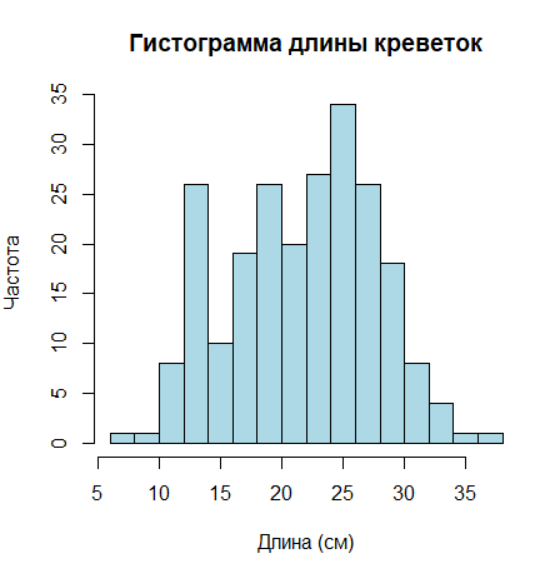
\includegraphics[width=0.6\linewidth,height=\textheight,keepaspectratio]{images/hist_shrimp.PNG}

}

\caption{Рис. 1.1: Гистограмма длины креветок}

\end{figure}%

\subsection{\texorpdfstring{Визуализация в
\texttt{ggridges}}{Визуализация в ggridges}}\label{ux432ux438ux437ux443ux430ux43bux438ux437ux430ux446ux438ux44f-ux432-ggridges}

Для элегантных и компактных графиков подходит библиотека
\texttt{ggridges}. Посторим распределение длины креветки в зависимости
от пола и возраста.

\begin{Shaded}
\begin{Highlighting}[]
\FunctionTok{library}\NormalTok{(ggplot2)}
\FunctionTok{library}\NormalTok{(ggridges)}

\FunctionTok{ggplot}\NormalTok{(data, }\FunctionTok{aes}\NormalTok{(}\AttributeTok{x =}\NormalTok{ length, }
                 \AttributeTok{y =}\NormalTok{ sex, }
                 \AttributeTok{group =}\NormalTok{ sex, }
                 \AttributeTok{fill =}\NormalTok{ sex)) }\SpecialCharTok{+}
  \FunctionTok{geom\_density\_ridges}\NormalTok{(}\AttributeTok{scale =} \DecValTok{2}\NormalTok{, }\AttributeTok{alpha =} \FloatTok{0.7}\NormalTok{) }\SpecialCharTok{+}
  \FunctionTok{scale\_y\_discrete}\NormalTok{(}\AttributeTok{expand =} \FunctionTok{c}\NormalTok{(}\DecValTok{0}\NormalTok{, }\DecValTok{0}\NormalTok{)) }\SpecialCharTok{+}
  \FunctionTok{scale\_x\_continuous}\NormalTok{(}\AttributeTok{expand =} \FunctionTok{c}\NormalTok{(}\DecValTok{0}\NormalTok{, }\DecValTok{0}\NormalTok{)) }\SpecialCharTok{+}
  \FunctionTok{labs}\NormalTok{(}
    \AttributeTok{title =} \StringTok{"Распределение длины карапакса по полу"}\NormalTok{,}
    \AttributeTok{x =} \StringTok{"Длина карапакса (мм)"}\NormalTok{,}
    \AttributeTok{y =} \StringTok{"Пол"}
\NormalTok{  ) }\SpecialCharTok{+}
  \FunctionTok{theme}\NormalTok{(}
    \AttributeTok{panel.border =} \FunctionTok{element\_blank}\NormalTok{(),  }\CommentTok{\# Убирает рамку вокруг графика}
    \AttributeTok{axis.line =} \FunctionTok{element\_line}\NormalTok{(}\AttributeTok{color =} \StringTok{"black"}\NormalTok{)  }\CommentTok{\# Сохраняет осевые линии (опционально)}
\NormalTok{  )}
\end{Highlighting}
\end{Shaded}

\begin{figure}[H]

{\centering 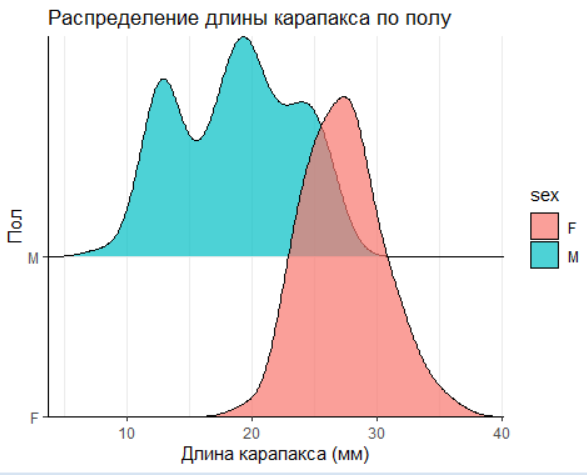
\includegraphics[width=0.6\linewidth,height=\textheight,keepaspectratio]{images/ggridges_shrimp.PNG}

}

\caption{Рис. 1.2: Пол-длина креветок с использованием
\texttt{ggridges}}

\end{figure}%

\section{Выявление аутлайеров
(выбросов)}\label{ux432ux44bux44fux432ux43bux435ux43dux438ux435-ux430ux443ux442ux43bux430ux439ux435ux440ux43eux432-ux432ux44bux431ux440ux43eux441ux43eux432}

Аутлаеры (выбросы) --- наблюдения, значительно отклоняющиеся от общего
распределения данных. Их идентификация критически важна, так как они
могут искажать результаты анализа. Один из надёжных методов обнаружения
выбросов --- \textbf{метод межквартильного размаха (IQR)}.

\subsection{\texorpdfstring{\textbf{Теория
метода}}{Теория метода}}\label{ux442ux435ux43eux440ux438ux44f-ux43cux435ux442ux43eux434ux430}

\begin{enumerate}
\def\labelenumi{\arabic{enumi}.}
\item
  \textbf{Расчёт квартилей}:

  \begin{itemize}
  \item
    \textbf{Q1} (25-й перцентиль): значение, ниже которого находится
    25\% данных.
  \item
    \textbf{Q3} (75-й перцентиль): значение, ниже которого находится
    75\% данных.
  \item
    \textbf{IQR = Q3 - Q1}: мера разброса средней половины данных.
  \end{itemize}
\item
  \textbf{Границы аутлаеров}:

  \begin{itemize}
  \item
    \textbf{Нижняя граница}: Q1−1.5×IQRQ1−1.5×IQR
  \item
    \textbf{Верхняя граница}: Q3+1.5×IQRQ3+1.5×IQR\\
    Наблюдения за этими пределами считаются выбросами.
  \end{itemize}
\end{enumerate}

\subsection{\texorpdfstring{\textbf{Преимущества
метода}}{Преимущества метода}}\label{ux43fux440ux435ux438ux43cux443ux449ux435ux441ux442ux432ux430-ux43cux435ux442ux43eux434ux430}

\begin{itemize}
\item
  Устойчивость к асимметрии распределения.
\item
  Не требует предположения о нормальности данных.
\end{itemize}

\begin{Shaded}
\begin{Highlighting}[]
\CommentTok{\# Метод межквартильного размаха}
\NormalTok{outliers }\OtherTok{\textless{}{-}}\NormalTok{ data }\SpecialCharTok{\%\textgreater{}\%}
  \FunctionTok{mutate}\NormalTok{(}
    \AttributeTok{length\_z =} \FunctionTok{scale}\NormalTok{(length),}
    \AttributeTok{weight\_z =} \FunctionTok{scale}\NormalTok{(weight)}
\NormalTok{  ) }\SpecialCharTok{\%\textgreater{}\%} 
  \FunctionTok{filter}\NormalTok{(}\FunctionTok{abs}\NormalTok{(length\_z) }\SpecialCharTok{\textgreater{}} \DecValTok{3} \SpecialCharTok{|} \FunctionTok{abs}\NormalTok{(weight\_z) }\SpecialCharTok{\textgreater{}} \DecValTok{3}\NormalTok{)}

\CommentTok{\# Визуализация}
\FunctionTok{ggplot}\NormalTok{(data, }\FunctionTok{aes}\NormalTok{(}\AttributeTok{x =}\NormalTok{ length, }\AttributeTok{y =}\NormalTok{ weight)) }\SpecialCharTok{+}
  \FunctionTok{geom\_point}\NormalTok{(}\FunctionTok{aes}\NormalTok{(}\AttributeTok{color =} \StringTok{"Обычные"}\NormalTok{), }\AttributeTok{alpha =} \FloatTok{0.5}\NormalTok{) }\SpecialCharTok{+}
  \FunctionTok{geom\_point}\NormalTok{(}\AttributeTok{data =}\NormalTok{ outliers, }\FunctionTok{aes}\NormalTok{(}\AttributeTok{color =} \StringTok{"Аутлаеры"}\NormalTok{), }\AttributeTok{size =} \DecValTok{3}\NormalTok{) }\SpecialCharTok{+}
  \FunctionTok{scale\_color\_manual}\NormalTok{(}\AttributeTok{values =} \FunctionTok{c}\NormalTok{(}\StringTok{"Обычные"} \OtherTok{=} \StringTok{"grey50"}\NormalTok{, }\StringTok{"Аутлаеры"} \OtherTok{=} \StringTok{"red"}\NormalTok{)) }\SpecialCharTok{+}
  \FunctionTok{labs}\NormalTok{(}\AttributeTok{title =} \StringTok{"Выявление аномальных наблюдений"}\NormalTok{, }\AttributeTok{color =} \StringTok{"Тип"}\NormalTok{)}
\end{Highlighting}
\end{Shaded}

\begin{figure}[H]

{\centering 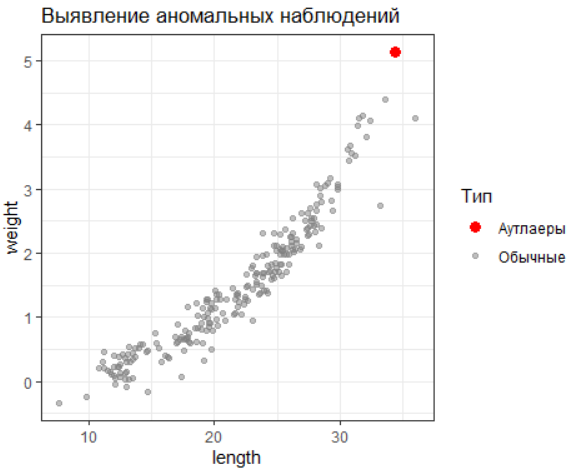
\includegraphics[width=0.6\linewidth,height=\textheight,keepaspectratio]{images/outliers_shrimp.PNG}

}

\caption{Рис. 1.3: Распределение длины карапакса}

\end{figure}%

\section{Определение возрастной структуры: статистические методы анализа
размерных
данных}\label{ux43eux43fux440ux435ux434ux435ux43bux435ux43dux438ux435-ux432ux43eux437ux440ux430ux441ux442ux43dux43eux439-ux441ux442ux440ux443ux43aux442ux443ux440ux44b-ux441ux442ux430ux442ux438ux441ux442ux438ux447ux435ux441ux43aux438ux435-ux43cux435ux442ux43eux434ux44b-ux430ux43dux430ux43bux438ux437ux430-ux440ux430ux437ux43cux435ux440ux43dux44bux445-ux434ux430ux43dux43dux44bux445}

Возрастная структура популяции --- часто важна для расчёта промысловой
смертности, оценки репродуктивного потенциала и прогнозирования динамики
запасов. Поскольку прямое измерение возраста часто невозможно (например,
у беспозвоночных или рыб без четких возрастных меток), используются
статистические методы, выделяющие группы в смешанных распределениях
размеров.

\textbf{Основные подходы:}

\begin{enumerate}
\def\labelenumi{\arabic{enumi}.}
\item
  \textbf{Метод k-средних (k-means)} --- алгоритм кластеризации,
  группирующий особи в заданное число кластеров (возрастных групп) на
  основе их размеров.
\item
  \textbf{Метод Бхаттачарии} --- статистический подход для разделения
  смешанных нормальных распределений, часто применяемый для
  идентификации мод в гистограммах.
\item
  \textbf{EM-алгоритм} --- оценка параметров смеси распределений,
  подходящая для данных с перекрывающимися возрастными группами.
\item
  \textbf{Гауссовы смеси (GMM)} --- расширение метода Бхаттачарии для
  многомерного анализа.
\item
  \textbf{Ядерное сглаживание} --- непараметрический метод визуализации
  плотности, помогающий выявить скрытые моды.
\end{enumerate}

Рассмотрим метод k-средних (k-means) и метод Бхаттачарии, предварительно
построив гистограмму.

\begin{Shaded}
\begin{Highlighting}[]
\CommentTok{\# Загрузка библиотек}
\FunctionTok{library}\NormalTok{(tidyverse)}
\FunctionTok{library}\NormalTok{(mixtools)}
\CommentTok{\# Гистограмма длины с наложением плотности}
\FunctionTok{ggplot}\NormalTok{(data, }\FunctionTok{aes}\NormalTok{(}\AttributeTok{x =}\NormalTok{ length)) }\SpecialCharTok{+}
  \FunctionTok{geom\_histogram}\NormalTok{(}\FunctionTok{aes}\NormalTok{(}\AttributeTok{y =} \FunctionTok{after\_stat}\NormalTok{(density)), }\AttributeTok{fill =} \StringTok{"steelblue"}\NormalTok{, }\AttributeTok{bins =} \DecValTok{20}\NormalTok{, }\AttributeTok{alpha =} \FloatTok{0.7}\NormalTok{) }\SpecialCharTok{+}
  \FunctionTok{geom\_density}\NormalTok{(}\AttributeTok{color =} \StringTok{"\#FC4E07"}\NormalTok{, }\AttributeTok{linewidth =} \DecValTok{1}\NormalTok{) }\SpecialCharTok{+}
  \FunctionTok{labs}\NormalTok{(}\AttributeTok{title =} \StringTok{"Распределение длины карапакса"}\NormalTok{, }
       \AttributeTok{subtitle =} \StringTok{"Пики могут соответствовать возрастным группам"}\NormalTok{,}
       \AttributeTok{x =} \StringTok{"Длина (мм)"}\NormalTok{)}
\end{Highlighting}
\end{Shaded}

\begin{figure}[H]

{\centering 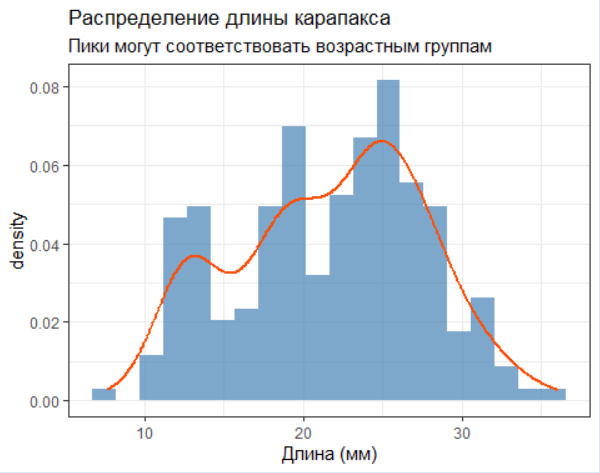
\includegraphics[width=0.6\linewidth,height=\textheight,keepaspectratio]{images/hist_dens_shrimp.PNG}

}

\caption{Рис. 1.3: Распределение длины карапакса}

\end{figure}%

\begin{Shaded}
\begin{Highlighting}[]
\CommentTok{\# Кластеризация по длине (K{-}means как пример)}
\FunctionTok{set.seed}\NormalTok{(}\DecValTok{123}\NormalTok{)}
\NormalTok{clusters }\OtherTok{\textless{}{-}} \FunctionTok{kmeans}\NormalTok{(data}\SpecialCharTok{$}\NormalTok{length, }\AttributeTok{centers =} \DecValTok{4}\NormalTok{)  }\CommentTok{\# Предполагаем 4 возрастные группы}
\NormalTok{data}\SpecialCharTok{$}\NormalTok{cluster }\OtherTok{\textless{}{-}} \FunctionTok{factor}\NormalTok{(clusters}\SpecialCharTok{$}\NormalTok{cluster)}

\CommentTok{\# Визуализация кластеров}
\FunctionTok{ggplot}\NormalTok{(data, }\FunctionTok{aes}\NormalTok{(}\AttributeTok{x =}\NormalTok{ length, }\AttributeTok{fill =}\NormalTok{ cluster)) }\SpecialCharTok{+}
  \FunctionTok{geom\_histogram}\NormalTok{(}\AttributeTok{bins =} \DecValTok{25}\NormalTok{, }\AttributeTok{alpha =} \FloatTok{0.7}\NormalTok{) }\SpecialCharTok{+}
  \FunctionTok{labs}\NormalTok{(}\AttributeTok{title =} \StringTok{"Кластеризация по длине)"}\NormalTok{, }
       \AttributeTok{x =} \StringTok{"Длина (мм)"}\NormalTok{)}
\end{Highlighting}
\end{Shaded}

\begin{figure}[H]

{\centering 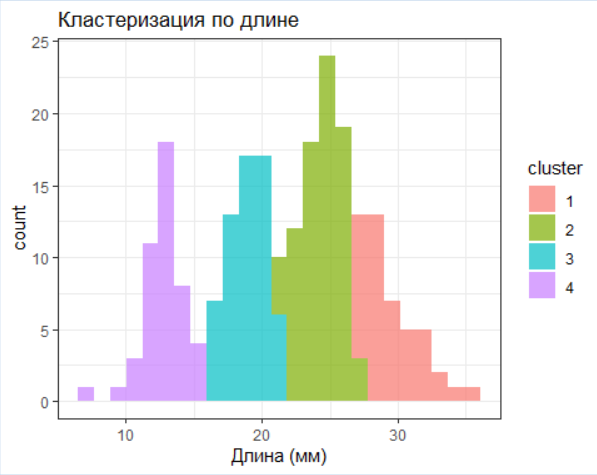
\includegraphics[width=0.6\linewidth,height=\textheight,keepaspectratio]{images/cluster_shrimp.PNG}

}

\caption{Рис. 1.4: Кластеризация по длине}

\end{figure}%

\begin{Shaded}
\begin{Highlighting}[]
\CommentTok{\# Установка рабочей директории}
\FunctionTok{setwd}\NormalTok{(}\StringTok{"C:/TEXTBOOK/"}\NormalTok{)}

\CommentTok{\# Загрузка библиотек}
\FunctionTok{library}\NormalTok{(tidyverse)}
\FunctionTok{library}\NormalTok{(mixtools)}

\CommentTok{\# Загрузка данных}
\NormalTok{data }\OtherTok{\textless{}{-}} \FunctionTok{read.csv}\NormalTok{(}\StringTok{"shrimp\_catch.csv"}\NormalTok{)}

\CommentTok{\# 1. Построение и отображение гистограммы}
\FunctionTok{hist}\NormalTok{(data}\SpecialCharTok{$}\NormalTok{length, }\AttributeTok{breaks =} \DecValTok{20}\NormalTok{, }\AttributeTok{main =} \StringTok{"Гистограмма распределения длин карапаксов"}\NormalTok{,}
     \AttributeTok{xlab =} \StringTok{"Длина карапакса (мм)"}\NormalTok{, }\AttributeTok{ylab =} \StringTok{"Частота"}\NormalTok{)}

\CommentTok{\# 2. Инициализация параметров (предположим 4 возрастные группы)}
\NormalTok{init\_params }\OtherTok{\textless{}{-}} \FunctionTok{list}\NormalTok{(}
  \AttributeTok{lambda =} \FunctionTok{rep}\NormalTok{(}\DecValTok{1}\SpecialCharTok{/}\DecValTok{4}\NormalTok{, }\DecValTok{4}\NormalTok{),}
  \AttributeTok{mu =} \FunctionTok{c}\NormalTok{(}\DecValTok{13}\NormalTok{, }\DecValTok{19}\NormalTok{, }\DecValTok{25}\NormalTok{, }\DecValTok{32}\NormalTok{),}
  \AttributeTok{sigma =} \FunctionTok{c}\NormalTok{(}\FloatTok{1.5}\NormalTok{, }\FloatTok{1.75}\NormalTok{, }\FloatTok{1.75}\NormalTok{, }\FloatTok{2.5}\NormalTok{)}
\NormalTok{)}

\CommentTok{\# 3. Разделение смеси распределений методом EM}
\NormalTok{fit }\OtherTok{\textless{}{-}} \FunctionTok{normalmixEM}\NormalTok{(data}\SpecialCharTok{$}\NormalTok{length, }\AttributeTok{k =} \DecValTok{4}\NormalTok{, }\AttributeTok{maxit =} \DecValTok{1000}\NormalTok{, }\AttributeTok{epsilon =} \FloatTok{1e{-}3}\NormalTok{,}
                   \AttributeTok{lambda =}\NormalTok{ init\_params}\SpecialCharTok{$}\NormalTok{lambda,}
                   \AttributeTok{mu =}\NormalTok{ init\_params}\SpecialCharTok{$}\NormalTok{mu,}
                   \AttributeTok{sigma =}\NormalTok{ init\_params}\SpecialCharTok{$}\NormalTok{sigma)}

\CommentTok{\# 4. Визуализация результатов с ggplot2}
\CommentTok{\# Генерация сетки для построения кривых}
\NormalTok{x\_grid }\OtherTok{\textless{}{-}} \FunctionTok{seq}\NormalTok{(}\FunctionTok{min}\NormalTok{(data}\SpecialCharTok{$}\NormalTok{length), }\FunctionTok{max}\NormalTok{(data}\SpecialCharTok{$}\NormalTok{length), }\AttributeTok{length.out =} \DecValTok{500}\NormalTok{)}

\CommentTok{\# Функция смеси}
\NormalTok{mixture\_density }\OtherTok{\textless{}{-}} \ControlFlowTok{function}\NormalTok{(x) \{}
\NormalTok{  fit}\SpecialCharTok{$}\NormalTok{lambda[}\DecValTok{1}\NormalTok{] }\SpecialCharTok{*} \FunctionTok{dnorm}\NormalTok{(x, fit}\SpecialCharTok{$}\NormalTok{mu[}\DecValTok{1}\NormalTok{], fit}\SpecialCharTok{$}\NormalTok{sigma[}\DecValTok{1}\NormalTok{]) }\SpecialCharTok{+}
\NormalTok{  fit}\SpecialCharTok{$}\NormalTok{lambda[}\DecValTok{2}\NormalTok{] }\SpecialCharTok{*} \FunctionTok{dnorm}\NormalTok{(x, fit}\SpecialCharTok{$}\NormalTok{mu[}\DecValTok{2}\NormalTok{], fit}\SpecialCharTok{$}\NormalTok{sigma[}\DecValTok{2}\NormalTok{]) }\SpecialCharTok{+}
\NormalTok{  fit}\SpecialCharTok{$}\NormalTok{lambda[}\DecValTok{3}\NormalTok{] }\SpecialCharTok{*} \FunctionTok{dnorm}\NormalTok{(x, fit}\SpecialCharTok{$}\NormalTok{mu[}\DecValTok{3}\NormalTok{], fit}\SpecialCharTok{$}\NormalTok{sigma[}\DecValTok{3}\NormalTok{]) }\SpecialCharTok{+}
\NormalTok{  fit}\SpecialCharTok{$}\NormalTok{lambda[}\DecValTok{4}\NormalTok{] }\SpecialCharTok{*} \FunctionTok{dnorm}\NormalTok{(x, fit}\SpecialCharTok{$}\NormalTok{mu[}\DecValTok{4}\NormalTok{], fit}\SpecialCharTok{$}\NormalTok{sigma[}\DecValTok{4}\NormalTok{])}
\NormalTok{\}}

\CommentTok{\# График}
\FunctionTok{ggplot}\NormalTok{(data, }\FunctionTok{aes}\NormalTok{(}\AttributeTok{x =}\NormalTok{ length)) }\SpecialCharTok{+}
  \CommentTok{\# Гистограмма}
  \FunctionTok{geom\_histogram}\NormalTok{(}\FunctionTok{aes}\NormalTok{(}\AttributeTok{y =} \FunctionTok{after\_stat}\NormalTok{(density)), }\AttributeTok{bins =} \DecValTok{20}\NormalTok{, }\AttributeTok{fill =} \StringTok{"white"}\NormalTok{, }\AttributeTok{color =} \StringTok{"black"}\NormalTok{, }\AttributeTok{alpha =} \FloatTok{0.7}\NormalTok{) }\SpecialCharTok{+}
  \CommentTok{\# Исходное распределение (гладкая линия)}
  \FunctionTok{geom\_density}\NormalTok{(}\AttributeTok{color =} \StringTok{"red"}\NormalTok{, }\AttributeTok{lwd =} \FloatTok{1.2}\NormalTok{) }\SpecialCharTok{+}
  \CommentTok{\# Смесь распределений}
  \FunctionTok{stat\_function}\NormalTok{(}\AttributeTok{fun =}\NormalTok{ mixture\_density, }\AttributeTok{color =} \StringTok{"black"}\NormalTok{, }\AttributeTok{lwd =} \FloatTok{1.5}\NormalTok{) }\SpecialCharTok{+}
  \CommentTok{\# Компоненты смеси}
  \FunctionTok{stat\_function}\NormalTok{(}\AttributeTok{fun =} \ControlFlowTok{function}\NormalTok{(x) fit}\SpecialCharTok{$}\NormalTok{lambda[}\DecValTok{1}\NormalTok{] }\SpecialCharTok{*} \FunctionTok{dnorm}\NormalTok{(x, fit}\SpecialCharTok{$}\NormalTok{mu[}\DecValTok{1}\NormalTok{], fit}\SpecialCharTok{$}\NormalTok{sigma[}\DecValTok{1}\NormalTok{]), }\AttributeTok{color =} \StringTok{"blue"}\NormalTok{, }\AttributeTok{lwd =} \DecValTok{1}\NormalTok{) }\SpecialCharTok{+}
  \FunctionTok{stat\_function}\NormalTok{(}\AttributeTok{fun =} \ControlFlowTok{function}\NormalTok{(x) fit}\SpecialCharTok{$}\NormalTok{lambda[}\DecValTok{2}\NormalTok{] }\SpecialCharTok{*} \FunctionTok{dnorm}\NormalTok{(x, fit}\SpecialCharTok{$}\NormalTok{mu[}\DecValTok{2}\NormalTok{], fit}\SpecialCharTok{$}\NormalTok{sigma[}\DecValTok{2}\NormalTok{]), }\AttributeTok{color =} \StringTok{"green"}\NormalTok{, }\AttributeTok{lwd =} \DecValTok{1}\NormalTok{) }\SpecialCharTok{+}
  \FunctionTok{stat\_function}\NormalTok{(}\AttributeTok{fun =} \ControlFlowTok{function}\NormalTok{(x) fit}\SpecialCharTok{$}\NormalTok{lambda[}\DecValTok{3}\NormalTok{] }\SpecialCharTok{*} \FunctionTok{dnorm}\NormalTok{(x, fit}\SpecialCharTok{$}\NormalTok{mu[}\DecValTok{3}\NormalTok{], fit}\SpecialCharTok{$}\NormalTok{sigma[}\DecValTok{3}\NormalTok{]), }\AttributeTok{color =} \StringTok{"orange"}\NormalTok{, }\AttributeTok{lwd =} \DecValTok{1}\NormalTok{) }\SpecialCharTok{+}
  \FunctionTok{stat\_function}\NormalTok{(}\AttributeTok{fun =} \ControlFlowTok{function}\NormalTok{(x) fit}\SpecialCharTok{$}\NormalTok{lambda[}\DecValTok{4}\NormalTok{] }\SpecialCharTok{*} \FunctionTok{dnorm}\NormalTok{(x, fit}\SpecialCharTok{$}\NormalTok{mu[}\DecValTok{4}\NormalTok{], fit}\SpecialCharTok{$}\NormalTok{sigma[}\DecValTok{4}\NormalTok{]), }\AttributeTok{color =} \StringTok{"purple"}\NormalTok{, }\AttributeTok{lwd =} \DecValTok{1}\NormalTok{) }\SpecialCharTok{+}
  
  \CommentTok{\# Настройка темы и легенды}
  \FunctionTok{theme\_minimal}\NormalTok{() }\SpecialCharTok{+}
  \FunctionTok{labs}\NormalTok{(}
    \AttributeTok{x =} \StringTok{"Длина карапакса (мм)"}\NormalTok{,}
    \AttributeTok{y =} \StringTok{"Плотность"}\NormalTok{,}
    \AttributeTok{title =} \StringTok{"Разделение возрастных групп методом EM"}
\NormalTok{  )}
\end{Highlighting}
\end{Shaded}

\begin{figure}[H]

{\centering 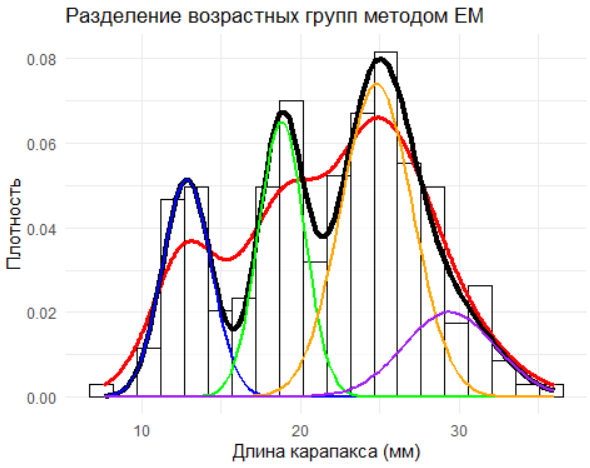
\includegraphics[width=0.6\linewidth,height=\textheight,keepaspectratio]{images/bhattacharya_shrimp.PNG}

}

\caption{Рис. 1.5: Метод Бхаттачарии}

\end{figure}%

\section{Уравнение
Берталанфи}\label{ux443ux440ux430ux432ux43dux435ux43dux438ux435-ux431ux435ux440ux442ux430ux43bux430ux43dux444ux438}

Уравнение Берталанфи --- фундаментальная модель в рыбохозяйственной
науке, описывающая асимптотический рост организмов. Оно имеет вид: \[
L(t) = L_{\infty} \cdot \left(1 - e^{-k \cdot (t - t_0)}\right)
\] где \emph{L\textsubscript{∞}}--- теоретическая максимальная длина
особи, \emph{k}--- коэффициент скорости роста,
\emph{t\textsubscript{0}}--- гипотетический возраст при нулевой длине.

В приведённом коде модель применяется для анализа роста северной
креветки :

\begin{enumerate}
\def\labelenumi{\arabic{enumi}.}
\item
  \textbf{Подготовка данных}: Удаление аутлаеров (например, строк 10 и
  50) повышает точность оценки параметров.
\item
  \textbf{Инициализация параметров}:

  \begin{itemize}
  \item
    \emph{L\textsubscript{∞}} задаётся как максимальная наблюдаемая
    длина в данных.
  \item
    \emph{k} и \emph{t\textsubscript{0}} подбираются итеративно методом
    нелинейных наименьших квадратов (\textbf{\texttt{nls}}).
  \end{itemize}
\item
  \textbf{Визуализация}: График сопоставляет эмпирические данные (точки)
  с предсказаниями модели (красная линия), демонстрируя, как рост
  замедляется с приближением к \emph{L∞}.
\end{enumerate}

\textbf{Интерпретация параметров}:

\begin{itemize}
\item
  Высокое значение \emph{k} (\textgreater0.3) указывает на быстрый рост
  молоди.
\item
  \emph{t\textsubscript{0}}\textless0 может отражать ранний метаморфоз
  личинок.
\end{itemize}

\begin{Shaded}
\begin{Highlighting}[]
\CommentTok{\# Загрузка библиотек}
\FunctionTok{library}\NormalTok{(ggplot2)}
\FunctionTok{library}\NormalTok{(dplyr)}
\FunctionTok{library}\NormalTok{(nlme)}

\CommentTok{\# Загрузка данных}
\NormalTok{data }\OtherTok{\textless{}{-}} \FunctionTok{read.csv}\NormalTok{(}\StringTok{"shrimp\_catch.csv"}\NormalTok{)}

\CommentTok{\# Преобразование возраста в числовой формат}
\NormalTok{data}\SpecialCharTok{$}\NormalTok{age\_num }\OtherTok{\textless{}{-}} \FunctionTok{as.numeric}\NormalTok{(data}\SpecialCharTok{$}\NormalTok{age)}

\CommentTok{\# Удаление аутлайеров (если необходимо)}
\NormalTok{data\_clean }\OtherTok{\textless{}{-}}\NormalTok{ data }\SpecialCharTok{\%\textgreater{}\%}
  \FunctionTok{filter}\NormalTok{(}\SpecialCharTok{!}\NormalTok{id }\SpecialCharTok{\%in\%} \FunctionTok{c}\NormalTok{(}\DecValTok{10}\NormalTok{, }\DecValTok{50}\NormalTok{))  }\CommentTok{\# Пример удаления строк с аномалиями}

\CommentTok{\# Начальные параметры на основе данных}
\NormalTok{L\_inf\_start }\OtherTok{\textless{}{-}} \FunctionTok{max}\NormalTok{(data\_clean}\SpecialCharTok{$}\NormalTok{length, }\AttributeTok{na.rm =} \ConstantTok{TRUE}\NormalTok{)  }\CommentTok{\# Максимальная длина}
\NormalTok{k\_start }\OtherTok{\textless{}{-}} \FloatTok{0.3}                                        \CommentTok{\# Средняя скорость роста}
\NormalTok{t0\_start }\OtherTok{\textless{}{-}} \SpecialCharTok{{-}}\FloatTok{0.5}                                      \CommentTok{\# Гипотетический возраст}

\CommentTok{\# Подгонка модели с увеличенным числом итераций}
\NormalTok{model }\OtherTok{\textless{}{-}} \FunctionTok{nls}\NormalTok{(}
\NormalTok{  length }\SpecialCharTok{\textasciitilde{}}\NormalTok{ L\_inf }\SpecialCharTok{*}\NormalTok{ (}\DecValTok{1} \SpecialCharTok{{-}} \FunctionTok{exp}\NormalTok{(}\SpecialCharTok{{-}}\NormalTok{k }\SpecialCharTok{*}\NormalTok{ (age\_num }\SpecialCharTok{{-}}\NormalTok{ t0))),}
  \AttributeTok{data =}\NormalTok{ data\_clean,}
  \AttributeTok{start =} \FunctionTok{list}\NormalTok{(}\AttributeTok{L\_inf =}\NormalTok{ L\_inf\_start, }\AttributeTok{k =}\NormalTok{ k\_start, }\AttributeTok{t0 =}\NormalTok{ t0\_start),}
  \AttributeTok{control =} \FunctionTok{nls.control}\NormalTok{(}\AttributeTok{maxiter =} \DecValTok{200}\NormalTok{, }\AttributeTok{warnOnly =} \ConstantTok{TRUE}\NormalTok{)  }\CommentTok{\# Увеличиваем лимит итераций}
\NormalTok{)}

\CommentTok{\# Вывод результатов}
\FunctionTok{summary}\NormalTok{(model)}

\CommentTok{\# Создание последовательности возрастов для предсказания}
\NormalTok{age\_seq }\OtherTok{\textless{}{-}} \FunctionTok{seq}\NormalTok{(}\FunctionTok{min}\NormalTok{(data\_clean}\SpecialCharTok{$}\NormalTok{age\_num), }\FunctionTok{max}\NormalTok{(data\_clean}\SpecialCharTok{$}\NormalTok{age\_num), }\AttributeTok{by =} \FloatTok{0.1}\NormalTok{)}

\CommentTok{\# Предсказание значений длины}
\NormalTok{length\_pred }\OtherTok{\textless{}{-}} \FunctionTok{predict}\NormalTok{(model, }\AttributeTok{newdata =} \FunctionTok{data.frame}\NormalTok{(}\AttributeTok{age\_num =}\NormalTok{ age\_seq))}

\CommentTok{\# Построение графика}
\FunctionTok{ggplot}\NormalTok{(data\_clean, }\FunctionTok{aes}\NormalTok{(}\AttributeTok{x =}\NormalTok{ age\_num, }\AttributeTok{y =}\NormalTok{ length)) }\SpecialCharTok{+}
  \FunctionTok{geom\_point}\NormalTok{(}\FunctionTok{aes}\NormalTok{(}\AttributeTok{color =}\NormalTok{ age), }\AttributeTok{alpha =} \FloatTok{0.7}\NormalTok{) }\SpecialCharTok{+}
  \FunctionTok{geom\_line}\NormalTok{(}\AttributeTok{data =} \FunctionTok{data.frame}\NormalTok{(}\AttributeTok{age\_num =}\NormalTok{ age\_seq, }\AttributeTok{length =}\NormalTok{ length\_pred), }
            \FunctionTok{aes}\NormalTok{(}\AttributeTok{x =}\NormalTok{ age\_num, }\AttributeTok{y =}\NormalTok{ length), }\AttributeTok{color =} \StringTok{"red"}\NormalTok{, }\AttributeTok{linewidth =} \FloatTok{1.2}\NormalTok{) }\SpecialCharTok{+}
  \FunctionTok{labs}\NormalTok{(}
    \AttributeTok{title =} \StringTok{"Рост креветок по уравнению Берталанфи"}\NormalTok{,}
    \AttributeTok{x =} \StringTok{"Возраст (годы)"}\NormalTok{,}
    \AttributeTok{y =} \StringTok{"Длина карапакса (мм)"}\NormalTok{,}
    \AttributeTok{color =} \StringTok{"Возрастная группа"}
\NormalTok{  ) }\SpecialCharTok{+}
  \FunctionTok{theme\_minimal}\NormalTok{()}

\CommentTok{\# Сохранение графика}
\FunctionTok{ggsave}\NormalTok{(}\StringTok{"bertalanffy\_model.png"}\NormalTok{, }\AttributeTok{width =} \DecValTok{8}\NormalTok{, }\AttributeTok{height =} \DecValTok{6}\NormalTok{)}
\end{Highlighting}
\end{Shaded}

\begin{figure}[H]

{\centering 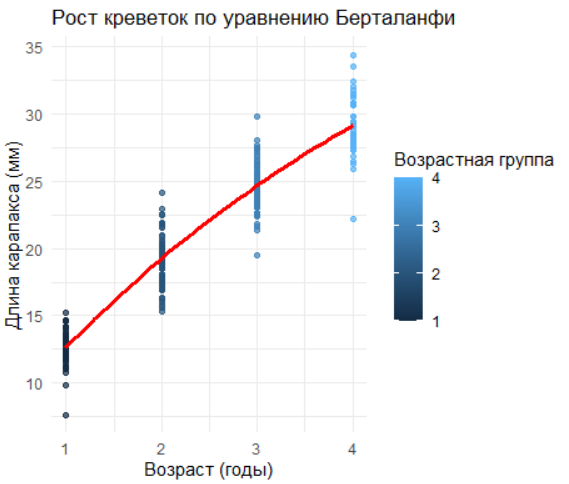
\includegraphics[width=0.6\linewidth,height=\textheight,keepaspectratio]{images/bertalanffy_model.PNG}

}

\caption{Рис. 1.6: Рост креветок по уравнению Берталанфи}

\end{figure}%

\section{Огива, логистическая кривая и 50\%-ное
созревание}\label{ux43eux433ux438ux432ux430-ux43bux43eux433ux438ux441ux442ux438ux447ux435ux441ux43aux430ux44f-ux43aux440ux438ux432ux430ux44f-ux438-50-ux43dux43eux435-ux441ux43eux437ux440ux435ux432ux430ux43dux438ux435}

Логистическая кривая --- ключевой инструмент для моделирования бинарных
процессов, таких как созревание или смена пола у организмов. В случае
протоандрических креветок (\emph{Pandalus borealis}), которые меняют пол
с возрастом, зависимость вероятности быть самкой от длины карапакса
можно описать логистической функцией:

\[
P(F) = \frac{1}{1 + e^{-(\beta_0 + \beta_1 \cdot длина)}}
\]

где \emph{P(F)} --- вероятность принадлежности к женскому полу,
\emph{β\textsubscript{0}} --- интерсепт, \emph{β\textsubscript{1}} ---
коэффициент влияния длины.

Точка перегиба логистической кривой соответствует длине, при которой
вероятность быть самкой равна 50\%: \[
L_{50} = -\frac{\beta_0}{\beta_1}
\]

\begin{figure}[H]

{\centering 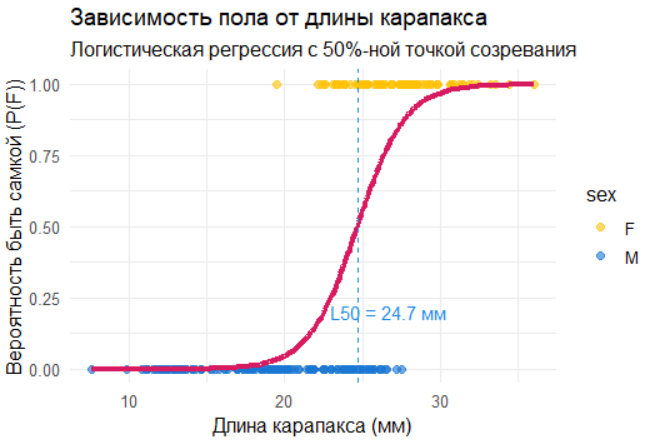
\includegraphics[width=0.6\linewidth,height=\textheight,keepaspectratio]{images/logistic_model_shrimp.PNG}

}

\caption{Рис. 1.7: Логистическая кривая}

\end{figure}%

Огива (кумулятивная кривая) показывает накопление вероятности с
увеличением длины. Для анализа созревания её можно построить через
интеграл логистической функции. Визуально она демонстрирует, как доля
самок возрастает с размером.

\begin{figure}[H]

{\centering 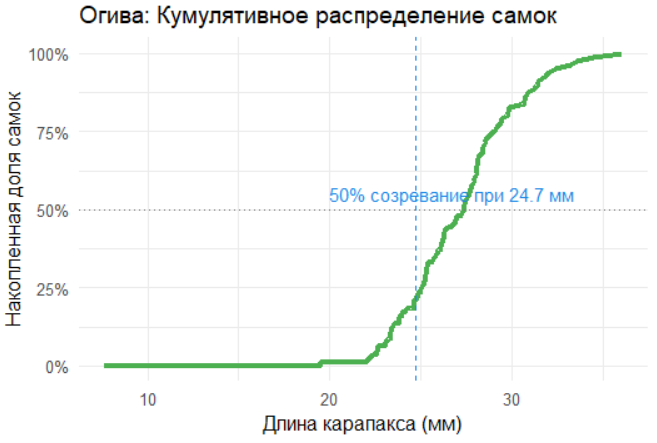
\includegraphics[width=0.6\linewidth,height=\textheight,keepaspectratio]{images/ogive_shrimp.PNG}

}

\caption{Рис. 1.8: Огива}

\end{figure}%

\subsection{\texorpdfstring{\textbf{Оценка
модели}}{Оценка модели}}\label{ux43eux446ux435ux43dux43aux430-ux43cux43eux434ux435ux43bux438}

\begin{enumerate}
\def\labelenumi{\arabic{enumi}.}
\item
  \textbf{ROC-кривая и AUC}:

  \begin{itemize}
  \item
    Площадь под ROC-кривой (AUC) \textgreater0.7 указывает на хорошую
    предсказательную способность модели.
  \item
    Значение AUC = 0.94(пример из кода) подтверждает сильную связь длины
    и пола.
  \end{itemize}
\end{enumerate}

\begin{figure}[H]

{\centering 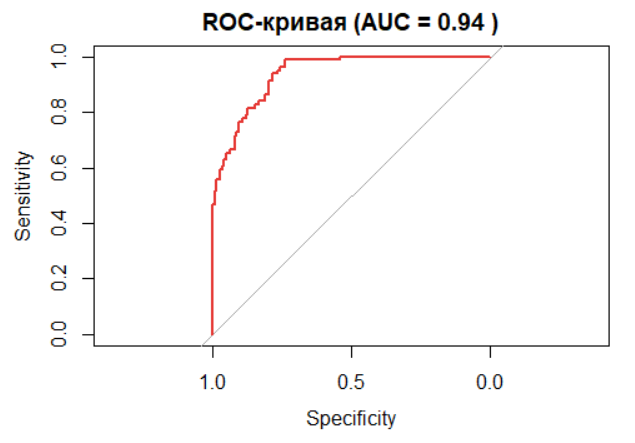
\includegraphics[width=0.6\linewidth,height=\textheight,keepaspectratio]{images/ROC_shrimp.PNG}

}

\caption{Рис. 1.9: ROC-кривая и AUC}

\end{figure}%

\begin{enumerate}
\def\labelenumi{\arabic{enumi}.}
\setcounter{enumi}{1}
\item
  \textbf{Интерпретация коэффициентов}:

  \begin{itemize}
  \item
    Положительный \emph{β\textsubscript{1}} означает: с ростом длины
    вероятность быть самкой увеличивается.
  \item
    Например, \emph{β\textsubscript{1}}=0.25 → увеличение длины на 1 мм
    повышает шансы в e\textsuperscript{0.25}≈1.28 раза.
  \end{itemize}
\end{enumerate}

\subsection{\texorpdfstring{\textbf{Биологический
контекст}}{Биологический контекст}}\label{ux431ux438ux43eux43bux43eux433ux438ux447ux435ux441ux43aux438ux439-ux43aux43eux43dux442ux435ux43aux441ux442}

\begin{itemize}
\item
  \textbf{Протоандрический гермафродитизм}: У креветок смена пола с
  самцов на самок происходит при достижении критического размера
  (\textasciitilde25-28 мм).
\item
  \textbf{L50 как индикатор}: Снижение \emph{L\textsubscript{50}} в
  популяции может сигнализировать о стрессовых условиях (перелов,
  изменение среды), ускоряющих созревание.
\end{itemize}

\begin{Shaded}
\begin{Highlighting}[]
\CommentTok{\# Установка рабочей директории}
\FunctionTok{setwd}\NormalTok{(}\StringTok{"C:/TEXTBOOK/"}\NormalTok{)}

\CommentTok{\# Загрузка библиотек}
\FunctionTok{library}\NormalTok{(tidyverse)}
\FunctionTok{library}\NormalTok{(pROC)}
\FunctionTok{library}\NormalTok{(ggplot2)}

\CommentTok{\# Загрузка данных}
\NormalTok{data }\OtherTok{\textless{}{-}} \FunctionTok{read\_csv}\NormalTok{(}\StringTok{"shrimp\_catch.csv"}\NormalTok{)}

\CommentTok{\# 1. Предобработка данных {-}{-}{-}{-}{-}{-}{-}{-}{-}{-}{-}{-}{-}{-}{-}{-}{-}{-}{-}{-}{-}{-}{-}{-}{-}{-}{-}{-}{-}{-}{-}{-}{-}{-}{-}{-}{-}{-}{-}{-}{-}{-}{-}{-}{-}{-}{-}{-}{-}{-}{-}{-}{-}}
\CommentTok{\# Удаление аутлаеров методом IQR}
\NormalTok{Q1 }\OtherTok{\textless{}{-}} \FunctionTok{quantile}\NormalTok{(data}\SpecialCharTok{$}\NormalTok{length, }\FloatTok{0.25}\NormalTok{)}
\NormalTok{Q3 }\OtherTok{\textless{}{-}} \FunctionTok{quantile}\NormalTok{(data}\SpecialCharTok{$}\NormalTok{length, }\FloatTok{0.75}\NormalTok{)}
\NormalTok{IQR }\OtherTok{\textless{}{-}}\NormalTok{ Q3 }\SpecialCharTok{{-}}\NormalTok{ Q1}
\NormalTok{data\_clean }\OtherTok{\textless{}{-}}\NormalTok{ data }\SpecialCharTok{\%\textgreater{}\%}
  \FunctionTok{filter}\NormalTok{(length }\SpecialCharTok{\textgreater{}=}\NormalTok{ Q1 }\SpecialCharTok{{-}} \FloatTok{1.5}\SpecialCharTok{*}\NormalTok{IQR }\SpecialCharTok{\&}\NormalTok{ length }\SpecialCharTok{\textless{}=}\NormalTok{ Q3 }\SpecialCharTok{+} \FloatTok{1.5}\SpecialCharTok{*}\NormalTok{IQR)}

\CommentTok{\# 2. Логистическая регрессия {-}{-}{-}{-}{-}{-}{-}{-}{-}{-}{-}{-}{-}{-}{-}{-}{-}{-}{-}{-}{-}{-}{-}{-}{-}{-}{-}{-}{-}{-}{-}{-}{-}{-}{-}{-}{-}{-}{-}{-}{-}{-}{-}{-}{-}{-}{-}{-}{-}{-}}
\CommentTok{\# Преобразование пола в бинарную переменную}
\NormalTok{data\_clean}\SpecialCharTok{$}\NormalTok{sex\_binary }\OtherTok{\textless{}{-}} \FunctionTok{ifelse}\NormalTok{(data\_clean}\SpecialCharTok{$}\NormalTok{sex }\SpecialCharTok{==} \StringTok{"F"}\NormalTok{, }\DecValTok{1}\NormalTok{, }\DecValTok{0}\NormalTok{)}

\CommentTok{\# Подгонка модели}
\NormalTok{model\_logit }\OtherTok{\textless{}{-}} \FunctionTok{glm}\NormalTok{(sex\_binary }\SpecialCharTok{\textasciitilde{}}\NormalTok{ length, }
                   \AttributeTok{data =}\NormalTok{ data\_clean, }
                   \AttributeTok{family =} \FunctionTok{binomial}\NormalTok{(}\AttributeTok{link =} \StringTok{"logit"}\NormalTok{))}

\CommentTok{\# Расчет коэффициентов}
\NormalTok{beta0 }\OtherTok{\textless{}{-}} \FunctionTok{coef}\NormalTok{(model\_logit)[}\DecValTok{1}\NormalTok{]}
\NormalTok{beta1 }\OtherTok{\textless{}{-}} \FunctionTok{coef}\NormalTok{(model\_logit)[}\DecValTok{2}\NormalTok{]}

\CommentTok{\# Вычисление L50 (длина 50\% созревания)}
\NormalTok{L50 }\OtherTok{\textless{}{-}} \FunctionTok{round}\NormalTok{(}\SpecialCharTok{{-}}\NormalTok{beta0}\SpecialCharTok{/}\NormalTok{beta1, }\DecValTok{1}\NormalTok{)}

\CommentTok{\# 3. Визуализация {-}{-}{-}{-}{-}{-}{-}{-}{-}{-}{-}{-}{-}{-}{-}{-}{-}{-}{-}{-}{-}{-}{-}{-}{-}{-}{-}{-}{-}{-}{-}{-}{-}{-}{-}{-}{-}{-}{-}{-}{-}{-}{-}{-}{-}{-}{-}{-}{-}{-}{-}{-}{-}{-}{-}{-}{-}{-}{-}{-}}
\CommentTok{\# Логистическая кривая}
\FunctionTok{ggplot}\NormalTok{(data\_clean, }\FunctionTok{aes}\NormalTok{(}\AttributeTok{x =}\NormalTok{ length, }\AttributeTok{y =}\NormalTok{ sex\_binary)) }\SpecialCharTok{+}
  \FunctionTok{geom\_point}\NormalTok{(}\FunctionTok{aes}\NormalTok{(}\AttributeTok{color =}\NormalTok{ sex), }\AttributeTok{alpha =} \FloatTok{0.6}\NormalTok{, }\AttributeTok{size =} \DecValTok{2}\NormalTok{) }\SpecialCharTok{+}
  \FunctionTok{geom\_line}\NormalTok{(}\FunctionTok{aes}\NormalTok{(}\AttributeTok{y =} \FunctionTok{predict}\NormalTok{(model\_logit, }\AttributeTok{type =} \StringTok{"response"}\NormalTok{)), }
            \AttributeTok{color =} \StringTok{"\#D81B60"}\NormalTok{, }\AttributeTok{linewidth =} \FloatTok{1.5}\NormalTok{) }\SpecialCharTok{+}
  \FunctionTok{geom\_vline}\NormalTok{(}\AttributeTok{xintercept =}\NormalTok{ L50, }\AttributeTok{linetype =} \StringTok{"dashed"}\NormalTok{, }\AttributeTok{color =} \StringTok{"\#1E88E5"}\NormalTok{) }\SpecialCharTok{+}
  \FunctionTok{annotate}\NormalTok{(}\StringTok{"text"}\NormalTok{, }\AttributeTok{x =}\NormalTok{ L50 }\SpecialCharTok{+} \DecValTok{2}\NormalTok{, }\AttributeTok{y =} \FloatTok{0.2}\NormalTok{, }
           \AttributeTok{label =} \FunctionTok{paste}\NormalTok{(}\StringTok{"L50 ="}\NormalTok{, L50, }\StringTok{"мм"}\NormalTok{), }\AttributeTok{color =} \StringTok{"\#1E88E5"}\NormalTok{) }\SpecialCharTok{+}
  \FunctionTok{scale\_color\_manual}\NormalTok{(}\AttributeTok{values =} \FunctionTok{c}\NormalTok{(}\StringTok{"\#FFC107"}\NormalTok{, }\StringTok{"\#1976D2"}\NormalTok{)) }\SpecialCharTok{+}
  \FunctionTok{labs}\NormalTok{(}
    \AttributeTok{title =} \StringTok{"Зависимость пола от длины карапакса"}\NormalTok{,}
    \AttributeTok{subtitle =} \StringTok{"Логистическая регрессия с 50\%{-}ной точкой созревания"}\NormalTok{,}
    \AttributeTok{x =} \StringTok{"Длина карапакса (мм)"}\NormalTok{,}
    \AttributeTok{y =} \StringTok{"Вероятность быть самкой (P(F))"}
\NormalTok{  ) }\SpecialCharTok{+}
  \FunctionTok{theme\_minimal}\NormalTok{(}\AttributeTok{base\_size =} \DecValTok{12}\NormalTok{)}

\CommentTok{\# Огива (кумулятивное распределение)}
\NormalTok{data\_ogive }\OtherTok{\textless{}{-}}\NormalTok{ data\_clean }\SpecialCharTok{\%\textgreater{}\%}
  \FunctionTok{arrange}\NormalTok{(length) }\SpecialCharTok{\%\textgreater{}\%}
  \FunctionTok{mutate}\NormalTok{(}
    \AttributeTok{cum\_females =} \FunctionTok{cumsum}\NormalTok{(sex\_binary),}
    \AttributeTok{cum\_prob =}\NormalTok{ cum\_females }\SpecialCharTok{/} \FunctionTok{max}\NormalTok{(cum\_females)}
\NormalTok{  )}

\FunctionTok{ggplot}\NormalTok{(data\_ogive, }\FunctionTok{aes}\NormalTok{(}\AttributeTok{x =}\NormalTok{ length, }\AttributeTok{y =}\NormalTok{ cum\_prob)) }\SpecialCharTok{+}
  \FunctionTok{geom\_line}\NormalTok{(}\AttributeTok{color =} \StringTok{"\#4CAF50"}\NormalTok{, }\AttributeTok{linewidth =} \FloatTok{1.5}\NormalTok{) }\SpecialCharTok{+}
  \FunctionTok{geom\_vline}\NormalTok{(}\AttributeTok{xintercept =}\NormalTok{ L50, }\AttributeTok{linetype =} \StringTok{"dashed"}\NormalTok{, }\AttributeTok{color =} \StringTok{"\#1E88E5"}\NormalTok{) }\SpecialCharTok{+}
  \FunctionTok{geom\_hline}\NormalTok{(}\AttributeTok{yintercept =} \FloatTok{0.5}\NormalTok{, }\AttributeTok{linetype =} \StringTok{"dotted"}\NormalTok{, }\AttributeTok{color =} \StringTok{"\#757575"}\NormalTok{) }\SpecialCharTok{+}
  \FunctionTok{annotate}\NormalTok{(}\StringTok{"text"}\NormalTok{, }\AttributeTok{x =}\NormalTok{ L50 }\SpecialCharTok{+} \DecValTok{2}\NormalTok{, }\AttributeTok{y =} \FloatTok{0.55}\NormalTok{, }
           \AttributeTok{label =} \FunctionTok{paste}\NormalTok{(}\StringTok{"50\% созревание при"}\NormalTok{, L50, }\StringTok{"мм"}\NormalTok{), }\AttributeTok{color =} \StringTok{"\#1E88E5"}\NormalTok{) }\SpecialCharTok{+}
  \FunctionTok{scale\_y\_continuous}\NormalTok{(}\AttributeTok{labels =}\NormalTok{ scales}\SpecialCharTok{::}\NormalTok{percent) }\SpecialCharTok{+}
  \FunctionTok{labs}\NormalTok{(}
    \AttributeTok{title =} \StringTok{"Огива: Кумулятивное распределение самок"}\NormalTok{,}
    \AttributeTok{x =} \StringTok{"Длина карапакса (мм)"}\NormalTok{,}
    \AttributeTok{y =} \StringTok{"Накопленная доля самок"}
\NormalTok{  ) }\SpecialCharTok{+}
  \FunctionTok{theme\_minimal}\NormalTok{(}\AttributeTok{base\_size =} \DecValTok{12}\NormalTok{)}

\CommentTok{\# 4. Оценка модели {-}{-}{-}{-}{-}{-}{-}{-}{-}{-}{-}{-}{-}{-}{-}{-}{-}{-}{-}{-}{-}{-}{-}{-}{-}{-}{-}{-}{-}{-}{-}{-}{-}{-}{-}{-}{-}{-}{-}{-}{-}{-}{-}{-}{-}{-}{-}{-}{-}{-}{-}{-}{-}{-}{-}{-}{-}{-}{-}}
\CommentTok{\# ROC{-}анализ}
\NormalTok{roc\_obj }\OtherTok{\textless{}{-}} \FunctionTok{roc}\NormalTok{(data\_clean}\SpecialCharTok{$}\NormalTok{sex\_binary, }\FunctionTok{predict}\NormalTok{(model\_logit, }\AttributeTok{type =} \StringTok{"response"}\NormalTok{))}
\NormalTok{auc\_value }\OtherTok{\textless{}{-}} \FunctionTok{round}\NormalTok{(}\FunctionTok{auc}\NormalTok{(roc\_obj), }\DecValTok{2}\NormalTok{)}

\CommentTok{\# График ROC{-}кривой}
\FunctionTok{plot}\NormalTok{(roc\_obj, }\AttributeTok{col =} \StringTok{"\#E53935"}\NormalTok{, }\AttributeTok{main =} \FunctionTok{paste}\NormalTok{(}\StringTok{"ROC{-}кривая (AUC ="}\NormalTok{, auc\_value, }\StringTok{")"}\NormalTok{))}

\CommentTok{\# 5. Сохранение результатов {-}{-}{-}{-}{-}{-}{-}{-}{-}{-}{-}{-}{-}{-}{-}{-}{-}{-}{-}{-}{-}{-}{-}{-}{-}{-}{-}{-}{-}{-}{-}{-}{-}{-}{-}{-}{-}{-}{-}{-}{-}{-}{-}{-}{-}{-}{-}{-}{-}{-}}
\FunctionTok{ggsave}\NormalTok{(}\StringTok{"logistic\_curve.png"}\NormalTok{, }\AttributeTok{width =} \DecValTok{8}\NormalTok{, }\AttributeTok{height =} \DecValTok{6}\NormalTok{, }\AttributeTok{dpi =} \DecValTok{300}\NormalTok{)}
\FunctionTok{ggsave}\NormalTok{(}\StringTok{"ogive\_curve.png"}\NormalTok{, }\AttributeTok{width =} \DecValTok{8}\NormalTok{, }\AttributeTok{height =} \DecValTok{6}\NormalTok{, }\AttributeTok{dpi =} \DecValTok{300}\NormalTok{)}

\CommentTok{\# Вывод ключевых метрик}
\FunctionTok{cat}\NormalTok{(}\StringTok{"Результаты анализа:}\SpecialCharTok{\textbackslash{}n}\StringTok{"}\NormalTok{)}
\FunctionTok{cat}\NormalTok{(}\StringTok{"{-} Длина 50\%{-}ного созревания (L50):"}\NormalTok{, L50, }\StringTok{"мм}\SpecialCharTok{\textbackslash{}n}\StringTok{"}\NormalTok{)}
\FunctionTok{cat}\NormalTok{(}\StringTok{"{-} AUC модели:"}\NormalTok{, auc\_value, }\StringTok{"}\SpecialCharTok{\textbackslash{}n}\StringTok{"}\NormalTok{)}
\FunctionTok{cat}\NormalTok{(}\StringTok{"{-} Коэффициенты модели:}\SpecialCharTok{\textbackslash{}n}\StringTok{"}\NormalTok{)}
\FunctionTok{cat}\NormalTok{(}\StringTok{"  Intercept (β0):"}\NormalTok{, }\FunctionTok{round}\NormalTok{(beta0, }\DecValTok{2}\NormalTok{), }\StringTok{"}\SpecialCharTok{\textbackslash{}n}\StringTok{"}\NormalTok{)}
\FunctionTok{cat}\NormalTok{(}\StringTok{"  Slope (β1):"}\NormalTok{, }\FunctionTok{round}\NormalTok{(beta1, }\DecValTok{2}\NormalTok{), }\StringTok{"}\SpecialCharTok{\textbackslash{}n}\StringTok{"}\NormalTok{)}
\end{Highlighting}
\end{Shaded}

\section{Сравнение групп, параметров,
моделей}\label{ux441ux440ux430ux432ux43dux435ux43dux438ux435-ux433ux440ux443ux43fux43f-ux43fux430ux440ux430ux43cux435ux442ux440ux43eux432-ux43cux43eux434ux435ux43bux435ux439}

\subsection{Сравнение групп (на примере самцов и
самок)}\label{ux441ux440ux430ux432ux43dux435ux43dux438ux435-ux433ux440ux443ux43fux43f-ux43dux430-ux43fux440ux438ux43cux435ux440ux435-ux441ux430ux43cux446ux43eux432-ux438-ux441ux430ux43cux43eux43a}

Рассмотрим методы сравнения количественных характеристик (длина, вес)
между самцами и самками северной креветки. Анализ включает проверку
нормальности распределения, выбор подходящего статистического теста и
визуализацию различий.

\subsubsection{Подготовка
данных}\label{ux43fux43eux434ux433ux43eux442ux43eux432ux43aux430-ux434ux430ux43dux43dux44bux445}

Загрузим данные и выделим подвыборки для самцов и самок:

\begin{Shaded}
\begin{Highlighting}[]
\CommentTok{\# Установка рабочей директории}
\FunctionTok{setwd}\NormalTok{(}\StringTok{"C:/TEXTBOOK/"}\NormalTok{)}

\CommentTok{\# Загрузка библиотек  }
\FunctionTok{library}\NormalTok{(tidyverse)  }
\FunctionTok{library}\NormalTok{(ggplot2)  }
\FunctionTok{library}\NormalTok{(rstatix)}
\FunctionTok{library}\NormalTok{(ggpubr)}

\CommentTok{\# Загрузка данных  }
\NormalTok{data }\OtherTok{\textless{}{-}} \FunctionTok{read\_csv}\NormalTok{(}\StringTok{"shrimp\_catch.csv"}\NormalTok{) }\SpecialCharTok{\%\textgreater{}\%}
  \FunctionTok{filter}\NormalTok{(}\SpecialCharTok{!}\NormalTok{id }\SpecialCharTok{\%in\%} \FunctionTok{c}\NormalTok{(}\DecValTok{10}\NormalTok{, }\DecValTok{50}\NormalTok{))  }\CommentTok{\# Удаление аномальных наблюдений }

\CommentTok{\# Фильтрация данных по полу  }
\NormalTok{males }\OtherTok{\textless{}{-}}\NormalTok{ data }\SpecialCharTok{\%\textgreater{}\%} \FunctionTok{filter}\NormalTok{(sex }\SpecialCharTok{==} \StringTok{"M"}\NormalTok{)  }
\NormalTok{females }\OtherTok{\textless{}{-}}\NormalTok{ data }\SpecialCharTok{\%\textgreater{}\%} \FunctionTok{filter}\NormalTok{(sex }\SpecialCharTok{==} \StringTok{"F"}\NormalTok{) }
\end{Highlighting}
\end{Shaded}

\subsubsection{Проверка нормальности
распределения}\label{ux43fux440ux43eux432ux435ux440ux43aux430-ux43dux43eux440ux43cux430ux43bux44cux43dux43eux441ux442ux438-ux440ux430ux441ux43fux440ux435ux434ux435ux43bux435ux43dux438ux44f}

Перед сравнением групп проверим, соответствуют ли данные нормальному
распределению (тест Шапиро-Уилка):

\begin{Shaded}
\begin{Highlighting}[]
\CommentTok{\# Проверка нормальности для длины самцов  }
\FunctionTok{shapiro\_test}\NormalTok{(males}\SpecialCharTok{$}\NormalTok{length)  }
\CommentTok{\# Проверка нормальности для длины самок  }
\FunctionTok{shapiro\_test}\NormalTok{(females}\SpecialCharTok{$}\NormalTok{length) }
\end{Highlighting}
\end{Shaded}

Если p-value \textgreater{} 0.05, распределение считается нормальным. В
противном случае используем непараметрические методы.

\subsubsection{Сравнение средних
значений}\label{ux441ux440ux430ux432ux43dux435ux43dux438ux435-ux441ux440ux435ux434ux43dux438ux445-ux437ux43dux430ux447ux435ux43dux438ux439}

Если данные нормальны: t-тест

\begin{Shaded}
\begin{Highlighting}[]
\CommentTok{\# T{-}тест для сравнения длин самцов и самок  }
\NormalTok{t\_test\_result }\OtherTok{\textless{}{-}} \FunctionTok{t\_test}\NormalTok{(length }\SpecialCharTok{\textasciitilde{}}\NormalTok{ sex, }\AttributeTok{data =}\NormalTok{ data)  }
\NormalTok{t\_test\_result }
\end{Highlighting}
\end{Shaded}

Если данные не нормальны: U-тест Манна-Уитни

\begin{Shaded}
\begin{Highlighting}[]
\CommentTok{\# U{-}тест для сравнения длин самцов и самок  }
\NormalTok{mannwhitney\_result }\OtherTok{\textless{}{-}} \FunctionTok{wilcox\_test}\NormalTok{(length }\SpecialCharTok{\textasciitilde{}}\NormalTok{ sex, }\AttributeTok{data =}\NormalTok{ data)  }
\NormalTok{mannwhitney\_result }
\end{Highlighting}
\end{Shaded}

\subsubsection{Эффект размера (коэффициент
Коэна)}\label{ux44dux444ux444ux435ux43aux442-ux440ux430ux437ux43cux435ux440ux430-ux43aux43eux44dux444ux444ux438ux446ux438ux435ux43dux442-ux43aux43eux44dux43dux430}

Для оценки практической значимости различий рассчитаем коэффициент
Коэна:

\begin{Shaded}
\begin{Highlighting}[]
\CommentTok{\# Расчет коэффициента Коэна  }
\NormalTok{cohens\_d\_result }\OtherTok{\textless{}{-}} \FunctionTok{cohens\_d}\NormalTok{(length }\SpecialCharTok{\textasciitilde{}}\NormalTok{ sex, }\AttributeTok{data =}\NormalTok{ data)  }
\NormalTok{cohens\_d\_result  }
\end{Highlighting}
\end{Shaded}

\begin{itemize}
\item
  \textbf{d \textless{} 0.2} : малый эффект,
\item
  \textbf{d ≈ 0.5} : средний эффект,
\item
  \textbf{d \textgreater{} 0.8} : большой эффект.
\end{itemize}

\subsubsection{\texorpdfstring{\textbf{Визуализация
различий}}{Визуализация различий}}\label{ux432ux438ux437ux443ux430ux43bux438ux437ux430ux446ux438ux44f-ux440ux430ux437ux43bux438ux447ux438ux439}

Построим boxplot для визуального сравнения длин самцов и самок:

\begin{Shaded}
\begin{Highlighting}[]
\FunctionTok{ggplot}\NormalTok{(data, }\FunctionTok{aes}\NormalTok{(}\AttributeTok{x =}\NormalTok{ sex, }\AttributeTok{y =}\NormalTok{ length, }\AttributeTok{fill =}\NormalTok{ sex)) }\SpecialCharTok{+}  
  \FunctionTok{geom\_boxplot}\NormalTok{(}\AttributeTok{color =} \StringTok{"black"}\NormalTok{, }\AttributeTok{alpha =} \FloatTok{0.7}\NormalTok{) }\SpecialCharTok{+}  
  \FunctionTok{stat\_compare\_means}\NormalTok{(}\AttributeTok{method =} \StringTok{"t.test"}\NormalTok{) }\SpecialCharTok{+}  \CommentTok{\# Добавление p{-}value  }
  \FunctionTok{labs}\NormalTok{(}\AttributeTok{title =} \StringTok{"Сравнение длин самцов и самок"}\NormalTok{,  }
       \AttributeTok{x =} \StringTok{"Пол"}\NormalTok{, }\AttributeTok{y =} \StringTok{"Длина карапакса (мм)"}\NormalTok{) }\SpecialCharTok{+}  
  \FunctionTok{theme\_minimal}\NormalTok{() }
\end{Highlighting}
\end{Shaded}

\begin{figure}[H]

{\centering 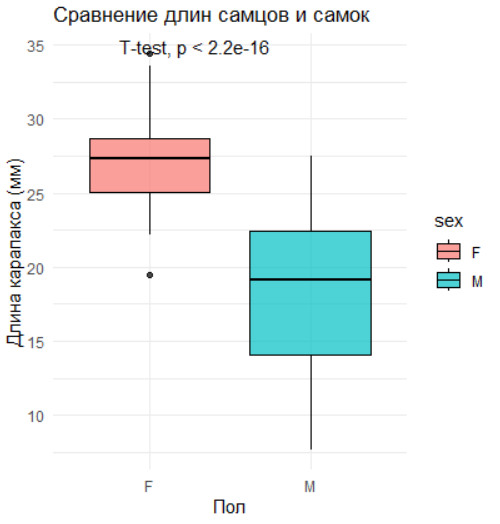
\includegraphics[width=0.6\linewidth,height=\textheight,keepaspectratio]{images/ttest_shrimp.PNG}

}

\caption{Рис. 1.10: Boxplot сравнения длин самцов и самок}

\end{figure}%

\subsubsection{\texorpdfstring{\textbf{Интерпретация
результатов}}{Интерпретация результатов}}\label{ux438ux43dux442ux435ux440ux43fux440ux435ux442ux430ux446ux438ux44f-ux440ux435ux437ux443ux43bux44cux442ux430ux442ux43eux432}

\begin{enumerate}
\def\labelenumi{\arabic{enumi}.}
\item
  Если p-value \textless{} 0.05, различия между группами статистически
  значимы.
\item
  Эффект размера помогает оценить биологическую важность различий.
  Например, если самки значительно крупнее самцов (d = 1.2), это может
  указывать на половой диморфизм, связанный с репродуктивной стратегией.

  \subsubsection{\texorpdfstring{\textbf{Пример полного анализа для
  веса}}{Пример полного анализа для веса}}\label{ux43fux440ux438ux43cux435ux440-ux43fux43eux43bux43dux43eux433ux43e-ux430ux43dux430ux43bux438ux437ux430-ux434ux43bux44f-ux432ux435ux441ux430}
\end{enumerate}

\begin{Shaded}
\begin{Highlighting}[]
\CommentTok{\# Полный анализ для веса  }
\NormalTok{weight\_analysis }\OtherTok{\textless{}{-}}\NormalTok{ data }\SpecialCharTok{\%\textgreater{}\%}  
  \FunctionTok{group\_by}\NormalTok{(sex) }\SpecialCharTok{\%\textgreater{}\%}  
  \FunctionTok{summarise}\NormalTok{(  }
    \AttributeTok{mean\_weight =} \FunctionTok{mean}\NormalTok{(weight),  }
    \AttributeTok{sd\_weight =} \FunctionTok{sd}\NormalTok{(weight),  }
    \AttributeTok{n =} \FunctionTok{n}\NormalTok{()  }
\NormalTok{  ) }\SpecialCharTok{\%\textgreater{}\%}  
  \FunctionTok{mutate}\NormalTok{(  }
    \AttributeTok{t\_test =} \FunctionTok{list}\NormalTok{(}\FunctionTok{t\_test}\NormalTok{(weight }\SpecialCharTok{\textasciitilde{}}\NormalTok{ sex, }\AttributeTok{data =}\NormalTok{ data)),  }
    \AttributeTok{cohens\_d =} \FunctionTok{list}\NormalTok{(}\FunctionTok{cohens\_d}\NormalTok{(weight }\SpecialCharTok{\textasciitilde{}}\NormalTok{ sex, }\AttributeTok{data =}\NormalTok{ data))  }
\NormalTok{  )  }

\CommentTok{\# Вывод результатов  }
\FunctionTok{print}\NormalTok{(weight\_analysis) }

\CommentTok{\# Распределение веса по полу}
\FunctionTok{ggplot}\NormalTok{(data, }\FunctionTok{aes}\NormalTok{(}\AttributeTok{x =} \FunctionTok{factor}\NormalTok{(sex), }\AttributeTok{y =}\NormalTok{ weight, }\AttributeTok{fill =} \FunctionTok{factor}\NormalTok{(sex))) }\SpecialCharTok{+}
  \FunctionTok{geom\_violin}\NormalTok{(}\AttributeTok{trim =} \ConstantTok{FALSE}\NormalTok{, }\AttributeTok{alpha =} \FloatTok{0.7}\NormalTok{) }\SpecialCharTok{+}
  \FunctionTok{geom\_boxplot}\NormalTok{(}\AttributeTok{width =} \FloatTok{0.2}\NormalTok{, }\AttributeTok{outlier.shape =} \ConstantTok{NA}\NormalTok{, }\AttributeTok{fill =} \StringTok{"white"}\NormalTok{) }\SpecialCharTok{+}
  \FunctionTok{labs}\NormalTok{(}\AttributeTok{title =} \StringTok{"Распределение веса по полу"}\NormalTok{, }\AttributeTok{x =} \StringTok{"Пол"}\NormalTok{, }\AttributeTok{y =} \StringTok{"Вес (г)"}\NormalTok{) }\SpecialCharTok{+}
  \FunctionTok{theme\_minimal}\NormalTok{()}
\end{Highlighting}
\end{Shaded}

\begin{figure}[H]

{\centering 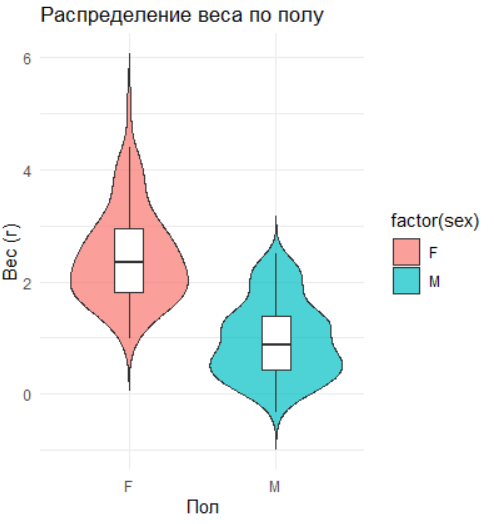
\includegraphics[width=0.6\linewidth,height=\textheight,keepaspectratio]{images/violin_shrimp.PNG}

}

\caption{Рис. 1.12: Violin plot для визуализации распределения веса}

\end{figure}%

\subsubsection{\texorpdfstring{\textbf{Выводы}}{Выводы}}\label{ux432ux44bux432ux43eux434ux44b}

\begin{enumerate}
\def\labelenumi{\arabic{enumi}.}
\item
  Используйте t-тест для нормальных данных и U-тест для ненормальных.
\item
  Дополните анализ оценкой эффекта размера для биологической
  интерпретации.
\item
  Визуализируйте различия с помощью boxplot или violin plot.
\end{enumerate}

\textbf{Рекомендации} :

\begin{itemize}
\item
  Для многомерных данных (например, одновременное сравнение длины, веса
  и возраста) применяйте MANOVA.
\item
  Если группы неоднородны (например, разный возрастной состав),
  используйте ковариационный анализ (ANCOVA).

  \subsection{\texorpdfstring{\textbf{Что делать, если тест на
  нормальность не пройден для одной из
  групп?}}{Что делать, если тест на нормальность не пройден для одной из групп?}}\label{ux447ux442ux43e-ux434ux435ux43bux430ux442ux44c-ux435ux441ux43bux438-ux442ux435ux441ux442-ux43dux430-ux43dux43eux440ux43cux430ux43bux44cux43dux43eux441ux442ux44c-ux43dux435-ux43fux440ux43eux439ux434ux435ux43d-ux434ux43bux44f-ux43eux434ux43dux43eux439-ux438ux437-ux433ux440ux443ux43fux43f}

  При сравнении количественных характеристик (например, длины карапакса
  у самцов и самок) важно учитывать, соответствуют ли данные нормальному
  распределению. Если тест на нормальность (например, Шапиро-Уилка)
  показывает значимое отклонение от нормальности для одной из групп, это
  влияет на выбор статистического теста и интерпретацию результатов.

  \subsubsection{\texorpdfstring{\textbf{Пример из нашего
  анализа}}{Пример из нашего анализа}}\label{ux43fux440ux438ux43cux435ux440-ux438ux437-ux43dux430ux448ux435ux433ux43e-ux430ux43dux430ux43bux438ux437ux430}

  Мы провели сравнение длины карапакса между самцами и самками:

  \begin{itemize}
  \item
    Для самцов: \textbf{\texttt{shapiro\_test(males\$length)}} → p-value
    = \textbf{0.000574} (нормальность отвергнута).
  \item
    Для самок: \textbf{\texttt{shapiro\_test(females\$length)}} →
    p-value = \textbf{0.891} (нормальность подтверждена).
  \end{itemize}

  Несмотря на это, мы применили как \textbf{t-тест} , так и
  \textbf{U-тест Манна-Уитни} :

  \begin{itemize}
  \item
    \textbf{t-тест} : p-value = 1.46e-40 (значимо).
  \item
    \textbf{U-тест} : p-value = 1.97e-27 (значимо).
  \item
    Коэффициент Коэна: d = 2.14 (большой эффект).
  \end{itemize}

  \subsubsection{\texorpdfstring{\textbf{Почему это
  работает?}}{Почему это работает?}}\label{ux43fux43eux447ux435ux43cux443-ux44dux442ux43e-ux440ux430ux431ux43eux442ux430ux435ux442}

  \begin{enumerate}
  \def\labelenumi{\arabic{enumi}.}
  \item
    \textbf{t-тест устойчив к умеренным отклонениям от нормальности} :

    \begin{itemize}
    \item
      При больших выборках (n \textgreater{} 30) центральная предельная
      теорема позволяет использовать t-тест даже при слабо выраженной
      асимметрии.
    \item
      В вашем случае выборка самцов (n = 149) достаточно велика, чтобы
      компенсировать отклонение от нормальности.
    \end{itemize}
  \item
    \textbf{U-тест Манна-Уитни --- непараметрическая альтернатива} :

    \begin{itemize}
    \item
      Этот тест не требует нормальности и сравнивает ранги, а не средние
      значения.
    \item
      Он подтверждает значимость различий, что усиливает доверие к
      выводу.
    \end{itemize}
  \item
    \textbf{Эффект размера (коэффициент Кобена)} :

    \begin{itemize}
    \tightlist
    \item
      d = 2.14 указывает на \textbf{большой эффект} , что важно для
      биологической интерпретации, даже если p-values значимы.
    \end{itemize}
  \end{enumerate}
\end{itemize}

\subsection{Сравнение параметров (линейные модели для оценки
межгрупповых
различий)}\label{ux441ux440ux430ux432ux43dux435ux43dux438ux435-ux43fux430ux440ux430ux43cux435ux442ux440ux43eux432-ux43bux438ux43dux435ux439ux43dux44bux435-ux43cux43eux434ux435ux43bux438-ux434ux43bux44f-ux43eux446ux435ux43dux43aux438-ux43cux435ux436ux433ux440ux443ux43fux43fux43eux432ux44bux445-ux440ux430ux437ux43bux438ux447ux438ux439}

Для сравнения параметров двух линейных моделей (например, скорости роста
самцов и самок) используем следующий подход.

\begin{Shaded}
\begin{Highlighting}[]
\CommentTok{\# Установка рабочей директории}
\FunctionTok{setwd}\NormalTok{(}\StringTok{"C:/TEXTBOOK/"}\NormalTok{)}

\CommentTok{\# Загрузка библиотек}
\FunctionTok{library}\NormalTok{(tidyverse)}
\FunctionTok{library}\NormalTok{(ggplot2)}
\FunctionTok{library}\NormalTok{(broom)}
\FunctionTok{library}\NormalTok{(knitr)}

\CommentTok{\# Загрузка данных}
\NormalTok{data }\OtherTok{\textless{}{-}} \FunctionTok{read\_csv}\NormalTok{(}\StringTok{"shrimp\_catch.csv"}\NormalTok{) }\SpecialCharTok{\%\textgreater{}\%}
  \FunctionTok{filter}\NormalTok{(}\SpecialCharTok{!}\NormalTok{id }\SpecialCharTok{\%in\%} \FunctionTok{c}\NormalTok{(}\DecValTok{10}\NormalTok{, }\DecValTok{50}\NormalTok{))  }\CommentTok{\# Удаление аномальных наблюдений}

\CommentTok{\# Фильтрация данных по полу}
\NormalTok{data\_male }\OtherTok{\textless{}{-}}\NormalTok{ data }\SpecialCharTok{\%\textgreater{}\%} \FunctionTok{filter}\NormalTok{(sex }\SpecialCharTok{==} \StringTok{"M"}\NormalTok{)}
\NormalTok{data\_female }\OtherTok{\textless{}{-}}\NormalTok{ data }\SpecialCharTok{\%\textgreater{}\%} \FunctionTok{filter}\NormalTok{(sex }\SpecialCharTok{==} \StringTok{"F"}\NormalTok{)}

\CommentTok{\# Построение моделей}
\NormalTok{model\_male }\OtherTok{\textless{}{-}} \FunctionTok{lm}\NormalTok{(length }\SpecialCharTok{\textasciitilde{}}\NormalTok{ age, }\AttributeTok{data =}\NormalTok{ data\_male)}
\NormalTok{model\_female }\OtherTok{\textless{}{-}} \FunctionTok{lm}\NormalTok{(length }\SpecialCharTok{\textasciitilde{}}\NormalTok{ age, }\AttributeTok{data =}\NormalTok{ data\_female)}

\FunctionTok{ggplot}\NormalTok{(data, }\FunctionTok{aes}\NormalTok{(age, length, }\AttributeTok{color =}\NormalTok{ sex)) }\SpecialCharTok{+}
  \FunctionTok{geom\_point}\NormalTok{(}\AttributeTok{alpha =} \FloatTok{0.5}\NormalTok{) }\SpecialCharTok{+}
  \FunctionTok{geom\_smooth}\NormalTok{(}\AttributeTok{method =} \StringTok{"lm"}\NormalTok{, }\AttributeTok{formula =}\NormalTok{ y }\SpecialCharTok{\textasciitilde{}}\NormalTok{ x) }\SpecialCharTok{+}
  \FunctionTok{scale\_color\_manual}\NormalTok{(}\AttributeTok{values =} \FunctionTok{c}\NormalTok{(}\StringTok{"\#E7B800"}\NormalTok{, }\StringTok{"\#00AFBB"}\NormalTok{)) }\SpecialCharTok{+}
  \FunctionTok{labs}\NormalTok{(}\AttributeTok{x =} \StringTok{"Возраст"}\NormalTok{, }\AttributeTok{y =} \StringTok{"Длина (мм)"}\NormalTok{) }\SpecialCharTok{+}
  \FunctionTok{theme\_minimal}\NormalTok{()}
\end{Highlighting}
\end{Shaded}

\begin{figure}[H]

{\centering 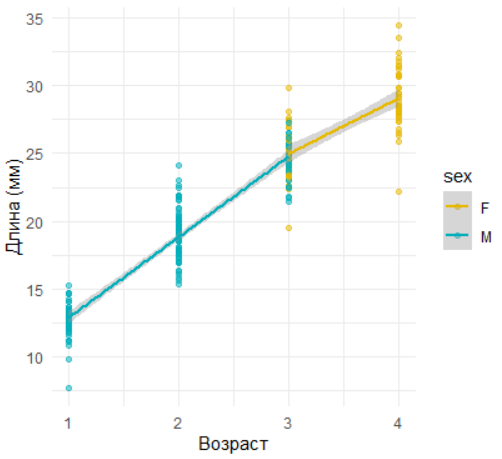
\includegraphics[width=0.6\linewidth,height=\textheight,keepaspectratio]{images/comparison_shrimp.PNG}

}

\caption{Рис. 1.15: Визуализация моделей}

\end{figure}%

\textbf{Метод 1: Объединенная модель с взаимодействиями}

\begin{Shaded}
\begin{Highlighting}[]
\CommentTok{\# Установка рабочей директории}
\NormalTok{joint\_model }\OtherTok{\textless{}{-}} \FunctionTok{lm}\NormalTok{(length }\SpecialCharTok{\textasciitilde{}}\NormalTok{ age }\SpecialCharTok{*}\NormalTok{ sex, }\AttributeTok{data =}\NormalTok{ data)}
\FunctionTok{summary}\NormalTok{(joint\_model) }\SpecialCharTok{\%\textgreater{}\%} 
\NormalTok{  broom}\SpecialCharTok{::}\FunctionTok{tidy}\NormalTok{() }\SpecialCharTok{\%\textgreater{}\%} 
  \FunctionTok{filter}\NormalTok{(term }\SpecialCharTok{==} \StringTok{"age:sexM"}\NormalTok{) }\SpecialCharTok{\%\textgreater{}\%} 
  \FunctionTok{kable}\NormalTok{(}\AttributeTok{caption =} \StringTok{"Проверка различия наклонов"}\NormalTok{, }\AttributeTok{digits =} \DecValTok{3}\NormalTok{)}
\end{Highlighting}
\end{Shaded}

\begin{Shaded}
\begin{Highlighting}[]
\NormalTok{Table}\SpecialCharTok{:}\NormalTok{ Проверка различия наклонов}

\SpecialCharTok{|}\NormalTok{term     }\SpecialCharTok{|}\NormalTok{ estimate}\SpecialCharTok{|}\NormalTok{ std.error}\SpecialCharTok{|}\NormalTok{ statistic}\SpecialCharTok{|}\NormalTok{ p.value}\SpecialCharTok{|}
\ErrorTok{|:}\SpecialCharTok{{-}{-}{-}{-}{-}{-}{-}{-}}\ErrorTok{|}\SpecialCharTok{{-}{-}{-}{-}{-}{-}{-}{-}}\ErrorTok{:|}\SpecialCharTok{{-}{-}{-}{-}{-}{-}{-}{-}{-}}\ErrorTok{:|}\SpecialCharTok{{-}{-}{-}{-}{-}{-}{-}{-}{-}}\ErrorTok{:|}\SpecialCharTok{{-}{-}{-}{-}{-}{-}{-}}\ErrorTok{:|}
\ErrorTok{|}\NormalTok{age}\SpecialCharTok{:}\NormalTok{sexM }\SpecialCharTok{|}     \FloatTok{1.86}\SpecialCharTok{|}     \FloatTok{0.459}\SpecialCharTok{|}     \FloatTok{4.053}\SpecialCharTok{|}       \DecValTok{0}\SpecialCharTok{|}
\ErrorTok{\textgreater{}} 
\end{Highlighting}
\end{Shaded}

\textbf{Интерпретация:}\\
Значимый коэффициент взаимодействия \textbf{\texttt{age:sexM}} (p
\textless{} 0.05) указывает на статистически значимые различия в
скорости роста между полами.

\textbf{Метод 2: Тест Вальда}

\begin{Shaded}
\begin{Highlighting}[]
\FunctionTok{library}\NormalTok{(car)}
\NormalTok{delta\_beta }\OtherTok{\textless{}{-}} \FunctionTok{coef}\NormalTok{(model\_male)[}\StringTok{"age"}\NormalTok{] }\SpecialCharTok{{-}} \FunctionTok{coef}\NormalTok{(model\_female)[}\StringTok{"age"}\NormalTok{]}
\NormalTok{se\_diff }\OtherTok{\textless{}{-}} \FunctionTok{sqrt}\NormalTok{(}\FunctionTok{vcov}\NormalTok{(model\_male)[}\StringTok{"age"}\NormalTok{,}\StringTok{"age"}\NormalTok{] }\SpecialCharTok{+} \FunctionTok{vcov}\NormalTok{(model\_female)[}\StringTok{"age"}\NormalTok{,}\StringTok{"age"}\NormalTok{])}
\NormalTok{z\_score }\OtherTok{\textless{}{-}}\NormalTok{ delta\_beta }\SpecialCharTok{/}\NormalTok{ se\_diff}
\NormalTok{p\_value }\OtherTok{\textless{}{-}} \DecValTok{2} \SpecialCharTok{*} \FunctionTok{pnorm}\NormalTok{(}\SpecialCharTok{{-}}\FunctionTok{abs}\NormalTok{(z\_score))}

\FunctionTok{cat}\NormalTok{(}\StringTok{"Разница коэффициентов:"}\NormalTok{, }\FunctionTok{round}\NormalTok{(delta\_beta, }\DecValTok{3}\NormalTok{), }
    \StringTok{"}\SpecialCharTok{\textbackslash{}n}\StringTok{Z{-}статистика:"}\NormalTok{, }\FunctionTok{round}\NormalTok{(z\_score, }\DecValTok{3}\NormalTok{),}
    \StringTok{"}\SpecialCharTok{\textbackslash{}n}\StringTok{p{-}value:"}\NormalTok{, }\FunctionTok{format.pval}\NormalTok{(p\_value, }\AttributeTok{digits =} \DecValTok{2}\NormalTok{))}


\NormalTok{comparison\_table }\OtherTok{\textless{}{-}} \FunctionTok{data.frame}\NormalTok{(}
\NormalTok{  Параметр }\OtherTok{=} \FunctionTok{c}\NormalTok{(}\StringTok{"Скорость роста самцов"}\NormalTok{, }\StringTok{"Скорость роста самок"}\NormalTok{, }\StringTok{"Разница"}\NormalTok{),}
\NormalTok{  Значение }\OtherTok{=} \FunctionTok{c}\NormalTok{(}
    \FunctionTok{round}\NormalTok{(}\FunctionTok{coef}\NormalTok{(model\_male)[}\StringTok{"age"}\NormalTok{], }\DecValTok{2}\NormalTok{),}
    \FunctionTok{round}\NormalTok{(}\FunctionTok{coef}\NormalTok{(model\_female)[}\StringTok{"age"}\NormalTok{], }\DecValTok{2}\NormalTok{),}
    \FunctionTok{round}\NormalTok{(delta\_beta, }\DecValTok{2}\NormalTok{)}
\NormalTok{  ),}
  \StringTok{\textasciigrave{}}\AttributeTok{p{-}value}\StringTok{\textasciigrave{}} \OtherTok{=} \FunctionTok{c}\NormalTok{(}
    \FunctionTok{format.pval}\NormalTok{(}\FunctionTok{summary}\NormalTok{(model\_male)}\SpecialCharTok{$}\NormalTok{coefficients[}\StringTok{"age"}\NormalTok{,}\DecValTok{4}\NormalTok{], }\AttributeTok{digits =} \DecValTok{2}\NormalTok{),}
    \FunctionTok{format.pval}\NormalTok{(}\FunctionTok{summary}\NormalTok{(model\_female)}\SpecialCharTok{$}\NormalTok{coefficients[}\StringTok{"age"}\NormalTok{,}\DecValTok{4}\NormalTok{], }\AttributeTok{digits =} \DecValTok{2}\NormalTok{),}
    \FunctionTok{format.pval}\NormalTok{(p\_value, }\AttributeTok{digits =} \DecValTok{2}\NormalTok{)}
\NormalTok{  )}
\NormalTok{)}
\FunctionTok{kable}\NormalTok{(comparison\_table, }\AttributeTok{caption =} \StringTok{"Сравнение коэффициентов роста"}\NormalTok{)}
\end{Highlighting}
\end{Shaded}

Вывод

\begin{Shaded}
\begin{Highlighting}[]
\SpecialCharTok{:}\NormalTok{ Сравнение коэффициентов роста}

\SpecialCharTok{|}\NormalTok{Параметр              }\SpecialCharTok{|}\NormalTok{ Значение}\SpecialCharTok{|}\NormalTok{p.value }\SpecialCharTok{|}
\ErrorTok{|:}\SpecialCharTok{{-}{-}{-}{-}{-}{-}{-}{-}{-}{-}{-}{-}{-}{-}{-}{-}{-}{-}{-}{-}{-}}\ErrorTok{|}\SpecialCharTok{{-}{-}{-}{-}{-}{-}{-}{-}}\ErrorTok{:|:}\SpecialCharTok{{-}{-}{-}{-}{-}{-}{-}}\ErrorTok{|}
\ErrorTok{|}\NormalTok{Скорость роста самцов }\SpecialCharTok{|}     \FloatTok{5.95}\SpecialCharTok{|}\ErrorTok{\textless{}}\FloatTok{2e{-}16}  \SpecialCharTok{|}
\ErrorTok{|}\NormalTok{Скорость роста самок  }\SpecialCharTok{|}     \FloatTok{4.09}\SpecialCharTok{|}\FloatTok{5.2e{-}13} \SpecialCharTok{|}
\ErrorTok{|}\NormalTok{Разница               }\SpecialCharTok{|}     \FloatTok{1.86}\SpecialCharTok{|}\FloatTok{0.00024} \SpecialCharTok{|}
\ErrorTok{\textgreater{}} 
\end{Highlighting}
\end{Shaded}

\textbf{Интерпретация:}\\
Значимая \emph{разница} (p \textless{} 0.05) указывает на статистически
значимые различия в скорости роста между полами.

\subsection{Сравнение
моделей}\label{ux441ux440ux430ux432ux43dux435ux43dux438ux435-ux43cux43eux434ux435ux43bux435ux439}

Одним из ключевых аспектов анализа биологических данных является
определение формы зависимости между переменными. В данном разделе мы
рассмотрим основы подбора модели зависимости между длиной и весом
креветок. Начиная с простой линейной модели, мы постепенно перейдем к
более сложным нелинейным моделям, чтобы продемонстрировать методику
выбора наилучшей модели. Cравним три модели --- линейную, полиномиальную
и степенную --- чтобы определить, какая из них наилучшим образом
описывает данные. Цель анализа --- найти математическую зависимость,
которая:

\begin{enumerate}
\def\labelenumi{\arabic{enumi}.}
\item
  Точно предсказывает вес креветки по её длине.
\item
  Имеет биологическую интерпретацию.
\item
  Минимизирует ошибку предсказания.
\end{enumerate}

\subsubsection{Модели и их
параметры}\label{ux43cux43eux434ux435ux43bux438-ux438-ux438ux445-ux43fux430ux440ux430ux43cux435ux442ux440ux44b}

\begin{enumerate}
\def\labelenumi{\arabic{enumi}.}
\tightlist
\item
  \textbf{Линейная}:
  \(\text{weight} = \beta_0 + \beta_1\cdot\text{length}\)
\item
  \textbf{Полиномиальная 3-й степени}:
  \(\text{weight} = \beta_0 + \beta_1\cdot\text{length} + \beta_2\cdot\text{length}^2 + \beta_3\cdot\text{length}^3\)
\item
  \textbf{Степенная}: \(\text{weight} = a\cdot\text{length}^b\)
\end{enumerate}

\subsubsection{Метрики}\label{ux43cux435ux442ux440ux438ux43aux438}

\begin{itemize}
\tightlist
\item
  \textbf{R²} - (коэффициент детерминации): чем ближе к 1, тем лучше
  модель объясняет данные.
\item
  \textbf{AIC} -(информационный критерий Акаике): чем меньше значение,
  тем лучше модель с учётом её сложности.
\end{itemize}

\subsubsection{\texorpdfstring{\textbf{Результаты}}{Результаты}}\label{ux440ux435ux437ux443ux43bux44cux442ux430ux442ux44b}

\paragraph{\texorpdfstring{\textbf{1. Линейная
модель}}{1. Линейная модель}}\label{ux43bux438ux43dux435ux439ux43dux430ux44f-ux43cux43eux434ux435ux43bux44c}

\begin{Shaded}
\begin{Highlighting}[]
\NormalTok{Coefficients}\SpecialCharTok{:}
\NormalTok{             Estimate Std. Error t value }\FunctionTok{Pr}\NormalTok{(}\SpecialCharTok{\textgreater{}}\ErrorTok{|}\NormalTok{t}\SpecialCharTok{|}\NormalTok{)    }
\NormalTok{(Intercept) }\SpecialCharTok{{-}}\FloatTok{2.115}      \FloatTok{0.085}     \SpecialCharTok{{-}}\FloatTok{24.86}   \SpecialCharTok{\textless{}}\FloatTok{2e{-}16} \SpecialCharTok{**}\ErrorTok{*}
\NormalTok{length       }\FloatTok{0.1665}     \FloatTok{0.0038}    \FloatTok{43.71}    \SpecialCharTok{\textless{}}\FloatTok{2e{-}16} \SpecialCharTok{**}\ErrorTok{*}
\end{Highlighting}
\end{Shaded}

\begin{itemize}
\item
  \textbf{R² = 0.894}
\item
  \textbf{AIC = 148.02}
\end{itemize}

\begin{figure}[H]

{\centering 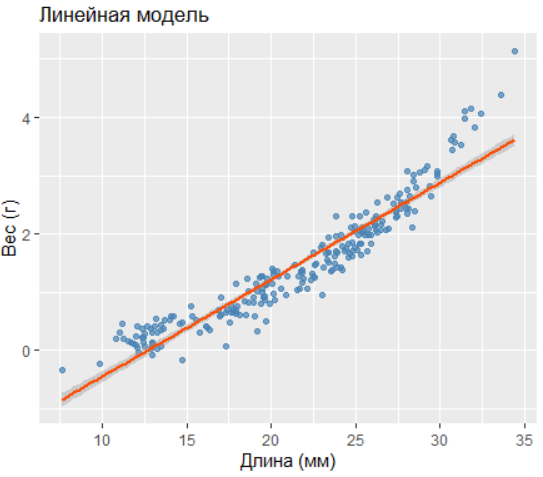
\includegraphics[width=0.6\linewidth,height=\textheight,keepaspectratio]{images/linear_shrimp.PNG}

}

\caption{Рис. 1.5: Линейная модель}

\end{figure}%

\paragraph{\texorpdfstring{\textbf{2. Полиномиальная
модель}}{2. Полиномиальная модель}}\label{ux43fux43eux43bux438ux43dux43eux43cux438ux430ux43bux44cux43dux430ux44f-ux43cux43eux434ux435ux43bux44c}

\begin{Shaded}
\begin{Highlighting}[]
\NormalTok{Coefficients}\SpecialCharTok{:}
\NormalTok{                 Estimate Std. Error t value }\FunctionTok{Pr}\NormalTok{(}\SpecialCharTok{\textgreater{}}\ErrorTok{|}\NormalTok{t}\SpecialCharTok{|}\NormalTok{)    }
\FunctionTok{poly}\NormalTok{(length,}\DecValTok{3}\NormalTok{)}\DecValTok{1}  \FloatTok{14.5038}    \FloatTok{0.2127}    \FloatTok{68.18}   \SpecialCharTok{\textless{}}\FloatTok{2e{-}16} \SpecialCharTok{**}\ErrorTok{*}
\FunctionTok{poly}\NormalTok{(length,}\DecValTok{3}\NormalTok{)}\DecValTok{2}   \FloatTok{3.7209}    \FloatTok{0.2127}    \FloatTok{17.49}   \SpecialCharTok{\textless{}}\FloatTok{2e{-}16} \SpecialCharTok{**}\ErrorTok{*}
\FunctionTok{poly}\NormalTok{(length,}\DecValTok{3}\NormalTok{)}\DecValTok{3}   \FloatTok{0.9526}    \FloatTok{0.2127}     \FloatTok{4.48}  \FloatTok{1.2e{-}05} \SpecialCharTok{**}\ErrorTok{*}
\end{Highlighting}
\end{Shaded}

\begin{itemize}
\item
  \textbf{R² = 0.957}
\item
  \textbf{AIC = -52.80}
\end{itemize}

\begin{figure}[H]

{\centering 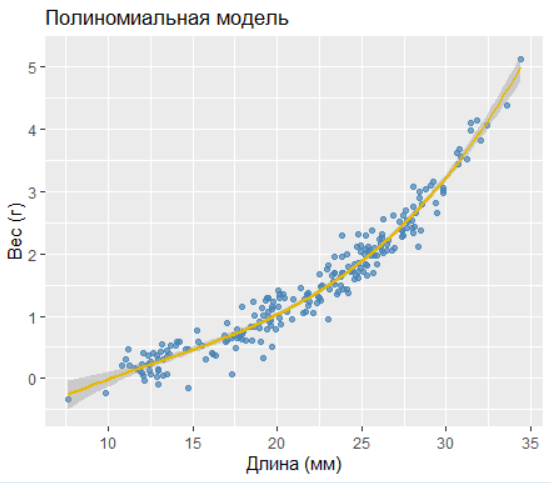
\includegraphics[width=0.6\linewidth,height=\textheight,keepaspectratio]{images/poly_shrimp.PNG}

}

\caption{Рис. 1.5: Полиномиальная модель}

\end{figure}%

\paragraph{\texorpdfstring{\textbf{3. Степенная
модель}}{3. Степенная модель}}\label{ux441ux442ux435ux43fux435ux43dux43dux430ux44f-ux43cux43eux434ux435ux43bux44c}

\begin{Shaded}
\begin{Highlighting}[]
\NormalTok{Parameters}\SpecialCharTok{:}
\NormalTok{   Estimate Std. Error t value }\FunctionTok{Pr}\NormalTok{(}\SpecialCharTok{\textgreater{}}\ErrorTok{|}\NormalTok{t}\SpecialCharTok{|}\NormalTok{)    }
\NormalTok{a }\FloatTok{0.000157}   \FloatTok{0.000028}    \FloatTok{5.60}  \FloatTok{6.3e{-}08} \SpecialCharTok{**}\ErrorTok{*}
\NormalTok{b }\FloatTok{2.920160}   \FloatTok{0.054102}   \FloatTok{53.98}   \SpecialCharTok{\textless{}}\FloatTok{2e{-}16} \SpecialCharTok{**}\ErrorTok{*}
\end{Highlighting}
\end{Shaded}

\begin{itemize}
\item
  \textbf{R² = 0.955}
\item
  \textbf{AIC = -48.43} \begin{center}
  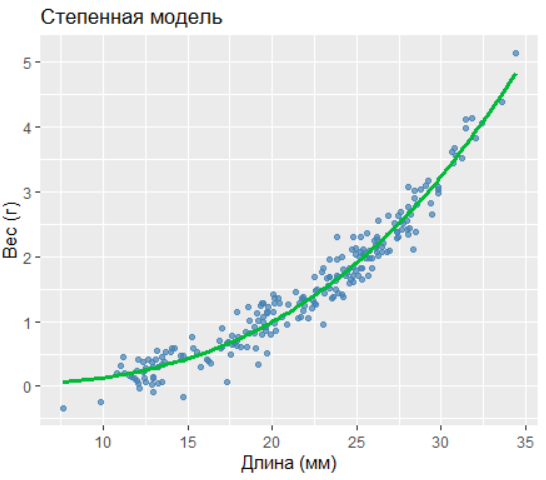
\includegraphics[width=0.6\linewidth,height=\textheight,keepaspectratio]{images/power_shrimp.PNG}
  \end{center}
\end{itemize}

\subsubsection{\texorpdfstring{\textbf{3. Сравнение
моделей}}{3. Сравнение моделей}}\label{ux441ux440ux430ux432ux43dux435ux43dux438ux435-ux43cux43eux434ux435ux43bux435ux439-1}

\begin{longtable}[]{@{}lll@{}}
\toprule\noalign{}
\textbf{Модель} & \textbf{R²} & \textbf{AIC} \\
\midrule\noalign{}
\endhead
\bottomrule\noalign{}
\endlastfoot
Линейная & 0.894 & 148.02 \\
Полиномиальная & 0.957 & -52.80 \\
Степенная & 0.955 & -48.43 \\
\end{longtable}

\textbf{Выводы:}

\begin{enumerate}
\def\labelenumi{\arabic{enumi}.}
\item
  \textbf{Полиномиальная модель} демонстрирует наилучшие показатели
  (максимальный R² и минимальный AIC).
\item
  \textbf{Степенная модель} близка по качеству, но её параметр
  \emph{b}≈2.92 близок к биологически ожидаемому значению 3 (вес
  пропорционален объёму).
\item
  \textbf{Линейная модель} существенно уступает по точности.
\end{enumerate}

\subsubsection{\texorpdfstring{\textbf{4.
Рекомендации}}{4. Рекомендации}}\label{ux440ux435ux43aux43eux43cux435ux43dux434ux430ux446ux438ux438}

\begin{itemize}
\item
  \textbf{Для прогнозирования} используйте полиномиальную модель, так
  как она минимизирует ошибку.
\item
  \textbf{Для биологической интерпретации} предпочтительна степенная
  модель: weight∝length\textsuperscript{2.92}.
\item
  \textbf{Избегайте переобучения:} Полиномиальные модели высокой степени
  могут терять интерпретируемость.
\end{itemize}

\subsubsection{\texorpdfstring{\textbf{5. Визуализация
остатков}}{5. Визуализация остатков}}\label{ux432ux438ux437ux443ux430ux43bux438ux437ux430ux446ux438ux44f-ux43eux441ux442ux430ux442ux43aux43eux432}

Остатки степенной модели распределены равномерно, что подтверждает её
адекватность: \begin{center}
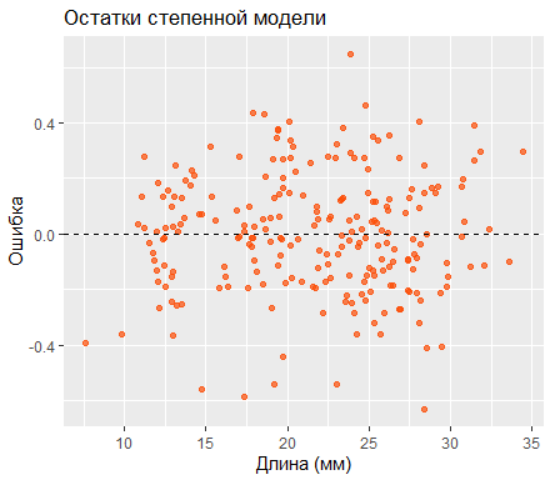
\includegraphics[width=0.6\linewidth,height=\textheight,keepaspectratio]{images/residuals_shrimp.PNG}
\end{center}

\subsubsection{\texorpdfstring{\textbf{Заключение}}{Заключение}}\label{ux437ux430ux43aux43bux44eux447ux435ux43dux438ux435}

Для анализа зависимости веса от длины северной креветки
\textbf{рекомендуется}:

\begin{enumerate}
\def\labelenumi{\arabic{enumi}.}
\item
  \textbf{Полиномиальная модель} --- для задач, требующих максимальной
  точности.
\item
  \textbf{Степенная модель} --- для интерпретации биологических
  закономерностей.
\end{enumerate}

Скрипт вышеописанных событий:

\begin{Shaded}
\begin{Highlighting}[]
\CommentTok{\# Установка рабочей директории}
\FunctionTok{setwd}\NormalTok{(}\StringTok{"C:/TEXTBOOK/"}\NormalTok{)}

\CommentTok{\# Загрузка библиотек}
\FunctionTok{library}\NormalTok{(tidyverse)}
\FunctionTok{library}\NormalTok{(ggplot2)}

\CommentTok{\# Загрузка данных}
\NormalTok{data }\OtherTok{\textless{}{-}} \FunctionTok{read\_csv}\NormalTok{(}\StringTok{"shrimp\_catch.csv"}\NormalTok{) }\SpecialCharTok{\%\textgreater{}\%}
  \FunctionTok{filter}\NormalTok{(}\SpecialCharTok{!}\NormalTok{id }\SpecialCharTok{\%in\%} \FunctionTok{c}\NormalTok{(}\DecValTok{10}\NormalTok{, }\DecValTok{50}\NormalTok{))  }\CommentTok{\# Удаление аномальных наблюдений}

\CommentTok{\# Проверка структуры}
\FunctionTok{glimpse}\NormalTok{(data)}

\CommentTok{\# Линейная модель: вес \textasciitilde{} длина}
\NormalTok{model\_linear }\OtherTok{\textless{}{-}} \FunctionTok{lm}\NormalTok{(weight }\SpecialCharTok{\textasciitilde{}}\NormalTok{ length, }\AttributeTok{data =}\NormalTok{ data)}
\FunctionTok{summary}\NormalTok{(model\_linear)}

\CommentTok{\# Визуализация}
\FunctionTok{ggplot}\NormalTok{(data, }\FunctionTok{aes}\NormalTok{(}\AttributeTok{x =}\NormalTok{ length, }\AttributeTok{y =}\NormalTok{ weight)) }\SpecialCharTok{+}
  \FunctionTok{geom\_point}\NormalTok{(}\AttributeTok{color =} \StringTok{"steelblue"}\NormalTok{, }\AttributeTok{alpha =} \FloatTok{0.7}\NormalTok{) }\SpecialCharTok{+}
  \FunctionTok{geom\_smooth}\NormalTok{(}\AttributeTok{method =} \StringTok{"lm"}\NormalTok{, }\AttributeTok{color =} \StringTok{"\#FC4E07"}\NormalTok{) }\SpecialCharTok{+}
  \FunctionTok{labs}\NormalTok{(}\AttributeTok{title =} \StringTok{"Линейная модель"}\NormalTok{, }\AttributeTok{x =} \StringTok{"Длина (мм)"}\NormalTok{, }\AttributeTok{y =} \StringTok{"Вес (г)"}\NormalTok{)}


\CommentTok{\# Полиномиальная модель: вес \textasciitilde{} длина + длина? + длина?}
\NormalTok{model\_poly }\OtherTok{\textless{}{-}} \FunctionTok{lm}\NormalTok{(weight }\SpecialCharTok{\textasciitilde{}} \FunctionTok{poly}\NormalTok{(length, }\DecValTok{3}\NormalTok{), }\AttributeTok{data =}\NormalTok{ data)}
\FunctionTok{summary}\NormalTok{(model\_poly)}

\CommentTok{\# Визуализация}
\FunctionTok{ggplot}\NormalTok{(data, }\FunctionTok{aes}\NormalTok{(}\AttributeTok{x =}\NormalTok{ length, }\AttributeTok{y =}\NormalTok{ weight)) }\SpecialCharTok{+}
  \FunctionTok{geom\_point}\NormalTok{(}\AttributeTok{color =} \StringTok{"steelblue"}\NormalTok{, }\AttributeTok{alpha =} \FloatTok{0.7}\NormalTok{) }\SpecialCharTok{+}
  \FunctionTok{geom\_smooth}\NormalTok{(}\AttributeTok{method =} \StringTok{"lm"}\NormalTok{, }\AttributeTok{formula =}\NormalTok{ y }\SpecialCharTok{\textasciitilde{}} \FunctionTok{poly}\NormalTok{(x, }\DecValTok{3}\NormalTok{), }\AttributeTok{color =} \StringTok{"\#E7B800"}\NormalTok{) }\SpecialCharTok{+}
  \FunctionTok{labs}\NormalTok{(}\AttributeTok{title =} \StringTok{"Полиномиальная модель"}\NormalTok{, }\AttributeTok{x =} \StringTok{"Длина (мм)"}\NormalTok{, }\AttributeTok{y =} \StringTok{"Вес (г)"}\NormalTok{)}


\CommentTok{\# Степенная модель: вес \textasciitilde{} длина\^{}k (k подбирается)}
\NormalTok{model\_power }\OtherTok{\textless{}{-}} \FunctionTok{nls}\NormalTok{(weight }\SpecialCharTok{\textasciitilde{}}\NormalTok{ a }\SpecialCharTok{*}\NormalTok{ length}\SpecialCharTok{\^{}}\NormalTok{b, }
                   \AttributeTok{data =}\NormalTok{ data, }
                   \AttributeTok{start =} \FunctionTok{list}\NormalTok{(}\AttributeTok{a =} \FloatTok{0.001}\NormalTok{, }\AttributeTok{b =} \DecValTok{3}\NormalTok{))  }\CommentTok{\# Начальные значения}
\FunctionTok{summary}\NormalTok{(model\_power)}

\CommentTok{\# Визуализация}
\NormalTok{data}\SpecialCharTok{$}\NormalTok{pred\_power }\OtherTok{\textless{}{-}} \FunctionTok{predict}\NormalTok{(model\_power)}
\FunctionTok{ggplot}\NormalTok{(data, }\FunctionTok{aes}\NormalTok{(}\AttributeTok{x =}\NormalTok{ length, }\AttributeTok{y =}\NormalTok{ weight)) }\SpecialCharTok{+}
  \FunctionTok{geom\_point}\NormalTok{(}\AttributeTok{color =} \StringTok{"steelblue"}\NormalTok{, }\AttributeTok{alpha =} \FloatTok{0.7}\NormalTok{) }\SpecialCharTok{+}
  \FunctionTok{geom\_line}\NormalTok{(}\FunctionTok{aes}\NormalTok{(}\AttributeTok{y =}\NormalTok{ pred\_power), }\AttributeTok{color =} \StringTok{"\#00BA38"}\NormalTok{, }\AttributeTok{linewidth =} \FloatTok{1.2}\NormalTok{) }\SpecialCharTok{+}
  \FunctionTok{labs}\NormalTok{(}\AttributeTok{title =} \StringTok{"Степенная модель"}\NormalTok{, }\AttributeTok{x =} \StringTok{"Длина (мм)"}\NormalTok{, }\AttributeTok{y =} \StringTok{"Вес (г)"}\NormalTok{)}

\CommentTok{\# Расчет AIC}
\FunctionTok{AIC}\NormalTok{(model\_linear, model\_poly, model\_power)}

\CommentTok{\# Расчет R?}
\NormalTok{r2\_linear }\OtherTok{\textless{}{-}} \FunctionTok{summary}\NormalTok{(model\_linear)}\SpecialCharTok{$}\NormalTok{r.squared}
\NormalTok{r2\_poly }\OtherTok{\textless{}{-}} \FunctionTok{summary}\NormalTok{(model\_poly)}\SpecialCharTok{$}\NormalTok{r.squared}
\NormalTok{r2\_power }\OtherTok{\textless{}{-}} \DecValTok{1} \SpecialCharTok{{-}} \FunctionTok{sum}\NormalTok{(}\FunctionTok{residuals}\NormalTok{(model\_power)}\SpecialCharTok{\^{}}\DecValTok{2}\NormalTok{) }\SpecialCharTok{/} \FunctionTok{sum}\NormalTok{((data}\SpecialCharTok{$}\NormalTok{weight }\SpecialCharTok{{-}} \FunctionTok{mean}\NormalTok{(data}\SpecialCharTok{$}\NormalTok{weight))}\SpecialCharTok{\^{}}\DecValTok{2}\NormalTok{)}

\CommentTok{\# Создание таблицы сравнения моделей}
\NormalTok{comparison\_table }\OtherTok{\textless{}{-}} \FunctionTok{data.frame}\NormalTok{(}
\NormalTok{  Модель }\OtherTok{=} \FunctionTok{c}\NormalTok{(}\StringTok{"Линейная"}\NormalTok{, }\StringTok{"Полиномиальная"}\NormalTok{, }\StringTok{"Степенная"}\NormalTok{),}
  \AttributeTok{R\_square =} \FunctionTok{c}\NormalTok{(r2\_linear, r2\_poly, r2\_power),}
  \AttributeTok{AIC =} \FunctionTok{c}\NormalTok{(}\FunctionTok{AIC}\NormalTok{(model\_linear), }\FunctionTok{AIC}\NormalTok{(model\_poly), }\FunctionTok{AIC}\NormalTok{(model\_power))}
\NormalTok{)}

\CommentTok{\# Вывод таблицы}
\FunctionTok{print}\NormalTok{(comparison\_table)}

\CommentTok{\# Остатки для степенной модели}
\NormalTok{data}\SpecialCharTok{$}\NormalTok{residuals }\OtherTok{\textless{}{-}} \FunctionTok{residuals}\NormalTok{(model\_power)}

\FunctionTok{ggplot}\NormalTok{(data, }\FunctionTok{aes}\NormalTok{(}\AttributeTok{x =}\NormalTok{ length, }\AttributeTok{y =}\NormalTok{ residuals)) }\SpecialCharTok{+}
  \FunctionTok{geom\_point}\NormalTok{(}\AttributeTok{color =} \StringTok{"\#FC4E07"}\NormalTok{, }\AttributeTok{alpha =} \FloatTok{0.7}\NormalTok{) }\SpecialCharTok{+}
  \FunctionTok{geom\_hline}\NormalTok{(}\AttributeTok{yintercept =} \DecValTok{0}\NormalTok{, }\AttributeTok{linetype =} \StringTok{"dashed"}\NormalTok{) }\SpecialCharTok{+}
  \FunctionTok{labs}\NormalTok{(}\AttributeTok{title =} \StringTok{"Остатки степенной модели"}\NormalTok{, }\AttributeTok{x =} \StringTok{"Длина (мм)"}\NormalTok{, }\AttributeTok{y =} \StringTok{"Ошибка"}\NormalTok{)}
\end{Highlighting}
\end{Shaded}

\bookmarksetup{startatroot}

\chapter{Нейронные сети в экологии: практическое
введение}\label{ux43dux435ux439ux440ux43eux43dux43dux44bux435-ux441ux435ux442ux438-ux432-ux44dux43aux43eux43bux43eux433ux438ux438-ux43fux440ux430ux43aux442ux438ux447ux435ux441ux43aux43eux435-ux432ux432ux435ux434ux435ux43dux438ux435}

\section{Введение}\label{ux432ux432ux435ux434ux435ux43dux438ux435-1}

Это практическое занятие можно рассматривать не только как введение в
нейронные сети, но и как введение в экологическое моделирование в общем
с помошью R. Занятие основано на статье Андрея Викторовича Коросова
``\href{https://ecopri.ru/journal/article.php?id=14002}{Нейронные сети в
экологии: введение}'', опубликованной в журнале Принципы экологии, №3,
2023, стр. 76-96. В статье рассмотрены основы нейросетевого
моделирования в экологии, начиная с классических регрессионных методов и
заканчивая искусственными нейронными сетями. Представленные примеры
демонстрируют эволюционный переход от простых линейных моделей к сложным
нейросетевым конструкциям, что позволяет решать задачи классификации и
прогнозирования в экологии. ``Теоретическая'' лекция, основанная на этой
статье, находиться по \href{KOROSOV.ppt}{ссылке}.

Можно скачать скрипт целиком в трех версиях:
\href{https://mombus.github.io/cRab/data/KOROSOV.R}{KOROSOV.R} -
максимально приближен к оригинальной работе;
\href{https://mombus.github.io/cRab/data/KOROSOV_updated.R}{KOROSOV\_updated.R}
- тотже скрипт, но с комментариями и пояснениями (содержание этого
занятия);
\href{https://mombus.github.io/cRab/data/KOROSOV_visual.R}{KOROSOV\_visual.R}
- почти такой же с дополнительным продвинутым визуалом и аналитикой.

\subsubsection{\texorpdfstring{\textbf{Для работы
скрипта:}}{Для работы скрипта:}}\label{ux434ux43bux44f-ux440ux430ux431ux43eux442ux44b-ux441ux43aux440ux438ux43fux442ux430}

\begin{enumerate}
\def\labelenumi{\arabic{enumi}.}
\item
  Скачайте файлы данных
  (\href{https://mombus.github.io/cRab/data/vipkar.csv}{vipkar.csv} и
  \href{https://mombus.github.io/cRab/data/kihzsdat.csv}{kihzsdat.csv})
\item
  Установите рабочую директорию в setwd()
\item
  Установите необходимые пакеты :
  \textbf{\texttt{install.packages(c("neuralnet",\ "ggplot2"))}}
\end{enumerate}

\begin{Shaded}
\begin{Highlighting}[]
\CommentTok{\# ЗАГРУЗКА БИБЛИОТЕК И НАСТРОЙКА СРЕДЫ ================================}
\FunctionTok{library}\NormalTok{(neuralnet)   }\CommentTok{\# Для построения нейронных сетей}
\FunctionTok{library}\NormalTok{(ggplot2)     }\CommentTok{\# Для продвинутой визуализации (в данном скрипте не используется напрямую)}

\CommentTok{\# Установите свою рабочую директорию (где лежат файлы данных)}
\CommentTok{\# setwd("C:/ВАША\_ДИРЕКТОРИЯ/")}
\end{Highlighting}
\end{Shaded}

\section{ЛИНЕЙНАЯ
РЕГРЕССИЯ}\label{ux43bux438ux43dux435ux439ux43dux430ux44f-ux440ux435ux433ux440ux435ux441ux441ux438ux44f}

В этом разделе мы изучим основы экологического моделирования на примере
зависимости массы тела гадюки от ее длины. Вы построите простую линейную
регрессионную модель, визуализируете данные и линию регрессии, а также
интерпретируете результаты с помощью функции \texttt{summary()}.

Загружаем данные

\begin{Shaded}
\begin{Highlighting}[]
\CommentTok{\# Данные: масса (w) и длина тела (lt) гадюк (в см и граммах)}
\NormalTok{w }\OtherTok{\textless{}{-}} \FunctionTok{c}\NormalTok{(}\DecValTok{85}\NormalTok{, }\DecValTok{90}\NormalTok{, }\DecValTok{85}\NormalTok{, }\DecValTok{95}\NormalTok{, }\DecValTok{95}\NormalTok{, }\DecValTok{135}\NormalTok{, }\DecValTok{165}\NormalTok{, }\DecValTok{135}\NormalTok{, }\DecValTok{140}\NormalTok{)}
\NormalTok{lt }\OtherTok{\textless{}{-}} \FunctionTok{c}\NormalTok{(}\DecValTok{51}\NormalTok{, }\DecValTok{51}\NormalTok{, }\DecValTok{52}\NormalTok{, }\DecValTok{54}\NormalTok{, }\DecValTok{54}\NormalTok{, }\DecValTok{59}\NormalTok{, }\DecValTok{59}\NormalTok{, }\DecValTok{60}\NormalTok{, }\DecValTok{62}\NormalTok{)}
\end{Highlighting}
\end{Shaded}

Строим и запускаем модель \[
w_t = a_0 + a_1 \cdot l_t
\]

где: - \(w_t\) --- зависимая переменная, - \(a_0\) --- свободный член, -
\(a_1\) --- коэффициент регрессии, - \(l_t\) --- независимая переменная.

\begin{Shaded}
\begin{Highlighting}[]
\CommentTok{\# Построение линейной модели: w = a0 + a1*lt}
\NormalTok{lreg }\OtherTok{\textless{}{-}} \FunctionTok{lm}\NormalTok{(w }\SpecialCharTok{\textasciitilde{}}\NormalTok{ lt)}
\end{Highlighting}
\end{Shaded}

Выведем результаты модели

\begin{Shaded}
\begin{Highlighting}[]
\CommentTok{\# Просмотр результатов модели:}
\FunctionTok{summary}\NormalTok{(lreg)  }\CommentTok{\# Обратите внимание на коэффициенты и p{-}значения}
\end{Highlighting}
\end{Shaded}

На экране появится:

\begin{Shaded}
\begin{Highlighting}[]
\NormalTok{Call}\SpecialCharTok{:}
\FunctionTok{lm}\NormalTok{(}\AttributeTok{formula =}\NormalTok{ w }\SpecialCharTok{\textasciitilde{}}\NormalTok{ lt)}

\NormalTok{Residuals}\SpecialCharTok{:}
\NormalTok{    Min      }\DecValTok{1}\NormalTok{Q  Median      }\DecValTok{3}\NormalTok{Q     Max }
\SpecialCharTok{{-}}\FloatTok{13.452}  \SpecialCharTok{{-}}\FloatTok{7.585}  \SpecialCharTok{{-}}\FloatTok{4.868}   \FloatTok{1.490}  \FloatTok{30.623} 

\NormalTok{Coefficients}\SpecialCharTok{:}
\NormalTok{            Estimate Std. Error t value }\FunctionTok{Pr}\NormalTok{(}\SpecialCharTok{\textgreater{}}\ErrorTok{|}\NormalTok{t}\SpecialCharTok{|}\NormalTok{)    }
\NormalTok{(Intercept) }\SpecialCharTok{{-}}\FloatTok{240.766}     \FloatTok{64.457}  \SpecialCharTok{{-}}\FloatTok{3.735} \FloatTok{0.007308} \SpecialCharTok{**} 
\NormalTok{lt             }\FloatTok{6.358}      \FloatTok{1.153}   \FloatTok{5.516} \FloatTok{0.000891} \SpecialCharTok{**}\ErrorTok{*}
\SpecialCharTok{{-}{-}{-}}
\NormalTok{Signif. codes}\SpecialCharTok{:}  \DecValTok{0}\NormalTok{ ‘}\SpecialCharTok{**}\ErrorTok{*}\NormalTok{’ }\FloatTok{0.001}\NormalTok{ ‘}\SpecialCharTok{**}\NormalTok{’ }\FloatTok{0.01}\NormalTok{ ‘}\SpecialCharTok{*}\NormalTok{’ }\FloatTok{0.05}\NormalTok{ ‘.’ }\FloatTok{0.1}\NormalTok{ ‘ ’ }\DecValTok{1}

\NormalTok{Residual standard error}\SpecialCharTok{:} \FloatTok{13.81}\NormalTok{ on }\DecValTok{7}\NormalTok{ degrees of freedom}
\NormalTok{Multiple R}\SpecialCharTok{{-}}\NormalTok{squared}\SpecialCharTok{:}  \FloatTok{0.813}\NormalTok{,     Adjusted R}\SpecialCharTok{{-}}\NormalTok{squared}\SpecialCharTok{:}  \FloatTok{0.7863} 
\NormalTok{F}\SpecialCharTok{{-}}\NormalTok{statistic}\SpecialCharTok{:} \FloatTok{30.43}\NormalTok{ on }\DecValTok{1}\NormalTok{ and }\DecValTok{7}\NormalTok{ DF,  p}\SpecialCharTok{{-}}\NormalTok{value}\SpecialCharTok{:} \FloatTok{0.0008911}
\end{Highlighting}
\end{Shaded}

Мы получили результаты линейной регрессии, где зависимая переменная ---
масса тела гадюки (w), а независимая переменная --- длина тела (lt).
Разберем каждый параметр:

1. **Call (Вызов модели):**

`lm(formula = w \textasciitilde{} lt)`

Это просто напоминание, какая модель была построена. Здесь указано, что
мы моделировали зависимость массы (w) от длины тела (lt) с помощью
линейной регрессии.

2. **Residuals (Остатки):**

Остатки --- это разница между наблюдаемыми значениями массы и
предсказанными моделью значениями. Они показывают, насколько хорошо
модель описывает данные.

\begin{itemize}
\item
  `Min`: минимальный остаток = -13.452 (наибольшее недооцененное
  значение)
\item
  `1Q`: первый квартиль = -7.585 (25\% остатков меньше этого значения)
\item
  `Median`: медиана остатков = -4.868 (середина распределения остатков)
\item
  `3Q`: третий квартиль = 1.490 (75\% остатков меньше этого значения)
\item
  `Max`: максимальный остаток = 30.623 (наибольшее переоцененное
  значение)
\end{itemize}

Распределение остатков: медиана немного смещена влево (отрицательное
значение), а размах между 1Q и 3Q составляет примерно 9 единиц. Это
может указывать на легкую асимметрию, но выборка мала.

3. **Coefficients (Коэффициенты):**

\begin{itemize}
\item
  `(Intercept)`: свободный член (a0) = -240.766. Это предсказанное
  значение массы при длине тела, равной нулю. Биологически это не имеет
  смысла (длина не может быть нулевой), но это математическая
  особенность модели.
\item
  `lt`: коэффициент регрессии (a1) = 6.358. Это означает, что при
  увеличении длины тела на 1 см масса тела увеличивается в среднем на
  6.358 г.
\end{itemize}

Для каждого коэффициента приведены:

\begin{itemize}
\item
  `Estimate`: точечная оценка коэффициента.
\item
  `Std. Error`: стандартная ошибка оценки коэффициента. Для intercept =
  64.457, для lt = 1.153. Это мера изменчивости оценки.
\item
  `t value`: t-статистика. Рассчитывается как Estimate / Std.Error. Для
  intercept: -240.766 / 64.457 ≈ -3.735; для lt: 6.358 / 1.153 ≈ 5.516.
\item
  `Pr(\textgreater\textbar t\textbar)`: p-значение для проверки гипотезы
  о равенстве коэффициента нулю.
\item
  Для intercept: p=0.007308 (значим на уровне α=0.01, т.е. intercept
  статистически значимо отличается от нуля).
\item
  Для lt: p=0.000891 (значим на уровне α=0.001). Это означает, что длина
  тела значимо влияет на массу.
\end{itemize}

Значимость кодов: три звездочки (`***`) означают, что коэффициент значим
на уровне 0.001.

4. **Residual standard error (Стандартная ошибка остатков):** 13.81 на 7
степенях свободы. Это мера разброса остатков. В среднем, предсказания
модели отклоняются от реальных значений на ±13.81 г. Степени свободы
(df) = n - 2 = 9 - 2 = 7 (n --- количество наблюдений).

5. **Multiple R-squared (Коэффициент детерминации R²):** 0.813. Это
означает, что 81.3\% вариации массы тела объясняется длиной тела.
Остальные 18.7\% --- это неучтенные факторы и случайная изменчивость.

6. **Adjusted R-squared (Скорректированный R²):** 0.7863. Этот
показатель корректирует R² с учетом числа предикторов. Он полезен при
сравнении моделей с разным числом предикторов. Здесь он немного меньше
R², так как учитывает, что в модели один предиктор.

7. **F-statistic (F-статистика):** 30.43 на 1 и 7 степенях свободы.
Проверяет гипотезу о том, что все коэффициенты (кроме intercept) равны
нулю (т.е. модель не лучше, чем модель только с константой).

\begin{itemize}
\tightlist
\item
  p-value: 0.0008911 (крайне значимый), что означает, что модель в целом
  адекватна.
\end{itemize}

**Выводы:**

- Уравнение модели: `w = -240.77 + 6.36 * lt`

- Длина тела значимо влияет на массу (p\textless0.001).

- Модель объясняет 81.3\% вариации массы.

- На каждый сантиметр длины тела масса увеличивается примерно на 6.36 г.

- Остатки модели показывают, что есть несколько точек, которые модель
предсказывает с заметной ошибкой (особенно максимальный остаток в 30.6
г). Возможно, для более точного прогноза нужна нелинейная модель или
учет дополнительных факторов.

**Рекомендации:**

- Проверить допущения линейной регрессии (нормальность остатков,
гомоскедастичность) с помощью диагностических графиков.

- Рассмотреть возможность включения других переменных (например,
возраста, пола) в модель.

- Убедиться, что в данных нет выбросов, которые могут влиять на
коэффициенты.

\begin{Shaded}
\begin{Highlighting}[]
\CommentTok{\# Визуализация зависимости}
\FunctionTok{plot}\NormalTok{(lt, w, }
     \AttributeTok{main =} \StringTok{"Зависимость массы от длины тела гадюки"}\NormalTok{, }
     \AttributeTok{xlab =} \StringTok{"Длина тела (см)"}\NormalTok{, }
     \AttributeTok{ylab =} \StringTok{"Масса (г)"}\NormalTok{, }
     \AttributeTok{pch =} \DecValTok{19}\NormalTok{,        }\CommentTok{\# Кружки вместо стандартных точек}
     \AttributeTok{col =} \StringTok{"darkgreen"}\NormalTok{)}
\FunctionTok{abline}\NormalTok{(lreg, }\AttributeTok{col =} \StringTok{"red"}\NormalTok{, }\AttributeTok{lwd =} \DecValTok{2}\NormalTok{)  }\CommentTok{\# Добавляем линию регрессии}
\end{Highlighting}
\end{Shaded}

\begin{figure}[H]

{\centering 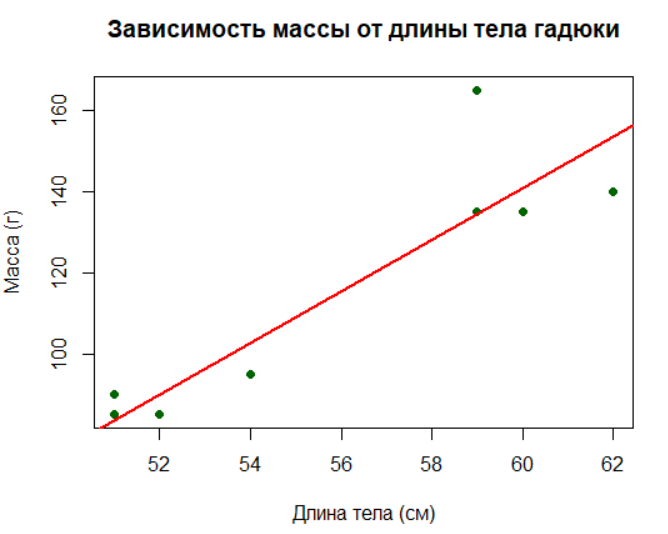
\includegraphics[width=0.6\linewidth,height=\textheight,keepaspectratio]{images/KOROSOV1.PNG}

}

\caption{Рис. 1.: Пример линейной регрессии}

\end{figure}%

\section{ЧИСЛЕННАЯ
ОПТИМИЗАЦИЯ}\label{ux447ux438ux441ux43bux435ux43dux43dux430ux44f-ux43eux43fux442ux438ux43cux438ux437ux430ux446ux438ux44f}

Здесь вы познакомитесь с численными методами оптимизации параметров
моделей, которые применяются, когда аналитическое решение невозможно. На
примере той же зависимости массы от длины вы подгоните параметры модели
с помощью функции \texttt{nls()} и сравните результаты с аналитическим
решением.

Аналитические методы дают точное решение в виде математической формулы,
используя алгебраические преобразования и теоремы математического
анализа. Они идеальны для простых моделей, где существуют явные решения,
обеспечивая прозрачную интерпретацию параметров. В экологии такие методы
применимы для базовых зависимостей типа линейной регрессии. Численные
методы используются, когда аналитическое решение невозможно, и работают
через последовательные приближения, начиная со стартовых значений и
итеративно улучшая параметры модели. Они незаменимы для сложных
экологических моделей с нелинейными зависимостями, взаимодействиями
факторов и ``шумными'' полевыми данными, позволяя решать задачи,
недоступные для аналитических подходов.

\begin{Shaded}
\begin{Highlighting}[]
\CommentTok{\# Подгонка параметров через оптимизацию}
\NormalTok{nls\_model }\OtherTok{\textless{}{-}} \FunctionTok{nls}\NormalTok{(w }\SpecialCharTok{\textasciitilde{}}\NormalTok{ a0 }\SpecialCharTok{+}\NormalTok{ a1 }\SpecialCharTok{*}\NormalTok{ lt, }\AttributeTok{start =} \FunctionTok{list}\NormalTok{(}\AttributeTok{a0 =} \DecValTok{1}\NormalTok{, }\AttributeTok{a1 =} \DecValTok{1}\NormalTok{))}
\FunctionTok{summary}\NormalTok{(nls\_model)}
\end{Highlighting}
\end{Shaded}

На экране появится:

\begin{Shaded}
\begin{Highlighting}[]
\NormalTok{Formula}\SpecialCharTok{:}\NormalTok{ w }\SpecialCharTok{\textasciitilde{}}\NormalTok{ a0 }\SpecialCharTok{+}\NormalTok{ a1 }\SpecialCharTok{*}\NormalTok{ lt}

\NormalTok{Parameters}\SpecialCharTok{:}
\NormalTok{   Estimate Std. Error t value }\FunctionTok{Pr}\NormalTok{(}\SpecialCharTok{\textgreater{}}\ErrorTok{|}\NormalTok{t}\SpecialCharTok{|}\NormalTok{)    }
\NormalTok{a0 }\SpecialCharTok{{-}}\FloatTok{240.766}     \FloatTok{64.457}  \SpecialCharTok{{-}}\FloatTok{3.735} \FloatTok{0.007308} \SpecialCharTok{**} 
\NormalTok{a1    }\FloatTok{6.358}      \FloatTok{1.153}   \FloatTok{5.516} \FloatTok{0.000891} \SpecialCharTok{**}\ErrorTok{*}
\SpecialCharTok{{-}{-}{-}}
\NormalTok{Signif. codes}\SpecialCharTok{:}  \DecValTok{0}\NormalTok{ ‘}\SpecialCharTok{**}\ErrorTok{*}\NormalTok{’ }\FloatTok{0.001}\NormalTok{ ‘}\SpecialCharTok{**}\NormalTok{’ }\FloatTok{0.01}\NormalTok{ ‘}\SpecialCharTok{*}\NormalTok{’ }\FloatTok{0.05}\NormalTok{ ‘.’ }\FloatTok{0.1}\NormalTok{ ‘ ’ }\DecValTok{1}

\NormalTok{Residual standard error}\SpecialCharTok{:} \FloatTok{13.81}\NormalTok{ on }\DecValTok{7}\NormalTok{ degrees of freedom}

\NormalTok{Number of iterations to convergence}\SpecialCharTok{:} \DecValTok{1} 
\NormalTok{Achieved convergence tolerance}\SpecialCharTok{:} \FloatTok{3.247e{-}08}
\end{Highlighting}
\end{Shaded}

\subsection{\texorpdfstring{\textbf{Интерпретация результатов
модели}}{Интерпретация результатов модели}}\label{ux438ux43dux442ux435ux440ux43fux440ux435ux442ux430ux446ux438ux44f-ux440ux435ux437ux443ux43bux44cux442ux430ux442ux43eux432-ux43cux43eux434ux435ux43bux438}

Мы построили линейную модель зависимости массы гадюки (w) от длины её
тела (lt) по формуле:\\
\textbf{\texttt{w\ =\ a0\ +\ a1\ *\ lt}}

\textbf{Ключевые параметры модели:}

\begin{itemize}
\item
  \textbf{a0 (свободный член)}: -240.8 г\\
  Это теоретическая масса при нулевой длине тела. Отрицательное значение
  указывает, что модель не подходит для очень молодых особей.
\item
  \textbf{a1 (коэффициент при lt)}: 6.36 г/см\\
  Каждый дополнительный сантиметр длины тела увеличивает массу в среднем
  на 6.36 г.
\end{itemize}

\textbf{Точность и значимость:}

\begin{itemize}
\item
  Оба коэффициента \textbf{высоко значимы} (p \textless{} 0.01), что
  подтверждает реальность зависимости.
\item
  Стандартная ошибка для a1 составляет 1.15 г/см - это значит, что
  реальное значение, вероятно, находится между 5.2 и 7.5 г/см.
\item
  Модель хорошо сошлась за 1 шаг (итерацию), что говорит об удачном
  подборе параметров.
\end{itemize}

\textbf{Ошибка прогноза:}\\
Среднее отклонение предсказаний от реальных значений - 13.8 г
(стандартная ошибка остатков). Для особи массой 100 г это означает
возможную ошибку прогноза около 14\%.

\begin{quote}
\textbf{Биологический смысл:} Модель подтверждает сильную аллометрию -
крупные гадюки имеют относительно большую массу тела. Каждый сантиметр
длины добавляет около 6.4 г массы. Для особи длиной 55 см прогнозируемая
масса составит: -240.8 + 6.36*55 ≈ 109 г.
\end{quote}

\#\#МНОЖЕСТВЕННАЯ РЕГРЕССИЯ

В этом разделе мы расширим модель, включив несколько факторов. Вы
построите множественную регрессию, учитывающую одновременно длину тела и
длину хвоста гадюки, и научитесь интерпретировать влияние нескольких
предикторов на зависимую переменную.

\begin{Shaded}
\begin{Highlighting}[]
\CommentTok{\# Добавляем новый признак {-} длину хвоста (lc)}
\NormalTok{w }\OtherTok{\textless{}{-}} \FunctionTok{c}\NormalTok{(}\DecValTok{40}\NormalTok{, }\DecValTok{156}\NormalTok{, }\DecValTok{105}\NormalTok{, }\DecValTok{85}\NormalTok{, }\DecValTok{80}\NormalTok{, }\DecValTok{50}\NormalTok{, }\DecValTok{75}\NormalTok{, }\DecValTok{48}\NormalTok{, }\DecValTok{75}\NormalTok{, }\DecValTok{67}\NormalTok{)}
\NormalTok{lt }\OtherTok{\textless{}{-}} \FunctionTok{c}\NormalTok{(}\DecValTok{44}\NormalTok{, }\DecValTok{59}\NormalTok{, }\DecValTok{49}\NormalTok{, }\DecValTok{50}\NormalTok{, }\DecValTok{54}\NormalTok{, }\DecValTok{43}\NormalTok{, }\DecValTok{49}\NormalTok{, }\DecValTok{42}\NormalTok{, }\DecValTok{47}\NormalTok{, }\DecValTok{47}\NormalTok{)}
\NormalTok{lc }\OtherTok{\textless{}{-}} \FunctionTok{c}\NormalTok{(}\DecValTok{70}\NormalTok{, }\DecValTok{78}\NormalTok{, }\DecValTok{66}\NormalTok{, }\DecValTok{90}\NormalTok{, }\DecValTok{83}\NormalTok{, }\DecValTok{70}\NormalTok{, }\DecValTok{62}\NormalTok{, }\DecValTok{75}\NormalTok{, }\DecValTok{40}\NormalTok{, }\DecValTok{80}\NormalTok{)}
\end{Highlighting}
\end{Shaded}

Используя glm-функцию, построим модель с двумя предикторами: \[
w = a_0 + a_1 \cdot l_t + a_2 \cdot l_c
\]

где: - \(w\) --- масса гадюки, - \(l_t\) --- длина тела гадюки, -
\(l_c\) --- длина хвоста гадюки, - \(a_0\) --- свободный член
(константа), - \(a_1\) --- коэффициент регрессии при длине тела, -
\(a_2\) --- коэффициент регрессии при длине хвоста.

\begin{Shaded}
\begin{Highlighting}[]
\CommentTok{\# Множественная регрессия: w = a0 + a1*lt + a2*lc}
\NormalTok{multi\_reg }\OtherTok{\textless{}{-}} \FunctionTok{glm}\NormalTok{(w }\SpecialCharTok{\textasciitilde{}}\NormalTok{ lt }\SpecialCharTok{+}\NormalTok{ lc)}
\FunctionTok{summary}\NormalTok{(multi\_reg)}
\end{Highlighting}
\end{Shaded}

На экране появится:

\begin{Shaded}
\begin{Highlighting}[]
\NormalTok{Call}\SpecialCharTok{:}
\FunctionTok{glm}\NormalTok{(}\AttributeTok{formula =}\NormalTok{ w }\SpecialCharTok{\textasciitilde{}}\NormalTok{ lt }\SpecialCharTok{+}\NormalTok{ lc)}

\NormalTok{Coefficients}\SpecialCharTok{:}
\NormalTok{             Estimate Std. Error t value }\FunctionTok{Pr}\NormalTok{(}\SpecialCharTok{\textgreater{}}\ErrorTok{|}\NormalTok{t}\SpecialCharTok{|}\NormalTok{)    }
\NormalTok{(Intercept) }\SpecialCharTok{{-}}\FloatTok{191.2982}    \FloatTok{53.6908}  \SpecialCharTok{{-}}\FloatTok{3.563} \FloatTok{0.009183} \SpecialCharTok{**} 
\NormalTok{lt             }\FloatTok{6.0308}     \FloatTok{1.1051}   \FloatTok{5.457} \FloatTok{0.000949} \SpecialCharTok{**}\ErrorTok{*}
\NormalTok{lc            }\SpecialCharTok{{-}}\FloatTok{0.3150}     \FloatTok{0.4133}  \SpecialCharTok{{-}}\FloatTok{0.762} \FloatTok{0.470913}    
\SpecialCharTok{{-}{-}{-}}
\NormalTok{Signif. codes}\SpecialCharTok{:}  \DecValTok{0}\NormalTok{ ‘}\SpecialCharTok{**}\ErrorTok{*}\NormalTok{’ }\FloatTok{0.001}\NormalTok{ ‘}\SpecialCharTok{**}\NormalTok{’ }\FloatTok{0.01}\NormalTok{ ‘}\SpecialCharTok{*}\NormalTok{’ }\FloatTok{0.05}\NormalTok{ ‘.’ }\FloatTok{0.1}\NormalTok{ ‘ ’ }\DecValTok{1}

\NormalTok{(Dispersion parameter }\ControlFlowTok{for}\NormalTok{ gaussian family taken to be }\FloatTok{270.9752}\NormalTok{)}

\NormalTok{    Null deviance}\SpecialCharTok{:} \FloatTok{10132.9}\NormalTok{  on }\DecValTok{9}\NormalTok{  degrees of freedom}
\NormalTok{Residual deviance}\SpecialCharTok{:}  \FloatTok{1896.8}\NormalTok{  on }\DecValTok{7}\NormalTok{  degrees of freedom}
\NormalTok{AIC}\SpecialCharTok{:} \FloatTok{88.832}

\NormalTok{Number of Fisher Scoring iterations}\SpecialCharTok{:} \DecValTok{2}
\end{Highlighting}
\end{Shaded}

\subsection{\texorpdfstring{\textbf{Интерпретация результатов
множественной
регрессии}}{Интерпретация результатов множественной регрессии}}\label{ux438ux43dux442ux435ux440ux43fux440ux435ux442ux430ux446ux438ux44f-ux440ux435ux437ux443ux43bux44cux442ux430ux442ux43eux432-ux43cux43dux43eux436ux435ux441ux442ux432ux435ux43dux43dux43eux439-ux440ux435ux433ux440ux435ux441ux441ux438ux438}

Мы исследовали зависимость массы гадюки (w) от длины тела (lt) и длины
хвоста (lc) с помощью модели:\\
\textbf{\texttt{w\ =\ b0\ +\ b1*lt\ +\ b2*lc}}

\textbf{Ключевые выводы модели:}

\begin{enumerate}
\def\labelenumi{\arabic{enumi}.}
\item
  \textbf{Длина тела (lt) сильно влияет на массу}:

  \begin{itemize}
  \item
    Коэффициент: +6.03 г/см
  \item
    Каждый сантиметр длины тела увеличивает массу на \textasciitilde6 г
  \item
    Высокая значимость (p = 0.00095)
  \end{itemize}
\item
  \textbf{Длина хвоста (lc) не влияет значимо на массу}:

  \begin{itemize}
  \item
    Коэффициент: -0.315 г/см (незначимый)
  \item
    p-значение 0.47 \textgreater{} 0.05 - статистически недостоверно
  \item
    После учета длины тела, длина хвоста не добавляет информации
  \end{itemize}
\item
  \textbf{Свободный член (b0)}: -191.3 г\\
  Отрицательное значение подтверждает нелинейность роста у молодых
  особей
\end{enumerate}

\textbf{Качество модели:}

\begin{itemize}
\item
  Модель объясняет значительную часть вариации:\\
  Общая вариация (Null deviance) = 10132.9\\
  Остаточная вариация (Residual deviance) = 1896.8 → \textbf{Объяснено
  81\% вариации}
\item
  AIC = 88.8 (ниже, чем у модели без lc - 92.1, что указывает на лучшее
  качество)
\item
  Модель быстро сошлась за 2 итерации
\end{itemize}

\textbf{Биологическая интерпретация:}

\begin{enumerate}
\def\labelenumi{\arabic{enumi}.}
\item
  Масса тела определяется в основном длиной туловища, а не хвоста
\item
  Для прогноза массы достаточно учитывать только длину тела
\item
  Пример прогноза для особи (lt=50 см, lc=70 см):\\
  \textbf{\texttt{-191.3\ +\ 6.03*50\ -\ 0.315*70\ ≈\ 111\ г}}
\end{enumerate}

\begin{quote}
\textbf{Рекомендация}: При изучении массы гадюк можно исключить длину
хвоста из модели, так как она не вносит значимого вклада в предсказание.
Основным морфометрическим показателем остается длина тела.
\end{quote}

\section{НЕЛИНЕЙНЫЕ
ЗАВИСИМОСТИ}\label{ux43dux435ux43bux438ux43dux435ux439ux43dux44bux435-ux437ux430ux432ux438ux441ux438ux43cux43eux441ux442ux438}

Экологические данные часто имеют нелинейный характер. Здесь вы
смоделируете степенную зависимость (аллометрию) между массой и длиной
тела, используя линеаризацию через логарифмирование, а затем
визуализируете кривую модели.

\begin{Shaded}
\begin{Highlighting}[]
\CommentTok{\# Часто в экологии связи имеют степенной характер: w = a0 * lt\^{}a1}
\CommentTok{\# Линеаризация через логарифмирование}
\NormalTok{log\_model }\OtherTok{\textless{}{-}} \FunctionTok{lm}\NormalTok{(}\FunctionTok{log}\NormalTok{(w) }\SpecialCharTok{\textasciitilde{}} \FunctionTok{log}\NormalTok{(lt))}

\CommentTok{\# Преобразование коэффициентов обратно}
\NormalTok{a0 }\OtherTok{\textless{}{-}} \FunctionTok{exp}\NormalTok{(}\FunctionTok{coef}\NormalTok{(log\_model)[}\DecValTok{1}\NormalTok{])  }\CommentTok{\# Переход от логарифмов}
\NormalTok{a1 }\OtherTok{\textless{}{-}} \FunctionTok{coef}\NormalTok{(log\_model)[}\DecValTok{2}\NormalTok{]       }\CommentTok{\# Показатель степени}

\CommentTok{\# Визуализация степенной зависимости}
\FunctionTok{plot}\NormalTok{(lt, w, }
     \AttributeTok{main =} \StringTok{"Степенная зависимость массы от длины"}\NormalTok{, }
     \AttributeTok{xlab =} \StringTok{"Длина тела (см)"}\NormalTok{, }
     \AttributeTok{ylab =} \StringTok{"Масса (г)"}\NormalTok{,}
     \AttributeTok{pch =} \DecValTok{17}\NormalTok{,}
     \AttributeTok{col =} \StringTok{"blue"}\NormalTok{)}
\FunctionTok{curve}\NormalTok{(a0 }\SpecialCharTok{*}\NormalTok{ x}\SpecialCharTok{\^{}}\NormalTok{a1, }\AttributeTok{add =} \ConstantTok{TRUE}\NormalTok{, }\AttributeTok{col =} \StringTok{"red"}\NormalTok{, }\AttributeTok{lwd =} \DecValTok{2}\NormalTok{)  }\CommentTok{\# Кривая модели}
\end{Highlighting}
\end{Shaded}

\begin{figure}[H]

{\centering 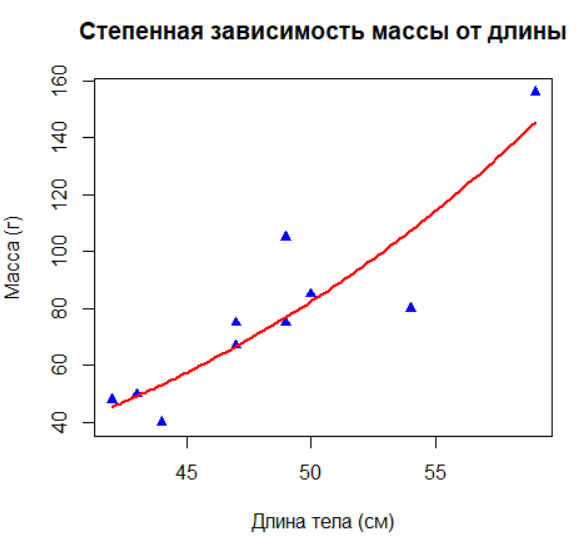
\includegraphics[width=0.6\linewidth,height=\textheight,keepaspectratio]{images/KOROSOV2.PNG}

}

\caption{Рис. 2.: Расчет степенной функции}

\end{figure}%

\section{ЛОГИСТИЧЕСКАЯ
РЕГРЕССИЯ}\label{ux43bux43eux433ux438ux441ux442ux438ux447ux435ux441ux43aux430ux44f-ux440ux435ux433ux440ux435ux441ux441ux438ux44f}

Вы изучите моделирование пороговых эффектов в экологии на примере
смертности дафний в зависимости от концентрации токсиканта. Построив
логистическую регрессию, вы получите S-образную кривую, характерную для
таких процессов.

\begin{Shaded}
\begin{Highlighting}[]
\CommentTok{\# Пример: смертность дафний при разных концентрациях токсиканта}
\CommentTok{\# Данные:}
\NormalTok{K }\OtherTok{\textless{}{-}} \FunctionTok{c}\NormalTok{(}\DecValTok{100}\NormalTok{, }\DecValTok{126}\NormalTok{, }\DecValTok{158}\NormalTok{, }\DecValTok{200}\NormalTok{, }\DecValTok{251}\NormalTok{, }\DecValTok{316}\NormalTok{, }\DecValTok{398}\NormalTok{, }\DecValTok{501}\NormalTok{, }\DecValTok{631}\NormalTok{, }\DecValTok{794}\NormalTok{, }\DecValTok{1000}\NormalTok{)}
\NormalTok{p }\OtherTok{\textless{}{-}} \FunctionTok{c}\NormalTok{(}\DecValTok{0}\NormalTok{, }\DecValTok{0}\NormalTok{, }\DecValTok{0}\NormalTok{, }\DecValTok{0}\NormalTok{, }\DecValTok{0}\NormalTok{, }\FloatTok{0.5}\NormalTok{, }\FloatTok{0.5}\NormalTok{, }\DecValTok{1}\NormalTok{, }\DecValTok{1}\NormalTok{, }\DecValTok{1}\NormalTok{, }\DecValTok{1}\NormalTok{)  }\CommentTok{\# Доля погибших}
\NormalTok{d }\OtherTok{\textless{}{-}} \FunctionTok{data.frame}\NormalTok{(K, p)}

\CommentTok{\# Построение логистической модели}
\NormalTok{logit\_model }\OtherTok{\textless{}{-}} \FunctionTok{glm}\NormalTok{(p }\SpecialCharTok{\textasciitilde{}}\NormalTok{ K, }\AttributeTok{family =} \FunctionTok{binomial}\NormalTok{(), }\AttributeTok{data =}\NormalTok{ d)}

\CommentTok{\# Визуализация S{-}образной кривой}
\FunctionTok{plot}\NormalTok{(d}\SpecialCharTok{$}\NormalTok{K, d}\SpecialCharTok{$}\NormalTok{p, }
     \AttributeTok{xlab =} \StringTok{"Концентрация токсиканта (мг/л)"}\NormalTok{, }
     \AttributeTok{ylab =} \StringTok{"Доля погибших"}\NormalTok{, }
     \AttributeTok{main =} \StringTok{"Токсическое воздействие на дафний"}\NormalTok{,}
     \AttributeTok{pch =} \DecValTok{19}\NormalTok{,}
     \AttributeTok{col =} \StringTok{"red"}\NormalTok{)}
\FunctionTok{lines}\NormalTok{(d}\SpecialCharTok{$}\NormalTok{K, }\FunctionTok{predict}\NormalTok{(logit\_model, }\AttributeTok{type =} \StringTok{"response"}\NormalTok{), }
      \AttributeTok{col =} \StringTok{"blue"}\NormalTok{, }\AttributeTok{lwd =} \DecValTok{2}\NormalTok{, }\AttributeTok{lty =} \DecValTok{1}\NormalTok{)}
\end{Highlighting}
\end{Shaded}

\begin{figure}[H]

{\centering 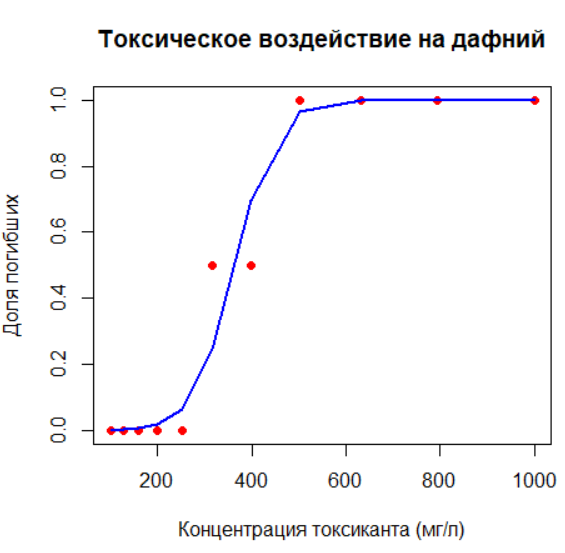
\includegraphics[width=0.6\linewidth,height=\textheight,keepaspectratio]{images/KOROSOV3.PNG}

}

\caption{Рис. 3.: Расчет логистической регрессии гибели дафний в
токсиканте}

\end{figure}%

\section{ПЕРЕХОД К
СЕТЯМ}\label{ux43fux435ux440ux435ux445ux43eux434-ux43a-ux441ux435ux442ux44fux43c}

Сделаем первый шаг к нейронным сетям, построив простейшую сеть без
скрытых слоев (аналог линейной регрессии) для модели токсичности. Вы
визуализируете структуру сети и убедитесь, что она дает результат,
аналогичный линейной модели.

\begin{Shaded}
\begin{Highlighting}[]
\CommentTok{\# Простейшая нейросеть (аналог линейной регрессии)}
\NormalTok{nn\_simple }\OtherTok{\textless{}{-}} \FunctionTok{neuralnet}\NormalTok{(p }\SpecialCharTok{\textasciitilde{}}\NormalTok{ K, }\AttributeTok{data =}\NormalTok{ d, }\AttributeTok{hidden =} \DecValTok{0}\NormalTok{)}

\CommentTok{\# Визуализация структуры сети}
\FunctionTok{plot}\NormalTok{(nn\_simple, }\AttributeTok{rep =} \StringTok{"best"}\NormalTok{)}
\end{Highlighting}
\end{Shaded}

\begin{figure}[H]

{\centering 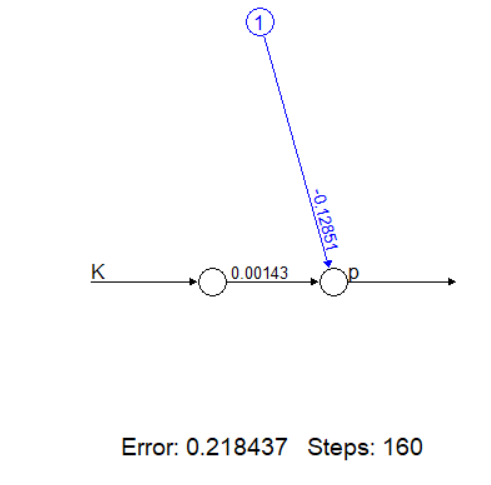
\includegraphics[width=0.4\linewidth,height=\textheight,keepaspectratio]{images/KOROSOV4.PNG}

}

\caption{Рис. 4.: Схема нейрона}

\end{figure}%

\section{НЕЙРОНЫ КАК НЕЛИНЕЙНЫЕ
ПРЕОБРАЗОВАТЕЛИ}\label{ux43dux435ux439ux440ux43eux43dux44b-ux43aux430ux43a-ux43dux435ux43bux438ux43dux435ux439ux43dux44bux435-ux43fux440ux435ux43eux431ux440ux430ux437ux43eux432ux430ux442ux435ux43bux438}

Здесь вы добавите в нейронную сеть скрытый слой с одним нейроном, что
позволит моделировать нелинейные зависимости. Вы сравните результат
работы такой сети с логистической регрессией и увидите, как нейронная
сеть имитирует пороговый эффект.

\begin{Shaded}
\begin{Highlighting}[]
\CommentTok{\# Сеть с одним скрытым нейроном (имитирует логистическую регрессию)}
\NormalTok{nn\_1hidden }\OtherTok{\textless{}{-}} \FunctionTok{neuralnet}\NormalTok{(p }\SpecialCharTok{\textasciitilde{}}\NormalTok{ K, }\AttributeTok{data =}\NormalTok{ d, }\AttributeTok{hidden =} \DecValTok{1}\NormalTok{)}

\CommentTok{\# Сравнение с логистической регрессией}
\FunctionTok{plot}\NormalTok{(d}\SpecialCharTok{$}\NormalTok{K, }\FunctionTok{predict}\NormalTok{(logit\_model, }\AttributeTok{type =} \StringTok{"response"}\NormalTok{), }
     \AttributeTok{type =} \StringTok{"l"}\NormalTok{, }
     \AttributeTok{col =} \StringTok{"darkgreen"}\NormalTok{, }
     \AttributeTok{lwd =} \DecValTok{2}\NormalTok{,}
     \AttributeTok{xlab =} \StringTok{"Концентрация"}\NormalTok{, }
     \AttributeTok{ylab =} \StringTok{"Смертность"}\NormalTok{,}
     \AttributeTok{main =} \StringTok{"Сравнение моделей"}\NormalTok{)}
\FunctionTok{lines}\NormalTok{(d}\SpecialCharTok{$}\NormalTok{K, }\FunctionTok{predict}\NormalTok{(nn\_1hidden, d), }\AttributeTok{col =} \StringTok{"blue"}\NormalTok{, }\AttributeTok{lty =} \DecValTok{2}\NormalTok{, }\AttributeTok{lwd =} \DecValTok{2}\NormalTok{)}
\FunctionTok{legend}\NormalTok{(}\StringTok{"bottomright"}\NormalTok{, }
       \AttributeTok{legend =} \FunctionTok{c}\NormalTok{(}\StringTok{"Логистическая регрессия"}\NormalTok{, }\StringTok{"Нейронная сеть (1 нейрон)"}\NormalTok{),}
       \AttributeTok{col =} \FunctionTok{c}\NormalTok{(}\StringTok{"darkgreen"}\NormalTok{, }\StringTok{"blue"}\NormalTok{), }
       \AttributeTok{lty =} \DecValTok{1}\SpecialCharTok{:}\DecValTok{2}\NormalTok{,}
       \AttributeTok{lwd =} \DecValTok{2}\NormalTok{)}
\end{Highlighting}
\end{Shaded}

\begin{figure}[H]

{\centering 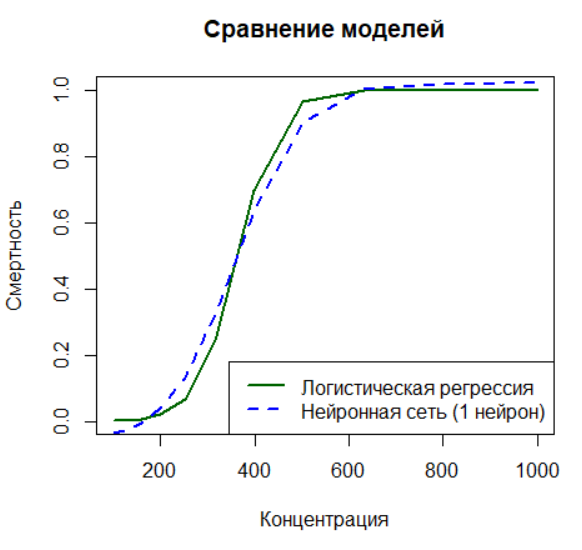
\includegraphics[width=0.4\linewidth,height=\textheight,keepaspectratio]{images/KOROSOV5.PNG}

}

\caption{Рис. 5.: Сравнение работы}

\end{figure}%

\section{КЛАССИФИКАЦИЯ В
ЭКОЛОГИИ}\label{ux43aux43bux430ux441ux441ux438ux444ux438ux43aux430ux446ux438ux44f-ux432-ux44dux43aux43eux43bux43eux433ux438ux438}

Вы примените нейронные сети для решения задачи классификации -
определения пола гадюк по морфометрическим признакам. Построив и сравнив
несколько архитектур сетей (без скрытых нейронов, с одним и тремя
нейронами), вы оцените их точность.

\begin{Shaded}
\begin{Highlighting}[]
\CommentTok{\# Загрузка данных по гадюкам (пол, длина тела, длина хвоста, масса)}
\NormalTok{v }\OtherTok{\textless{}{-}} \FunctionTok{read.csv}\NormalTok{(}\StringTok{"vipkar.csv"}\NormalTok{)}
\FunctionTok{head}\NormalTok{(v, }\DecValTok{3}\NormalTok{)  }\CommentTok{\# Просмотр первых строк данных}
\end{Highlighting}
\end{Shaded}

Модель без скрытых нейронов (аналог линейной регрессии)

\begin{Shaded}
\begin{Highlighting}[]
\NormalTok{nv0 }\OtherTok{\textless{}{-}} \FunctionTok{neuralnet}\NormalTok{(ns }\SpecialCharTok{\textasciitilde{}}\NormalTok{ lc, }\AttributeTok{data =}\NormalTok{ v, }\AttributeTok{hidden =} \DecValTok{0}\NormalTok{)}
\FunctionTok{plot}\NormalTok{(nv0)  }\CommentTok{\# Визуализация простейшей сети}
\end{Highlighting}
\end{Shaded}

\begin{figure}[H]

{\centering 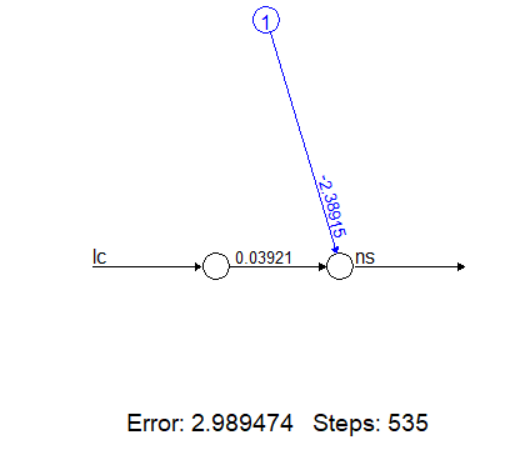
\includegraphics[width=0.4\linewidth,height=\textheight,keepaspectratio]{images/KOROSOV6.PNG}

}

\caption{Рис. 6.: Визуализация простейшей сети}

\end{figure}%

Модель с одним скрытым нейроном

\begin{Shaded}
\begin{Highlighting}[]
\NormalTok{nv1 }\OtherTok{\textless{}{-}} \FunctionTok{neuralnet}\NormalTok{(ns }\SpecialCharTok{\textasciitilde{}}\NormalTok{ lc, }\AttributeTok{data =}\NormalTok{ v, }\AttributeTok{hidden =} \DecValTok{1}\NormalTok{)}
\FunctionTok{plot}\NormalTok{(nv1)  }\CommentTok{\# Схема сети с одним нейроном}
\end{Highlighting}
\end{Shaded}

\begin{figure}[H]

{\centering 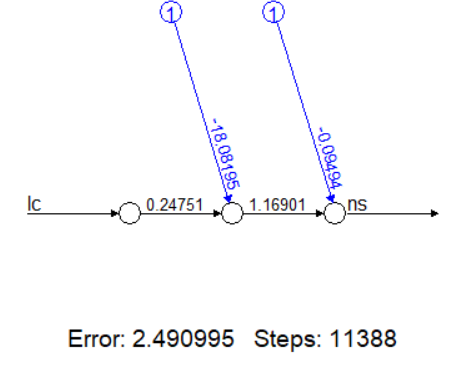
\includegraphics[width=0.4\linewidth,height=\textheight,keepaspectratio]{images/KOROSOV7.PNG}

}

\caption{Рис. 7.: Схема сети с одним нейроном}

\end{figure}%

Модель с тремя скрытыми нейронами (полноценная нейросеть)

\begin{Shaded}
\begin{Highlighting}[]
\NormalTok{nv3 }\OtherTok{\textless{}{-}} \FunctionTok{neuralnet}\NormalTok{(ns }\SpecialCharTok{\textasciitilde{}}\NormalTok{ lc }\SpecialCharTok{+}\NormalTok{ lt }\SpecialCharTok{+}\NormalTok{ w, }\AttributeTok{data =}\NormalTok{ v, }\AttributeTok{hidden =} \DecValTok{3}\NormalTok{)}
\FunctionTok{plot}\NormalTok{(nv3)  }\CommentTok{\# Визуализация сложной сети}
\end{Highlighting}
\end{Shaded}

\begin{figure}[H]

{\centering 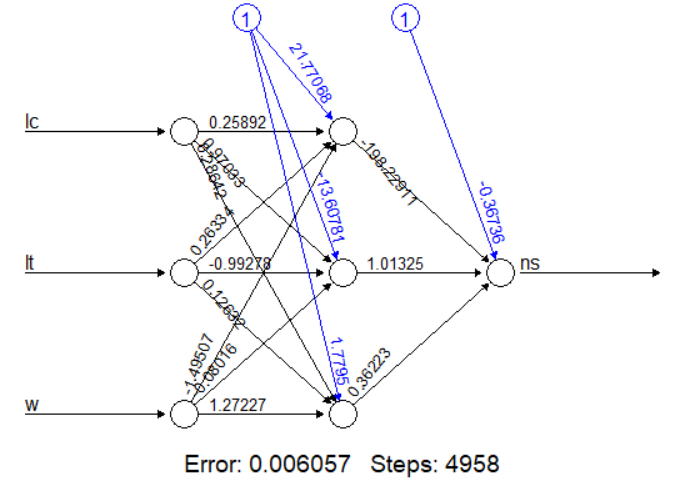
\includegraphics[width=0.4\linewidth,height=\textheight,keepaspectratio]{images/KOROSOV8.PNG}

}

\caption{Рис. 8.: Модель с тремя скрытыми нейронами}

\end{figure}%

Оценка точности классификации

\begin{Shaded}
\begin{Highlighting}[]
\NormalTok{predictions }\OtherTok{\textless{}{-}} \FunctionTok{predict}\NormalTok{(nv3, v)}
\NormalTok{predicted\_sex }\OtherTok{\textless{}{-}} \FunctionTok{round}\NormalTok{(predictions)}
\NormalTok{accuracy }\OtherTok{\textless{}{-}} \FunctionTok{mean}\NormalTok{(v}\SpecialCharTok{$}\NormalTok{ns }\SpecialCharTok{==}\NormalTok{ predicted\_sex)}
\FunctionTok{cat}\NormalTok{(}\StringTok{"Точность классификации:"}\NormalTok{, }\FunctionTok{round}\NormalTok{(accuracy}\SpecialCharTok{*}\DecValTok{100}\NormalTok{, }\DecValTok{1}\NormalTok{), }\StringTok{"\%}\SpecialCharTok{\textbackslash{}n}\StringTok{"}\NormalTok{)}
\end{Highlighting}
\end{Shaded}

Сравнение разных архитектур нейронных сетей (см. срипт
\href{https://mombus.github.io/cRab/data/KOROSOV_visual.R}{KOROSOV\_visual.R})

\begin{figure}[H]

{\centering 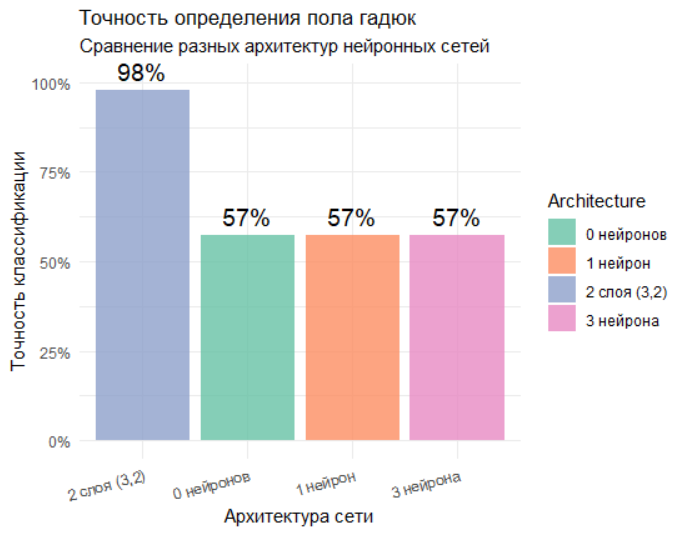
\includegraphics[width=0.6\linewidth,height=\textheight,keepaspectratio]{images/KOROSOV9.PNG}

}

\caption{Рис. 9.: Точность определения пола гадюк}

\end{figure}%

\section{ПРОСТРАНСТВЕННОЕ
МОДЕЛИРОВАНИЕ}\label{ux43fux440ux43eux441ux442ux440ux430ux43dux441ux442ux432ux435ux43dux43dux43eux435-ux43cux43eux434ux435ux43bux438ux440ux43eux432ux430ux43dux438ux435}

В завершение вы построите нейронную сеть для прогнозирования численности
гадюк на островах по характеристикам биотопов. Вы разделите данные на
обучающую и тестовую выборки, оцените точность модели и используете ее
для прогноза в новых условиях.

\begin{Shaded}
\begin{Highlighting}[]
\CommentTok{\# Данные по островам Кижского архипелага}
\NormalTok{v }\OtherTok{\textless{}{-}} \FunctionTok{read.csv}\NormalTok{(}\StringTok{"kihzsdat.csv"}\NormalTok{)}
\FunctionTok{head}\NormalTok{(v, }\DecValTok{3}\NormalTok{)  }\CommentTok{\# Структура данных: площадь, биотопы, численность видов}

\CommentTok{\# Случайное разделение данных на обучающую и тестовую выборки}
\FunctionTok{set.seed}\NormalTok{(}\DecValTok{123}\NormalTok{)  }\CommentTok{\# Для воспроизводимости}
\NormalTok{train\_indices }\OtherTok{\textless{}{-}} \FunctionTok{sample}\NormalTok{(}\DecValTok{1}\SpecialCharTok{:}\FunctionTok{nrow}\NormalTok{(v), }\DecValTok{12}\NormalTok{)}
\NormalTok{train\_data }\OtherTok{\textless{}{-}}\NormalTok{ v[train\_indices, ]}
\NormalTok{test\_data }\OtherTok{\textless{}{-}}\NormalTok{ v[}\SpecialCharTok{{-}}\NormalTok{train\_indices, ]}

\CommentTok{\# Построение нейросети с 5 нейронами в скрытом слое}
\NormalTok{model }\OtherTok{\textless{}{-}} \FunctionTok{neuralnet}\NormalTok{(vb }\SpecialCharTok{\textasciitilde{}}\NormalTok{ fo }\SpecialCharTok{+}\NormalTok{ me }\SpecialCharTok{+}\NormalTok{ bo, }\AttributeTok{data =}\NormalTok{ train\_data, }\AttributeTok{hidden =} \DecValTok{5}\NormalTok{)}

\CommentTok{\# Прогнозирование на обучающей выборке}
\NormalTok{train\_pred }\OtherTok{\textless{}{-}} \FunctionTok{predict}\NormalTok{(model, train\_data)}
\NormalTok{train\_accuracy }\OtherTok{\textless{}{-}} \FunctionTok{mean}\NormalTok{(}\FunctionTok{round}\NormalTok{(train\_pred) }\SpecialCharTok{==}\NormalTok{ train\_data}\SpecialCharTok{$}\NormalTok{vb)}
\FunctionTok{cat}\NormalTok{(}\StringTok{"Точность на обучающей выборке:"}\NormalTok{, }\FunctionTok{round}\NormalTok{(train\_accuracy}\SpecialCharTok{*}\DecValTok{100}\NormalTok{, }\DecValTok{1}\NormalTok{), }\StringTok{"\%}\SpecialCharTok{\textbackslash{}n}\StringTok{"}\NormalTok{)}

\CommentTok{\# Прогнозирование на тестовой выборке}
\NormalTok{test\_pred }\OtherTok{\textless{}{-}} \FunctionTok{predict}\NormalTok{(model, test\_data)}
\NormalTok{test\_accuracy }\OtherTok{\textless{}{-}} \FunctionTok{mean}\NormalTok{(}\FunctionTok{round}\NormalTok{(test\_pred) }\SpecialCharTok{==}\NormalTok{ test\_data}\SpecialCharTok{$}\NormalTok{vb)}
\FunctionTok{cat}\NormalTok{(}\StringTok{"Точность на тестовой выборке:"}\NormalTok{, }\FunctionTok{round}\NormalTok{(test\_accuracy}\SpecialCharTok{*}\DecValTok{100}\NormalTok{, }\DecValTok{1}\NormalTok{), }\StringTok{"\%}\SpecialCharTok{\textbackslash{}n}\StringTok{"}\NormalTok{)}

\CommentTok{\# Прогноз для новых условий (пример)}
\NormalTok{new\_conditions }\OtherTok{\textless{}{-}} \FunctionTok{data.frame}\NormalTok{(}
  \AttributeTok{fo =} \FunctionTok{c}\NormalTok{(}\FloatTok{57.9}\NormalTok{, }\FloatTok{35.3}\NormalTok{, }\FloatTok{83.0}\NormalTok{),  }\CommentTok{\# Площадь лесов (\%)}
  \AttributeTok{me =} \FunctionTok{c}\NormalTok{(}\FloatTok{4.1}\NormalTok{, }\FloatTok{0.0}\NormalTok{, }\FloatTok{7.3}\NormalTok{),     }\CommentTok{\# Площадь лугов (\%)}
  \AttributeTok{bo =} \FunctionTok{c}\NormalTok{(}\FloatTok{3.4}\NormalTok{, }\FloatTok{7.9}\NormalTok{, }\FloatTok{11.5}\NormalTok{)     }\CommentTok{\# Площадь болот (\%)}
\NormalTok{)}

\NormalTok{future\_pred }\OtherTok{\textless{}{-}} \FunctionTok{predict}\NormalTok{(model, new\_conditions)}
\FunctionTok{cat}\NormalTok{(}\StringTok{"Прогнозируемая численность гадюк:"}\NormalTok{, }\FunctionTok{round}\NormalTok{(future\_pred), }\StringTok{"}\SpecialCharTok{\textbackslash{}n}\StringTok{"}\NormalTok{)}
\end{Highlighting}
\end{Shaded}

\bookmarksetup{startatroot}

\chapter{Основы
картографии}\label{ux43eux441ux43dux43eux432ux44b-ux43aux430ux440ux442ux43eux433ux440ux430ux444ux438ux438}

\section{Введение}\label{ux432ux432ux435ux434ux435ux43dux438ux435-2}

Примеры карт и скрипты, которые могут быть полезны в рыбохозяйственных,
гидробиологическских и пр. океанологических исследованиях. На этом
занятии мы рассмотрим создание карт для визуализации пространственных
данных в исследованиях водных биоресурсов.

Вы научитесь создавать различные типы карт, используя современные пакеты
R, такие как \texttt{ggplot2}, \texttt{sf}, \texttt{rnaturalearth} и
другие. Мы начнем с простых карт распределения уловов по данным съемок,
затем перейдем к более сложным: картам с береговой линией, картам,
включающим нулевые уловы, распределению по квартилям. Далее рассмотрим
фасеточные карты для сравнения лет, карты с пространственной
автокорреляцией (LISA), а также промысловые карты (включая картограммы)
и гибридные карты, объединяющие данные съемок и промысла. В заключение
мы покажем, как создавать карты для раздела ``Материал и методы'' и
карты с врезками.

Обратите внимание, что примеры карт, представленные в интернете
(например, в HTML-версии этого документа), могут быть в уменьшенном
качестве. Однако при работе в R вы можете экспортировать полученные
графики в векторные (PDF, SVG) или растровые (PNG, TIFF) форматы с
высоким разрешением (до 600 dpi), что подходит для публикаций в научных
журналах.

\textbf{Для работы скрипта:}

\begin{enumerate}
\def\labelenumi{\arabic{enumi}.}
\item
  Скачайте файл данных
  (\href{https://mombus.github.io/cRab/data/KARTOGRAPHIC.xlsx}{KARTOGRAPHIC.xlsx})
\item
  Установите рабочую директорию в setwd()
\item
  Установите необходимые пакеты :
  \textbf{\texttt{install.packages(c("readxl",\ "tidyverse,\ "rnaturalearth",\ "sf",\ "viridis"\ ))}}
  \texttt{и\ др.}
\end{enumerate}

\section{Карта распределения уловов в
съемке}\label{ux43aux430ux440ux442ux430-ux440ux430ux441ux43fux440ux435ux434ux435ux43bux435ux43dux438ux44f-ux443ux43bux43eux432ux43eux432-ux432-ux441ux44aux435ux43cux43aux435}

Данная карта демонстрирует распределение уловов краба в ходе
исследовательской съемки. На ней отображены точки наблюдений, где размер
и цвет точек соответствуют величине улова.

\begin{figure}[H]

{\centering 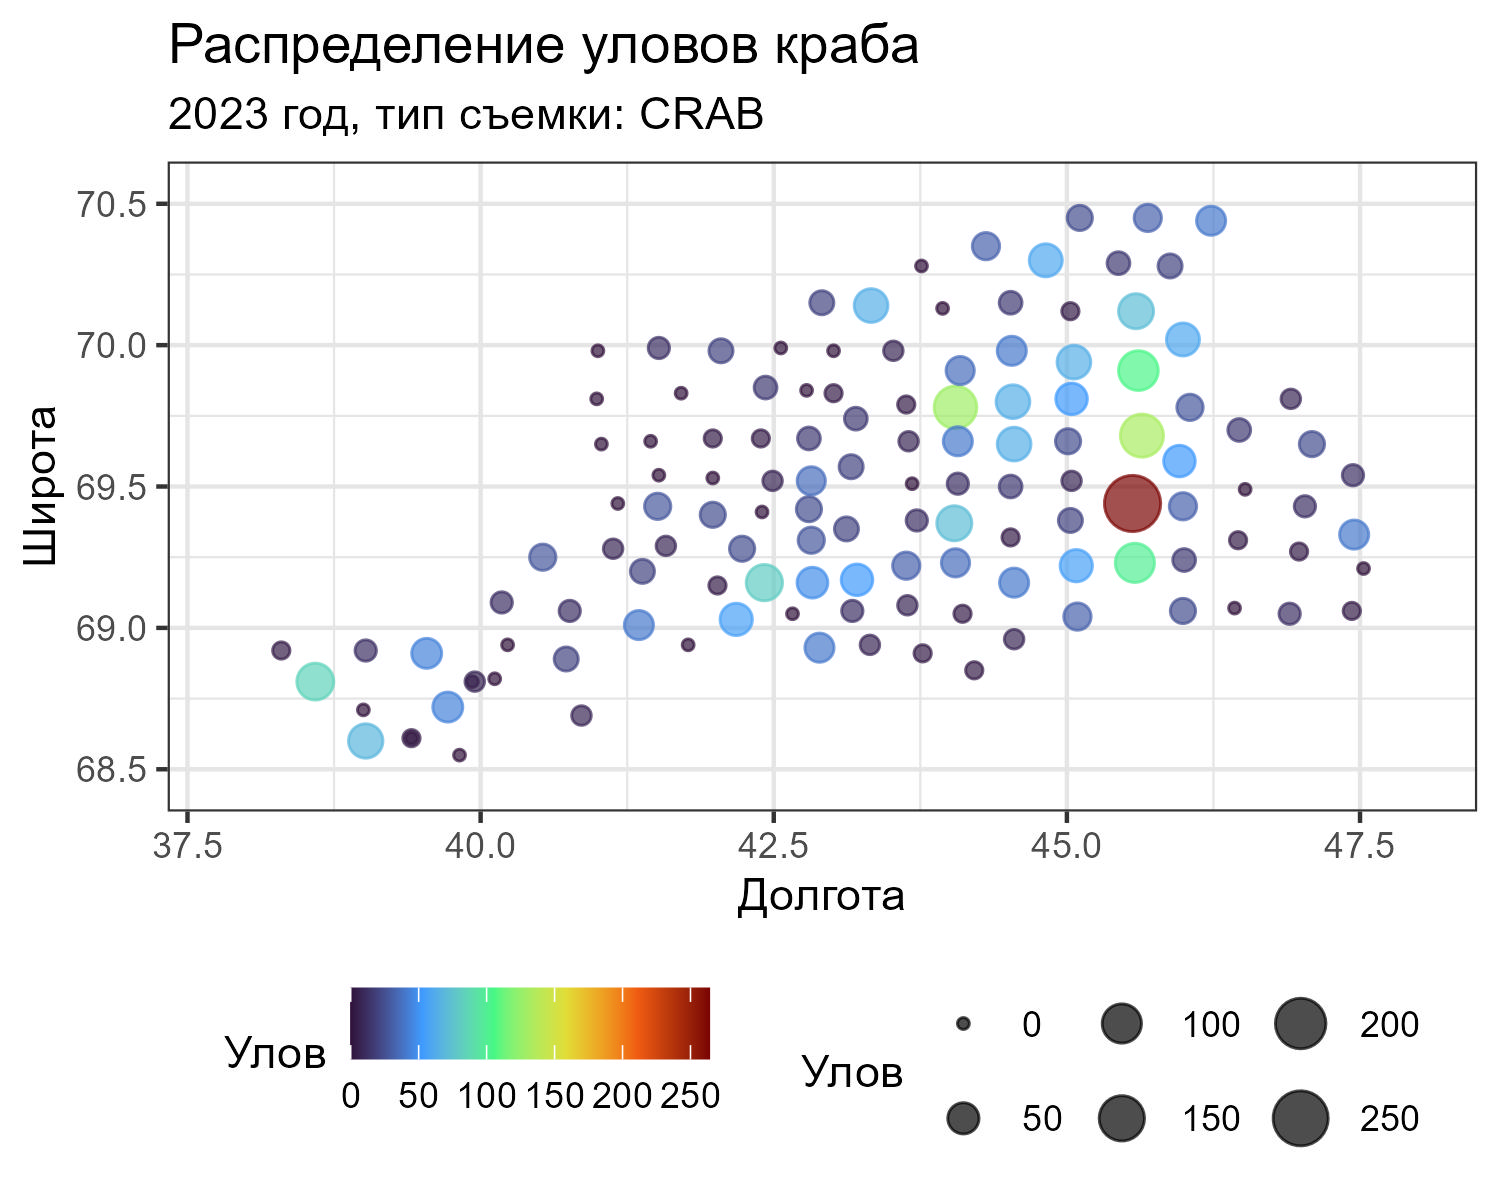
\includegraphics[width=0.7\linewidth,height=\textheight,keepaspectratio]{images/KARTOGRAPH1.PNG}

}

\caption{Рис. 1.: Пример карты распределения уловов в съемке}

\end{figure}%

В скрипте границы карты (лимиты) определяются автоматически с буфером,
но чаще их просто устанавливают вручную, например:

\begin{Shaded}
\begin{Highlighting}[]
\NormalTok{xmin }\OtherTok{\textless{}{-}} \DecValTok{37}
\NormalTok{xmax }\OtherTok{\textless{}{-}} \DecValTok{49}
\NormalTok{ymin }\OtherTok{\textless{}{-}} \FloatTok{68.5}
\NormalTok{ymax }\OtherTok{\textless{}{-}} \FloatTok{70.5}
\end{Highlighting}
\end{Shaded}

Скрипт карты целиком:

\begin{Shaded}
\begin{Highlighting}[]
\CommentTok{\# Очистка памяти и установка рабочей папки}
\FunctionTok{rm}\NormalTok{(}\AttributeTok{list =} \FunctionTok{ls}\NormalTok{())}
\FunctionTok{setwd}\NormalTok{(}\StringTok{"C:/COURSES/KARTOGRAPH/"}\NormalTok{)}

\CommentTok{\# Загрузка необходимых пакетов}
\FunctionTok{library}\NormalTok{(tidyverse)  }\CommentTok{\# Обработка данных и визуализация}
\FunctionTok{library}\NormalTok{(readxl)     }\CommentTok{\# Чтение Excel{-}файлов}

\CommentTok{\# 1. ЗАГРУЗКА ДАННЫХ}
\NormalTok{DATA }\OtherTok{\textless{}{-}} \FunctionTok{read\_excel}\NormalTok{(}\StringTok{"KARTOGRAPHIC.xlsx"}\NormalTok{, }\AttributeTok{sheet =} \StringTok{"SURVEY"}\NormalTok{) }\SpecialCharTok{\%\textgreater{}\%} 
  \FunctionTok{filter}\NormalTok{(YEAR }\SpecialCharTok{==} \DecValTok{2023}\NormalTok{, SURV }\SpecialCharTok{==} \StringTok{"CRAB"}\NormalTok{)  }\CommentTok{\# Фильтр для 2023 года и съемки CRAB}

\CommentTok{\# 2. АВТОМАТИЧЕСКИЙ РАСЧЕТ ГРАНИЦ С БУФЕРОМ 5\%}
\CommentTok{\# Расчет диапазонов координат}
\NormalTok{x\_range }\OtherTok{\textless{}{-}} \FunctionTok{range}\NormalTok{(DATA}\SpecialCharTok{$}\NormalTok{X, }\AttributeTok{na.rm =} \ConstantTok{TRUE}\NormalTok{)}
\NormalTok{y\_range }\OtherTok{\textless{}{-}} \FunctionTok{range}\NormalTok{(DATA}\SpecialCharTok{$}\NormalTok{Y, }\AttributeTok{na.rm =} \ConstantTok{TRUE}\NormalTok{)}

\CommentTok{\# Расчет 5\% буфера}
\NormalTok{x\_buffer }\OtherTok{\textless{}{-}} \FloatTok{0.05} \SpecialCharTok{*} \FunctionTok{diff}\NormalTok{(x\_range)}
\NormalTok{y\_buffer }\OtherTok{\textless{}{-}} \FloatTok{0.05} \SpecialCharTok{*} \FunctionTok{diff}\NormalTok{(y\_range)}

\CommentTok{\# Установка границ с буфером}
\NormalTok{xmin }\OtherTok{\textless{}{-}}\NormalTok{ x\_range[}\DecValTok{1}\NormalTok{] }\SpecialCharTok{{-}}\NormalTok{ x\_buffer}
\NormalTok{xmax }\OtherTok{\textless{}{-}}\NormalTok{ x\_range[}\DecValTok{2}\NormalTok{] }\SpecialCharTok{+}\NormalTok{ x\_buffer}
\NormalTok{ymin }\OtherTok{\textless{}{-}}\NormalTok{ y\_range[}\DecValTok{1}\NormalTok{] }\SpecialCharTok{{-}}\NormalTok{ y\_buffer}
\NormalTok{ymax }\OtherTok{\textless{}{-}}\NormalTok{ y\_range[}\DecValTok{2}\NormalTok{] }\SpecialCharTok{+}\NormalTok{ y\_buffer}

\CommentTok{\# 3. ВИЗУАЛИЗАЦИЯ ТОЧЕК}
\FunctionTok{ggplot}\NormalTok{(DATA) }\SpecialCharTok{+}
  \CommentTok{\# Точки наблюдений с размером и цветом по величине улова}
  \FunctionTok{geom\_point}\NormalTok{(}\FunctionTok{aes}\NormalTok{(}\AttributeTok{x =}\NormalTok{ X, }\AttributeTok{y =}\NormalTok{ Y, }\AttributeTok{size =}\NormalTok{ PROM, }\AttributeTok{color =}\NormalTok{ PROM), }\AttributeTok{alpha =} \FloatTok{0.7}\NormalTok{) }\SpecialCharTok{+}
  
  \CommentTok{\# Цветовая шкала (виридисная палитра)}
  \FunctionTok{scale\_color\_viridis\_c}\NormalTok{(}\AttributeTok{option =} \StringTok{"H"}\NormalTok{, }\AttributeTok{name =} \StringTok{"Улов"}\NormalTok{) }\SpecialCharTok{+}
  
  \CommentTok{\# Шкала размеров точек}
  \FunctionTok{scale\_size\_continuous}\NormalTok{(}\AttributeTok{name =} \StringTok{"Улов"}\NormalTok{) }\SpecialCharTok{+}
  
  \CommentTok{\# Настройка границ с автоматически рассчитанными значениями}
  \FunctionTok{coord\_cartesian}\NormalTok{(}\AttributeTok{xlim =} \FunctionTok{c}\NormalTok{(xmin, xmax), }\AttributeTok{ylim =} \FunctionTok{c}\NormalTok{(ymin, ymax)) }\SpecialCharTok{+}
  
  \CommentTok{\# Подписи осей}
  \FunctionTok{labs}\NormalTok{(}\AttributeTok{x =} \StringTok{"Долгота"}\NormalTok{, }\AttributeTok{y =} \StringTok{"Широта"}\NormalTok{, }
       \AttributeTok{title =} \StringTok{"Распределение уловов краба"}\NormalTok{, }
       \AttributeTok{subtitle =} \StringTok{"2023 год, тип съемки: CRAB"}\NormalTok{) }\SpecialCharTok{+}
  
  \CommentTok{\# Оформление графика}
  \FunctionTok{theme\_bw}\NormalTok{() }\SpecialCharTok{+}
  \FunctionTok{theme}\NormalTok{(}
    \AttributeTok{panel.grid =} \FunctionTok{element\_line}\NormalTok{(}\AttributeTok{color =} \StringTok{"grey90"}\NormalTok{),}
    \AttributeTok{legend.position =} \StringTok{"bottom"}
\NormalTok{  )}
\end{Highlighting}
\end{Shaded}

\section{Карта распределения уловов в съемке с береговой
линией}\label{ux43aux430ux440ux442ux430-ux440ux430ux441ux43fux440ux435ux434ux435ux43bux435ux43dux438ux44f-ux443ux43bux43eux432ux43eux432-ux432-ux441ux44aux435ux43cux43aux435-ux441-ux431ux435ux440ux435ux433ux43eux432ux43eux439-ux43bux438ux43dux438ux435ux439}

\begin{figure}[H]

{\centering 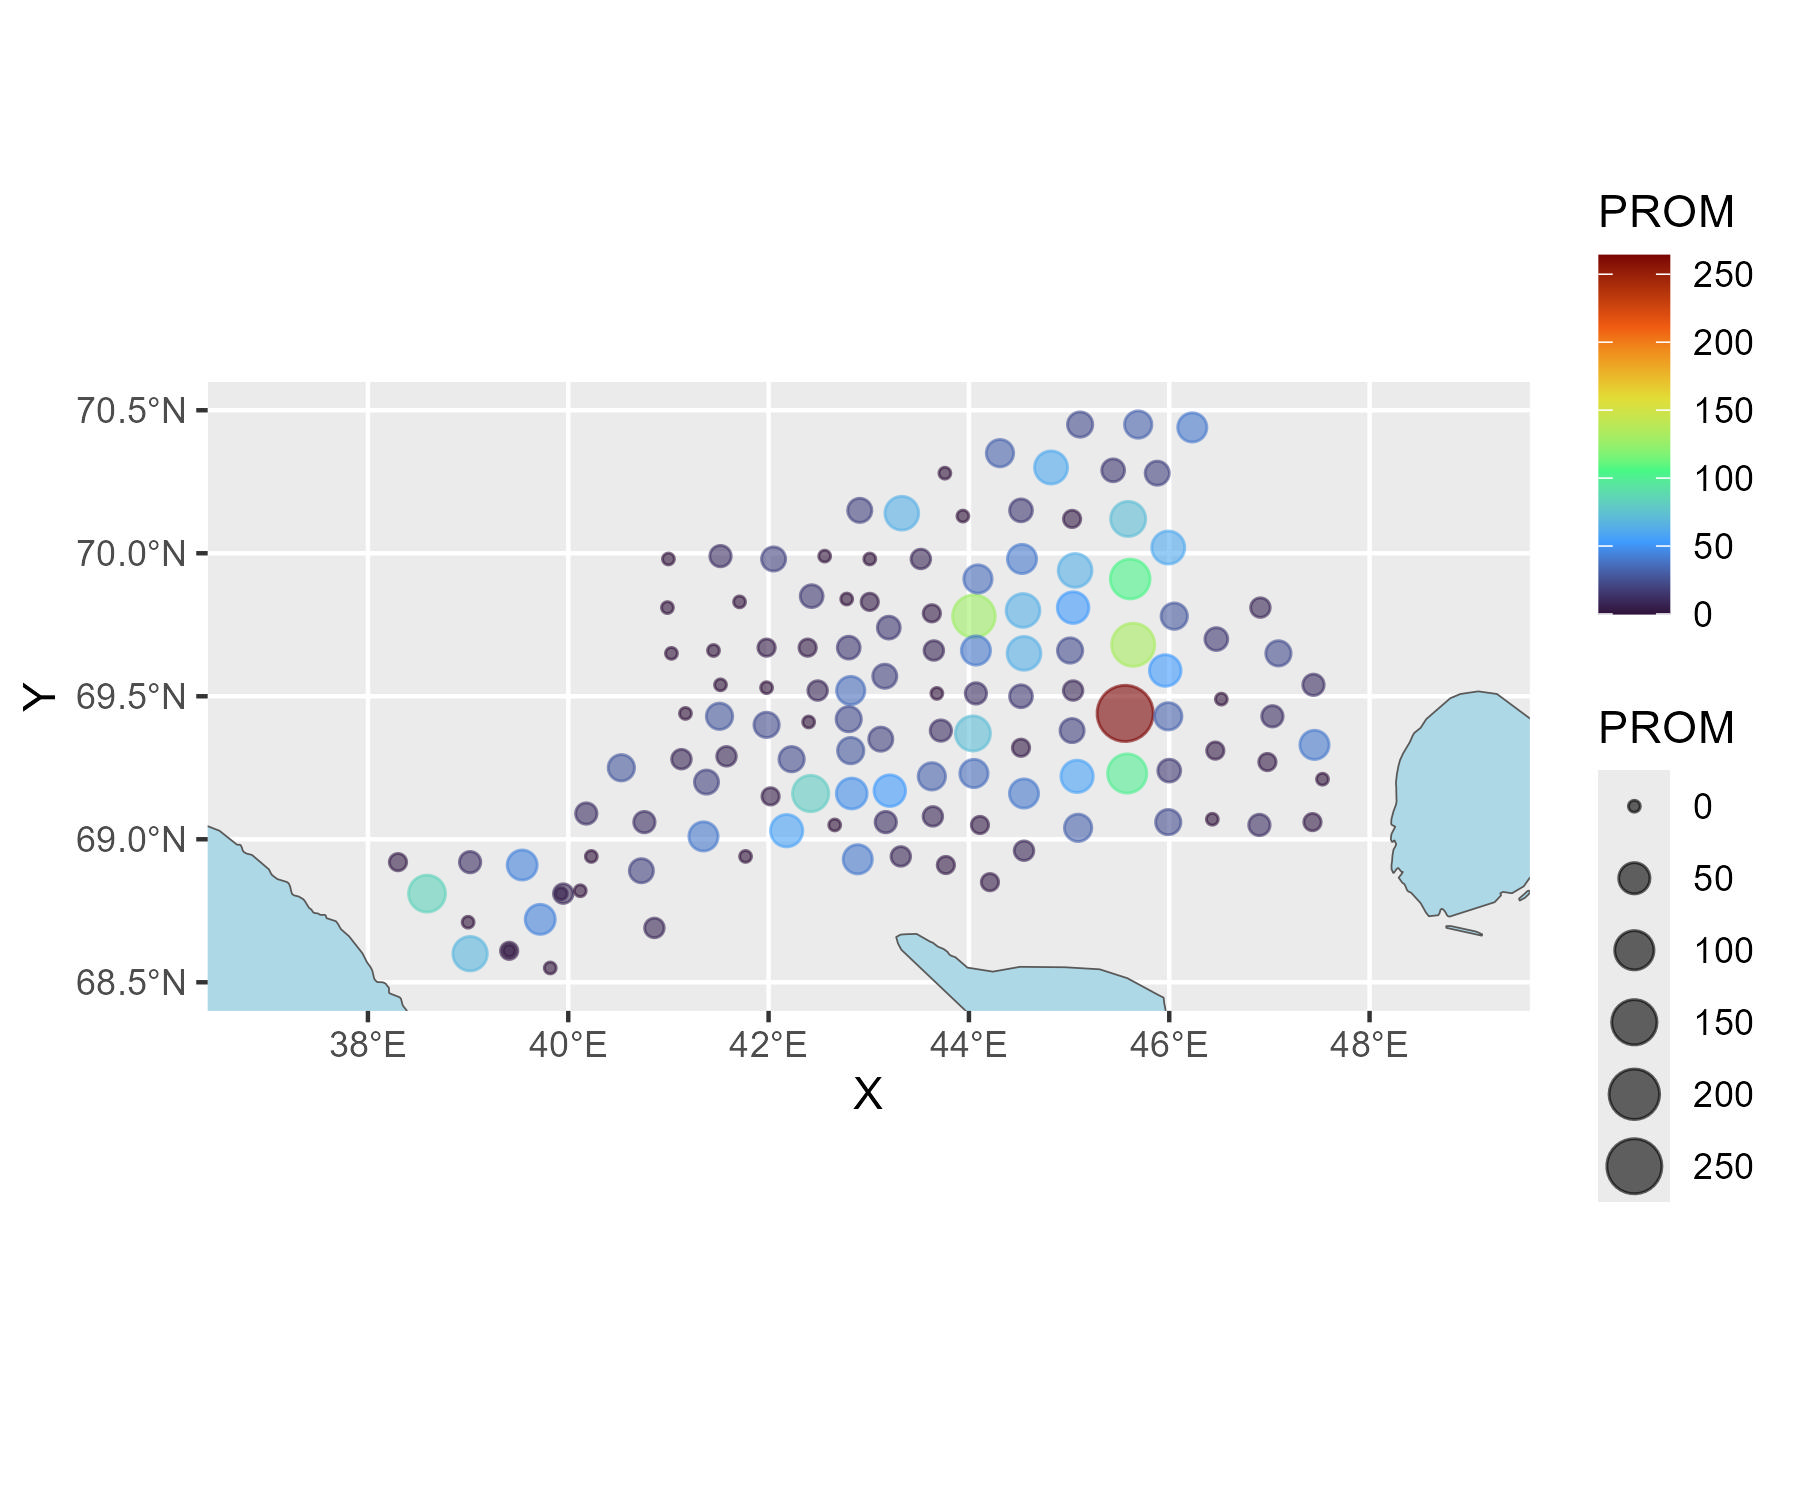
\includegraphics[width=0.7\linewidth,height=\textheight,keepaspectratio]{images/KARTOGRAPH2.PNG}

}

\caption{Рис. 2.: Пример карты распределения уловов в съемке с береговой
линией}

\end{figure}%

\begin{Shaded}
\begin{Highlighting}[]
\CommentTok{\# Очистка окружения и установка рабочей директории}
\FunctionTok{rm}\NormalTok{(}\AttributeTok{list =} \FunctionTok{ls}\NormalTok{())  }\CommentTok{\# Удаление всех объектов из глобального окружения}
\FunctionTok{setwd}\NormalTok{(}\StringTok{"C:/COURSES/KARTOGRAPH/"}\NormalTok{)  }\CommentTok{\# Установка рабочей директории}

\CommentTok{\# Загрузка необходимых библиотек}
\FunctionTok{library}\NormalTok{(rnaturalearth)  }\CommentTok{\# Для получения векторных карт мира}
\FunctionTok{library}\NormalTok{(tidyverse)      }\CommentTok{\# Коллекция пакетов для работы с данными}
\FunctionTok{library}\NormalTok{(sf)             }\CommentTok{\# Пространственный анализ}

\DocumentationTok{\#\#\#\#\#\#\# ЗАГРУЗКА ДАННЫХ И ПОДГОТОВКА ПРОСТРАНСТВЕННЫХ ОБЪЕКТОВ \#\#\#\#\#\#\#\#\#\#\#\#\#\#\#\#}

\CommentTok{\# Чтение и фильтрация данных}
\NormalTok{DATA }\OtherTok{\textless{}{-}}\NormalTok{ readxl}\SpecialCharTok{::}\FunctionTok{read\_excel}\NormalTok{(}\StringTok{"KARTOGRAPHIC.xlsx"}\NormalTok{, }\AttributeTok{sheet =} \StringTok{"SURVEY"}\NormalTok{) }\SpecialCharTok{\%\textgreater{}\%} 
  \FunctionTok{filter}\NormalTok{(YEAR }\SpecialCharTok{==} \DecValTok{2023}\NormalTok{, SURV }\SpecialCharTok{==} \StringTok{"CRAB"}\NormalTok{)  }\CommentTok{\# Фильтр данных за 2023 год по типу съемки}

\CommentTok{\# Получение границ России}
\NormalTok{russia }\OtherTok{\textless{}{-}} \FunctionTok{ne\_countries}\NormalTok{(}\AttributeTok{scale =} \DecValTok{10}\NormalTok{, }\AttributeTok{country =} \StringTok{"Russia"}\NormalTok{)  }\CommentTok{\# Загрузка векторных границ (масштаб 1:10м)}

\CommentTok{\# Установка границ отображаемой области (долгота/широта)}
\NormalTok{xmin}\OtherTok{=}\DecValTok{37}  \CommentTok{\# Западная граница}
\NormalTok{xmax}\OtherTok{=}\DecValTok{49}  \CommentTok{\# Восточная граница}
\NormalTok{ymin}\OtherTok{=}\FloatTok{68.5} \CommentTok{\# Южная граница}
\NormalTok{ymax}\OtherTok{=}\FloatTok{70.5} \CommentTok{\# Северная граница}

\CommentTok{\# Построение карты}
\FunctionTok{ggplot}\NormalTok{() }\SpecialCharTok{+}
  \CommentTok{\# Базовая карта России}
  \FunctionTok{geom\_sf}\NormalTok{(}\AttributeTok{data =}\NormalTok{ russia, }\AttributeTok{fill =} \StringTok{"lightblue"}\NormalTok{) }\SpecialCharTok{+} 
  \CommentTok{\# Ограничение области отображения}
  \FunctionTok{coord\_sf}\NormalTok{(}\AttributeTok{xlim =} \FunctionTok{c}\NormalTok{(xmin, xmax), }\AttributeTok{ylim =} \FunctionTok{c}\NormalTok{(ymin, ymax)) }\SpecialCharTok{+}
  \CommentTok{\# Точки наблюдений с размером и цветом по переменной PROM}
  \FunctionTok{geom\_point}\NormalTok{(}\FunctionTok{aes}\NormalTok{(}\AttributeTok{x =}\NormalTok{ X, }\AttributeTok{y =}\NormalTok{ Y, }\AttributeTok{size =}\NormalTok{ PROM, }\AttributeTok{color =}\NormalTok{ PROM),}
             \AttributeTok{data =}\NormalTok{ DATA, }\AttributeTok{alpha =} \FloatTok{0.6}\NormalTok{) }\SpecialCharTok{+}
  \CommentTok{\# Цветовая шкала (viridis, вариант H)}
  \FunctionTok{scale\_color\_viridis\_c}\NormalTok{(}\AttributeTok{option =} \StringTok{"H"}\NormalTok{)}
\end{Highlighting}
\end{Shaded}

\section{Карта распределения уловов, включая
нулевые}\label{ux43aux430ux440ux442ux430-ux440ux430ux441ux43fux440ux435ux434ux435ux43bux435ux43dux438ux44f-ux443ux43bux43eux432ux43eux432-ux432ux43aux43bux44eux447ux430ux44f-ux43dux443ux43bux435ux432ux44bux435}

\begin{figure}[H]

{\centering 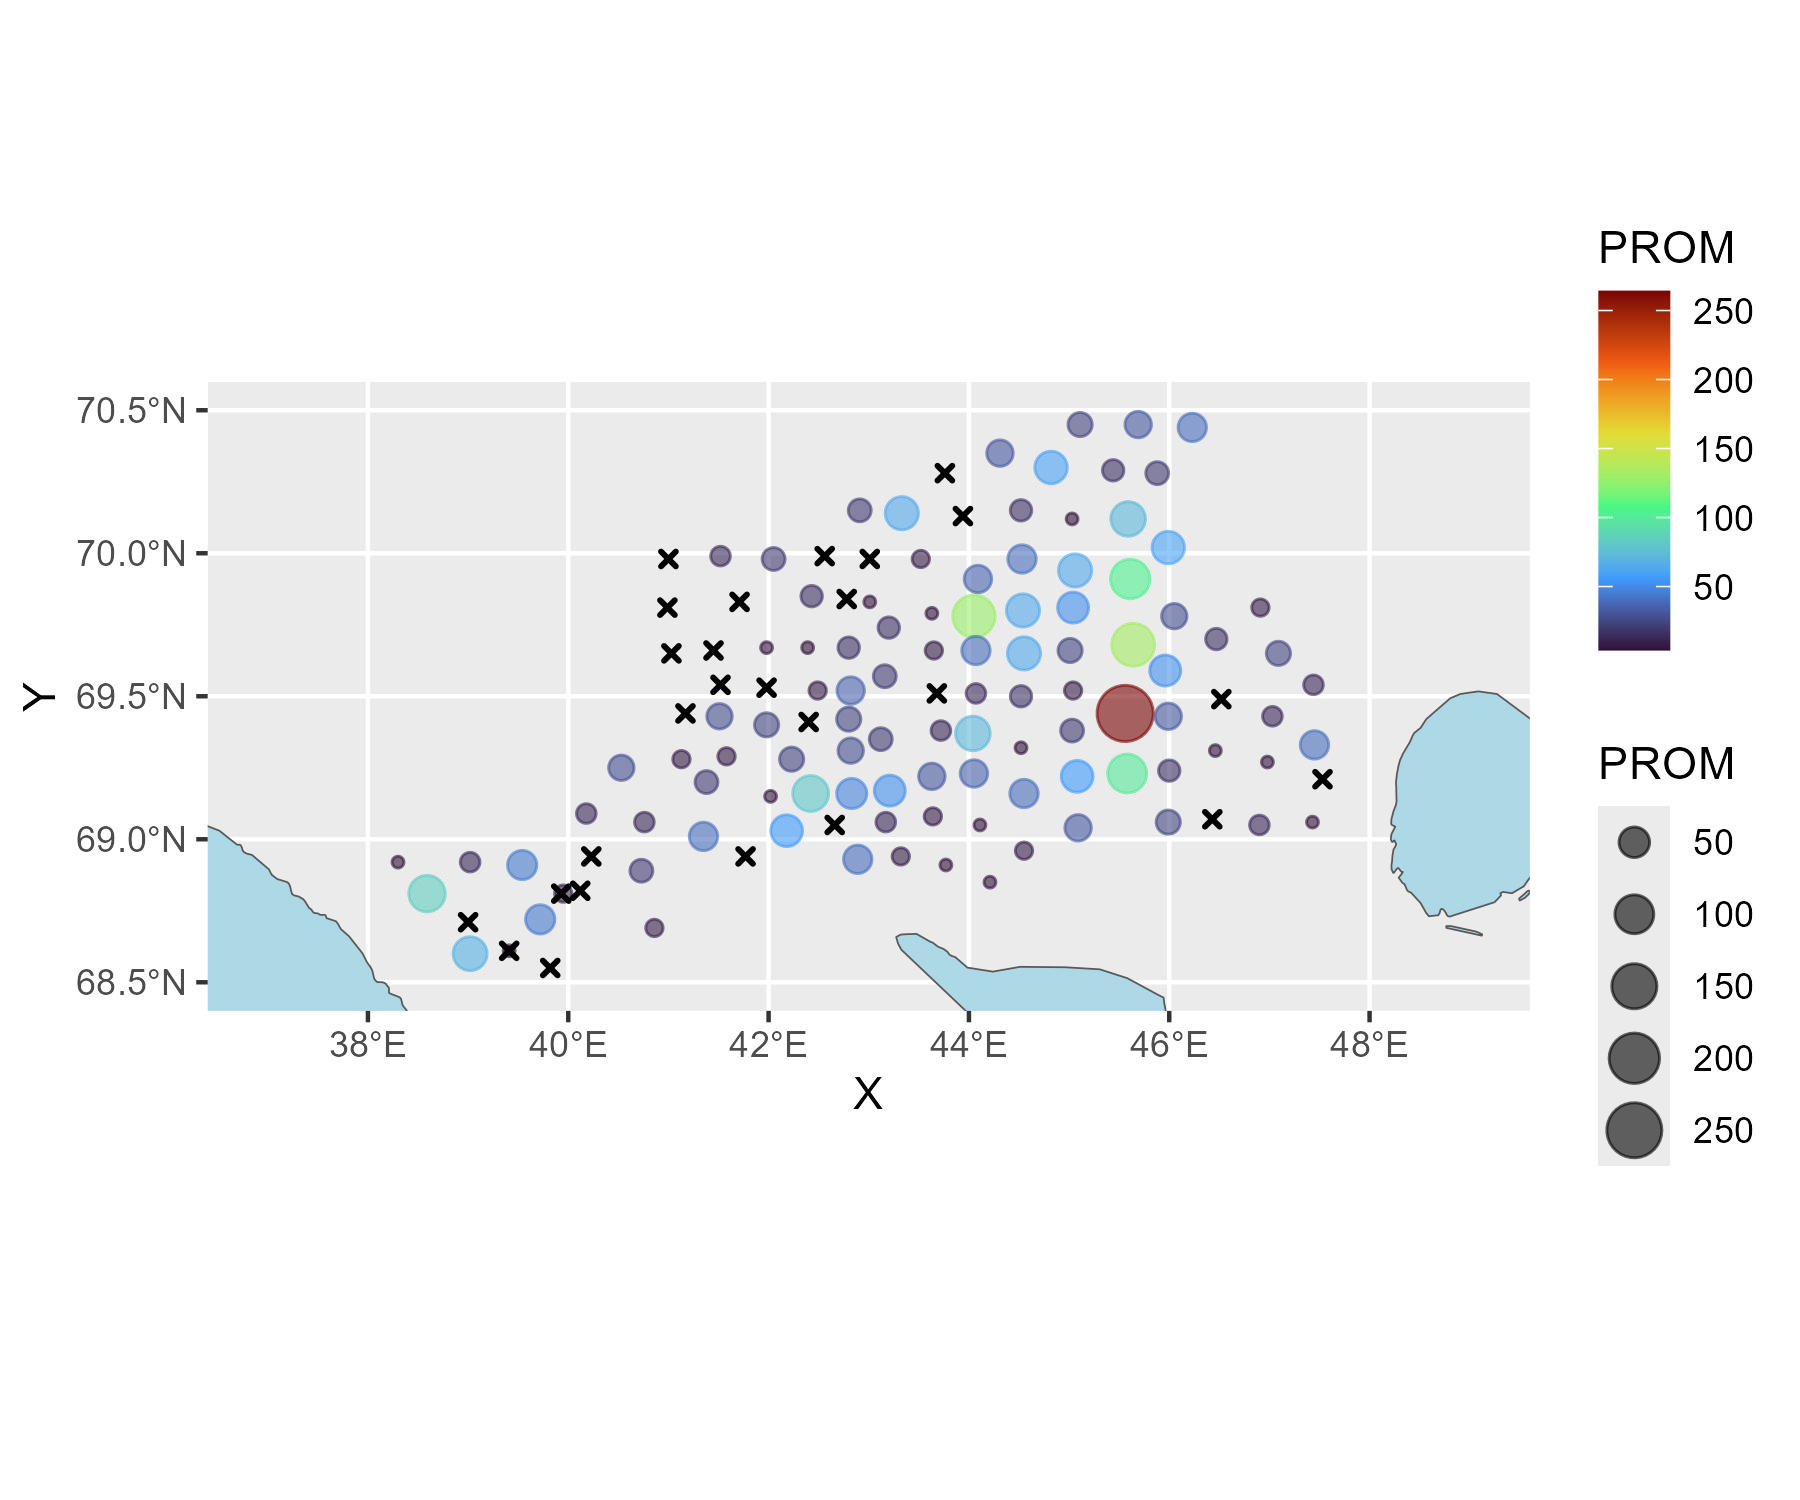
\includegraphics[width=0.7\linewidth,height=\textheight,keepaspectratio]{images/KARTOGRAPH3.PNG}

}

\caption{Рис. 3.: Карта распределения уловов, включая нулевые}

\end{figure}%

\begin{Shaded}
\begin{Highlighting}[]
\CommentTok{\# Очистка окружения и установка рабочей директории}
\FunctionTok{rm}\NormalTok{(}\AttributeTok{list =} \FunctionTok{ls}\NormalTok{())  }\CommentTok{\# Удаление всех объектов из глобального окружения}
\FunctionTok{setwd}\NormalTok{(}\StringTok{"C:/COURSES/KARTOGRAPH/"}\NormalTok{)  }\CommentTok{\# Установка рабочей директории}

\CommentTok{\# Загрузка необходимых библиотек}
\FunctionTok{library}\NormalTok{(rnaturalearth)  }\CommentTok{\# Для получения векторных карт мира}
\FunctionTok{library}\NormalTok{(tidyverse)      }\CommentTok{\# Коллекция пакетов для работы с данными}
\FunctionTok{library}\NormalTok{(sf)             }\CommentTok{\# Пространственный анализ}

\DocumentationTok{\#\#\#\#\#\#\# ЗАГРУЗКА ДАННЫХ И ПОДГОТОВКА ПРОСТРАНСТВЕННЫХ ОБЪЕКТОВ \#\#\#\#\#\#\#\#\#\#\#\#\#\#\#\#}

\CommentTok{\# Чтение и фильтрация данных}
\NormalTok{DATA }\OtherTok{\textless{}{-}}\NormalTok{ readxl}\SpecialCharTok{::}\FunctionTok{read\_excel}\NormalTok{(}\StringTok{"KARTOGRAPHIC.xlsx"}\NormalTok{, }\AttributeTok{sheet =} \StringTok{"SURVEY"}\NormalTok{) }\SpecialCharTok{\%\textgreater{}\%} 
  \FunctionTok{filter}\NormalTok{(YEAR }\SpecialCharTok{==} \DecValTok{2023}\NormalTok{, SURV }\SpecialCharTok{==} \StringTok{"CRAB"}\NormalTok{)  }\CommentTok{\# Фильтр данных за 2023 год по типу съемки}

\CommentTok{\# Получение границ России}
\NormalTok{russia }\OtherTok{\textless{}{-}} \FunctionTok{ne\_countries}\NormalTok{(}\AttributeTok{scale =} \DecValTok{10}\NormalTok{, }\AttributeTok{country =} \StringTok{"Russia"}\NormalTok{)  }\CommentTok{\# Загрузка векторных границ (масштаб 1:10м)}

\CommentTok{\# Установка границ отображаемой области (долгота/широта)}
\NormalTok{xmin}\OtherTok{=}\DecValTok{37}  \CommentTok{\# Западная граница}
\NormalTok{xmax}\OtherTok{=}\DecValTok{49}  \CommentTok{\# Восточная граница}
\NormalTok{ymin}\OtherTok{=}\FloatTok{68.5} \CommentTok{\# Южная граница}
\NormalTok{ymax}\OtherTok{=}\FloatTok{70.5} \CommentTok{\# Северная граница}

\CommentTok{\# Построение карты}
\FunctionTok{ggplot}\NormalTok{() }\SpecialCharTok{+}
  \CommentTok{\# Базовая карта России}
  \FunctionTok{geom\_sf}\NormalTok{(}\AttributeTok{data =}\NormalTok{ russia, }\AttributeTok{fill =} \StringTok{"lightblue"}\NormalTok{) }\SpecialCharTok{+} 
  \CommentTok{\# Ограничение области отображения}
  \FunctionTok{coord\_sf}\NormalTok{(}\AttributeTok{xlim =} \FunctionTok{c}\NormalTok{(xmin, xmax), }\AttributeTok{ylim =} \FunctionTok{c}\NormalTok{(ymin, ymax)) }\SpecialCharTok{+}
  \CommentTok{\# Точки наблюдений с размером и цветом по переменной PROM (ненулевые уловы)}
  \FunctionTok{geom\_point}\NormalTok{(}\FunctionTok{aes}\NormalTok{(}\AttributeTok{x =}\NormalTok{ X, }\AttributeTok{y =}\NormalTok{ Y, }\AttributeTok{size =}\NormalTok{ PROM, }\AttributeTok{color =}\NormalTok{ PROM),}
             \AttributeTok{data =} \FunctionTok{filter}\NormalTok{(DATA, PROM }\SpecialCharTok{\textgreater{}} \DecValTok{0}\NormalTok{), }\AttributeTok{alpha =} \FloatTok{0.6}\NormalTok{) }\SpecialCharTok{+}
  \CommentTok{\# Точки для нулевых уловов (крестики)}
  \FunctionTok{geom\_point}\NormalTok{(}\FunctionTok{aes}\NormalTok{(}\AttributeTok{x =}\NormalTok{ X, }\AttributeTok{y =}\NormalTok{ Y),}
             \AttributeTok{data =} \FunctionTok{filter}\NormalTok{(DATA, PROM }\SpecialCharTok{==} \DecValTok{0}\NormalTok{),}
             \AttributeTok{shape =} \DecValTok{4}\NormalTok{, }\AttributeTok{size =} \DecValTok{1}\NormalTok{, }\AttributeTok{stroke =} \DecValTok{1}\NormalTok{, }\AttributeTok{color =} \StringTok{"black"}\NormalTok{) }\SpecialCharTok{+}
  \CommentTok{\# Цветовая шкала (viridis, вариант H)}
  \FunctionTok{scale\_color\_viridis\_c}\NormalTok{(}\AttributeTok{option =} \StringTok{"H"}\NormalTok{)}
\end{Highlighting}
\end{Shaded}

\section{Карта распределения уловов, распределенных по
квартилям}\label{ux43aux430ux440ux442ux430-ux440ux430ux441ux43fux440ux435ux434ux435ux43bux435ux43dux438ux44f-ux443ux43bux43eux432ux43eux432-ux440ux430ux441ux43fux440ux435ux434ux435ux43bux435ux43dux43dux44bux445-ux43fux43e-ux43aux432ux430ux440ux442ux438ux43bux44fux43c}

\begin{figure}[H]

{\centering 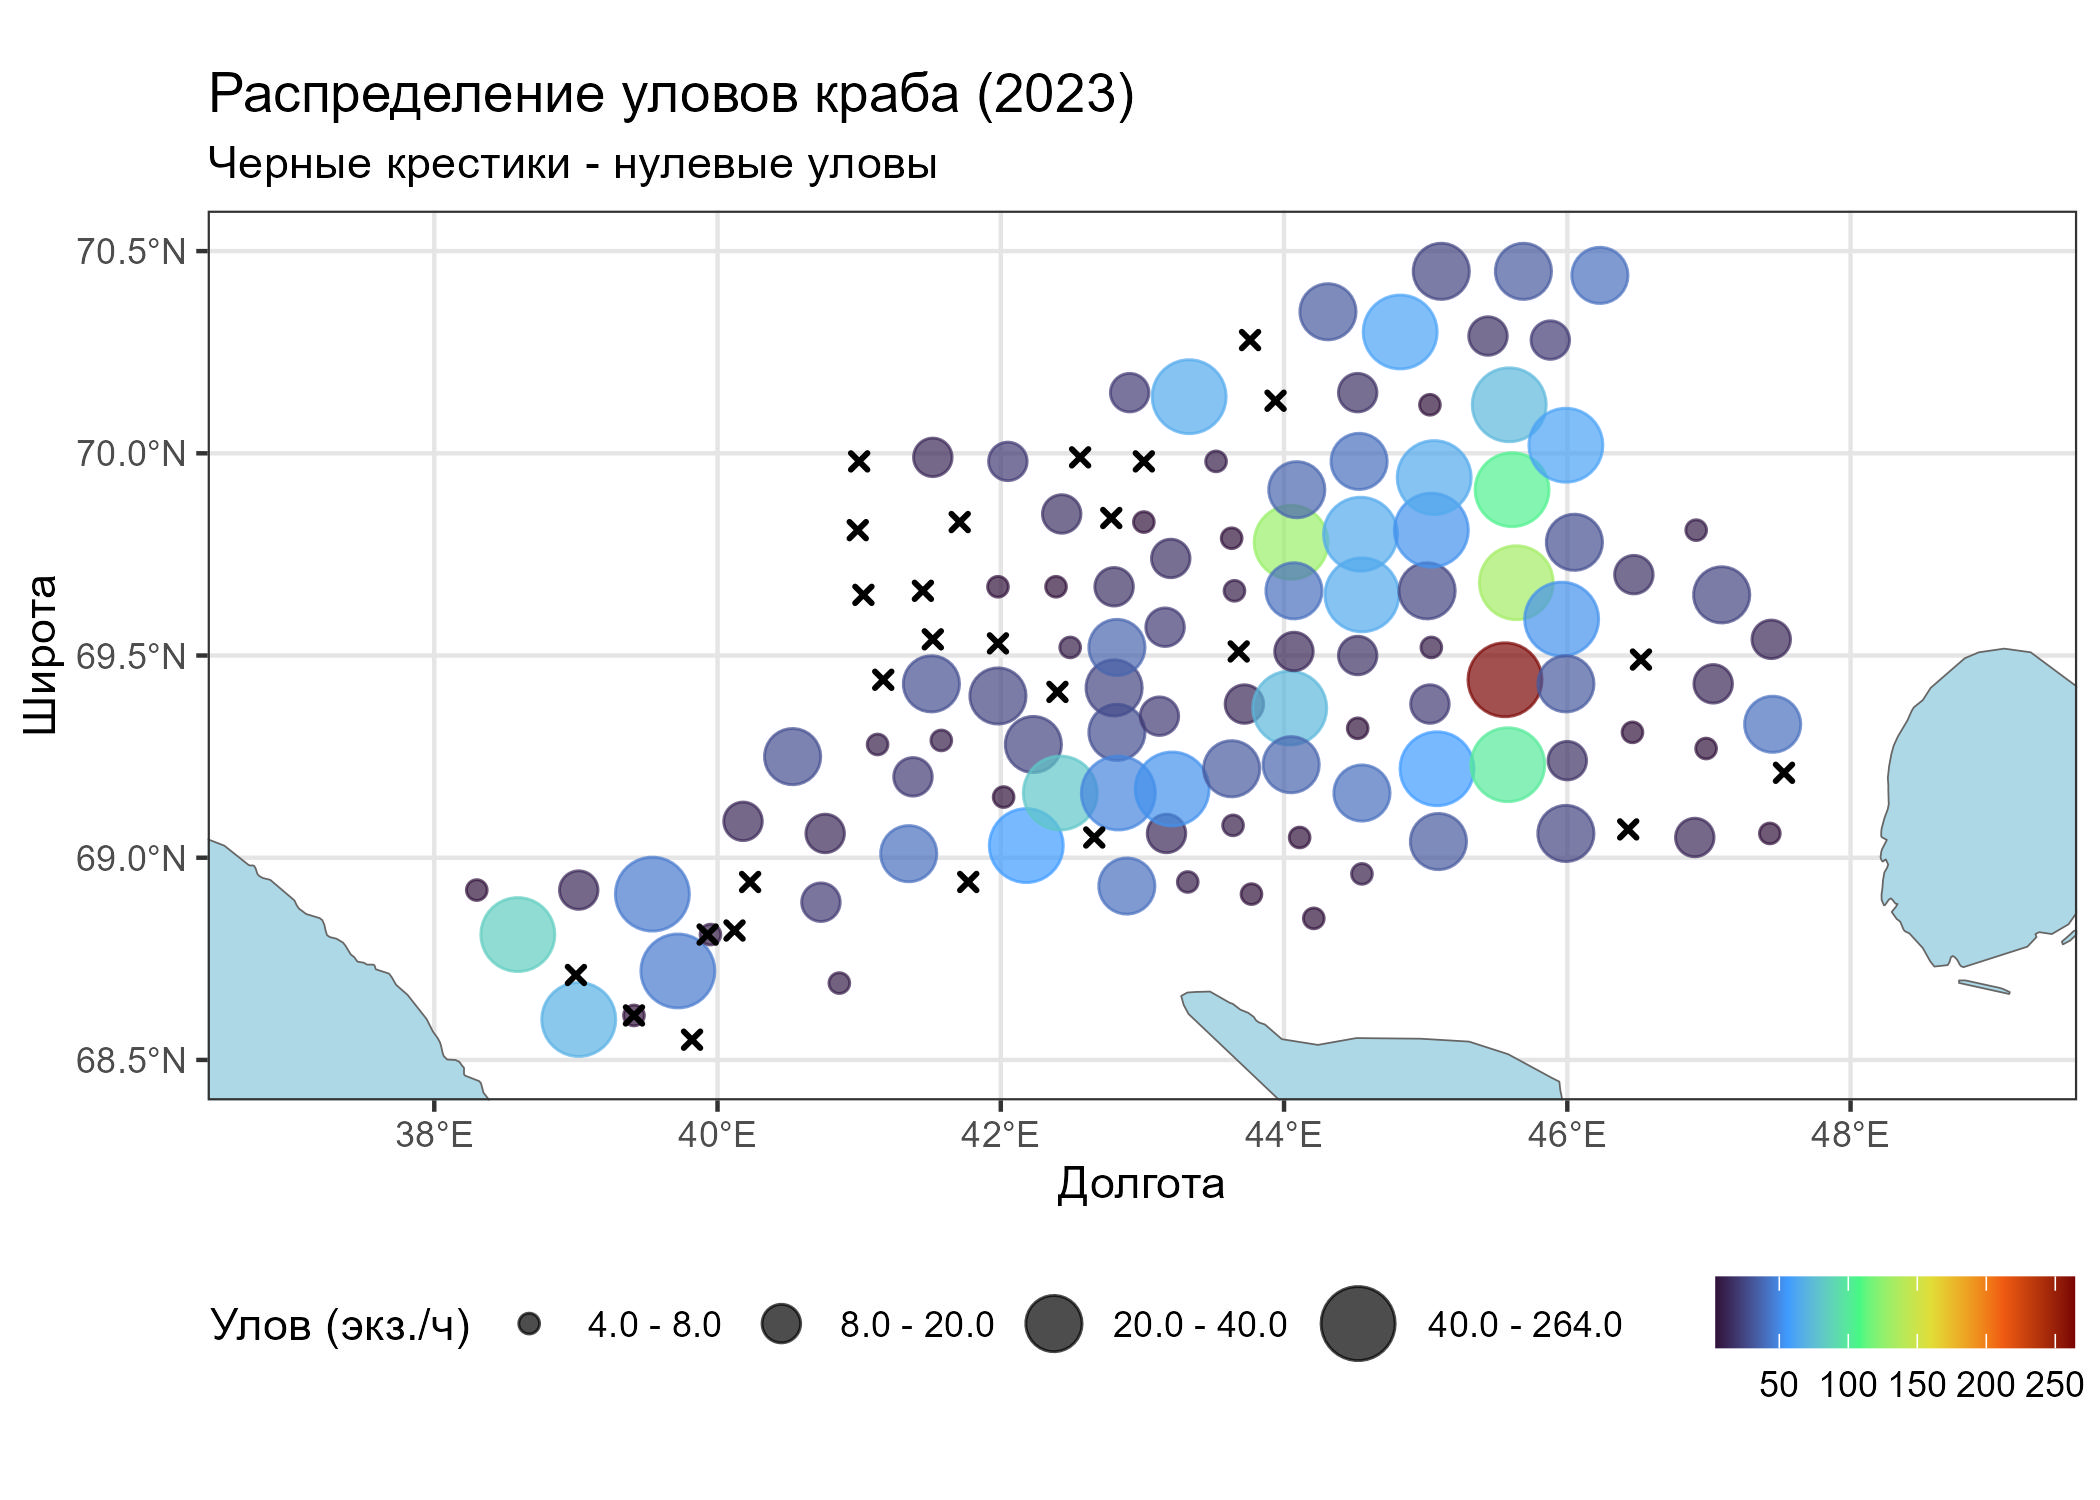
\includegraphics[width=0.7\linewidth,height=\textheight,keepaspectratio]{images/KARTOGRAPH4.PNG}

}

\caption{Рис. 4.: Карта распределения уловов, распределенных по
квартилям}

\end{figure}%

\begin{Shaded}
\begin{Highlighting}[]
\CommentTok{\# Очистка окружения и установка рабочей директории}
\FunctionTok{rm}\NormalTok{(}\AttributeTok{list =} \FunctionTok{ls}\NormalTok{())}
\FunctionTok{setwd}\NormalTok{(}\StringTok{"C:/COURSES/KARTOGRAPH/"}\NormalTok{)}

\CommentTok{\# Загрузка необходимых библиотек}
\FunctionTok{library}\NormalTok{(rnaturalearth)}
\FunctionTok{library}\NormalTok{(tidyverse)}
\FunctionTok{library}\NormalTok{(sf)}

\DocumentationTok{\#\#\#\#\#\#\# ЗАГРУЗКА ДАННЫХ И ПОДГОТОВКА ПРОСТРАНСТВЕННЫХ ОБЪЕКТОВ \#\#\#\#\#\#\#\#\#\#\#\#\#\#\#\#}

\CommentTok{\# Чтение и фильтрация данных}
\NormalTok{DATA }\OtherTok{\textless{}{-}}\NormalTok{ readxl}\SpecialCharTok{::}\FunctionTok{read\_excel}\NormalTok{(}\StringTok{"KARTOGRAPHIC.xlsx"}\NormalTok{, }\AttributeTok{sheet =} \StringTok{"SURVEY"}\NormalTok{) }\SpecialCharTok{\%\textgreater{}\%} 
  \FunctionTok{filter}\NormalTok{(YEAR }\SpecialCharTok{==} \DecValTok{2023}\NormalTok{, SURV }\SpecialCharTok{==} \StringTok{"CRAB"}\NormalTok{)}

\CommentTok{\# Получение границ России}
\NormalTok{russia }\OtherTok{\textless{}{-}} \FunctionTok{ne\_countries}\NormalTok{(}\AttributeTok{scale =} \DecValTok{10}\NormalTok{, }\AttributeTok{country =} \StringTok{"Russia"}\NormalTok{) }\SpecialCharTok{\%\textgreater{}\%} 
  \FunctionTok{st\_as\_sf}\NormalTok{()}

\CommentTok{\# Установка границ отображаемой области}
\NormalTok{xmin}\OtherTok{=}\DecValTok{37}\NormalTok{; xmax}\OtherTok{=}\DecValTok{49}\NormalTok{; ymin}\OtherTok{=}\FloatTok{68.5}\NormalTok{; ymax}\OtherTok{=}\FloatTok{70.5}

\DocumentationTok{\#\#\#\#\#\#\# ПОДГОТОВКА ДАННЫХ ДЛЯ ВИЗУАЛИЗАЦИИ \#\#\#\#\#\#\#\#\#\#\#\#\#\#\#\#}
\CommentTok{\# Вычисляем квартили отдельно}
\NormalTok{quantiles }\OtherTok{\textless{}{-}} \FunctionTok{quantile}\NormalTok{(DATA}\SpecialCharTok{$}\NormalTok{PROM[DATA}\SpecialCharTok{$}\NormalTok{PROM }\SpecialCharTok{\textgreater{}} \DecValTok{0}\NormalTok{], }\AttributeTok{probs =} \FunctionTok{seq}\NormalTok{(}\DecValTok{0}\NormalTok{, }\DecValTok{1}\NormalTok{, }\FloatTok{0.25}\NormalTok{))}

\CommentTok{\# Создаем 4 категории с реальными диапазонами значений}
\NormalTok{nonzero\_data }\OtherTok{\textless{}{-}}\NormalTok{ DATA }\SpecialCharTok{\%\textgreater{}\%} 
  \FunctionTok{filter}\NormalTok{(PROM }\SpecialCharTok{\textgreater{}} \DecValTok{0}\NormalTok{) }\SpecialCharTok{\%\textgreater{}\%}
  \FunctionTok{mutate}\NormalTok{(}
    \AttributeTok{PROM\_cat =} \FunctionTok{cut}\NormalTok{(}
\NormalTok{      PROM,}
      \AttributeTok{breaks =}\NormalTok{ quantiles,}
      \AttributeTok{include.lowest =} \ConstantTok{TRUE}\NormalTok{,}
      \AttributeTok{labels =} \FunctionTok{c}\NormalTok{(}
        \FunctionTok{sprintf}\NormalTok{(}\StringTok{"\%.1f {-} \%.1f"}\NormalTok{, quantiles[}\DecValTok{1}\NormalTok{], quantiles[}\DecValTok{2}\NormalTok{]),}
        \FunctionTok{sprintf}\NormalTok{(}\StringTok{"\%.1f {-} \%.1f"}\NormalTok{, quantiles[}\DecValTok{2}\NormalTok{], quantiles[}\DecValTok{3}\NormalTok{]),}
        \FunctionTok{sprintf}\NormalTok{(}\StringTok{"\%.1f {-} \%.1f"}\NormalTok{, quantiles[}\DecValTok{3}\NormalTok{], quantiles[}\DecValTok{4}\NormalTok{]),}
        \FunctionTok{sprintf}\NormalTok{(}\StringTok{"\%.1f {-} \%.1f"}\NormalTok{, quantiles[}\DecValTok{4}\NormalTok{], quantiles[}\DecValTok{5}\NormalTok{])}
\NormalTok{      )}
\NormalTok{    )}
\NormalTok{  )}

\CommentTok{\# Построение карты}
\FunctionTok{ggplot}\NormalTok{() }\SpecialCharTok{+}
  \CommentTok{\# Базовая карта России}
  \FunctionTok{geom\_sf}\NormalTok{(}\AttributeTok{data =}\NormalTok{ russia, }\AttributeTok{fill =} \StringTok{"lightblue"}\NormalTok{, }\AttributeTok{color =} \StringTok{"gray40"}\NormalTok{) }\SpecialCharTok{+} 
  \CommentTok{\# Ограничение области отображения}
  \FunctionTok{coord\_sf}\NormalTok{(}\AttributeTok{xlim =} \FunctionTok{c}\NormalTok{(xmin, xmax), }\AttributeTok{ylim =} \FunctionTok{c}\NormalTok{(ymin, ymax)) }\SpecialCharTok{+}
  \CommentTok{\# Точки наблюдений с категориальным размером}
  \FunctionTok{geom\_point}\NormalTok{(}
    \AttributeTok{data =}\NormalTok{ nonzero\_data,}
    \FunctionTok{aes}\NormalTok{(}\AttributeTok{x =}\NormalTok{ X, }\AttributeTok{y =}\NormalTok{ Y, }\AttributeTok{size =}\NormalTok{ PROM\_cat, }\AttributeTok{color =}\NormalTok{ PROM),}
    \AttributeTok{alpha =} \FloatTok{0.7}
\NormalTok{  ) }\SpecialCharTok{+}
  \CommentTok{\# Точки для нулевых уловов (крестики)}
  \FunctionTok{geom\_point}\NormalTok{(}
    \AttributeTok{data =} \FunctionTok{filter}\NormalTok{(DATA, PROM }\SpecialCharTok{==} \DecValTok{0}\NormalTok{),}
    \FunctionTok{aes}\NormalTok{(}\AttributeTok{x =}\NormalTok{ X, }\AttributeTok{y =}\NormalTok{ Y),}
    \AttributeTok{shape =} \DecValTok{4}\NormalTok{, }\AttributeTok{size =} \FloatTok{1.2}\NormalTok{, }\AttributeTok{stroke =} \DecValTok{1}\NormalTok{, }\AttributeTok{color =} \StringTok{"black"}
\NormalTok{  ) }\SpecialCharTok{+}
  \CommentTok{\# Цветовая шкала (непрерывная)}
  \FunctionTok{scale\_color\_viridis\_c}\NormalTok{(}\AttributeTok{option =} \StringTok{"H"}\NormalTok{, }\AttributeTok{name =} \ConstantTok{NULL}\NormalTok{) }\SpecialCharTok{+}
  \CommentTok{\# Ручная настройка размеров для категорий}
  \FunctionTok{scale\_size\_manual}\NormalTok{(}
    \AttributeTok{name =} \StringTok{"Улов (экз./ч)"}\NormalTok{,}
    \AttributeTok{values =} \FunctionTok{c}\NormalTok{(}\DecValTok{2}\NormalTok{, }\DecValTok{4}\NormalTok{, }\DecValTok{6}\NormalTok{, }\DecValTok{8}\NormalTok{),  }\CommentTok{\# Размеры точек для категорий}
    \AttributeTok{drop =} \ConstantTok{FALSE}
\NormalTok{  ) }\SpecialCharTok{+}
  \CommentTok{\# Настройки темы}
  \FunctionTok{theme\_bw}\NormalTok{() }\SpecialCharTok{+}
  \FunctionTok{labs}\NormalTok{(}
    \AttributeTok{title =} \StringTok{"Распределение уловов краба (2023)"}\NormalTok{,}
    \AttributeTok{subtitle =} \StringTok{"Черные крестики {-} нулевые уловы"}\NormalTok{,}
    \AttributeTok{x =} \StringTok{"Долгота"}\NormalTok{, }
    \AttributeTok{y =} \StringTok{"Широта"}
\NormalTok{  ) }\SpecialCharTok{+}
  \FunctionTok{theme}\NormalTok{(}
    \AttributeTok{panel.grid =} \FunctionTok{element\_line}\NormalTok{(}\AttributeTok{color =} \StringTok{"gray90"}\NormalTok{),}
    \AttributeTok{legend.position =} \StringTok{"bottom"}
\NormalTok{  )}
\end{Highlighting}
\end{Shaded}

\section{Карта распределения уловов по
фасеткам}\label{ux43aux430ux440ux442ux430-ux440ux430ux441ux43fux440ux435ux434ux435ux43bux435ux43dux438ux44f-ux443ux43bux43eux432ux43eux432-ux43fux43e-ux444ux430ux441ux435ux442ux43aux430ux43c}

\begin{figure}[H]

{\centering 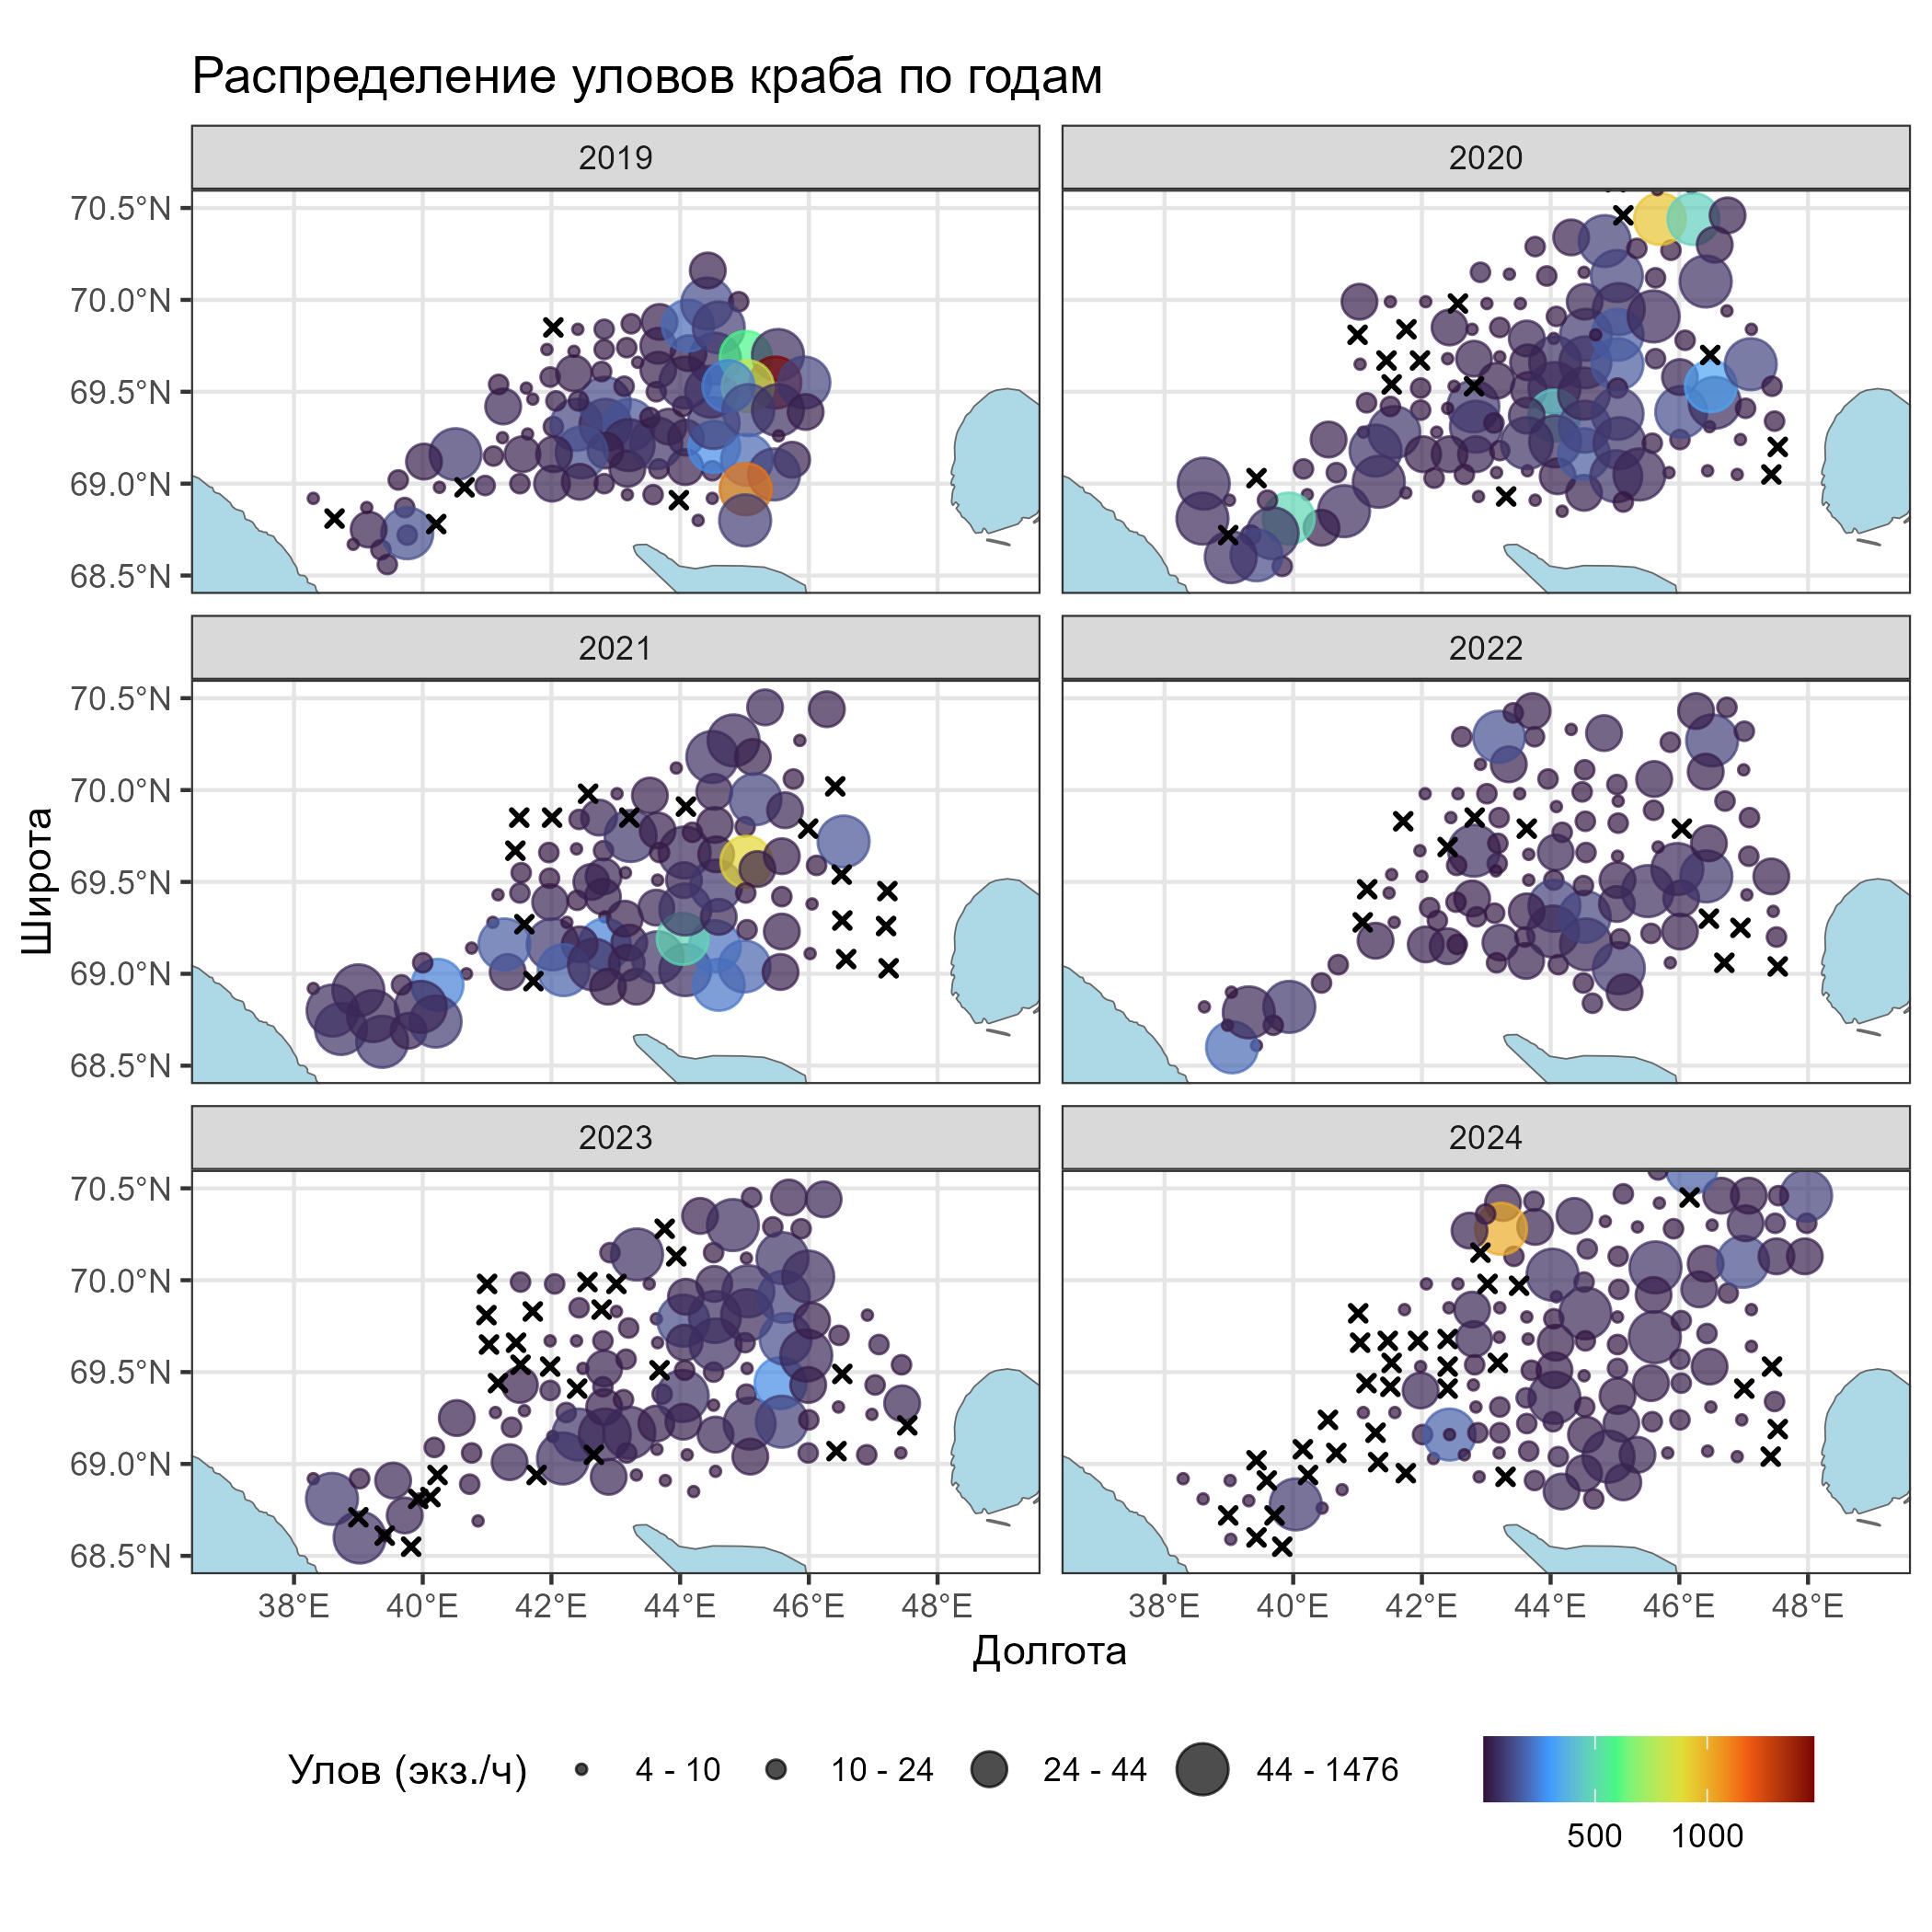
\includegraphics[width=0.8\linewidth,height=\textheight,keepaspectratio]{images/KARTOGRAPH5.PNG}

}

\caption{Рис. 5.: Карта распределения уловов по фасеткам}

\end{figure}%

\begin{Shaded}
\begin{Highlighting}[]
\CommentTok{\# Очистка окружения и установка рабочей директории}
\FunctionTok{rm}\NormalTok{(}\AttributeTok{list =} \FunctionTok{ls}\NormalTok{())}
\FunctionTok{setwd}\NormalTok{(}\StringTok{"C:/COURSES/KARTOGRAPH/"}\NormalTok{)}

\CommentTok{\# Установка и подключение библиотек (если не установлено — раскомментируй)}
\CommentTok{\# install.packages(c("rnaturalearth", "tidyverse", "sf", "readxl", "viridis"))}
\FunctionTok{library}\NormalTok{(rnaturalearth)}
\FunctionTok{library}\NormalTok{(tidyverse)}
\FunctionTok{library}\NormalTok{(sf)}
\FunctionTok{library}\NormalTok{(readxl)}
\FunctionTok{library}\NormalTok{(viridis)}

\DocumentationTok{\#\#\#\#\#\#\# ЗАГРУЗКА ДАННЫХ И ПОДГОТОВКА ПРОСТРАНСТВЕННЫХ ОБЪЕКТОВ \#\#\#\#\#\#\#\#\#\#\#\#\#\#\#\#}

\CommentTok{\# Чтение и фильтрация данных (убираем фильтр по году, чтобы работать со всеми годами)}
\NormalTok{DATA }\OtherTok{\textless{}{-}}\NormalTok{ readxl}\SpecialCharTok{::}\FunctionTok{read\_excel}\NormalTok{(}\StringTok{"KARTOGRAPHIC.xlsx"}\NormalTok{, }\AttributeTok{sheet =} \StringTok{"SURVEY"}\NormalTok{) }\SpecialCharTok{\%\textgreater{}\%} 
  \FunctionTok{filter}\NormalTok{(SURV }\SpecialCharTok{==} \StringTok{"CRAB"}\NormalTok{)}

\CommentTok{\# Получение границ России}
\NormalTok{russia }\OtherTok{\textless{}{-}} \FunctionTok{ne\_countries}\NormalTok{(}\AttributeTok{scale =} \DecValTok{10}\NormalTok{, }\AttributeTok{country =} \StringTok{"Russia"}\NormalTok{) }\SpecialCharTok{\%\textgreater{}\%} 
  \FunctionTok{st\_as\_sf}\NormalTok{()}

\CommentTok{\# Установка границ отображаемой области}
\NormalTok{xmin }\OtherTok{\textless{}{-}} \DecValTok{37}\NormalTok{; xmax }\OtherTok{\textless{}{-}} \DecValTok{49}
\NormalTok{ymin }\OtherTok{\textless{}{-}} \FloatTok{68.5}\NormalTok{; ymax }\OtherTok{\textless{}{-}} \FloatTok{70.5}

\CommentTok{\# Вычисляем общие квартили для всех лет (чтобы категории были сопоставимыми)}
\NormalTok{quantiles }\OtherTok{\textless{}{-}} \FunctionTok{quantile}\NormalTok{(DATA}\SpecialCharTok{$}\NormalTok{PROM[DATA}\SpecialCharTok{$}\NormalTok{PROM }\SpecialCharTok{\textgreater{}} \DecValTok{0}\NormalTok{], }\AttributeTok{probs =} \FunctionTok{seq}\NormalTok{(}\DecValTok{0}\NormalTok{, }\DecValTok{1}\NormalTok{, }\FloatTok{0.25}\NormalTok{))}

\CommentTok{\# Создаем данные с ненулевыми уловами и категориями}
\NormalTok{nonzero\_data }\OtherTok{\textless{}{-}}\NormalTok{ DATA }\SpecialCharTok{\%\textgreater{}\%}
  \FunctionTok{filter}\NormalTok{(PROM }\SpecialCharTok{\textgreater{}} \DecValTok{0}\NormalTok{) }\SpecialCharTok{\%\textgreater{}\%}
  \FunctionTok{mutate}\NormalTok{(}
\AttributeTok{PROM\_cat =} \FunctionTok{cut}\NormalTok{(}
\NormalTok{  PROM,}
  \AttributeTok{breaks =} \FunctionTok{c}\NormalTok{(}\SpecialCharTok{{-}}\ConstantTok{Inf}\NormalTok{, quantiles[}\DecValTok{2}\SpecialCharTok{:}\DecValTok{4}\NormalTok{], }\ConstantTok{Inf}\NormalTok{),}
  \AttributeTok{include.lowest =} \ConstantTok{TRUE}\NormalTok{,}
  \AttributeTok{labels =} \FunctionTok{c}\NormalTok{(}
    \FunctionTok{sprintf}\NormalTok{(}\StringTok{"\%d {-} \%d"}\NormalTok{, }\FunctionTok{floor}\NormalTok{(quantiles[}\DecValTok{1}\NormalTok{]), }\FunctionTok{floor}\NormalTok{(quantiles[}\DecValTok{2}\NormalTok{])),}
    \FunctionTok{sprintf}\NormalTok{(}\StringTok{"\%d {-} \%d"}\NormalTok{, }\FunctionTok{floor}\NormalTok{(quantiles[}\DecValTok{2}\NormalTok{]), }\FunctionTok{floor}\NormalTok{(quantiles[}\DecValTok{3}\NormalTok{])),}
    \FunctionTok{sprintf}\NormalTok{(}\StringTok{"\%d {-} \%d"}\NormalTok{, }\FunctionTok{floor}\NormalTok{(quantiles[}\DecValTok{3}\NormalTok{]), }\FunctionTok{floor}\NormalTok{(quantiles[}\DecValTok{4}\NormalTok{])),}
    \FunctionTok{sprintf}\NormalTok{(}\StringTok{"\%d {-} \%d"}\NormalTok{, }\FunctionTok{floor}\NormalTok{(quantiles[}\DecValTok{4}\NormalTok{]), }\FunctionTok{floor}\NormalTok{(}\FunctionTok{max}\NormalTok{(DATA}\SpecialCharTok{$}\NormalTok{PROM)))}
\NormalTok{  )}
\NormalTok{)}
\NormalTok{  )}

\CommentTok{\# Отдельно выделяем точки с нулевым уловом}
\NormalTok{zero\_data }\OtherTok{\textless{}{-}}\NormalTok{ DATA }\SpecialCharTok{\%\textgreater{}\%} \FunctionTok{filter}\NormalTok{(PROM }\SpecialCharTok{==} \DecValTok{0}\NormalTok{)}

\DocumentationTok{\#\#\#\#\#\#\# ВИЗУАЛИЗАЦИЯ \#\#\#\#\#\#\#\#\#\#\#\#\#\#\#\#}

\CommentTok{\# Фасеточная карта по годам}
\FunctionTok{ggplot}\NormalTok{() }\SpecialCharTok{+}
  \CommentTok{\# Граница России}
  \FunctionTok{geom\_sf}\NormalTok{(}\AttributeTok{data =}\NormalTok{ russia, }\AttributeTok{fill =} \StringTok{"lightblue"}\NormalTok{, }\AttributeTok{color =} \StringTok{"gray40"}\NormalTok{) }\SpecialCharTok{+}
  
  \CommentTok{\# Ограничение области отображения}
  \FunctionTok{coord\_sf}\NormalTok{(}\AttributeTok{xlim =} \FunctionTok{c}\NormalTok{(xmin, xmax), }\AttributeTok{ylim =} \FunctionTok{c}\NormalTok{(ymin, ymax)) }\SpecialCharTok{+}
  
  \CommentTok{\# Точки с уловом}
  \FunctionTok{geom\_point}\NormalTok{(}
    \AttributeTok{data =}\NormalTok{ nonzero\_data,}
    \FunctionTok{aes}\NormalTok{(}\AttributeTok{x =}\NormalTok{ X, }\AttributeTok{y =}\NormalTok{ Y, }\AttributeTok{size =}\NormalTok{ PROM\_cat, }\AttributeTok{color =}\NormalTok{ PROM),}
    \AttributeTok{alpha =} \FloatTok{0.7}
\NormalTok{  ) }\SpecialCharTok{+}
  
  \CommentTok{\# Нулевые уловы — крестики}
  \FunctionTok{geom\_point}\NormalTok{(}
    \AttributeTok{data =}\NormalTok{ zero\_data,}
    \FunctionTok{aes}\NormalTok{(}\AttributeTok{x =}\NormalTok{ X, }\AttributeTok{y =}\NormalTok{ Y),}
    \AttributeTok{shape =} \DecValTok{4}\NormalTok{, }\AttributeTok{size =} \FloatTok{1.2}\NormalTok{, }\AttributeTok{stroke =} \DecValTok{1}\NormalTok{, }\AttributeTok{color =} \StringTok{"black"}
\NormalTok{  ) }\SpecialCharTok{+}
  
  \CommentTok{\# Цветовая шкала}
  \FunctionTok{scale\_color\_viridis\_c}\NormalTok{(}\AttributeTok{option =} \StringTok{"H"}\NormalTok{, }\AttributeTok{name =} \ConstantTok{NULL}\NormalTok{) }\SpecialCharTok{+}
  
  \CommentTok{\# Настройка размеров точек по категориям}
  \FunctionTok{scale\_size\_manual}\NormalTok{(}
    \AttributeTok{name =} \StringTok{"Улов (экз./ч)"}\NormalTok{,}
    \AttributeTok{values =} \FunctionTok{c}\NormalTok{(}\DecValTok{1}\NormalTok{, }\DecValTok{2}\NormalTok{,}\DecValTok{4}\NormalTok{, }\DecValTok{6}\NormalTok{),}
    \AttributeTok{drop =} \ConstantTok{FALSE}
\NormalTok{  ) }\SpecialCharTok{+}
  
  \CommentTok{\# Фасет по годам}
  \FunctionTok{facet\_wrap}\NormalTok{(}\SpecialCharTok{\textasciitilde{}}\NormalTok{ YEAR, }\AttributeTok{ncol =} \DecValTok{2}\NormalTok{, }\AttributeTok{labeller =}\NormalTok{ label\_value) }\SpecialCharTok{+}
  
  \CommentTok{\# Тема и заголовок}
  \FunctionTok{theme\_bw}\NormalTok{() }\SpecialCharTok{+}
  \FunctionTok{labs}\NormalTok{(}
    \AttributeTok{title =} \StringTok{"Распределение уловов краба по годам"}\NormalTok{,}
    \AttributeTok{subtitle =} \ConstantTok{NULL}\NormalTok{,}
    \AttributeTok{x =} \StringTok{"Долгота"}\NormalTok{, }
    \AttributeTok{y =} \StringTok{"Широта"}
\NormalTok{  ) }\SpecialCharTok{+}
  \FunctionTok{theme}\NormalTok{(}
    \AttributeTok{panel.grid =} \FunctionTok{element\_line}\NormalTok{(}\AttributeTok{color =} \StringTok{"gray90"}\NormalTok{),}
    \AttributeTok{legend.position =} \StringTok{"bottom"}
\NormalTok{  )}
\end{Highlighting}
\end{Shaded}

\section{Карта распределения уловов с автокорреляцией
LISA}\label{ux43aux430ux440ux442ux430-ux440ux430ux441ux43fux440ux435ux434ux435ux43bux435ux43dux438ux44f-ux443ux43bux43eux432ux43eux432-ux441-ux430ux432ux442ux43eux43aux43eux440ux440ux435ux43bux44fux446ux438ux435ux439-lisa}

Алгоритм LISA (Local Indicators of Spatial Association) -- это~набор
статистических мер, которые позволяют выявить пространственную
кластеризацию или выбросы на уровне отдельных объектов или
местоположений в географических данных.~В отличие от глобальных
показателей пространственной автокорреляции, которые дают общую
характеристику пространственной структуры данных, LISA позволяет
определить, какие конкретные объекты или области вносят наибольший вклад
в пространственную структуру.~

\begin{figure}[H]

{\centering 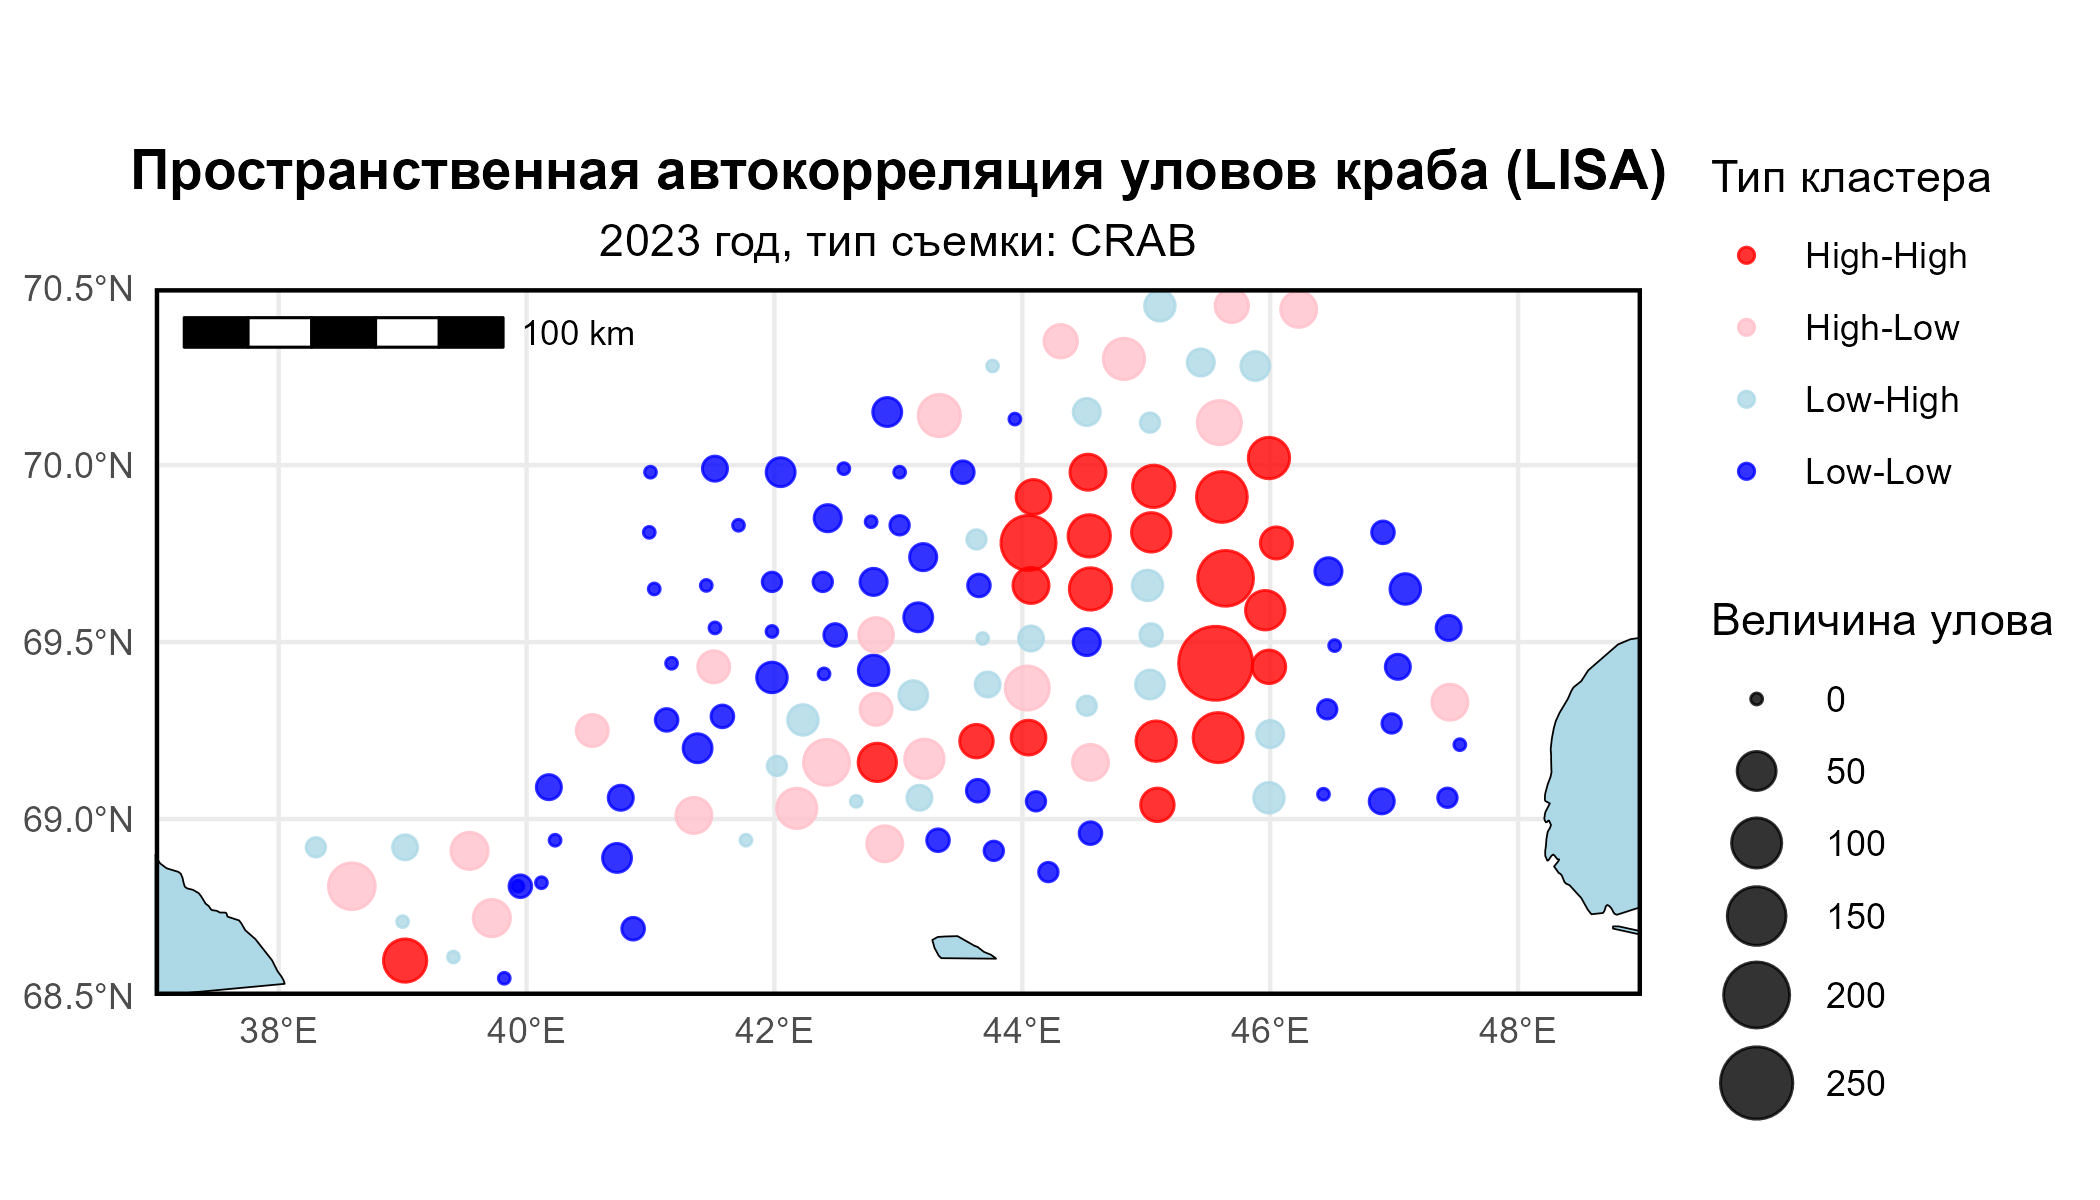
\includegraphics[width=0.8\linewidth,height=\textheight,keepaspectratio]{images/KARTOGRAPH6.PNG}

}

\caption{Рис. 6.: Карта распределения уловов с автокорреляцией LISA}

\end{figure}%

\begin{Shaded}
\begin{Highlighting}[]
\CommentTok{\# Очистка окружения и установка рабочей директории}
\FunctionTok{rm}\NormalTok{(}\AttributeTok{list =} \FunctionTok{ls}\NormalTok{())}
\FunctionTok{setwd}\NormalTok{(}\StringTok{"C:/COURSES/KARTOGRAPH/"}\NormalTok{)}

\CommentTok{\# Загрузка библиотек}
\FunctionTok{library}\NormalTok{(rnaturalearth)}
\FunctionTok{library}\NormalTok{(tidyverse)}
\FunctionTok{library}\NormalTok{(sf)}
\FunctionTok{library}\NormalTok{(spdep)}
\FunctionTok{library}\NormalTok{(ggspatial)}
\FunctionTok{library}\NormalTok{(readxl)}

\CommentTok{\# 1. ЗАГРУЗКА И ПОДГОТОВКА ДАННЫХ}
\NormalTok{DATA }\OtherTok{\textless{}{-}} \FunctionTok{read\_excel}\NormalTok{(}\StringTok{"KARTOGRAPHIC.xlsx"}\NormalTok{, }\AttributeTok{sheet =} \StringTok{"SURVEY"}\NormalTok{) }\SpecialCharTok{\%\textgreater{}\%} 
  \FunctionTok{filter}\NormalTok{(YEAR }\SpecialCharTok{==} \DecValTok{2023}\NormalTok{, SURV }\SpecialCharTok{==} \StringTok{"CRAB"}\NormalTok{)}

\CommentTok{\# Проверка названий колонок}
\FunctionTok{print}\NormalTok{(}\FunctionTok{names}\NormalTok{(DATA))  }\CommentTok{\# Убедитесь, что координаты названы правильно}

\CommentTok{\# Преобразование в пространственные данные (замените X/Y на ваши названия)}
\NormalTok{points\_sf }\OtherTok{\textless{}{-}} \FunctionTok{st\_as\_sf}\NormalTok{(DATA, }\AttributeTok{coords =} \FunctionTok{c}\NormalTok{(}\StringTok{"X"}\NormalTok{, }\StringTok{"Y"}\NormalTok{), }\AttributeTok{crs =} \DecValTok{4326}\NormalTok{)}

\CommentTok{\# 2. ПОЛУЧЕНИЕ КАРТЫ РОССИИ}
\CommentTok{\# Задаем границы области}
\NormalTok{xmin }\OtherTok{\textless{}{-}} \DecValTok{37}
\NormalTok{xmax }\OtherTok{\textless{}{-}} \DecValTok{49}
\NormalTok{ymin }\OtherTok{\textless{}{-}} \FloatTok{68.5}
\NormalTok{ymax }\OtherTok{\textless{}{-}} \FloatTok{70.5}

\CommentTok{\# Создаём ограничивающий прямоугольник}
\NormalTok{bbox }\OtherTok{\textless{}{-}} \FunctionTok{st\_bbox}\NormalTok{(}\FunctionTok{c}\NormalTok{(}\AttributeTok{xmin =}\NormalTok{ xmin, }\AttributeTok{xmax =}\NormalTok{ xmax, }\AttributeTok{ymin =}\NormalTok{ ymin, }\AttributeTok{ymax =}\NormalTok{ ymax), }\AttributeTok{crs =} \DecValTok{4326}\NormalTok{)}
\NormalTok{bbox\_poly }\OtherTok{\textless{}{-}} \FunctionTok{st\_as\_sfc}\NormalTok{(bbox)}

\CommentTok{\# Карта России}
\NormalTok{russia }\OtherTok{\textless{}{-}} \FunctionTok{ne\_countries}\NormalTok{(}\AttributeTok{country =} \StringTok{"Russia"}\NormalTok{, }\AttributeTok{scale =} \DecValTok{10}\NormalTok{) }\SpecialCharTok{\%\textgreater{}\%} 
  \FunctionTok{st\_as\_sf}\NormalTok{() }\SpecialCharTok{\%\textgreater{}\%} 
  \FunctionTok{st\_crop}\NormalTok{(bbox)  }\CommentTok{\# Обрезка без st\_intersection}

\CommentTok{\# 3. ПОДГОТОВКА ТОЧЕК}
\CommentTok{\# Удаление дубликатов по координатам}
\NormalTok{coords }\OtherTok{\textless{}{-}} \FunctionTok{st\_coordinates}\NormalTok{(points\_sf)}
\NormalTok{points\_sf }\OtherTok{\textless{}{-}}\NormalTok{ points\_sf[}\SpecialCharTok{!}\FunctionTok{duplicated}\NormalTok{(coords), , drop }\OtherTok{=} \ConstantTok{FALSE}\NormalTok{]}

\CommentTok{\# Перевод в UTM}
\NormalTok{points\_utm }\OtherTok{\textless{}{-}} \FunctionTok{st\_transform}\NormalTok{(points\_sf, }\AttributeTok{crs =} \DecValTok{32638}\NormalTok{)}

\CommentTok{\# 4. АНАЛИЗ LISA}
\CommentTok{\# Матрица весов}
\NormalTok{knn }\OtherTok{\textless{}{-}} \FunctionTok{knearneigh}\NormalTok{(points\_utm, }\AttributeTok{k =} \DecValTok{4}\NormalTok{)}
\NormalTok{nb }\OtherTok{\textless{}{-}} \FunctionTok{knn2nb}\NormalTok{(knn)}
\NormalTok{listw }\OtherTok{\textless{}{-}} \FunctionTok{nb2listw}\NormalTok{(nb, }\AttributeTok{style =} \StringTok{"W"}\NormalTok{)}

\CommentTok{\# Локальный Моран}
\NormalTok{local\_moran }\OtherTok{\textless{}{-}} \FunctionTok{localmoran}\NormalTok{(points\_utm}\SpecialCharTok{$}\NormalTok{PROM, listw)}

\CommentTok{\# Добавляем кластеры}
\NormalTok{points\_utm }\OtherTok{\textless{}{-}}\NormalTok{ points\_utm }\SpecialCharTok{\%\textgreater{}\%}
  \FunctionTok{mutate}\NormalTok{(}
    \AttributeTok{Local\_I =}\NormalTok{ local\_moran[, }\StringTok{"Ii"}\NormalTok{],}
    \AttributeTok{P\_value =}\NormalTok{ local\_moran[, }\StringTok{"Pr(z != E(Ii))"}\NormalTok{],}
    \AttributeTok{Mean\_PROM =} \FunctionTok{mean}\NormalTok{(PROM, }\AttributeTok{na.rm =} \ConstantTok{TRUE}\NormalTok{),  }\CommentTok{\# Добавляем среднее значение}
    \AttributeTok{Cluster =} \FunctionTok{case\_when}\NormalTok{(}
\NormalTok{      Local\_I }\SpecialCharTok{\textgreater{}} \DecValTok{0} \SpecialCharTok{\&}\NormalTok{ PROM }\SpecialCharTok{\textgreater{}}\NormalTok{ Mean\_PROM }\SpecialCharTok{\textasciitilde{}} \StringTok{"High{-}High"}\NormalTok{,}
\NormalTok{      Local\_I }\SpecialCharTok{\textgreater{}} \DecValTok{0} \SpecialCharTok{\&}\NormalTok{ PROM }\SpecialCharTok{\textless{}=}\NormalTok{ Mean\_PROM }\SpecialCharTok{\textasciitilde{}} \StringTok{"Low{-}Low"}\NormalTok{,  }\CommentTok{\# Включаем PROM == 0}
\NormalTok{      Local\_I }\SpecialCharTok{\textless{}} \DecValTok{0} \SpecialCharTok{\&}\NormalTok{ PROM }\SpecialCharTok{\textgreater{}}\NormalTok{ Mean\_PROM }\SpecialCharTok{\textasciitilde{}} \StringTok{"High{-}Low"}\NormalTok{,}
\NormalTok{      Local\_I }\SpecialCharTok{\textless{}} \DecValTok{0} \SpecialCharTok{\&}\NormalTok{ PROM }\SpecialCharTok{\textless{}=}\NormalTok{ Mean\_PROM }\SpecialCharTok{\textasciitilde{}} \StringTok{"Low{-}High"}\NormalTok{,  }\CommentTok{\# PROM == 0 попадает сюда}
      \ConstantTok{TRUE} \SpecialCharTok{\textasciitilde{}} \StringTok{"Not significant"}
\NormalTok{    )}
\NormalTok{  )}

\CommentTok{\# Обратно в WGS84}
\NormalTok{points\_result }\OtherTok{\textless{}{-}} \FunctionTok{st\_transform}\NormalTok{(points\_utm, }\AttributeTok{crs =} \DecValTok{4326}\NormalTok{)}

\CommentTok{\# 5. ВИЗУАЛИЗАЦИЯ}
\NormalTok{cluster\_colors }\OtherTok{\textless{}{-}} \FunctionTok{c}\NormalTok{(}
  \StringTok{"High{-}High"} \OtherTok{=} \StringTok{"red"}\NormalTok{,}
  \StringTok{"Low{-}Low"} \OtherTok{=} \StringTok{"blue"}\NormalTok{,}
  \StringTok{"High{-}Low"} \OtherTok{=} \StringTok{"pink"}\NormalTok{,}
  \StringTok{"Low{-}High"} \OtherTok{=} \StringTok{"lightblue"}\NormalTok{,}
  \StringTok{"Not significant"} \OtherTok{=} \StringTok{"gray"}
\NormalTok{)}

\FunctionTok{ggplot}\NormalTok{() }\SpecialCharTok{+}
  \CommentTok{\# Карта России}
  \FunctionTok{geom\_sf}\NormalTok{(}\AttributeTok{data =}\NormalTok{ russia, }\AttributeTok{fill =} \StringTok{"lightblue"}\NormalTok{, }\AttributeTok{color =} \StringTok{"black"}\NormalTok{) }\SpecialCharTok{+}
  
  \CommentTok{\# Все точки (включая PROM == 0) — в одном слое}
  \FunctionTok{geom\_sf}\NormalTok{(}
    \AttributeTok{data =}\NormalTok{ points\_result,}
    \FunctionTok{aes}\NormalTok{(}\AttributeTok{color =}\NormalTok{ Cluster, }\AttributeTok{size =}\NormalTok{ PROM),}
    \AttributeTok{alpha =} \FloatTok{0.8}
\NormalTok{  ) }\SpecialCharTok{+}
  
  \CommentTok{\# Настройки координат и масштаба}
  \FunctionTok{coord\_sf}\NormalTok{(}\AttributeTok{xlim =} \FunctionTok{c}\NormalTok{(xmin, xmax), }\AttributeTok{ylim =} \FunctionTok{c}\NormalTok{(ymin, ymax), }\AttributeTok{expand =} \ConstantTok{FALSE}\NormalTok{) }\SpecialCharTok{+}
  \FunctionTok{annotation\_scale}\NormalTok{(}\AttributeTok{location =} \StringTok{"tl"}\NormalTok{, }\AttributeTok{width\_hint =} \FloatTok{0.3}\NormalTok{) }\SpecialCharTok{+}
  
  \CommentTok{\# Цвет и размер}
  \FunctionTok{scale\_color\_manual}\NormalTok{(}\AttributeTok{values =}\NormalTok{ cluster\_colors) }\SpecialCharTok{+}
  \FunctionTok{scale\_size\_continuous}\NormalTok{(}\AttributeTok{range =} \FunctionTok{c}\NormalTok{(}\DecValTok{1}\NormalTok{, }\DecValTok{8}\NormalTok{), }\AttributeTok{name =} \StringTok{"Величина улова"}\NormalTok{) }\SpecialCharTok{+}
  
  \CommentTok{\# Заголовки и тема}
  \FunctionTok{labs}\NormalTok{(}
    \AttributeTok{title =} \StringTok{"Пространственная автокорреляция уловов краба (LISA)"}\NormalTok{,}
    \AttributeTok{subtitle =} \StringTok{"2023 год, тип съемки: CRAB"}\NormalTok{,}
    \AttributeTok{color =} \StringTok{"Тип кластера"}
\NormalTok{  ) }\SpecialCharTok{+}
  
\FunctionTok{theme\_minimal}\NormalTok{() }\SpecialCharTok{+}
  \FunctionTok{theme}\NormalTok{(}
    \AttributeTok{plot.title =} \FunctionTok{element\_text}\NormalTok{(}\AttributeTok{hjust =} \FloatTok{0.5}\NormalTok{, }\AttributeTok{face =} \StringTok{"bold"}\NormalTok{),}
    \AttributeTok{plot.subtitle =} \FunctionTok{element\_text}\NormalTok{(}\AttributeTok{hjust =} \FloatTok{0.5}\NormalTok{),}
    \AttributeTok{legend.position =} \StringTok{"right"}\NormalTok{,}
    \AttributeTok{panel.border =} \FunctionTok{element\_rect}\NormalTok{(}\AttributeTok{colour =} \StringTok{"black"}\NormalTok{, }\AttributeTok{size =} \DecValTok{1}\NormalTok{, }\AttributeTok{fill =} \ConstantTok{NA}\NormalTok{)  }\CommentTok{\# Рамка вокруг карты}
\NormalTok{  )}
\end{Highlighting}
\end{Shaded}

\section{Карта распределения уловов с автокорреляцией LISA по
фасеткам}\label{ux43aux430ux440ux442ux430-ux440ux430ux441ux43fux440ux435ux434ux435ux43bux435ux43dux438ux44f-ux443ux43bux43eux432ux43eux432-ux441-ux430ux432ux442ux43eux43aux43eux440ux440ux435ux43bux44fux446ux438ux435ux439-lisa-ux43fux43e-ux444ux430ux441ux435ux442ux43aux430ux43c}

\begin{figure}[H]

{\centering 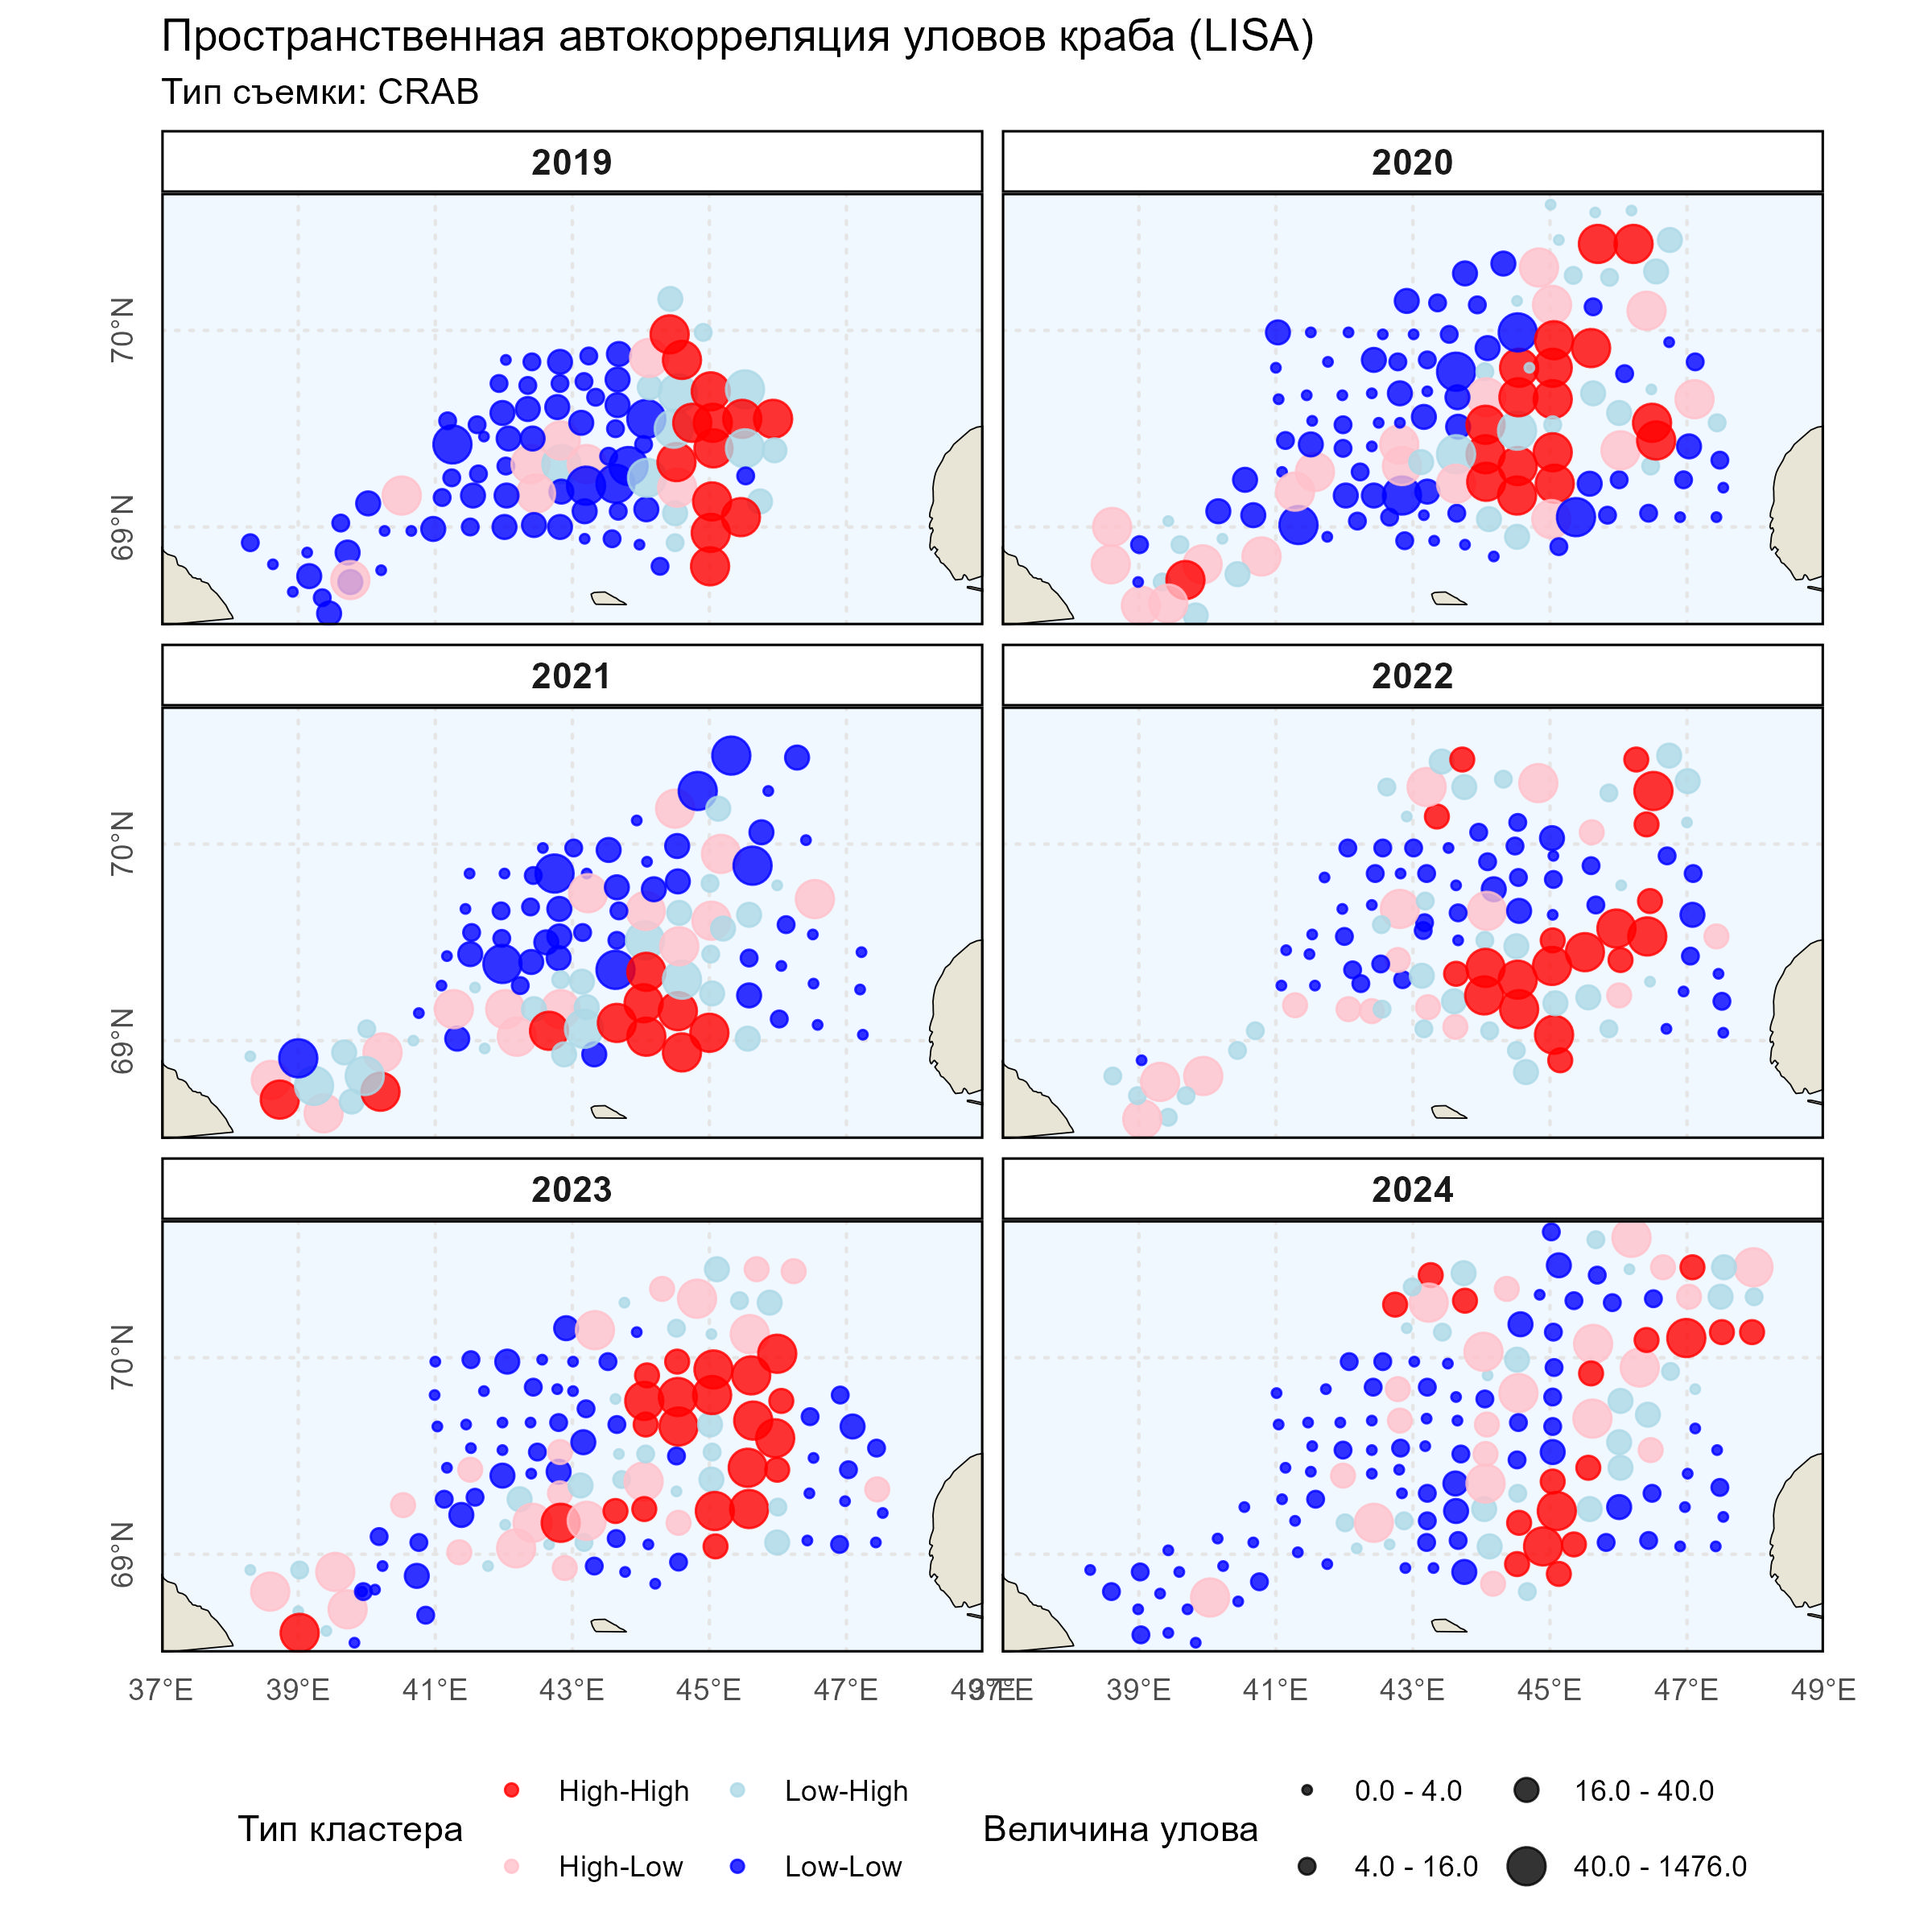
\includegraphics[width=0.8\linewidth,height=\textheight,keepaspectratio]{images/KARTOGRAPH7.PNG}

}

\caption{Рис. 7.: Карта распределения уловов с автокорреляцией LISA по
фасеткам}

\end{figure}%

\begin{Shaded}
\begin{Highlighting}[]
\CommentTok{\# Очистка памяти и установка рабочей папки}
\FunctionTok{rm}\NormalTok{(}\AttributeTok{list =} \FunctionTok{ls}\NormalTok{())}
\FunctionTok{setwd}\NormalTok{(}\StringTok{"C:/COURSES/KARTOGRAPH/"}\NormalTok{)}

\CommentTok{\# Загрузка необходимых пакетов}
\FunctionTok{library}\NormalTok{(rnaturalearth)  }\CommentTok{\# Географические карты}
\FunctionTok{library}\NormalTok{(tidyverse)      }\CommentTok{\# Обработка данных и визуализация}
\FunctionTok{library}\NormalTok{(sf)             }\CommentTok{\# Пространственные данные}
\FunctionTok{library}\NormalTok{(spdep)          }\CommentTok{\# Пространственная статистика}
\FunctionTok{library}\NormalTok{(ggspatial)      }\CommentTok{\# Дополнения для карт в ggplot}
\FunctionTok{library}\NormalTok{(readxl)         }\CommentTok{\# Чтение Excel{-}файлов}

\CommentTok{\# 1. ЗАГРУЗКА И ПРЕОБРАЗОВАНИЕ ДАННЫХ}
\CommentTok{\# {-} Чтение данных из Excel}
\CommentTok{\# {-} Фильтрация только данных по крабу}
\NormalTok{DATA }\OtherTok{\textless{}{-}} \FunctionTok{read\_excel}\NormalTok{(}\StringTok{"KARTOGRAPHIC.xlsx"}\NormalTok{, }\AttributeTok{sheet =} \StringTok{"SURVEY"}\NormalTok{) }\SpecialCharTok{\%\textgreater{}\%} 
  \FunctionTok{filter}\NormalTok{(SURV }\SpecialCharTok{==} \StringTok{"CRAB"}\NormalTok{)}

\CommentTok{\# Преобразование в пространственный объект с координатами}
\NormalTok{points\_sf }\OtherTok{\textless{}{-}} \FunctionTok{st\_as\_sf}\NormalTok{(DATA, }\AttributeTok{coords =} \FunctionTok{c}\NormalTok{(}\StringTok{"X"}\NormalTok{, }\StringTok{"Y"}\NormalTok{), }\AttributeTok{crs =} \DecValTok{4326}\NormalTok{)}

\CommentTok{\# 2. ПОДГОТОВКА КАРТОГРАФИЧЕСКОЙ ОСНОВЫ}
\CommentTok{\# {-} Определение границ области исследования}
\NormalTok{xmin }\OtherTok{\textless{}{-}} \DecValTok{37}\NormalTok{; xmax }\OtherTok{\textless{}{-}} \DecValTok{49}\NormalTok{; ymin }\OtherTok{\textless{}{-}} \FloatTok{68.5}\NormalTok{; ymax }\OtherTok{\textless{}{-}} \FloatTok{70.7}

\CommentTok{\# {-} Создание ограничивающего прямоугольника}
\NormalTok{bbox }\OtherTok{\textless{}{-}} \FunctionTok{st\_bbox}\NormalTok{(}\FunctionTok{c}\NormalTok{(}\AttributeTok{xmin =}\NormalTok{ xmin, }\AttributeTok{xmax =}\NormalTok{ xmax, }\AttributeTok{ymin =}\NormalTok{ ymin, }\AttributeTok{ymax =}\NormalTok{ ymax), }\AttributeTok{crs =} \DecValTok{4326}\NormalTok{)}

\CommentTok{\# {-} Загрузка и обрезка карты России по заданным границам}
\NormalTok{russia }\OtherTok{\textless{}{-}} \FunctionTok{ne\_countries}\NormalTok{(}\AttributeTok{country =} \StringTok{"Russia"}\NormalTok{, }\AttributeTok{scale =} \DecValTok{10}\NormalTok{) }\SpecialCharTok{\%\textgreater{}\%} 
  \FunctionTok{st\_as\_sf}\NormalTok{() }\SpecialCharTok{\%\textgreater{}\%} 
  \FunctionTok{st\_crop}\NormalTok{(bbox)}

\CommentTok{\# 3. ФУНКЦИЯ ДЛЯ ПРОСТРАНСТВЕННОГО АНАЛИЗА ПО ГОДАМ}
\NormalTok{analyze\_year }\OtherTok{\textless{}{-}} \ControlFlowTok{function}\NormalTok{(data\_year) \{}
  \CommentTok{\# Удаление дубликатов координат}
\NormalTok{  coords }\OtherTok{\textless{}{-}} \FunctionTok{st\_coordinates}\NormalTok{(data\_year)}
\NormalTok{  data\_year }\OtherTok{\textless{}{-}}\NormalTok{ data\_year[}\SpecialCharTok{!}\FunctionTok{duplicated}\NormalTok{(coords), , drop }\OtherTok{=} \ConstantTok{FALSE}\NormalTok{]}
  
  \CommentTok{\# Перепроецирование в UTM для точных расчетов}
\NormalTok{  points\_utm }\OtherTok{\textless{}{-}} \FunctionTok{st\_transform}\NormalTok{(data\_year, }\AttributeTok{crs =} \DecValTok{32638}\NormalTok{)}
  
  \CommentTok{\# Построение матрицы пространственных весов (4 ближайших соседа)}
\NormalTok{  knn }\OtherTok{\textless{}{-}} \FunctionTok{knearneigh}\NormalTok{(points\_utm, }\AttributeTok{k =} \DecValTok{4}\NormalTok{)}
\NormalTok{  nb }\OtherTok{\textless{}{-}} \FunctionTok{knn2nb}\NormalTok{(knn)}
\NormalTok{  listw }\OtherTok{\textless{}{-}} \FunctionTok{nb2listw}\NormalTok{(nb, }\AttributeTok{style =} \StringTok{"W"}\NormalTok{)  }\CommentTok{\# Стандартизованная матрица}
  
  \CommentTok{\# Расчет локальной пространственной автокорреляции (LISA)}
\NormalTok{  local\_moran }\OtherTok{\textless{}{-}} \FunctionTok{localmoran}\NormalTok{(points\_utm}\SpecialCharTok{$}\NormalTok{PROM, listw)}
  
  \CommentTok{\# Классификация кластеров на основе результатов}
\NormalTok{  points\_utm }\OtherTok{\textless{}{-}}\NormalTok{ points\_utm }\SpecialCharTok{\%\textgreater{}\%}
    \FunctionTok{mutate}\NormalTok{(}
      \AttributeTok{Local\_I =}\NormalTok{ local\_moran[, }\StringTok{"Ii"}\NormalTok{],}
      \AttributeTok{P\_value =}\NormalTok{ local\_moran[, }\StringTok{"Pr(z != E(Ii))"}\NormalTok{],}
      \AttributeTok{Mean\_PROM =} \FunctionTok{mean}\NormalTok{(PROM, }\AttributeTok{na.rm =} \ConstantTok{TRUE}\NormalTok{),}
      \AttributeTok{Cluster =} \FunctionTok{case\_when}\NormalTok{(}
\NormalTok{        Local\_I }\SpecialCharTok{\textgreater{}} \DecValTok{0} \SpecialCharTok{\&}\NormalTok{ PROM }\SpecialCharTok{\textgreater{}}\NormalTok{ Mean\_PROM }\SpecialCharTok{\textasciitilde{}} \StringTok{"High{-}High"}\NormalTok{,     }\CommentTok{\# Горячая точка}
\NormalTok{        Local\_I }\SpecialCharTok{\textgreater{}} \DecValTok{0} \SpecialCharTok{\&}\NormalTok{ PROM }\SpecialCharTok{\textless{}=}\NormalTok{ Mean\_PROM }\SpecialCharTok{\textasciitilde{}} \StringTok{"Low{-}Low"}\NormalTok{,      }\CommentTok{\# Холодная точка}
\NormalTok{        Local\_I }\SpecialCharTok{\textless{}} \DecValTok{0} \SpecialCharTok{\&}\NormalTok{ PROM }\SpecialCharTok{\textgreater{}}\NormalTok{ Mean\_PROM }\SpecialCharTok{\textasciitilde{}} \StringTok{"High{-}Low"}\NormalTok{,      }\CommentTok{\# Выброс (высокий среди низких)}
\NormalTok{        Local\_I }\SpecialCharTok{\textless{}} \DecValTok{0} \SpecialCharTok{\&}\NormalTok{ PROM }\SpecialCharTok{\textless{}=}\NormalTok{ Mean\_PROM }\SpecialCharTok{\textasciitilde{}} \StringTok{"Low{-}High"}\NormalTok{,     }\CommentTok{\# Выброс (низкий среди высоких)}
        \ConstantTok{TRUE} \SpecialCharTok{\textasciitilde{}} \StringTok{"Not significant"}                          \CommentTok{\# Незначимые}
\NormalTok{      )}
\NormalTok{    )}
  
  \CommentTok{\# Возврат в географические координаты}
  \FunctionTok{st\_transform}\NormalTok{(points\_utm, }\AttributeTok{crs =} \DecValTok{4326}\NormalTok{)}
\NormalTok{\}}

\CommentTok{\# 4. ОБРАБОТКА ДАННЫХ ПО ГОДАМ}
\CommentTok{\# {-} Разделение данных по годам}
\CommentTok{\# {-} Применение анализа для каждого года}
\CommentTok{\# {-} Объединение результатов}
\NormalTok{results\_list }\OtherTok{\textless{}{-}}\NormalTok{ DATA }\SpecialCharTok{\%\textgreater{}\%}
  \FunctionTok{group\_split}\NormalTok{(YEAR) }\SpecialCharTok{\%\textgreater{}\%} 
  \FunctionTok{lapply}\NormalTok{(}\ControlFlowTok{function}\NormalTok{(group) \{}
    \FunctionTok{analyze\_year}\NormalTok{(}\FunctionTok{st\_as\_sf}\NormalTok{(group, }\AttributeTok{coords =} \FunctionTok{c}\NormalTok{(}\StringTok{"X"}\NormalTok{, }\StringTok{"Y"}\NormalTok{), }\AttributeTok{crs =} \DecValTok{4326}\NormalTok{))}
\NormalTok{  \}) }\SpecialCharTok{\%\textgreater{}\%}
  \FunctionTok{bind\_rows}\NormalTok{()}

\CommentTok{\# 5. КАТЕГОРИЗАЦИЯ УЛОВОВ}
\CommentTok{\# {-} Расчет квантилей для всего набора данных}
\NormalTok{PROM\_breaks }\OtherTok{\textless{}{-}} \FunctionTok{quantile}\NormalTok{(results\_list}\SpecialCharTok{$}\NormalTok{PROM, }
                         \AttributeTok{probs =} \FunctionTok{c}\NormalTok{(}\DecValTok{0}\NormalTok{, }\FloatTok{0.25}\NormalTok{, }\FloatTok{0.5}\NormalTok{, }\FloatTok{0.75}\NormalTok{, }\DecValTok{1}\NormalTok{), }
                         \AttributeTok{na.rm =} \ConstantTok{TRUE}\NormalTok{) }\SpecialCharTok{\%\textgreater{}\%} 
  \FunctionTok{round}\NormalTok{(}\DecValTok{1}\NormalTok{)  }\CommentTok{\# Округление значений}

\CommentTok{\# {-} Создание меток с реальными диапазонами}
\NormalTok{PROM\_labels }\OtherTok{\textless{}{-}} \FunctionTok{sprintf}\NormalTok{(}\StringTok{"\%.1f {-} \%.1f"}\NormalTok{, PROM\_breaks[}\DecValTok{1}\SpecialCharTok{:}\DecValTok{4}\NormalTok{], PROM\_breaks[}\DecValTok{2}\SpecialCharTok{:}\DecValTok{5}\NormalTok{])}

\CommentTok{\# {-} Добавление категорий уловов в данные}
\NormalTok{results\_list }\OtherTok{\textless{}{-}}\NormalTok{ results\_list }\SpecialCharTok{\%\textgreater{}\%}
  \FunctionTok{mutate}\NormalTok{(}
    \AttributeTok{PROM\_category =} \FunctionTok{cut}\NormalTok{(}
\NormalTok{      PROM, }
      \AttributeTok{breaks =}\NormalTok{ PROM\_breaks, }
      \AttributeTok{labels =}\NormalTok{ PROM\_labels,}
      \AttributeTok{include.lowest =} \ConstantTok{TRUE}
\NormalTok{    )}
\NormalTok{  )}

\CommentTok{\# 6. ВИЗУАЛИЗАЦИЯ РЕЗУЛЬТАТОВ}
\CommentTok{\# Цветовая схема для типов кластеров}
\NormalTok{cluster\_colors }\OtherTok{\textless{}{-}} \FunctionTok{c}\NormalTok{(}
  \StringTok{"High{-}High"} \OtherTok{=} \StringTok{"red"}\NormalTok{,       }\CommentTok{\# Горячие точки}
  \StringTok{"Low{-}Low"} \OtherTok{=} \StringTok{"blue"}\NormalTok{,        }\CommentTok{\# Холодные точки}
  \StringTok{"High{-}Low"} \OtherTok{=} \StringTok{"pink"}\NormalTok{,       }\CommentTok{\# Выбросы высокие}
  \StringTok{"Low{-}High"} \OtherTok{=} \StringTok{"lightblue"}\NormalTok{,  }\CommentTok{\# Выбросы низкие}
  \StringTok{"Not significant"} \OtherTok{=} \StringTok{"gray"} \CommentTok{\# Незначимые}
\NormalTok{)}

\CommentTok{\# Построение карты}
\FunctionTok{ggplot}\NormalTok{(}\AttributeTok{data =}\NormalTok{ results\_list) }\SpecialCharTok{+}
  \CommentTok{\# Базовая карта России}
  \FunctionTok{geom\_sf}\NormalTok{(}\AttributeTok{data =}\NormalTok{ russia, }\AttributeTok{fill =} \StringTok{"\#E8E5D6"}\NormalTok{, }\AttributeTok{color =} \StringTok{"black"}\NormalTok{, }\AttributeTok{inherit.aes =} \ConstantTok{FALSE}\NormalTok{) }\SpecialCharTok{+}
  
  \CommentTok{\# Точки наблюдений с цветом по кластерам и размером по уловам}
  \FunctionTok{geom\_sf}\NormalTok{(}\FunctionTok{aes}\NormalTok{(}\AttributeTok{color =}\NormalTok{ Cluster, }\AttributeTok{size =}\NormalTok{ PROM\_category), }\AttributeTok{alpha =} \FloatTok{0.8}\NormalTok{) }\SpecialCharTok{+}
  
  \CommentTok{\# Разделение на панели по годам}
  \FunctionTok{facet\_wrap}\NormalTok{(}\SpecialCharTok{\textasciitilde{}}\NormalTok{ YEAR, }\AttributeTok{ncol =} \DecValTok{2}\NormalTok{) }\SpecialCharTok{+}
  
  \CommentTok{\# Установка границ карты}
  \FunctionTok{coord\_sf}\NormalTok{(}\AttributeTok{xlim =} \FunctionTok{c}\NormalTok{(xmin, xmax), }\AttributeTok{ylim =} \FunctionTok{c}\NormalTok{(ymin, ymax), }\AttributeTok{expand =} \ConstantTok{FALSE}\NormalTok{) }\SpecialCharTok{+}
  
  \CommentTok{\# Настройка легенды для кластеров}
  \FunctionTok{scale\_color\_manual}\NormalTok{(}
    \AttributeTok{values =}\NormalTok{ cluster\_colors,}
    \AttributeTok{name =} \StringTok{"Тип кластера"}\NormalTok{,}
    \AttributeTok{guide =} \FunctionTok{guide\_legend}\NormalTok{(}\AttributeTok{nrow =} \DecValTok{2}\NormalTok{)}
\NormalTok{  ) }\SpecialCharTok{+}
  
  \CommentTok{\# Настройка легенды для уловов (реальные диапазоны)}
  \FunctionTok{scale\_size\_manual}\NormalTok{(}
    \AttributeTok{name =} \StringTok{"Величина улова"}\NormalTok{,}
    \AttributeTok{values =} \FunctionTok{c}\NormalTok{(}\DecValTok{1}\NormalTok{, }\DecValTok{2}\NormalTok{, }\DecValTok{3}\NormalTok{, }\DecValTok{5}\NormalTok{),  }\CommentTok{\# Размеры точек для 4{-}х категорий}
    \AttributeTok{breaks =} \FunctionTok{levels}\NormalTok{(results\_list}\SpecialCharTok{$}\NormalTok{PROM\_category),}
    \AttributeTok{guide =} \FunctionTok{guide\_legend}\NormalTok{(}\AttributeTok{nrow =} \DecValTok{2}\NormalTok{)}
\NormalTok{  ) }\SpecialCharTok{+}
  
  \CommentTok{\# Заголовки и подписи}
  \FunctionTok{labs}\NormalTok{(}
    \AttributeTok{title =} \StringTok{"Пространственная автокорреляция уловов краба (LISA)"}\NormalTok{,}
    \AttributeTok{subtitle =} \StringTok{"Тип съемки: CRAB"}
\NormalTok{  ) }\SpecialCharTok{+}
  
  \CommentTok{\# Оформление графика}
  \FunctionTok{theme\_minimal}\NormalTok{() }\SpecialCharTok{+}
  \FunctionTok{theme}\NormalTok{(}
    \AttributeTok{axis.text.x =} \FunctionTok{element\_text}\NormalTok{(}\AttributeTok{size =} \DecValTok{9}\NormalTok{, }\AttributeTok{margin =} \FunctionTok{margin}\NormalTok{(}\AttributeTok{t =} \DecValTok{5}\NormalTok{)),}
    \AttributeTok{axis.text.y =} \FunctionTok{element\_text}\NormalTok{(}\AttributeTok{size =} \DecValTok{9}\NormalTok{, }\AttributeTok{angle =} \DecValTok{90}\NormalTok{, }\AttributeTok{hjust =} \FloatTok{0.5}\NormalTok{, }\AttributeTok{margin =} \FunctionTok{margin}\NormalTok{(}\AttributeTok{r =} \DecValTok{5}\NormalTok{)),}
    \AttributeTok{panel.background =} \FunctionTok{element\_rect}\NormalTok{(}\AttributeTok{fill =} \StringTok{"\#F0F8FF"}\NormalTok{, }\AttributeTok{color =} \ConstantTok{NA}\NormalTok{),  }\CommentTok{\# Фон океана}
    \AttributeTok{panel.grid.major =} \FunctionTok{element\_line}\NormalTok{(}\AttributeTok{color =} \StringTok{"grey90"}\NormalTok{, }\AttributeTok{linetype =} \StringTok{"dotted"}\NormalTok{),}
    \AttributeTok{legend.position =} \StringTok{"bottom"}\NormalTok{,           }\CommentTok{\# Легенда внизу}
    \AttributeTok{legend.box =} \StringTok{"horizontal"}\NormalTok{,            }\CommentTok{\# Горизонтальное расположение}
    \AttributeTok{panel.border =} \FunctionTok{element\_rect}\NormalTok{(}\AttributeTok{fill =} \ConstantTok{NA}\NormalTok{, }\AttributeTok{color =} \StringTok{"black"}\NormalTok{, }\AttributeTok{size =} \FloatTok{0.7}\NormalTok{),}
    \AttributeTok{strip.background =} \FunctionTok{element\_rect}\NormalTok{(}\AttributeTok{fill =} \StringTok{"white"}\NormalTok{, }\AttributeTok{color =} \StringTok{"black"}\NormalTok{, }\AttributeTok{size =} \FloatTok{0.7}\NormalTok{),  }\CommentTok{\# Заголовки панелей}
    \AttributeTok{strip.text =} \FunctionTok{element\_text}\NormalTok{(}\AttributeTok{size =} \DecValTok{11}\NormalTok{, }\AttributeTok{face =} \StringTok{"bold"}\NormalTok{)}
\NormalTok{  ) }\SpecialCharTok{+}
  
  \CommentTok{\# Разметка осей (долгота с шагом 2°, широта с шагом 1°)}
  \FunctionTok{scale\_x\_continuous}\NormalTok{(}
    \AttributeTok{breaks =} \FunctionTok{seq}\NormalTok{(}\FunctionTok{floor}\NormalTok{(xmin), }\FunctionTok{ceiling}\NormalTok{(xmax), }\AttributeTok{by =} \DecValTok{2}\NormalTok{),}
    \AttributeTok{labels =} \ControlFlowTok{function}\NormalTok{(x) }\FunctionTok{paste0}\NormalTok{(x, }\StringTok{"°E"}\NormalTok{)}
\NormalTok{  ) }\SpecialCharTok{+}
  \FunctionTok{scale\_y\_continuous}\NormalTok{(}
    \AttributeTok{breaks =} \FunctionTok{seq}\NormalTok{(}\FunctionTok{floor}\NormalTok{(ymin), }\FunctionTok{ceiling}\NormalTok{(ymax), }\AttributeTok{by =} \DecValTok{1}\NormalTok{),  }
    \AttributeTok{labels =} \ControlFlowTok{function}\NormalTok{(y) }\FunctionTok{paste0}\NormalTok{(y, }\StringTok{"°N"}\NormalTok{)}
\NormalTok{  )}
\end{Highlighting}
\end{Shaded}

\section{Промысловые карты с квартильным распределением
уловов}\label{ux43fux440ux43eux43cux44bux441ux43bux43eux432ux44bux435-ux43aux430ux440ux442ux44b-ux441-ux43aux432ux430ux440ux442ux438ux43bux44cux43dux44bux43c-ux440ux430ux441ux43fux440ux435ux434ux435ux43bux435ux43dux438ux435ux43c-ux443ux43bux43eux432ux43eux432}

\begin{figure}[H]

{\centering 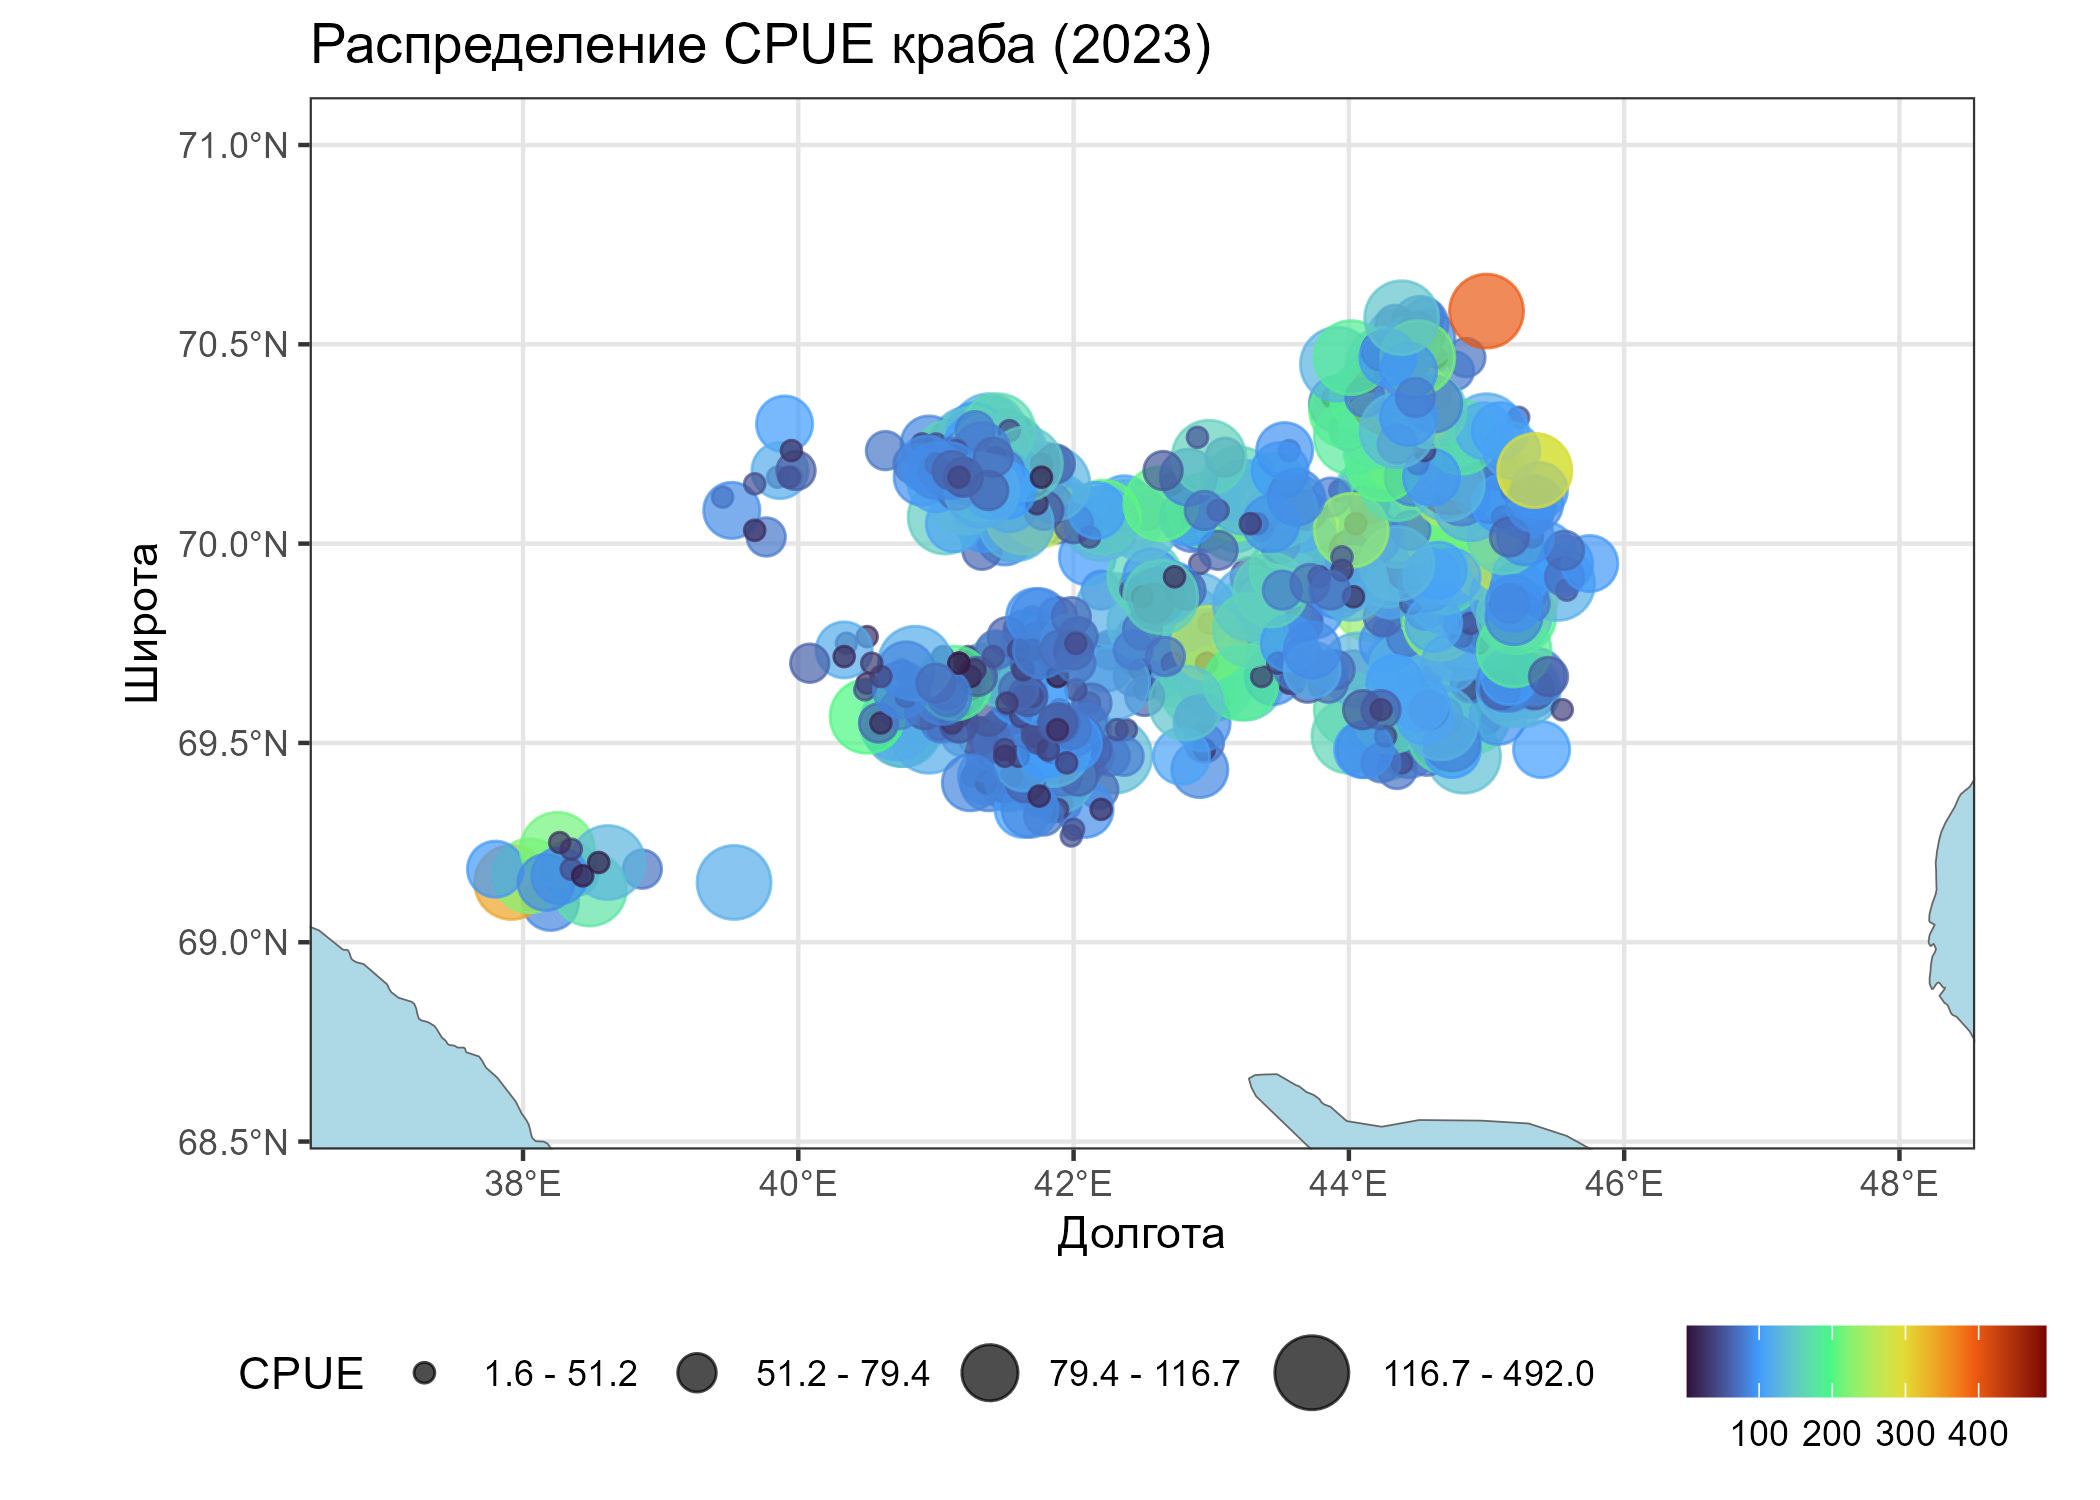
\includegraphics[width=0.8\linewidth,height=\textheight,keepaspectratio]{images/KARTOGRAPH8.PNG}

}

\caption{Рис. 8.: Промысловые карты с квартильным распределением уловов}

\end{figure}%

\begin{Shaded}
\begin{Highlighting}[]
\CommentTok{\# Очистка окружения и установка рабочей директории}
\FunctionTok{rm}\NormalTok{(}\AttributeTok{list =} \FunctionTok{ls}\NormalTok{())}
\FunctionTok{setwd}\NormalTok{(}\StringTok{"C:/COURSES/KARTOGRAPH/"}\NormalTok{)}

\CommentTok{\# Загрузка необходимых библиотек}
\FunctionTok{library}\NormalTok{(rnaturalearth)}
\FunctionTok{library}\NormalTok{(tidyverse)}
\FunctionTok{library}\NormalTok{(sf)}

\DocumentationTok{\#\#\#\#\#\#\# ЗАГРУЗКА ДАННЫХ И ПОДГОТОВКА ПРОСТРАНСТВЕННЫХ ОБЪЕКТОВ \#\#\#\#\#\#\#\#\#\#\#\#\#\#\#\#}

\CommentTok{\# Чтение и фильтрация данных}
\NormalTok{DATA }\OtherTok{\textless{}{-}}\NormalTok{ readxl}\SpecialCharTok{::}\FunctionTok{read\_excel}\NormalTok{(}\StringTok{"KARTOGRAPHIC.xlsx"}\NormalTok{, }\AttributeTok{sheet =} \StringTok{"FISHERY"}\NormalTok{) }\SpecialCharTok{\%\textgreater{}\%} 
  \FunctionTok{filter}\NormalTok{(YEAR }\SpecialCharTok{==} \DecValTok{2023}\NormalTok{)}

\CommentTok{\# Получение границ России}
\NormalTok{russia }\OtherTok{\textless{}{-}} \FunctionTok{ne\_countries}\NormalTok{(}\AttributeTok{scale =} \DecValTok{10}\NormalTok{, }\AttributeTok{country =} \StringTok{"Russia"}\NormalTok{) }\SpecialCharTok{\%\textgreater{}\%} 
  \FunctionTok{st\_as\_sf}\NormalTok{()}

\CommentTok{\# Установка границ отображаемой области}
\NormalTok{xmin}\OtherTok{=}\DecValTok{37}\NormalTok{; xmax}\OtherTok{=}\DecValTok{48}\NormalTok{; ymin}\OtherTok{=}\FloatTok{68.6}\NormalTok{; ymax}\OtherTok{=}\DecValTok{71}

\DocumentationTok{\#\#\#\#\#\#\# ПОДГОТОВКА ДАННЫХ ДЛЯ ВИЗУАЛИЗАЦИИ \#\#\#\#\#\#\#\#\#\#\#\#\#\#\#\#}
\CommentTok{\# Вычисляем квартили отдельно}
\NormalTok{quantiles }\OtherTok{\textless{}{-}} \FunctionTok{quantile}\NormalTok{(DATA}\SpecialCharTok{$}\NormalTok{CPUE[DATA}\SpecialCharTok{$}\NormalTok{CPUE }\SpecialCharTok{\textgreater{}} \DecValTok{0}\NormalTok{], }\AttributeTok{probs =} \FunctionTok{seq}\NormalTok{(}\DecValTok{0}\NormalTok{, }\DecValTok{1}\NormalTok{, }\FloatTok{0.25}\NormalTok{))}

\CommentTok{\# Создаем 4 категории с реальными диапазонами значений}
\NormalTok{nonzero\_data }\OtherTok{\textless{}{-}}\NormalTok{ DATA }\SpecialCharTok{\%\textgreater{}\%} 
  \FunctionTok{filter}\NormalTok{(CPUE }\SpecialCharTok{\textgreater{}} \DecValTok{0}\NormalTok{) }\SpecialCharTok{\%\textgreater{}\%}
  \FunctionTok{mutate}\NormalTok{(}
    \AttributeTok{CPUE\_cat =} \FunctionTok{cut}\NormalTok{(}
\NormalTok{      CPUE,}
      \AttributeTok{breaks =}\NormalTok{ quantiles,}
      \AttributeTok{include.lowest =} \ConstantTok{TRUE}\NormalTok{,}
      \AttributeTok{labels =} \FunctionTok{c}\NormalTok{(}
        \FunctionTok{sprintf}\NormalTok{(}\StringTok{"\%.1f {-} \%.1f"}\NormalTok{, quantiles[}\DecValTok{1}\NormalTok{], quantiles[}\DecValTok{2}\NormalTok{]),}
        \FunctionTok{sprintf}\NormalTok{(}\StringTok{"\%.1f {-} \%.1f"}\NormalTok{, quantiles[}\DecValTok{2}\NormalTok{], quantiles[}\DecValTok{3}\NormalTok{]),}
        \FunctionTok{sprintf}\NormalTok{(}\StringTok{"\%.1f {-} \%.1f"}\NormalTok{, quantiles[}\DecValTok{3}\NormalTok{], quantiles[}\DecValTok{4}\NormalTok{]),}
        \FunctionTok{sprintf}\NormalTok{(}\StringTok{"\%.1f {-} \%.1f"}\NormalTok{, quantiles[}\DecValTok{4}\NormalTok{], quantiles[}\DecValTok{5}\NormalTok{])}
\NormalTok{      )}
\NormalTok{    )}
\NormalTok{  )}

\CommentTok{\# Построение карты}
\FunctionTok{ggplot}\NormalTok{() }\SpecialCharTok{+}
  \CommentTok{\# Базовая карта России}
  \FunctionTok{geom\_sf}\NormalTok{(}\AttributeTok{data =}\NormalTok{ russia, }\AttributeTok{fill =} \StringTok{"lightblue"}\NormalTok{, }\AttributeTok{color =} \StringTok{"gray40"}\NormalTok{) }\SpecialCharTok{+} 
  \CommentTok{\# Ограничение области отображения}
  \FunctionTok{coord\_sf}\NormalTok{(}\AttributeTok{xlim =} \FunctionTok{c}\NormalTok{(xmin, xmax), }\AttributeTok{ylim =} \FunctionTok{c}\NormalTok{(ymin, ymax)) }\SpecialCharTok{+}
  \CommentTok{\# Точки наблюдений с категориальным размером}
  \FunctionTok{geom\_point}\NormalTok{(}
    \AttributeTok{data =}\NormalTok{ nonzero\_data,}
    \FunctionTok{aes}\NormalTok{(}\AttributeTok{x =}\NormalTok{ X, }\AttributeTok{y =}\NormalTok{ Y, }\AttributeTok{size =}\NormalTok{ CPUE\_cat, }\AttributeTok{color =}\NormalTok{ CPUE),}
    \AttributeTok{alpha =} \FloatTok{0.7}
\NormalTok{  ) }\SpecialCharTok{+}
  \CommentTok{\# Точки для нулевых уловов (крестики)}
  \FunctionTok{geom\_point}\NormalTok{(}
    \AttributeTok{data =} \FunctionTok{filter}\NormalTok{(DATA, CPUE }\SpecialCharTok{==} \DecValTok{0}\NormalTok{),}
    \FunctionTok{aes}\NormalTok{(}\AttributeTok{x =}\NormalTok{ X, }\AttributeTok{y =}\NormalTok{ Y),}
    \AttributeTok{shape =} \DecValTok{4}\NormalTok{, }\AttributeTok{size =} \FloatTok{1.2}\NormalTok{, }\AttributeTok{stroke =} \DecValTok{1}\NormalTok{, }\AttributeTok{color =} \StringTok{"black"}
\NormalTok{  ) }\SpecialCharTok{+}
  \CommentTok{\# Цветовая шкала (непрерывная)}
  \FunctionTok{scale\_color\_viridis\_c}\NormalTok{(}\AttributeTok{option =} \StringTok{"H"}\NormalTok{, }\AttributeTok{name =} \ConstantTok{NULL}\NormalTok{) }\SpecialCharTok{+}
  \CommentTok{\# Ручная настройка размеров для категорий}
  \FunctionTok{scale\_size\_manual}\NormalTok{(}
    \AttributeTok{name =} \StringTok{"CPUE"}\NormalTok{,}
    \AttributeTok{values =} \FunctionTok{c}\NormalTok{(}\DecValTok{2}\NormalTok{, }\DecValTok{4}\NormalTok{, }\DecValTok{6}\NormalTok{, }\DecValTok{8}\NormalTok{),  }\CommentTok{\# Размеры точек для категорий}
    \AttributeTok{drop =} \ConstantTok{FALSE}
\NormalTok{  ) }\SpecialCharTok{+}
  \CommentTok{\# Настройки темы}
  \FunctionTok{theme\_bw}\NormalTok{() }\SpecialCharTok{+}
  \FunctionTok{labs}\NormalTok{(}
    \AttributeTok{title =} \StringTok{"Распределение CPUE краба (2023)"}\NormalTok{,}
    \AttributeTok{subtitle =} \ConstantTok{NULL}\NormalTok{,}
    \AttributeTok{x =} \StringTok{"Долгота"}\NormalTok{, }
    \AttributeTok{y =} \StringTok{"Широта"}
\NormalTok{  ) }\SpecialCharTok{+}
  \FunctionTok{theme}\NormalTok{(}
    \AttributeTok{panel.grid =} \FunctionTok{element\_line}\NormalTok{(}\AttributeTok{color =} \StringTok{"gray90"}\NormalTok{),}
    \AttributeTok{legend.position =} \StringTok{"bottom"}
\NormalTok{  )}
\end{Highlighting}
\end{Shaded}

\section{Промысловые карты с агрегацией в центрах полигонов
(промквадратов)}\label{ux43fux440ux43eux43cux44bux441ux43bux43eux432ux44bux435-ux43aux430ux440ux442ux44b-ux441-ux430ux433ux440ux435ux433ux430ux446ux438ux435ux439-ux432-ux446ux435ux43dux442ux440ux430ux445-ux43fux43eux43bux438ux433ux43eux43dux43eux432-ux43fux440ux43eux43cux43aux432ux430ux434ux440ux430ux442ux43eux432}

\begin{figure}[H]

{\centering 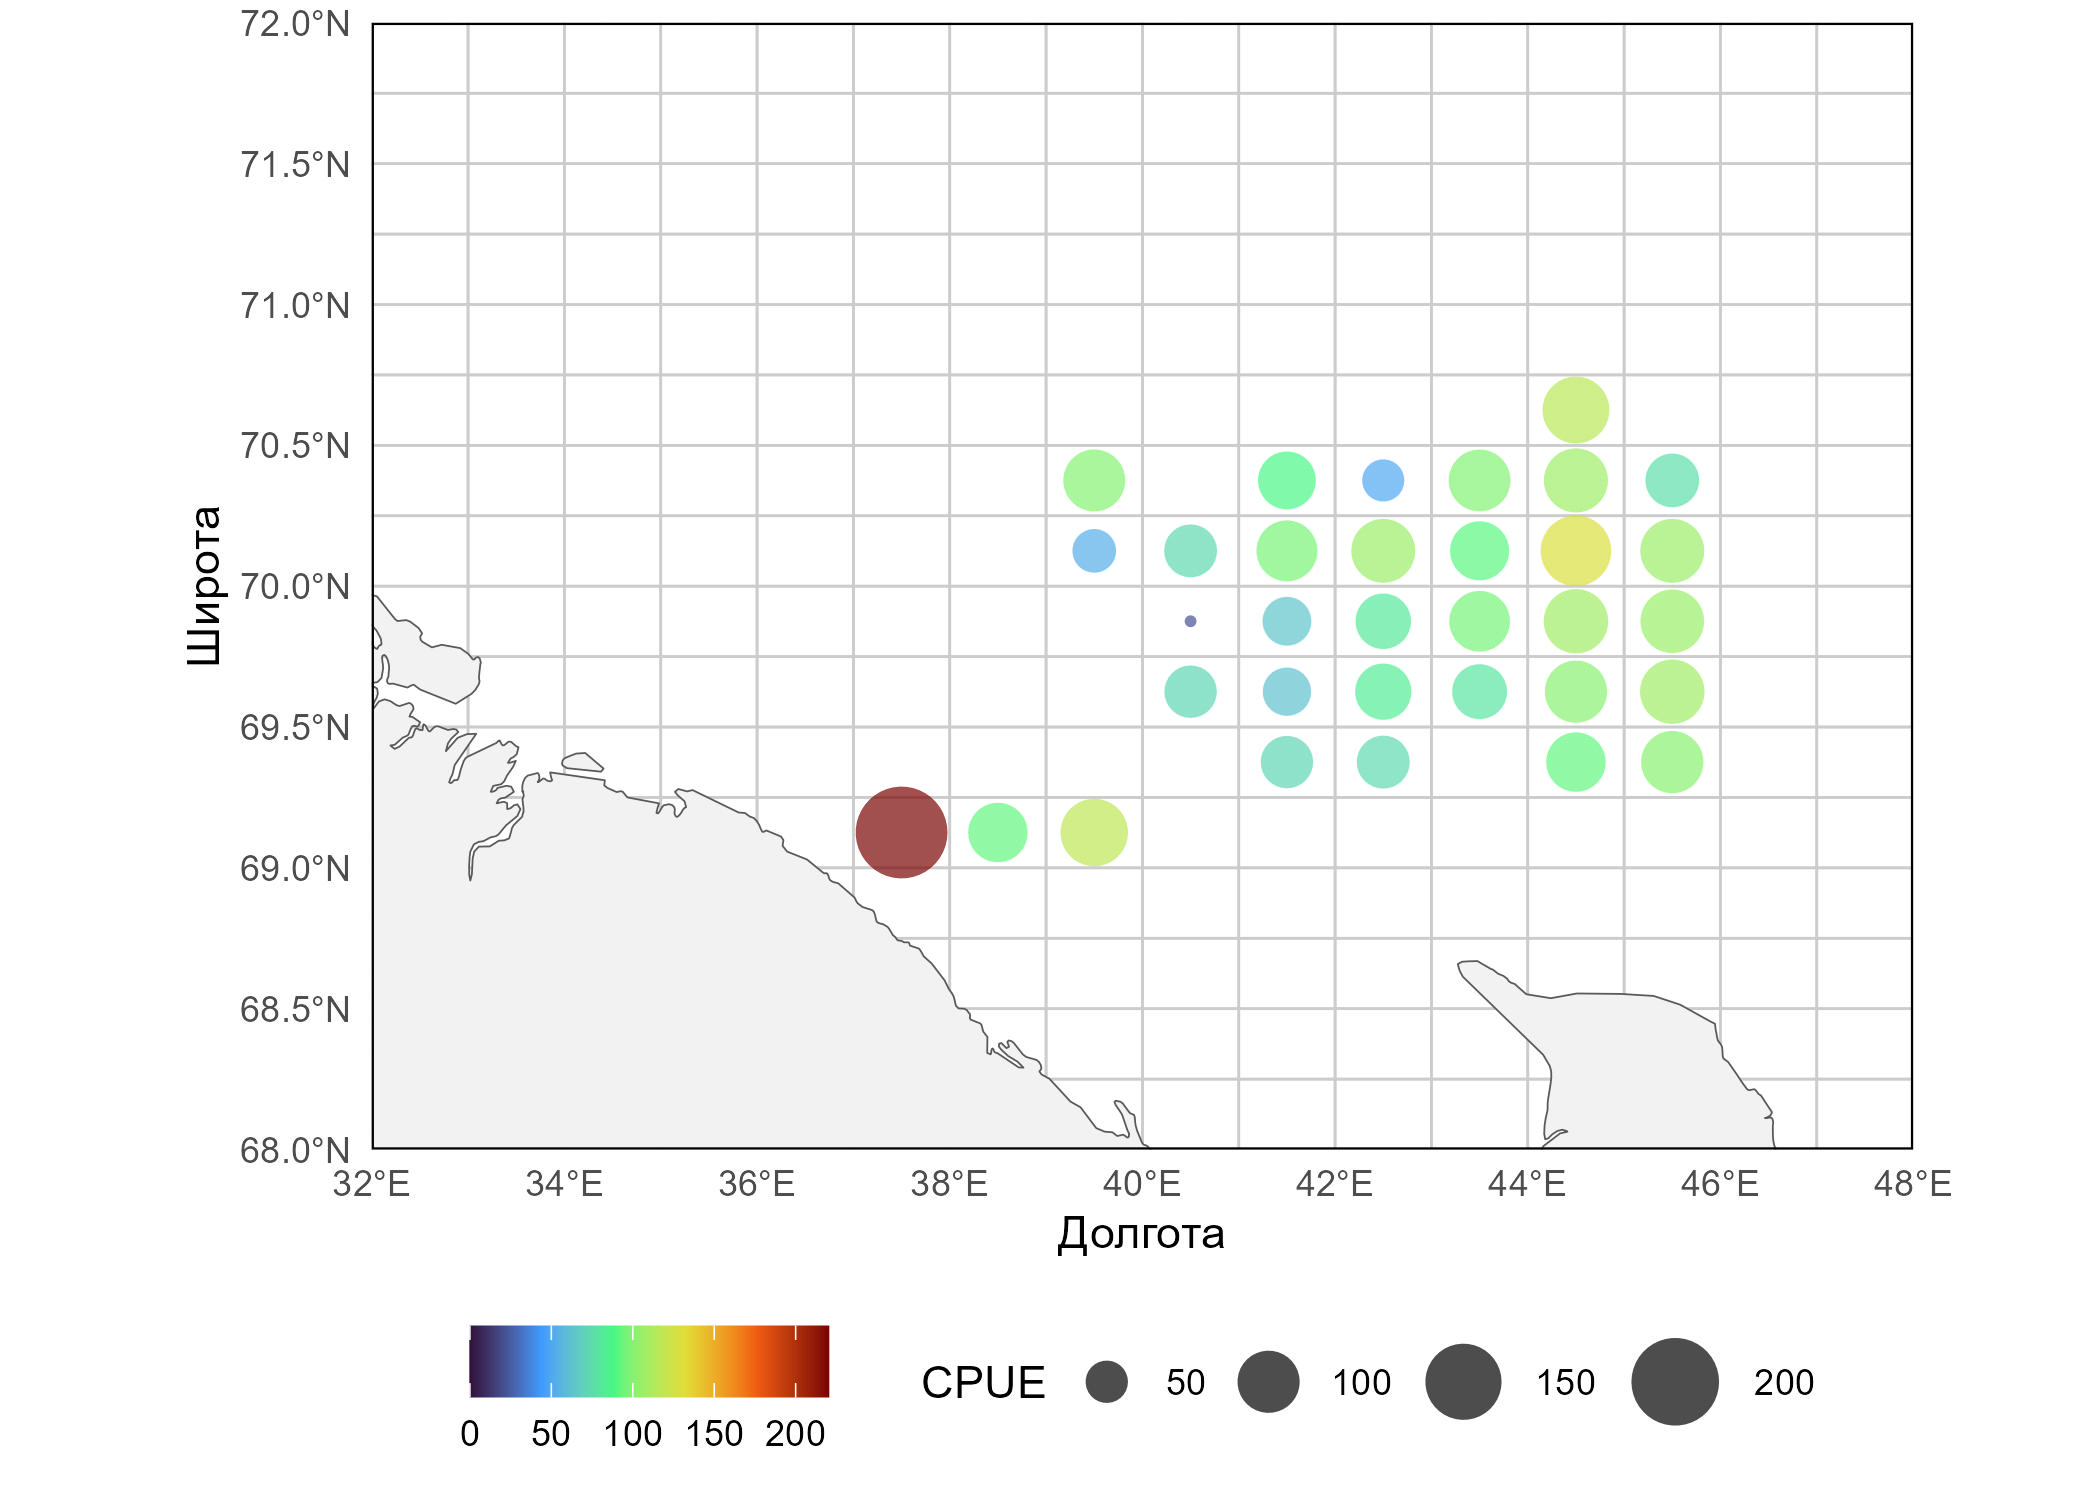
\includegraphics[width=0.8\linewidth,height=\textheight,keepaspectratio]{images/KARTOGRAPH9.PNG}

}

\caption{Рис. 9.: Промысловые карты с агрегацией в центрах полигонов
(промквадратов)}

\end{figure}%

\begin{Shaded}
\begin{Highlighting}[]
\CommentTok{\# Очистка окружения и установка рабочей директории}
\FunctionTok{rm}\NormalTok{(}\AttributeTok{list =} \FunctionTok{ls}\NormalTok{())}
\FunctionTok{setwd}\NormalTok{(}\StringTok{"C:/COURSES/KARTOGRAPH/"}\NormalTok{)}

\CommentTok{\# Загрузка необходимых библиотек}
\FunctionTok{library}\NormalTok{(rnaturalearth)}
\FunctionTok{library}\NormalTok{(tidyverse)}
\FunctionTok{library}\NormalTok{(sf)}

\DocumentationTok{\#\#\#\#\#\#\# ЗАГРУЗКА ДАННЫХ И ПОДГОТОВКА ПРОСТРАНСТВЕННЫХ ОБЪЕКТОВ \#\#\#\#\#\#\#\#\#\#\#\#\#\#\#\#}

\CommentTok{\# Чтение и фильтрация данных}
\NormalTok{DATA }\OtherTok{\textless{}{-}}\NormalTok{ readxl}\SpecialCharTok{::}\FunctionTok{read\_excel}\NormalTok{(}\StringTok{"KARTOGRAPHIC.xlsx"}\NormalTok{, }\AttributeTok{sheet =} \StringTok{"FISHERY"}\NormalTok{) }\SpecialCharTok{\%\textgreater{}\%} 
  \FunctionTok{filter}\NormalTok{(YEAR }\SpecialCharTok{==} \DecValTok{2023}\NormalTok{)}

\CommentTok{\# Преобразуем CPUE в пространственные точки}
\NormalTok{spec\_points }\OtherTok{\textless{}{-}} \FunctionTok{st\_as\_sf}\NormalTok{(DATA, }\AttributeTok{coords =} \FunctionTok{c}\NormalTok{(}\StringTok{"X"}\NormalTok{, }\StringTok{"Y"}\NormalTok{), }\AttributeTok{crs =} \DecValTok{4326}\NormalTok{)}

\CommentTok{\# Карта России}
\NormalTok{russia }\OtherTok{\textless{}{-}} \FunctionTok{ne\_countries}\NormalTok{(}\AttributeTok{scale =} \DecValTok{10}\NormalTok{, }\AttributeTok{country =} \StringTok{"Russia"}\NormalTok{) }

\CommentTok{\# Параметры карты и сетки}
\NormalTok{xmin }\OtherTok{\textless{}{-}} \DecValTok{32}\NormalTok{; xmax }\OtherTok{\textless{}{-}} \DecValTok{48}\NormalTok{; ymin }\OtherTok{\textless{}{-}} \DecValTok{68}\NormalTok{; ymax }\OtherTok{\textless{}{-}} \DecValTok{72}
\NormalTok{xcs }\OtherTok{\textless{}{-}} \DecValTok{1}\NormalTok{; ycs }\OtherTok{\textless{}{-}} \FloatTok{0.25}


\CommentTok{\# Создание основного датафрейма и пространственных объектов}
\NormalTok{points\_sf }\OtherTok{\textless{}{-}} \FunctionTok{st\_as\_sf}\NormalTok{(DATA, }\AttributeTok{coords =} \FunctionTok{c}\NormalTok{(}\StringTok{"X"}\NormalTok{, }\StringTok{"Y"}\NormalTok{), }\AttributeTok{crs =} \DecValTok{4326}\NormalTok{)}

\CommentTok{\# Создание сетки}
\NormalTok{grid\_sf }\OtherTok{\textless{}{-}} \FunctionTok{st\_make\_grid}\NormalTok{(points\_sf, }
                        \AttributeTok{cellsize =} \FunctionTok{c}\NormalTok{(xcs, ycs),}
                        \AttributeTok{n =} \FunctionTok{c}\NormalTok{(}\DecValTok{2} \SpecialCharTok{+}\NormalTok{ (xmax }\SpecialCharTok{{-}}\NormalTok{ xmin)}\SpecialCharTok{/}\NormalTok{xcs, }\DecValTok{2} \SpecialCharTok{+}\NormalTok{ (ymax }\SpecialCharTok{{-}}\NormalTok{ ymin)}\SpecialCharTok{/}\NormalTok{ycs),}
                        \AttributeTok{offset =} \FunctionTok{c}\NormalTok{(xmin }\SpecialCharTok{{-}}\NormalTok{ xcs, ymin }\SpecialCharTok{{-}}\NormalTok{ ycs)) }\SpecialCharTok{\%\textgreater{}\%} 
  \FunctionTok{st\_sf}\NormalTok{() }\SpecialCharTok{\%\textgreater{}\%} 
  \FunctionTok{mutate}\NormalTok{(}\AttributeTok{cell\_id =} \FunctionTok{row\_number}\NormalTok{())}

\CommentTok{\# Присоединяем точки Catch к сетке и агрегируем по ячейкам и годам}
\NormalTok{shares\_df\_catch }\OtherTok{\textless{}{-}} \FunctionTok{st\_join}\NormalTok{(points\_sf, grid\_sf) }\SpecialCharTok{\%\textgreater{}\%} 
  \FunctionTok{st\_drop\_geometry}\NormalTok{() }\SpecialCharTok{\%\textgreater{}\%} 
  \FunctionTok{group\_by}\NormalTok{(cell\_id, YEAR) }\SpecialCharTok{\%\textgreater{}\%} 
  \FunctionTok{summarise}\NormalTok{(}
    \AttributeTok{Count =} \FunctionTok{n}\NormalTok{(),}
    \AttributeTok{CATCH =} \FunctionTok{mean}\NormalTok{(CPUE, }\AttributeTok{na.rm =} \ConstantTok{TRUE}\NormalTok{)}
\NormalTok{  ) }\SpecialCharTok{\%\textgreater{}\%} 
  \FunctionTok{ungroup}\NormalTok{()}

\CommentTok{\# Присоединяем статистику Catch к сетке}
\NormalTok{gird\_shares\_catch }\OtherTok{\textless{}{-}} \FunctionTok{right\_join}\NormalTok{(grid\_sf, shares\_df\_catch, }\AttributeTok{by =} \StringTok{"cell\_id"}\NormalTok{)}



\CommentTok{\# Центроиды сетки по W}
\NormalTok{CENTROIDS\_W }\OtherTok{\textless{}{-}}\NormalTok{ gird\_shares\_catch }\SpecialCharTok{\%\textgreater{}\%} 
  \FunctionTok{st\_centroid}\NormalTok{()}

\DocumentationTok{\#\#\#\#\#\#\#\#\#\#\#\#\#\#\#\#\#\#\#\# ВИЗУАЛИЗАЦИЯ \#\#\#\#\#\#\#\#\#\#\#\#\#\#\#\#\#\#\#\#\#\#\#\#\#\#\#\#\#\#\#\#\#\#\#\#\#\#\#\#\#}

\FunctionTok{ggplot}\NormalTok{() }\SpecialCharTok{+}
  \CommentTok{\# 1. Сетка без заливки}
  \FunctionTok{geom\_sf}\NormalTok{(}\AttributeTok{data =}\NormalTok{ grid\_sf, }\AttributeTok{fill =} \ConstantTok{NA}\NormalTok{, }\AttributeTok{color =} \StringTok{"grey80"}\NormalTok{, }\AttributeTok{linewidth =} \FloatTok{0.3}\NormalTok{) }\SpecialCharTok{+}
  
  \CommentTok{\# 2. Границы России}
  \FunctionTok{geom\_sf}\NormalTok{(}\AttributeTok{data =}\NormalTok{ russia, }\AttributeTok{fill =} \StringTok{"grey95"}\NormalTok{) }\SpecialCharTok{+}
  
  \CommentTok{\# 3. Центроиды ячеек с CATCH (цвет и размер по значению)}
  \FunctionTok{geom\_sf}\NormalTok{(}
    \AttributeTok{data =}\NormalTok{ CENTROIDS\_W, }
    \FunctionTok{aes}\NormalTok{(}\AttributeTok{size =}\NormalTok{ CATCH, }\AttributeTok{color =}\NormalTok{ CATCH),}
    \AttributeTok{shape =} \DecValTok{16}\NormalTok{, }
    \AttributeTok{alpha =} \FloatTok{0.7}
\NormalTok{  ) }\SpecialCharTok{+}
  
  \CommentTok{\# 4. Цветовая шкала (viridis как в первом скрипте)}
  \FunctionTok{scale\_color\_viridis\_c}\NormalTok{(}
    \AttributeTok{option =} \StringTok{"H"}\NormalTok{, }
    \AttributeTok{name =} \ConstantTok{NULL}\NormalTok{,}
    \AttributeTok{limits =} \FunctionTok{c}\NormalTok{(}\DecValTok{0}\NormalTok{, }\FunctionTok{max}\NormalTok{(gird\_shares\_catch}\SpecialCharTok{$}\NormalTok{CATCH, }\AttributeTok{na.rm =} \ConstantTok{TRUE}\NormalTok{))}
\NormalTok{  ) }\SpecialCharTok{+}
  
  \CommentTok{\# 5. Шкала размера центроидов}
  \FunctionTok{scale\_size\_continuous}\NormalTok{(}
    \AttributeTok{range =} \FunctionTok{c}\NormalTok{(}\DecValTok{1}\NormalTok{, }\DecValTok{10}\NormalTok{), }
    \AttributeTok{name =} \StringTok{"CPUE"}
\NormalTok{  ) }\SpecialCharTok{+}
  
  \CommentTok{\# 6. Обрезаем область отображения}
  \FunctionTok{coord\_sf}\NormalTok{(}
    \AttributeTok{xlim =} \FunctionTok{c}\NormalTok{(xmin, xmax), }
    \AttributeTok{ylim =} \FunctionTok{c}\NormalTok{(ymin, ymax),}
    \AttributeTok{expand =} \ConstantTok{FALSE}  \CommentTok{\# Точное соответствие границ}
\NormalTok{  ) }\SpecialCharTok{+}
  
  \CommentTok{\# 7. Шкалы для осей координат}
  \FunctionTok{scale\_x\_continuous}\NormalTok{(}
    \AttributeTok{breaks =} \FunctionTok{seq}\NormalTok{(xmin, xmax, }\AttributeTok{by =} \DecValTok{2}\NormalTok{),  }\CommentTok{\# Метки каждые 2 градуса}
    \AttributeTok{name =} \StringTok{"Долгота"}
\NormalTok{  ) }\SpecialCharTok{+}
  \FunctionTok{scale\_y\_continuous}\NormalTok{(}
    \AttributeTok{breaks =} \FunctionTok{seq}\NormalTok{(ymin, ymax, }\AttributeTok{by =} \FloatTok{0.5}\NormalTok{),  }\CommentTok{\# Метки каждые 0.5 градуса}
    \AttributeTok{name =} \StringTok{"Широта"}
\NormalTok{  ) }\SpecialCharTok{+}
  
  \CommentTok{\# 8. Тема оформления}
  \FunctionTok{theme\_minimal}\NormalTok{() }\SpecialCharTok{+}
  \FunctionTok{theme}\NormalTok{(}
    \AttributeTok{panel.grid =} \FunctionTok{element\_blank}\NormalTok{(),}
    \AttributeTok{legend.position =} \StringTok{"bottom"}\NormalTok{,}
    \AttributeTok{panel.border =} \FunctionTok{element\_rect}\NormalTok{(}\AttributeTok{fill =} \ConstantTok{NA}\NormalTok{, }\AttributeTok{color =} \StringTok{"black"}\NormalTok{, }\AttributeTok{size =} \FloatTok{0.5}\NormalTok{),}
    \CommentTok{\# Добавляем сетку для осей координат}
    \AttributeTok{panel.grid.major =} \FunctionTok{element\_line}\NormalTok{(}\AttributeTok{color =} \StringTok{"gray90"}\NormalTok{, }\AttributeTok{linewidth =} \FloatTok{0.2}\NormalTok{)}
\NormalTok{  ) }\SpecialCharTok{+}
  
  \CommentTok{\# 9. Явное указание названий осей (дублируем для надежности)}
  \FunctionTok{labs}\NormalTok{(}\AttributeTok{x =} \StringTok{"Долгота"}\NormalTok{, }\AttributeTok{y =} \StringTok{"Широта"}\NormalTok{)}
\end{Highlighting}
\end{Shaded}

\section{Промысловые карты -
картограммы}\label{ux43fux440ux43eux43cux44bux441ux43bux43eux432ux44bux435-ux43aux430ux440ux442ux44b---ux43aux430ux440ux442ux43eux433ux440ux430ux43cux43cux44b}

\begin{figure}[H]

{\centering 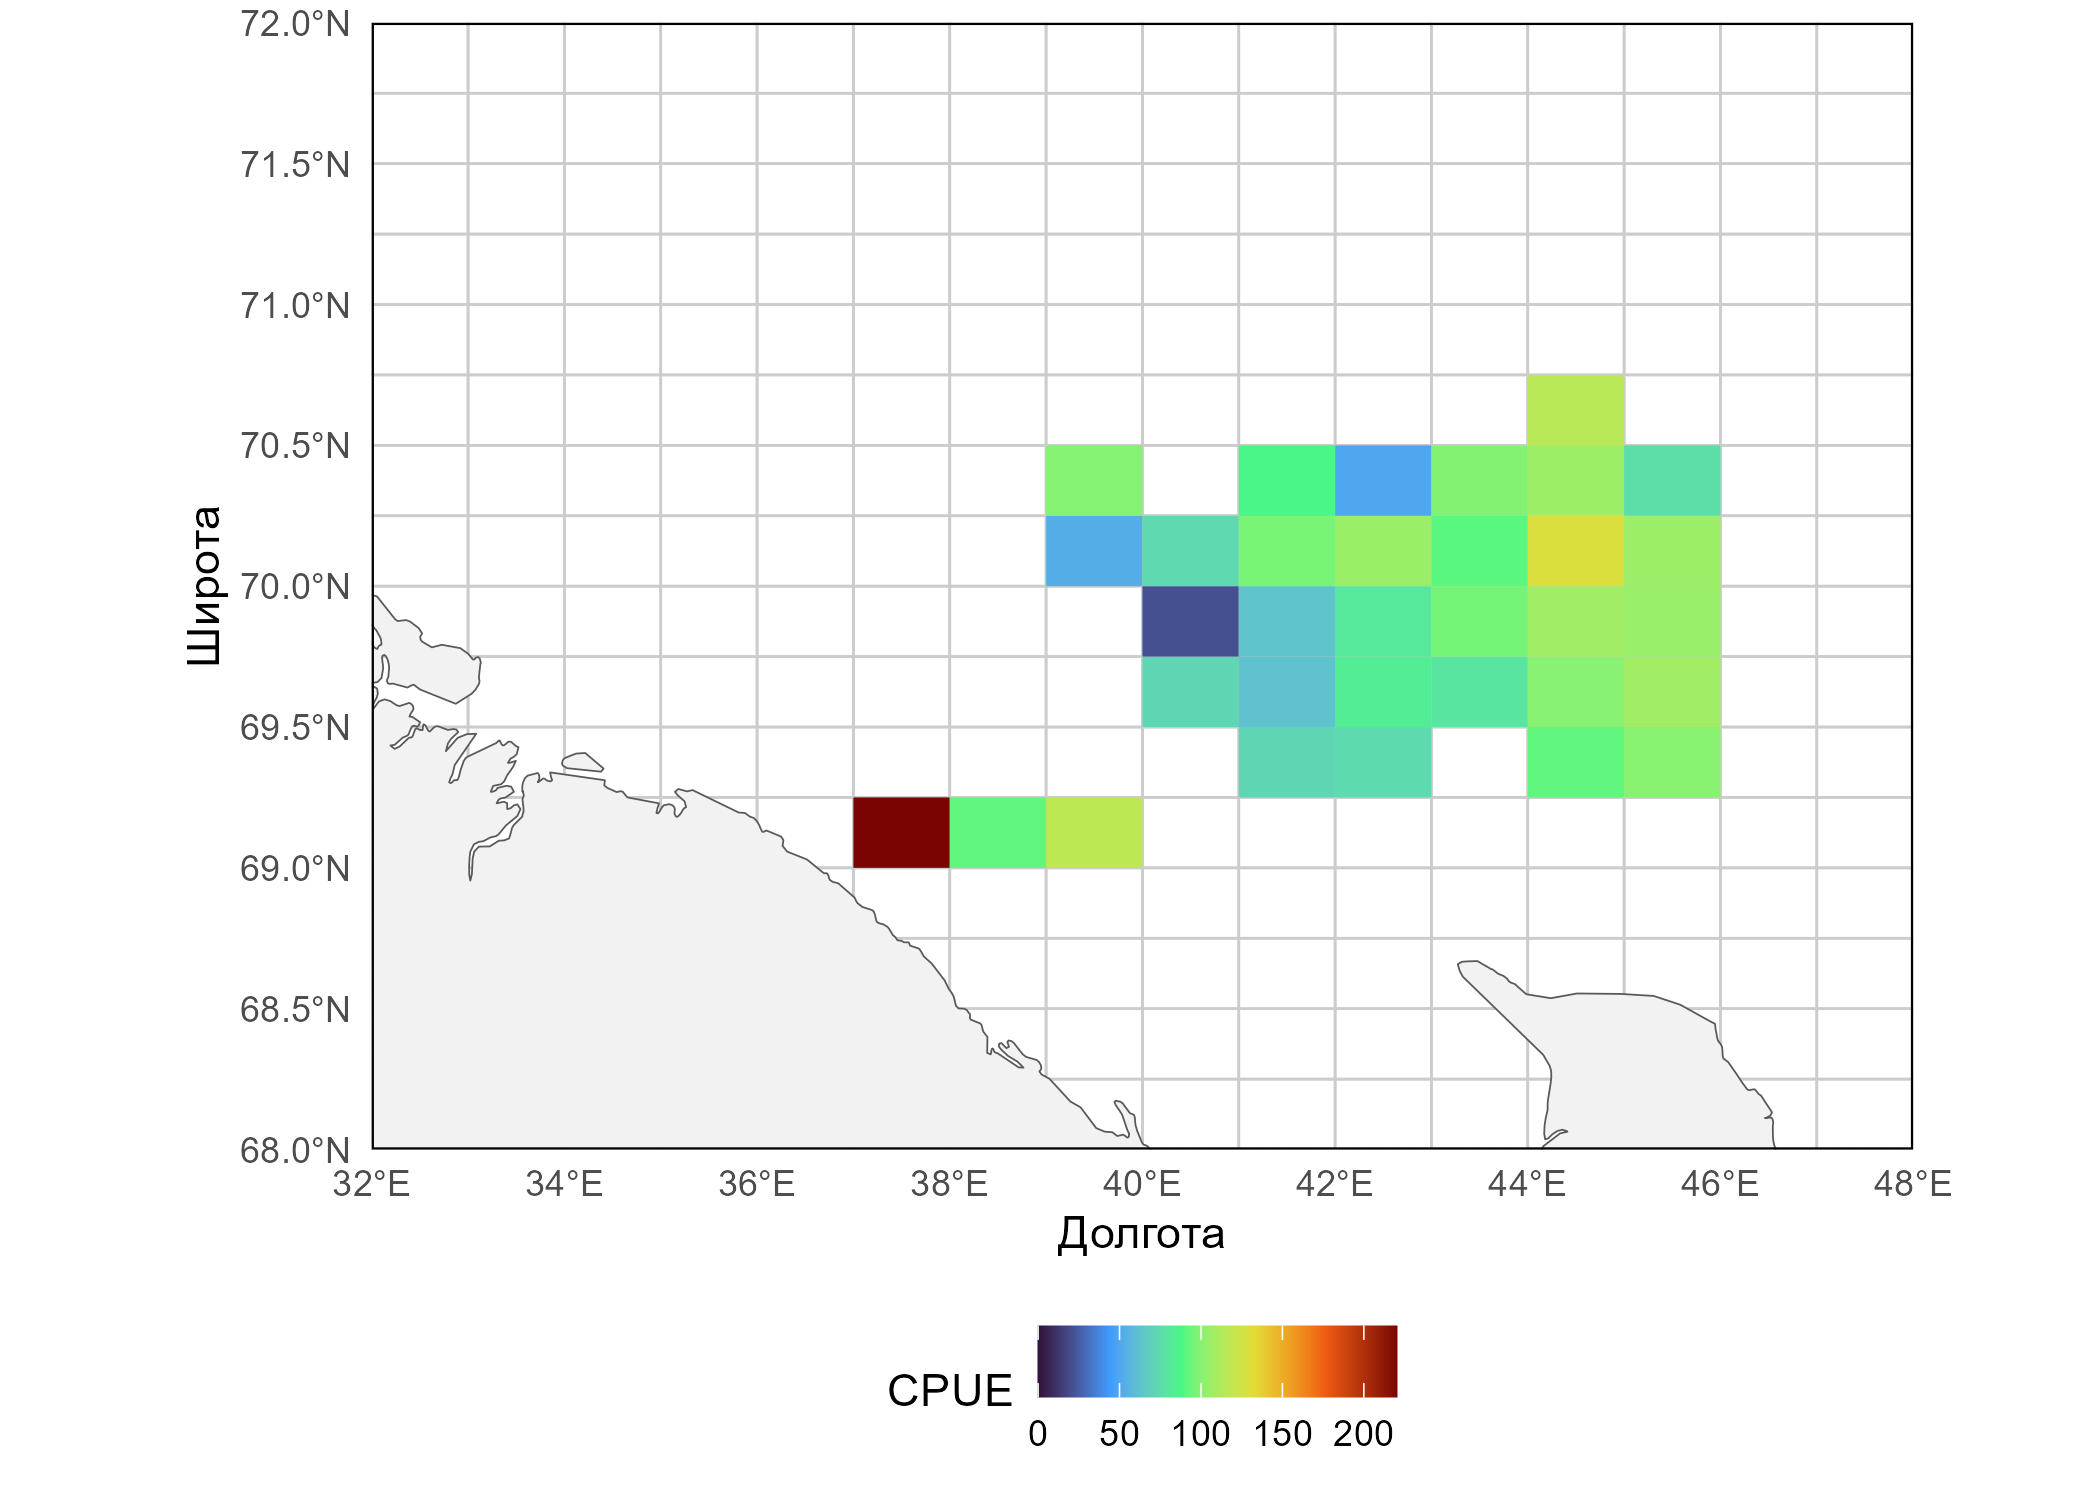
\includegraphics[width=0.8\linewidth,height=\textheight,keepaspectratio]{images/KARTOGRAPH10.PNG}

}

\caption{Рис. 10.: Промысловые карты - картограммы}

\end{figure}%

\begin{Shaded}
\begin{Highlighting}[]
\CommentTok{\# Очистка окружения и установка рабочей директории}
\FunctionTok{rm}\NormalTok{(}\AttributeTok{list =} \FunctionTok{ls}\NormalTok{())}
\FunctionTok{setwd}\NormalTok{(}\StringTok{"C:/COURSES/KARTOGRAPH/"}\NormalTok{)}

\CommentTok{\# Загрузка необходимых библиотек}
\FunctionTok{library}\NormalTok{(rnaturalearth)}
\FunctionTok{library}\NormalTok{(tidyverse)}
\FunctionTok{library}\NormalTok{(sf)}

\DocumentationTok{\#\#\#\#\#\#\# ЗАГРУЗКА ДАННЫХ И ПОДГОТОВКА ПРОСТРАНСТВЕННЫХ ОБЪЕКТОВ \#\#\#\#\#\#\#\#\#\#\#\#\#\#\#\#}

\CommentTok{\# Чтение и фильтрация данных}
\NormalTok{DATA }\OtherTok{\textless{}{-}}\NormalTok{ readxl}\SpecialCharTok{::}\FunctionTok{read\_excel}\NormalTok{(}\StringTok{"KARTOGRAPHIC.xlsx"}\NormalTok{, }\AttributeTok{sheet =} \StringTok{"FISHERY"}\NormalTok{) }\SpecialCharTok{\%\textgreater{}\%} 
  \FunctionTok{filter}\NormalTok{(YEAR }\SpecialCharTok{==} \DecValTok{2023}\NormalTok{)}

\CommentTok{\# Преобразуем CPUE в пространственные точки}
\NormalTok{spec\_points }\OtherTok{\textless{}{-}} \FunctionTok{st\_as\_sf}\NormalTok{(DATA, }\AttributeTok{coords =} \FunctionTok{c}\NormalTok{(}\StringTok{"X"}\NormalTok{, }\StringTok{"Y"}\NormalTok{), }\AttributeTok{crs =} \DecValTok{4326}\NormalTok{)}

\CommentTok{\# Карта России}
\NormalTok{russia }\OtherTok{\textless{}{-}} \FunctionTok{ne\_countries}\NormalTok{(}\AttributeTok{scale =} \DecValTok{10}\NormalTok{, }\AttributeTok{country =} \StringTok{"Russia"}\NormalTok{) }

\CommentTok{\# Параметры карты и сетки}
\NormalTok{xmin }\OtherTok{\textless{}{-}} \DecValTok{32}\NormalTok{; xmax }\OtherTok{\textless{}{-}} \DecValTok{48}\NormalTok{; ymin }\OtherTok{\textless{}{-}} \DecValTok{68}\NormalTok{; ymax }\OtherTok{\textless{}{-}} \DecValTok{72}
\NormalTok{xcs }\OtherTok{\textless{}{-}} \DecValTok{1}\NormalTok{; ycs }\OtherTok{\textless{}{-}} \FloatTok{0.25}


\CommentTok{\# Создание основного датафрейма и пространственных объектов}
\NormalTok{points\_sf }\OtherTok{\textless{}{-}} \FunctionTok{st\_as\_sf}\NormalTok{(DATA, }\AttributeTok{coords =} \FunctionTok{c}\NormalTok{(}\StringTok{"X"}\NormalTok{, }\StringTok{"Y"}\NormalTok{), }\AttributeTok{crs =} \DecValTok{4326}\NormalTok{)}

\CommentTok{\# Создание сетки}
\NormalTok{grid\_sf }\OtherTok{\textless{}{-}} \FunctionTok{st\_make\_grid}\NormalTok{(points\_sf, }
                        \AttributeTok{cellsize =} \FunctionTok{c}\NormalTok{(xcs, ycs),}
                        \AttributeTok{n =} \FunctionTok{c}\NormalTok{(}\DecValTok{2} \SpecialCharTok{+}\NormalTok{ (xmax }\SpecialCharTok{{-}}\NormalTok{ xmin)}\SpecialCharTok{/}\NormalTok{xcs, }\DecValTok{2} \SpecialCharTok{+}\NormalTok{ (ymax }\SpecialCharTok{{-}}\NormalTok{ ymin)}\SpecialCharTok{/}\NormalTok{ycs),}
                        \AttributeTok{offset =} \FunctionTok{c}\NormalTok{(xmin }\SpecialCharTok{{-}}\NormalTok{ xcs, ymin }\SpecialCharTok{{-}}\NormalTok{ ycs)) }\SpecialCharTok{\%\textgreater{}\%} 
  \FunctionTok{st\_sf}\NormalTok{() }\SpecialCharTok{\%\textgreater{}\%} 
  \FunctionTok{mutate}\NormalTok{(}\AttributeTok{cell\_id =} \FunctionTok{row\_number}\NormalTok{())}

\CommentTok{\# Присоединяем точки Catch к сетке и агрегируем по ячейкам и годам}
\NormalTok{shares\_df\_catch }\OtherTok{\textless{}{-}} \FunctionTok{st\_join}\NormalTok{(points\_sf, grid\_sf) }\SpecialCharTok{\%\textgreater{}\%} 
  \FunctionTok{st\_drop\_geometry}\NormalTok{() }\SpecialCharTok{\%\textgreater{}\%} 
  \FunctionTok{group\_by}\NormalTok{(cell\_id, YEAR) }\SpecialCharTok{\%\textgreater{}\%} 
  \FunctionTok{summarise}\NormalTok{(}
    \AttributeTok{Count =} \FunctionTok{n}\NormalTok{(),}
    \AttributeTok{CATCH =} \FunctionTok{mean}\NormalTok{(CPUE, }\AttributeTok{na.rm =} \ConstantTok{TRUE}\NormalTok{)}
\NormalTok{  ) }\SpecialCharTok{\%\textgreater{}\%} 
  \FunctionTok{ungroup}\NormalTok{()}

\CommentTok{\# Присоединяем статистику Catch к сетке}
\NormalTok{gird\_shares\_catch }\OtherTok{\textless{}{-}} \FunctionTok{right\_join}\NormalTok{(grid\_sf, shares\_df\_catch, }\AttributeTok{by =} \StringTok{"cell\_id"}\NormalTok{)}



\CommentTok{\# Центроиды сетки по W}
\NormalTok{CENTROIDS\_W }\OtherTok{\textless{}{-}}\NormalTok{ gird\_shares\_catch }\SpecialCharTok{\%\textgreater{}\%} 
  \FunctionTok{st\_centroid}\NormalTok{()}

\DocumentationTok{\#\#\#\#\#\#\#\#\#\#\#\#\#\#\#\#\#\#\#\# ВИЗУАЛИЗАЦИЯ \#\#\#\#\#\#\#\#\#\#\#\#\#\#\#\#\#\#\#\#\#\#\#\#\#\#\#\#\#\#\#\#\#\#\#\#\#\#\#\#\#}

\FunctionTok{ggplot}\NormalTok{() }\SpecialCharTok{+}
  \CommentTok{\# 1. Сетка без заливки}
  \FunctionTok{geom\_sf}\NormalTok{(}\AttributeTok{data =}\NormalTok{ grid\_sf, }\AttributeTok{fill =} \ConstantTok{NA}\NormalTok{, }\AttributeTok{color =} \StringTok{"grey80"}\NormalTok{, }\AttributeTok{linewidth =} \FloatTok{0.3}\NormalTok{) }\SpecialCharTok{+}
  
  \CommentTok{\# 2. Границы России}
  \FunctionTok{geom\_sf}\NormalTok{(}\AttributeTok{data =}\NormalTok{ russia, }\AttributeTok{fill =} \StringTok{"grey95"}\NormalTok{) }\SpecialCharTok{+}
  
  \CommentTok{\# 3. Заливка по улову с палитрой viridis option "H"}
  \FunctionTok{geom\_sf}\NormalTok{(}\AttributeTok{data =}\NormalTok{ gird\_shares\_catch, }\FunctionTok{aes}\NormalTok{(}\AttributeTok{fill =}\NormalTok{ CATCH), }\AttributeTok{color =} \ConstantTok{NA}\NormalTok{) }\SpecialCharTok{+}
  
  \CommentTok{\# 4. Цветовая шкала viridis option "H" для заливки}
  \FunctionTok{scale\_fill\_viridis\_c}\NormalTok{(}
    \AttributeTok{option =} \StringTok{"H"}\NormalTok{, }
    \AttributeTok{name =} \StringTok{"CPUE"}\NormalTok{,}
    \AttributeTok{limits =} \FunctionTok{c}\NormalTok{(}\DecValTok{0}\NormalTok{, }\FunctionTok{max}\NormalTok{(gird\_shares\_catch}\SpecialCharTok{$}\NormalTok{CATCH, }\AttributeTok{na.rm =} \ConstantTok{TRUE}\NormalTok{)),}
    \AttributeTok{na.value =} \StringTok{"transparent"}
\NormalTok{  ) }\SpecialCharTok{+}
  
  \CommentTok{\# 5. Обрезаем область отображения}
  \FunctionTok{coord\_sf}\NormalTok{(}
    \AttributeTok{xlim =} \FunctionTok{c}\NormalTok{(xmin, xmax), }
    \AttributeTok{ylim =} \FunctionTok{c}\NormalTok{(ymin, ymax),}
    \AttributeTok{expand =} \ConstantTok{FALSE}
\NormalTok{  ) }\SpecialCharTok{+}
  
  \CommentTok{\# 6. Шкалы для осей координат}
  \FunctionTok{scale\_x\_continuous}\NormalTok{(}
    \AttributeTok{breaks =} \FunctionTok{seq}\NormalTok{(xmin, xmax, }\AttributeTok{by =} \DecValTok{2}\NormalTok{),}
    \AttributeTok{name =} \StringTok{"Долгота"}
\NormalTok{  ) }\SpecialCharTok{+}
  \FunctionTok{scale\_y\_continuous}\NormalTok{(}
    \AttributeTok{breaks =} \FunctionTok{seq}\NormalTok{(ymin, ymax, }\AttributeTok{by =} \FloatTok{0.5}\NormalTok{),}
    \AttributeTok{name =} \StringTok{"Широта"}
\NormalTok{  ) }\SpecialCharTok{+}
  
  \CommentTok{\# 7. Тема оформления}
  \FunctionTok{theme\_minimal}\NormalTok{() }\SpecialCharTok{+}
  \FunctionTok{theme}\NormalTok{(}
    \AttributeTok{panel.grid =} \FunctionTok{element\_blank}\NormalTok{(),}
    \AttributeTok{legend.position =} \StringTok{"bottom"}\NormalTok{,}
    \AttributeTok{panel.border =} \FunctionTok{element\_rect}\NormalTok{(}\AttributeTok{fill =} \ConstantTok{NA}\NormalTok{, }\AttributeTok{color =} \StringTok{"black"}\NormalTok{, }\AttributeTok{size =} \FloatTok{0.5}\NormalTok{),}
    \AttributeTok{panel.grid.major =} \FunctionTok{element\_line}\NormalTok{(}\AttributeTok{color =} \StringTok{"gray90"}\NormalTok{, }\AttributeTok{size =} \FloatTok{0.2}\NormalTok{)}
\NormalTok{  ) }\SpecialCharTok{+}
  \FunctionTok{labs}\NormalTok{(}\AttributeTok{x =} \StringTok{"Долгота"}\NormalTok{, }\AttributeTok{y =} \StringTok{"Широта"}\NormalTok{)}
\end{Highlighting}
\end{Shaded}

\section{Промысловые карты - картограммы по
фасеткам}\label{ux43fux440ux43eux43cux44bux441ux43bux43eux432ux44bux435-ux43aux430ux440ux442ux44b---ux43aux430ux440ux442ux43eux433ux440ux430ux43cux43cux44b-ux43fux43e-ux444ux430ux441ux435ux442ux43aux430ux43c}

\begin{figure}[H]

{\centering 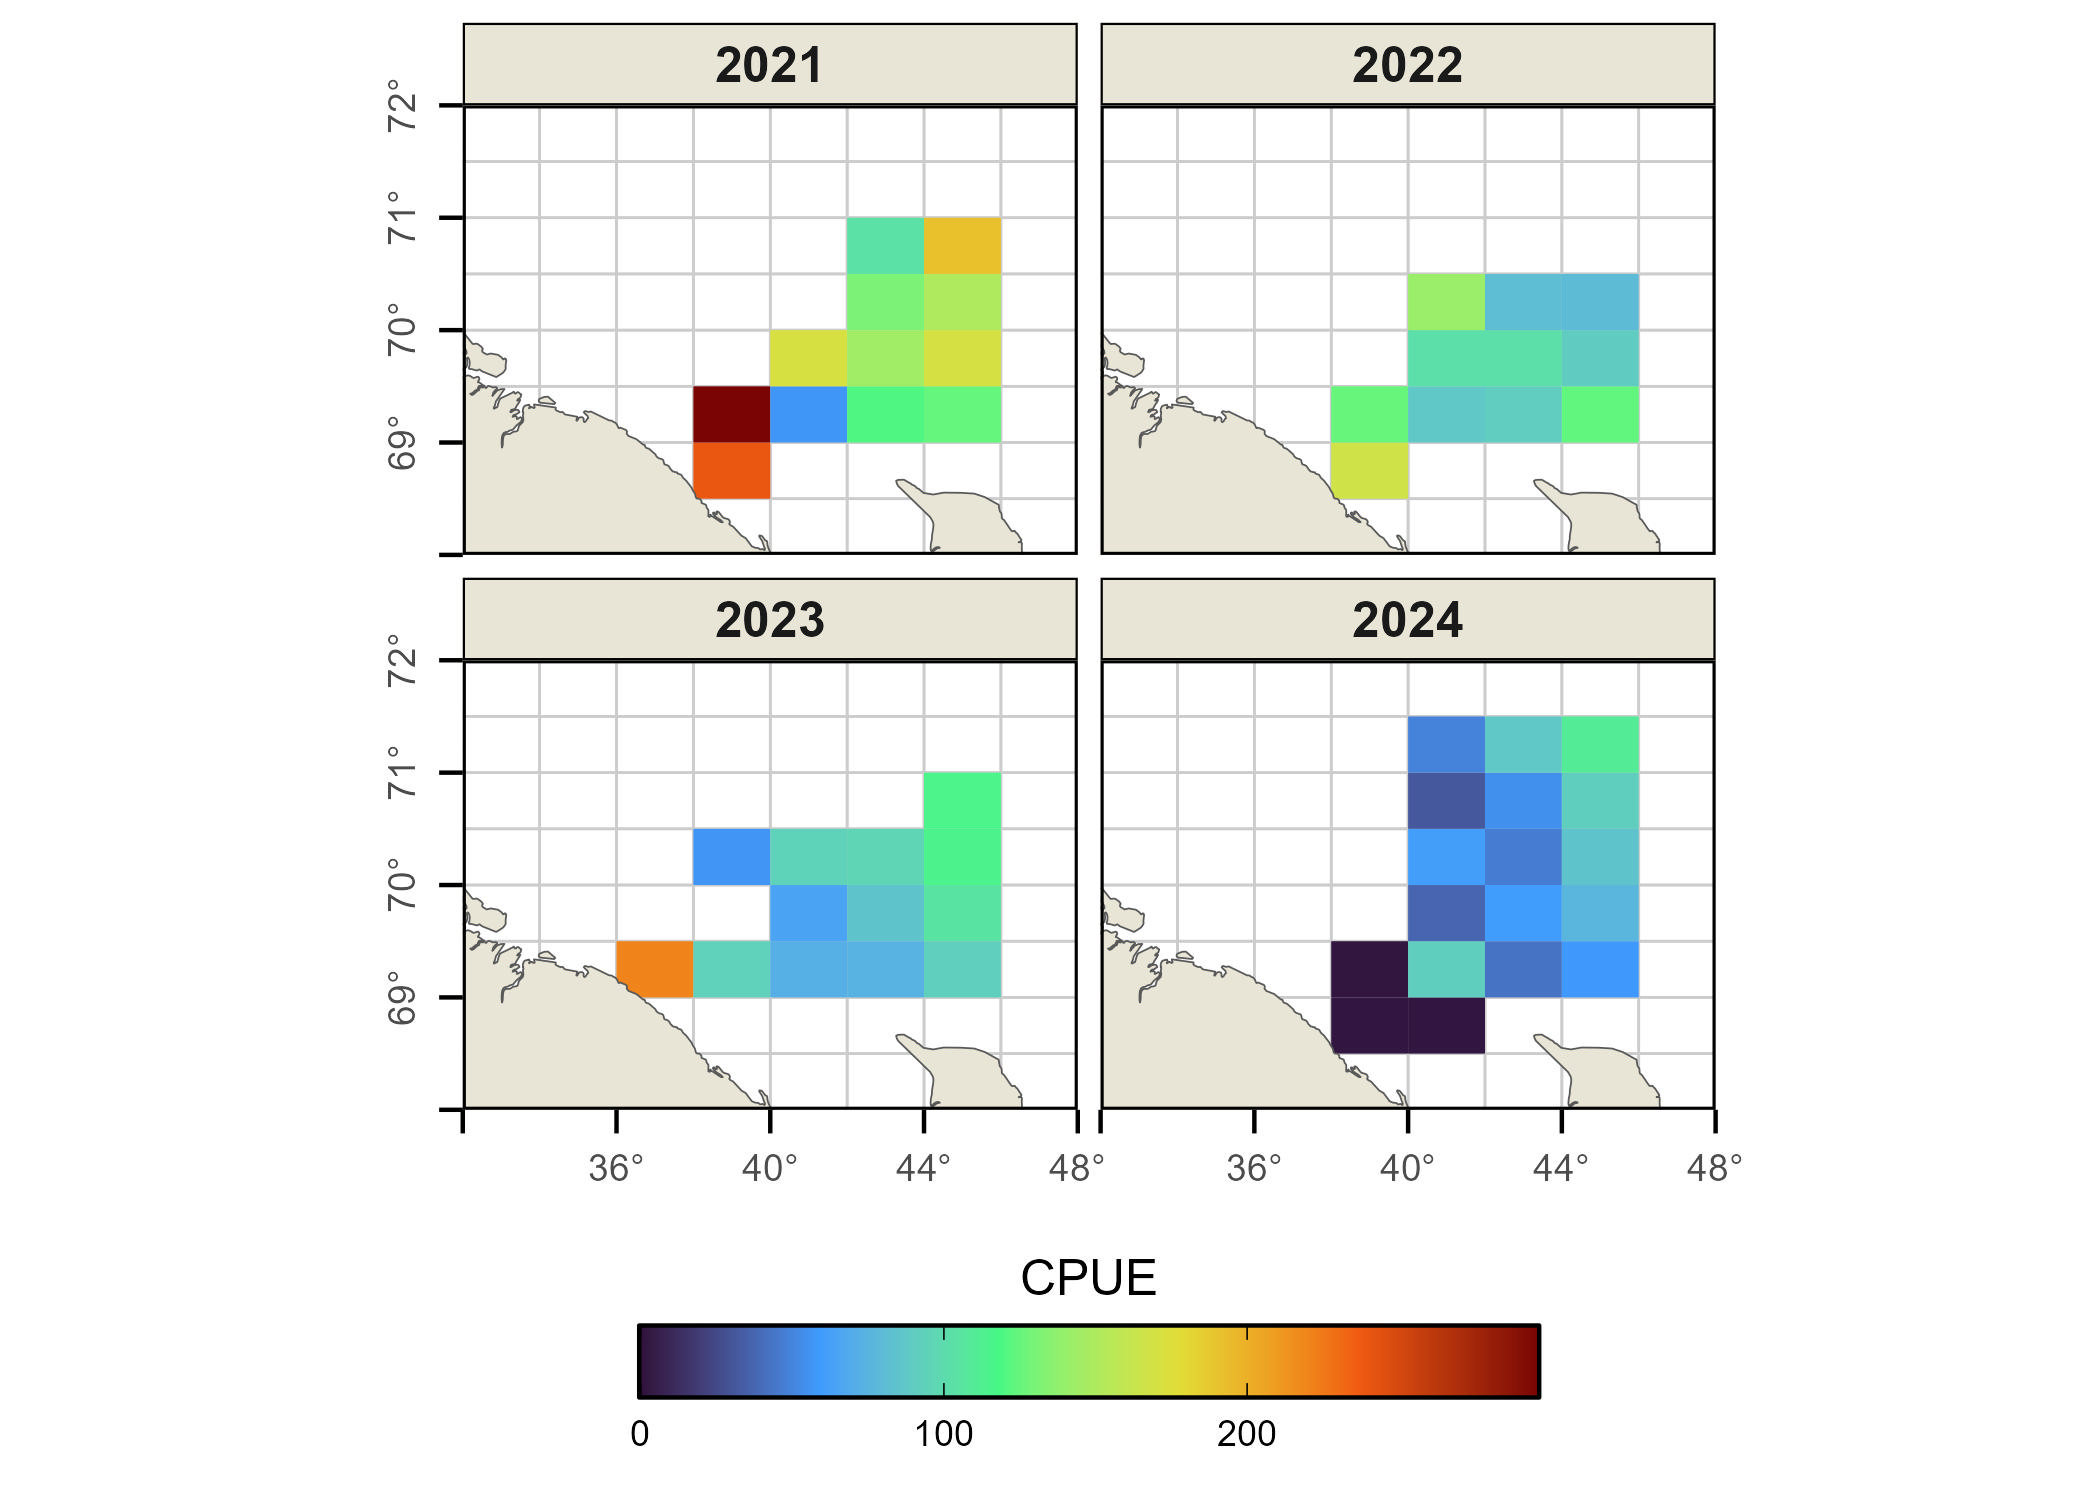
\includegraphics[width=0.8\linewidth,height=\textheight,keepaspectratio]{images/KARTOGRAPH11.PNG}

}

\caption{Рис. 11.: Промысловые карты - картограммы по фасеткам}

\end{figure}%

\begin{Shaded}
\begin{Highlighting}[]
\CommentTok{\# Очистка окружения и установка рабочей директории}
\FunctionTok{rm}\NormalTok{(}\AttributeTok{list =} \FunctionTok{ls}\NormalTok{())}
\FunctionTok{setwd}\NormalTok{(}\StringTok{"C:/COURSES/KARTOGRAPH/"}\NormalTok{)}

\FunctionTok{library}\NormalTok{(rnaturalearth)}
\FunctionTok{library}\NormalTok{(tidyverse)}
\FunctionTok{library}\NormalTok{(ggspatial)}
\FunctionTok{library}\NormalTok{(sf)}

\DocumentationTok{\#\#\#\#\#\#\# READ DATA AND PREPARE SPATIAL OBJECTS \#\#\#\#\#\#\#\#\#\#\#\#\#\#\#\#\#\#\#\#\#\#\#\#\#\#\#\#}

\CommentTok{\# Чтение и фильтрация данных}
\NormalTok{DATA }\OtherTok{\textless{}{-}}\NormalTok{ readxl}\SpecialCharTok{::}\FunctionTok{read\_excel}\NormalTok{(}\StringTok{"KARTOGRAPHIC.xlsx"}\NormalTok{, }\AttributeTok{sheet =} \StringTok{"FISHERY"}\NormalTok{) }\SpecialCharTok{\%\textgreater{}\%} 
  \FunctionTok{filter}\NormalTok{(YEAR }\SpecialCharTok{\textgreater{}} \DecValTok{2020} \SpecialCharTok{\&}\NormalTok{ YEAR }\SpecialCharTok{\textless{}} \DecValTok{2025}\NormalTok{)}

\CommentTok{\# Карта России}
\NormalTok{russia }\OtherTok{\textless{}{-}} \FunctionTok{ne\_countries}\NormalTok{(}\AttributeTok{scale =} \DecValTok{10}\NormalTok{, }\AttributeTok{country =} \StringTok{"Russia"}\NormalTok{) }

\CommentTok{\# Параметры карты и сетки}
\NormalTok{xmin }\OtherTok{\textless{}{-}} \DecValTok{32}\NormalTok{; xmax }\OtherTok{\textless{}{-}} \DecValTok{48}\NormalTok{; ymin }\OtherTok{\textless{}{-}} \DecValTok{68}\NormalTok{; ymax }\OtherTok{\textless{}{-}} \DecValTok{72}
\NormalTok{xcs }\OtherTok{\textless{}{-}} \DecValTok{2}\NormalTok{; ycs }\OtherTok{\textless{}{-}} \FloatTok{0.5}

\CommentTok{\# Преобразование в пространственные объекты}
\NormalTok{points\_sf }\OtherTok{\textless{}{-}} \FunctionTok{st\_as\_sf}\NormalTok{(DATA, }\AttributeTok{coords =} \FunctionTok{c}\NormalTok{(}\StringTok{"X"}\NormalTok{, }\StringTok{"Y"}\NormalTok{), }\AttributeTok{crs =} \DecValTok{4326}\NormalTok{)}

\CommentTok{\# Создание сетки}
\NormalTok{grid\_sf }\OtherTok{\textless{}{-}} \FunctionTok{st\_make\_grid}\NormalTok{(}
\NormalTok{  points\_sf,}
  \AttributeTok{cellsize =} \FunctionTok{c}\NormalTok{(xcs, ycs),}
  \AttributeTok{n =} \FunctionTok{c}\NormalTok{(}\DecValTok{2} \SpecialCharTok{+}\NormalTok{ (xmax }\SpecialCharTok{{-}}\NormalTok{ xmin)}\SpecialCharTok{/}\NormalTok{xcs, }\DecValTok{2} \SpecialCharTok{+}\NormalTok{ (ymax }\SpecialCharTok{{-}}\NormalTok{ ymin)}\SpecialCharTok{/}\NormalTok{ycs),}
  \AttributeTok{offset =} \FunctionTok{c}\NormalTok{(xmin }\SpecialCharTok{{-}}\NormalTok{ xcs, ymin }\SpecialCharTok{{-}}\NormalTok{ ycs)}
\NormalTok{) }\SpecialCharTok{\%\textgreater{}\%} 
  \FunctionTok{st\_sf}\NormalTok{() }\SpecialCharTok{\%\textgreater{}\%} 
  \FunctionTok{mutate}\NormalTok{(}\AttributeTok{cell\_id =} \FunctionTok{row\_number}\NormalTok{())}

\CommentTok{\# Агрегация данных по сетке и годам}
\NormalTok{shares\_df\_catch }\OtherTok{\textless{}{-}}\NormalTok{ points\_sf }\SpecialCharTok{\%\textgreater{}\%} 
  \FunctionTok{st\_join}\NormalTok{(grid\_sf) }\SpecialCharTok{\%\textgreater{}\%} 
  \FunctionTok{st\_drop\_geometry}\NormalTok{() }\SpecialCharTok{\%\textgreater{}\%} 
  \FunctionTok{group\_by}\NormalTok{(cell\_id, YEAR) }\SpecialCharTok{\%\textgreater{}\%} 
  \FunctionTok{summarise}\NormalTok{(}\AttributeTok{CATCH =} \FunctionTok{mean}\NormalTok{(CPUE, }\AttributeTok{na.rm =} \ConstantTok{TRUE}\NormalTok{), }\AttributeTok{.groups =} \StringTok{\textquotesingle{}drop\textquotesingle{}}\NormalTok{)}

\CommentTok{\# Присоединение статистики к сетке}
\NormalTok{gird\_shares\_catch }\OtherTok{\textless{}{-}}\NormalTok{ grid\_sf }\SpecialCharTok{\%\textgreater{}\%} 
  \FunctionTok{right\_join}\NormalTok{(shares\_df\_catch, }\AttributeTok{by =} \StringTok{"cell\_id"}\NormalTok{)}

\DocumentationTok{\#\#\#\#\#\#\#\#\#\#\#\#\#\#\#\#\#\#\#\# ВИЗУАЛИЗАЦИЯ \#\#\#\#\#\#\#\#\#\#\#\#\#\#\#\#\#\#\#\#\#\#\#\#\#\#\#\#\#\#\#\#\#\#\#\#\#\#\#\#\#}

\CommentTok{\# Определяем общий максимум CPUE для единой шкалы цветов}
\NormalTok{catch\_max }\OtherTok{\textless{}{-}} \FunctionTok{max}\NormalTok{(gird\_shares\_catch}\SpecialCharTok{$}\NormalTok{CATCH, }\AttributeTok{na.rm =} \ConstantTok{TRUE}\NormalTok{)}

\FunctionTok{ggplot}\NormalTok{() }\SpecialCharTok{+}
  \CommentTok{\# Контуры сетки}
  \FunctionTok{geom\_sf}\NormalTok{(}\AttributeTok{data =}\NormalTok{ grid\_sf, }\AttributeTok{fill =} \ConstantTok{NA}\NormalTok{, }\AttributeTok{color =} \StringTok{"grey80"}\NormalTok{, }\AttributeTok{linewidth =} \FloatTok{0.3}\NormalTok{) }\SpecialCharTok{+}
  
  \CommentTok{\# Заливка по улову с цветовой схемой viridis}
  \FunctionTok{geom\_sf}\NormalTok{(}\AttributeTok{data =}\NormalTok{ gird\_shares\_catch, }\FunctionTok{aes}\NormalTok{(}\AttributeTok{fill =}\NormalTok{ CATCH), }\AttributeTok{color =} \ConstantTok{NA}\NormalTok{) }\SpecialCharTok{+}
  
  \CommentTok{\# Границы России}
  \FunctionTok{geom\_sf}\NormalTok{(}\AttributeTok{data =}\NormalTok{ russia, }\AttributeTok{fill =} \StringTok{"\#E8E5D6"}\NormalTok{) }\SpecialCharTok{+}
  
  \CommentTok{\# Фасетирование по годам}
  \FunctionTok{facet\_wrap}\NormalTok{(}\SpecialCharTok{\textasciitilde{}}\NormalTok{ YEAR, }\AttributeTok{nrow =} \DecValTok{2}\NormalTok{) }\SpecialCharTok{+}
  
 \CommentTok{\# 4. Цветовая шкала viridis option "H" для заливки}
  \FunctionTok{scale\_fill\_viridis\_c}\NormalTok{(}
    \AttributeTok{option =} \StringTok{"H"}\NormalTok{, }
    \AttributeTok{name =} \StringTok{"CPUE"}\NormalTok{,}
    \AttributeTok{limits =} \FunctionTok{c}\NormalTok{(}\DecValTok{0}\NormalTok{, }\FunctionTok{max}\NormalTok{(gird\_shares\_catch}\SpecialCharTok{$}\NormalTok{CATCH, }\AttributeTok{na.rm =} \ConstantTok{TRUE}\NormalTok{)),}
    \AttributeTok{na.value =} \StringTok{"transparent"}
\NormalTok{  ) }\SpecialCharTok{+}

 
  \CommentTok{\# Область отображения}
  \FunctionTok{coord\_sf}\NormalTok{(}
    \AttributeTok{xlim =} \FunctionTok{c}\NormalTok{(xmin, xmax), }
    \AttributeTok{ylim =} \FunctionTok{c}\NormalTok{(ymin, ymax),}
    \AttributeTok{expand =} \ConstantTok{FALSE}
\NormalTok{  ) }\SpecialCharTok{+}

  
  \CommentTok{\# Оформление}
  \FunctionTok{theme\_minimal}\NormalTok{() }\SpecialCharTok{+}
  \FunctionTok{theme}\NormalTok{(}
    \AttributeTok{panel.grid =} \FunctionTok{element\_blank}\NormalTok{(),}
    \AttributeTok{legend.position =} \StringTok{"bottom"}\NormalTok{,}
    \AttributeTok{legend.key.width =} \FunctionTok{unit}\NormalTok{(}\FloatTok{2.5}\NormalTok{, }\StringTok{"cm"}\NormalTok{),}
    \AttributeTok{legend.title =} \FunctionTok{element\_text}\NormalTok{(}\AttributeTok{vjust =} \FloatTok{0.8}\NormalTok{, }\AttributeTok{size =} \DecValTok{12}\NormalTok{),}
    \AttributeTok{panel.border =} \FunctionTok{element\_rect}\NormalTok{(}\AttributeTok{fill =} \ConstantTok{NA}\NormalTok{, }\AttributeTok{color =} \StringTok{"black"}\NormalTok{, }\AttributeTok{size =} \FloatTok{0.7}\NormalTok{),}
    \AttributeTok{panel.grid.major =} \FunctionTok{element\_line}\NormalTok{(}\AttributeTok{color =} \StringTok{"grey90"}\NormalTok{, }\AttributeTok{size =} \FloatTok{0.2}\NormalTok{),}
    \AttributeTok{strip.background =} \FunctionTok{element\_rect}\NormalTok{(}\AttributeTok{fill =} \StringTok{"\#E8E5D6"}\NormalTok{, }\AttributeTok{color =} \StringTok{"black"}\NormalTok{),}
    \AttributeTok{strip.text =} \FunctionTok{element\_text}\NormalTok{(}\AttributeTok{face =} \StringTok{"bold"}\NormalTok{, }\AttributeTok{size =} \DecValTok{12}\NormalTok{)}
\NormalTok{  ) }\SpecialCharTok{+}
  
  \CommentTok{\# Настройка легенды}
  \FunctionTok{guides}\NormalTok{(}\AttributeTok{fill =} \FunctionTok{guide\_colorbar}\NormalTok{(}
    \AttributeTok{title.position =} \StringTok{"top"}\NormalTok{,}
    \AttributeTok{title.hjust =} \FloatTok{0.5}\NormalTok{,}
    \AttributeTok{barwidth =} \DecValTok{15}\NormalTok{,}
    \AttributeTok{frame.colour =} \StringTok{"black"}\NormalTok{,}
    \AttributeTok{ticks.colour =} \StringTok{"black"}
\NormalTok{  ))}
\NormalTok{    na.value }\OtherTok{=} \ConstantTok{NA}\NormalTok{,}
\NormalTok{    limits }\OtherTok{=} \FunctionTok{c}\NormalTok{(}\DecValTok{0}\NormalTok{, }\FunctionTok{max}\NormalTok{(gird\_shares\_catch}\SpecialCharTok{$}\NormalTok{CATCH, }\AttributeTok{na.rm =} \ConstantTok{TRUE}\NormalTok{))}
  \ErrorTok{)} \SpecialCharTok{+}

  
  \CommentTok{\# Область отображения}
  \FunctionTok{coord\_sf}\NormalTok{(}\AttributeTok{xlim =} \FunctionTok{c}\NormalTok{(xmin, xmax), }\AttributeTok{ylim =} \FunctionTok{c}\NormalTok{(ymin, ymax)) }\SpecialCharTok{+}
  
  \CommentTok{\# Оформление}
  \FunctionTok{theme\_minimal}\NormalTok{() }\SpecialCharTok{+}
  \FunctionTok{theme}\NormalTok{(}
    \AttributeTok{axis.text.x =} \FunctionTok{element\_text}\NormalTok{(}\AttributeTok{size =} \DecValTok{8}\NormalTok{),}
    \AttributeTok{axis.text.y =} \FunctionTok{element\_text}\NormalTok{(}\AttributeTok{size =} \DecValTok{8}\NormalTok{, }\AttributeTok{angle =} \DecValTok{90}\NormalTok{, }\AttributeTok{hjust =} \FloatTok{0.5}\NormalTok{),}
    \AttributeTok{panel.grid =} \FunctionTok{element\_line}\NormalTok{(}\AttributeTok{color =} \StringTok{"grey90"}\NormalTok{),}
    \AttributeTok{legend.position =} \StringTok{"bottom"}\NormalTok{,}
    \AttributeTok{panel.border =} \FunctionTok{element\_rect}\NormalTok{(}\AttributeTok{fill =} \ConstantTok{NA}\NormalTok{, }\AttributeTok{color =} \StringTok{"black"}\NormalTok{, }\AttributeTok{size =} \FloatTok{0.5}\NormalTok{),}
    \AttributeTok{strip.background =} \FunctionTok{element\_rect}\NormalTok{(}\AttributeTok{fill =} \StringTok{"white"}\NormalTok{, }\AttributeTok{color =} \StringTok{"black"}\NormalTok{)}
\NormalTok{  ) }\SpecialCharTok{+}
  \FunctionTok{guides}\NormalTok{(}\AttributeTok{fill =} \FunctionTok{guide\_colorbar}\NormalTok{(}\AttributeTok{title =} \ConstantTok{NULL}\NormalTok{))}
\end{Highlighting}
\end{Shaded}

\section{Гибридные карты - картограммы и точки (съемка и промысловые
данные)}\label{ux433ux438ux431ux440ux438ux434ux43dux44bux435-ux43aux430ux440ux442ux44b---ux43aux430ux440ux442ux43eux433ux440ux430ux43cux43cux44b-ux438-ux442ux43eux447ux43aux438-ux441ux44aux435ux43cux43aux430-ux438-ux43fux440ux43eux43cux44bux441ux43bux43eux432ux44bux435-ux434ux430ux43dux43dux44bux435}

\begin{figure}[H]

{\centering 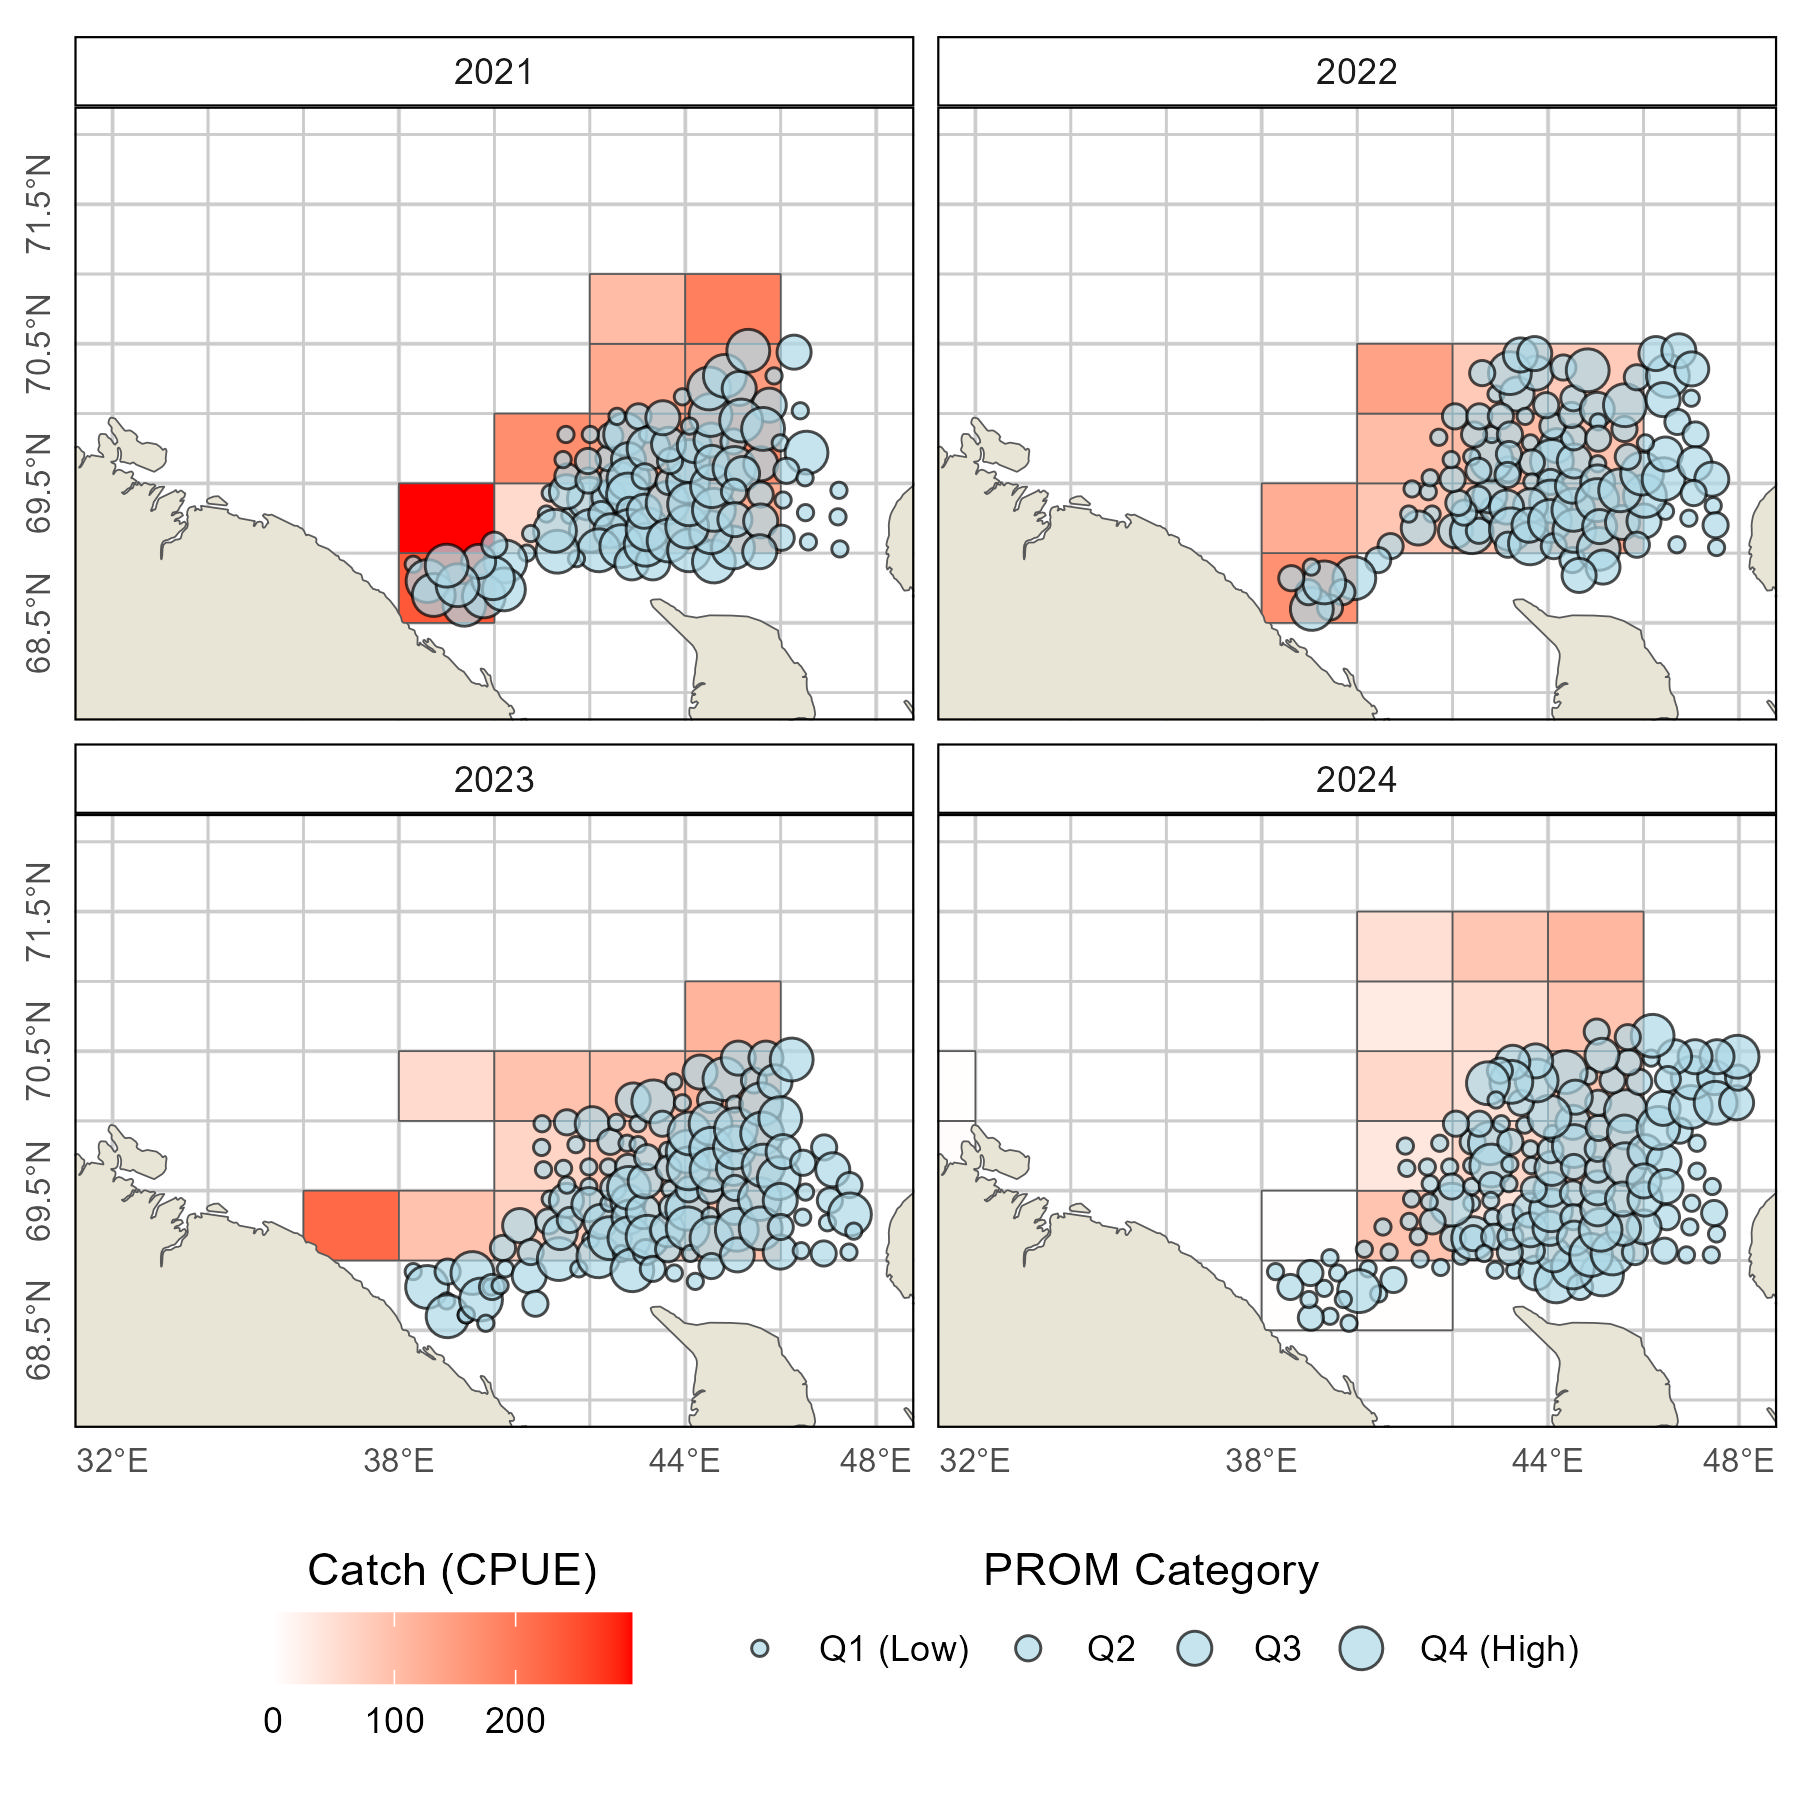
\includegraphics[width=0.8\linewidth,height=\textheight,keepaspectratio]{images/KARTOGRAPH12.PNG}

}

\caption{Рис. 12.: Гибридные карты - картограммы и точки (съемка и
промысловые данные)}

\end{figure}%

\begin{Shaded}
\begin{Highlighting}[]
\CommentTok{\# Очистка окружения и установка рабочей директории}
\FunctionTok{rm}\NormalTok{(}\AttributeTok{list =} \FunctionTok{ls}\NormalTok{())}
\FunctionTok{setwd}\NormalTok{(}\StringTok{"C:/COURSES/KARTOGRAPH/"}\NormalTok{)}

\FunctionTok{library}\NormalTok{(rnaturalearth)}
\FunctionTok{library}\NormalTok{(tidyverse)}
\FunctionTok{library}\NormalTok{(ggspatial)}
\FunctionTok{library}\NormalTok{(sf)}

\DocumentationTok{\#\#\#\#\#\#\# READ DATA AND PREPARE SPATIAL OBJECTS \#\#\#\#\#\#\#\#\#\#\#\#\#\#\#\#\#\#\#\#\#\#\#\#\#\#\#\#}

\CommentTok{\# Чтение и фильтрация данных}
\NormalTok{DATA }\OtherTok{\textless{}{-}}\NormalTok{ readxl}\SpecialCharTok{::}\FunctionTok{read\_excel}\NormalTok{(}\StringTok{"KARTOGRAPHIC.xlsx"}\NormalTok{, }\AttributeTok{sheet =} \StringTok{"FISHERY"}\NormalTok{) }\SpecialCharTok{\%\textgreater{}\%} 
  \FunctionTok{filter}\NormalTok{(YEAR }\SpecialCharTok{\textgreater{}} \DecValTok{2020} \SpecialCharTok{\&}\NormalTok{ YEAR }\SpecialCharTok{\textless{}} \DecValTok{2025}\NormalTok{)}

\NormalTok{SURVEY }\OtherTok{\textless{}{-}}\NormalTok{ readxl}\SpecialCharTok{::}\FunctionTok{read\_excel}\NormalTok{(}\StringTok{"KARTOGRAPHIC.xlsx"}\NormalTok{, }\AttributeTok{sheet =} \StringTok{"SURVEY"}\NormalTok{) }\SpecialCharTok{\%\textgreater{}\%} 
  \FunctionTok{filter}\NormalTok{(YEAR }\SpecialCharTok{\textgreater{}} \DecValTok{2020} \SpecialCharTok{\&}\NormalTok{ YEAR }\SpecialCharTok{\textless{}} \DecValTok{2025}\NormalTok{, SURV }\SpecialCharTok{==} \StringTok{"CRAB"}\NormalTok{)}

\CommentTok{\# Создание 4 категорий для переменной PROM}
\NormalTok{breaks }\OtherTok{\textless{}{-}} \FunctionTok{quantile}\NormalTok{(SURVEY}\SpecialCharTok{$}\NormalTok{PROM, }
                   \AttributeTok{probs =} \FunctionTok{c}\NormalTok{(}\DecValTok{0}\NormalTok{, }\FloatTok{0.25}\NormalTok{, }\FloatTok{0.5}\NormalTok{, }\FloatTok{0.75}\NormalTok{, }\DecValTok{1}\NormalTok{), }
                   \AttributeTok{na.rm =} \ConstantTok{TRUE}\NormalTok{)}
\NormalTok{SURVEY}\SpecialCharTok{$}\NormalTok{PROM\_cat }\OtherTok{\textless{}{-}} \FunctionTok{cut}\NormalTok{(SURVEY}\SpecialCharTok{$}\NormalTok{PROM,}
                       \AttributeTok{breaks =}\NormalTok{ breaks,}
                       \AttributeTok{include.lowest =} \ConstantTok{TRUE}\NormalTok{,}
                       \AttributeTok{labels =} \FunctionTok{c}\NormalTok{(}\StringTok{"Q1 (Low)"}\NormalTok{, }\StringTok{"Q2"}\NormalTok{, }\StringTok{"Q3"}\NormalTok{, }\StringTok{"Q4 (High)"}\NormalTok{))}

\CommentTok{\# Карта России}
\NormalTok{russia }\OtherTok{\textless{}{-}} \FunctionTok{ne\_countries}\NormalTok{(}\AttributeTok{scale =} \DecValTok{10}\NormalTok{, }\AttributeTok{country =} \StringTok{"Russia"}\NormalTok{) }

\CommentTok{\# Параметры карты и сетки}
\NormalTok{xmin }\OtherTok{\textless{}{-}} \DecValTok{32}\NormalTok{; xmax }\OtherTok{\textless{}{-}} \DecValTok{48}\NormalTok{; ymin }\OtherTok{\textless{}{-}} \DecValTok{68}\NormalTok{; ymax }\OtherTok{\textless{}{-}} \DecValTok{72}
\NormalTok{xcs }\OtherTok{\textless{}{-}} \DecValTok{2}\NormalTok{; ycs }\OtherTok{\textless{}{-}} \FloatTok{0.5}

\CommentTok{\# Преобразование в пространственные объекты}
\NormalTok{points\_sf }\OtherTok{\textless{}{-}} \FunctionTok{st\_as\_sf}\NormalTok{(DATA, }\AttributeTok{coords =} \FunctionTok{c}\NormalTok{(}\StringTok{"X"}\NormalTok{, }\StringTok{"Y"}\NormalTok{), }\AttributeTok{crs =} \DecValTok{4326}\NormalTok{)}
\NormalTok{survey\_sf }\OtherTok{\textless{}{-}} \FunctionTok{st\_as\_sf}\NormalTok{(SURVEY, }\AttributeTok{coords =} \FunctionTok{c}\NormalTok{(}\StringTok{"X"}\NormalTok{, }\StringTok{"Y"}\NormalTok{), }\AttributeTok{crs =} \DecValTok{4326}\NormalTok{)}

\CommentTok{\# Создание сетки}
\NormalTok{grid\_sf }\OtherTok{\textless{}{-}} \FunctionTok{st\_make\_grid}\NormalTok{(}
\NormalTok{  points\_sf,}
  \AttributeTok{cellsize =} \FunctionTok{c}\NormalTok{(xcs, ycs),}
  \AttributeTok{n =} \FunctionTok{c}\NormalTok{(}\DecValTok{2} \SpecialCharTok{+}\NormalTok{ (xmax }\SpecialCharTok{{-}}\NormalTok{ xmin)}\SpecialCharTok{/}\NormalTok{xcs, }\DecValTok{2} \SpecialCharTok{+}\NormalTok{ (ymax }\SpecialCharTok{{-}}\NormalTok{ ymin)}\SpecialCharTok{/}\NormalTok{ycs),}
  \AttributeTok{offset =} \FunctionTok{c}\NormalTok{(xmin }\SpecialCharTok{{-}}\NormalTok{ xcs, ymin }\SpecialCharTok{{-}}\NormalTok{ ycs)}
\NormalTok{) }\SpecialCharTok{\%\textgreater{}\%} 
  \FunctionTok{st\_sf}\NormalTok{() }\SpecialCharTok{\%\textgreater{}\%} 
  \FunctionTok{mutate}\NormalTok{(}\AttributeTok{cell\_id =} \FunctionTok{row\_number}\NormalTok{())}

\CommentTok{\# Агрегация данных по сетке и годам}
\NormalTok{shares\_df\_catch }\OtherTok{\textless{}{-}}\NormalTok{ points\_sf }\SpecialCharTok{\%\textgreater{}\%} 
  \FunctionTok{st\_join}\NormalTok{(grid\_sf) }\SpecialCharTok{\%\textgreater{}\%} 
  \FunctionTok{st\_drop\_geometry}\NormalTok{() }\SpecialCharTok{\%\textgreater{}\%} 
  \FunctionTok{group\_by}\NormalTok{(cell\_id, YEAR) }\SpecialCharTok{\%\textgreater{}\%} 
  \FunctionTok{summarise}\NormalTok{(}\AttributeTok{CATCH =} \FunctionTok{mean}\NormalTok{(CPUE, }\AttributeTok{na.rm =} \ConstantTok{TRUE}\NormalTok{), }\AttributeTok{.groups =} \StringTok{\textquotesingle{}drop\textquotesingle{}}\NormalTok{)}

\CommentTok{\# Присоединение статистики к сетке}
\NormalTok{gird\_shares\_catch }\OtherTok{\textless{}{-}}\NormalTok{ grid\_sf }\SpecialCharTok{\%\textgreater{}\%} 
  \FunctionTok{right\_join}\NormalTok{(shares\_df\_catch, }\AttributeTok{by =} \StringTok{"cell\_id"}\NormalTok{)}

\DocumentationTok{\#\#\#\#\#\#\#\#\#\#\#\#\#\#\#\#\#\#\# ВИЗУАЛИЗАЦИЯ \#\#\#\#\#\#\#\#\#\#\#\#\#\#\#\#\#\#\#\#\#\#\#\#\#\#\#\#\#\#\#\#\#\#\#\#\#\#\#\#\#}
\FunctionTok{ggplot}\NormalTok{() }\SpecialCharTok{+}
  \CommentTok{\# Контуры сетки}
  \FunctionTok{geom\_sf}\NormalTok{(}\AttributeTok{data =}\NormalTok{ grid\_sf, }\AttributeTok{fill =} \ConstantTok{NA}\NormalTok{, }\AttributeTok{color =} \StringTok{"grey80"}\NormalTok{, }\AttributeTok{linewidth =} \FloatTok{0.3}\NormalTok{) }\SpecialCharTok{+}
  
  \CommentTok{\# Заливка по улову (средний CPUE)}
  \FunctionTok{geom\_sf}\NormalTok{(}\AttributeTok{data =}\NormalTok{ gird\_shares\_catch, }\FunctionTok{aes}\NormalTok{(}\AttributeTok{fill =}\NormalTok{ CATCH)) }\SpecialCharTok{+}
  
  \CommentTok{\# Границы России}
  \FunctionTok{geom\_sf}\NormalTok{(}\AttributeTok{data =}\NormalTok{ russia, }\AttributeTok{fill =} \StringTok{"\#E8E5D6"}\NormalTok{) }\SpecialCharTok{+}
  
  \CommentTok{\# Точки SURVEY: голубые с черной окантовкой}
  \FunctionTok{geom\_sf}\NormalTok{(}\AttributeTok{data =}\NormalTok{ survey\_sf, }
          \FunctionTok{aes}\NormalTok{(}\AttributeTok{size =}\NormalTok{ PROM\_cat),}
          \AttributeTok{fill =} \StringTok{"lightblue"}\NormalTok{,    }\CommentTok{\# Голубая заливка}
          \AttributeTok{color =} \StringTok{"black"}\NormalTok{,        }\CommentTok{\# Черная окантовка}
          \AttributeTok{alpha =} \FloatTok{0.7}\NormalTok{,}
          \AttributeTok{shape =} \DecValTok{21}\NormalTok{,             }\CommentTok{\# Круг с обводкой}
          \AttributeTok{stroke =} \FloatTok{0.5}\NormalTok{,           }\CommentTok{\# Толщина окантовки}
          \AttributeTok{show.legend =} \StringTok{"point"}\NormalTok{) }\SpecialCharTok{+}
  
  \CommentTok{\# Фасетирование по годам}
  \FunctionTok{facet\_wrap}\NormalTok{(}\SpecialCharTok{\textasciitilde{}}\NormalTok{ YEAR, }\AttributeTok{nrow =} \DecValTok{2}\NormalTok{) }\SpecialCharTok{+}
  
  \CommentTok{\# Цветовая шкала для заливки}
  \FunctionTok{scale\_fill\_gradient}\NormalTok{(}
    \AttributeTok{low =} \StringTok{"white"}\NormalTok{, }
    \AttributeTok{high =} \StringTok{"red"}\NormalTok{,}
    \AttributeTok{na.value =} \ConstantTok{NA}\NormalTok{,}
    \AttributeTok{limits =} \FunctionTok{c}\NormalTok{(}\DecValTok{0}\NormalTok{, }\FunctionTok{max}\NormalTok{(gird\_shares\_catch}\SpecialCharTok{$}\NormalTok{CATCH, }\AttributeTok{na.rm =} \ConstantTok{TRUE}\NormalTok{)),}
    \AttributeTok{name =} \StringTok{"Catch (CPUE)"}
\NormalTok{  ) }\SpecialCharTok{+}
  
  \CommentTok{\# Шкала размеров для точек}
  \FunctionTok{scale\_size\_manual}\NormalTok{(}
    \AttributeTok{name =} \StringTok{"PROM Category"}\NormalTok{,}
    \AttributeTok{values =} \FunctionTok{c}\NormalTok{(}\FloatTok{1.5}\NormalTok{, }\FloatTok{2.5}\NormalTok{, }\FloatTok{3.5}\NormalTok{, }\FloatTok{4.5}\NormalTok{)  }\CommentTok{\# Размеры точек для 4 категорий}
\NormalTok{  ) }\SpecialCharTok{+}
  
  \DocumentationTok{\#\#\# ОСИ С ГЕОГРАФИЧЕСКИМИ КООРДИНАТАМИ }\AlertTok{\#\#\#}
  \FunctionTok{scale\_x\_continuous}\NormalTok{(}
    \AttributeTok{breaks =} \FunctionTok{c}\NormalTok{(}\DecValTok{32}\NormalTok{, }\DecValTok{38}\NormalTok{, }\DecValTok{44}\NormalTok{, }\DecValTok{48}\NormalTok{),                    }
    \AttributeTok{labels =} \FunctionTok{c}\NormalTok{(}\StringTok{"32°E"}\NormalTok{, }\StringTok{"38°E"}\NormalTok{, }\StringTok{"44°E"}\NormalTok{, }\StringTok{"48°E"}\NormalTok{),    }
    \AttributeTok{name =} \ConstantTok{NULL}
\NormalTok{  ) }\SpecialCharTok{+}
  \FunctionTok{scale\_y\_continuous}\NormalTok{(}
    \AttributeTok{breaks =} \FunctionTok{c}\NormalTok{(}\FloatTok{68.5}\NormalTok{, }\FloatTok{69.5}\NormalTok{, }\FloatTok{70.5}\NormalTok{, }\FloatTok{71.5}\NormalTok{),          }
    \AttributeTok{labels =} \FunctionTok{c}\NormalTok{(}\StringTok{"68.5°N"}\NormalTok{, }\StringTok{"69.5°N"}\NormalTok{, }\StringTok{"70.5°N"}\NormalTok{, }\StringTok{"71.5°N"}\NormalTok{),}
    \AttributeTok{name =} \ConstantTok{NULL}
\NormalTok{  ) }\SpecialCharTok{+}
  
  \CommentTok{\# Область отображения}
  \FunctionTok{coord\_sf}\NormalTok{(}\AttributeTok{xlim =} \FunctionTok{c}\NormalTok{(xmin, xmax), }\AttributeTok{ylim =} \FunctionTok{c}\NormalTok{(ymin, ymax)) }\SpecialCharTok{+}
  
  \CommentTok{\# Оформление}
  \FunctionTok{theme\_minimal}\NormalTok{() }\SpecialCharTok{+}
  \FunctionTok{theme}\NormalTok{(}
    \AttributeTok{axis.text.x =} \FunctionTok{element\_text}\NormalTok{(}\AttributeTok{size =} \DecValTok{8}\NormalTok{),}
    \AttributeTok{axis.text.y =} \FunctionTok{element\_text}\NormalTok{(}\AttributeTok{size =} \DecValTok{8}\NormalTok{, }\AttributeTok{angle =} \DecValTok{90}\NormalTok{, }\AttributeTok{hjust =} \FloatTok{0.5}\NormalTok{),}
    \AttributeTok{panel.grid =} \FunctionTok{element\_line}\NormalTok{(}\AttributeTok{color =} \StringTok{"grey90"}\NormalTok{),}
    \AttributeTok{legend.position =} \StringTok{"bottom"}\NormalTok{,}
    \AttributeTok{legend.box =} \StringTok{"horizontal"}\NormalTok{,  }\CommentTok{\# Размещение легенд в одну строку}
    \AttributeTok{panel.border =} \FunctionTok{element\_rect}\NormalTok{(}\AttributeTok{fill =} \ConstantTok{NA}\NormalTok{, }\AttributeTok{color =} \StringTok{"black"}\NormalTok{, }\AttributeTok{size =} \FloatTok{0.5}\NormalTok{),}
    \AttributeTok{strip.background =} \FunctionTok{element\_rect}\NormalTok{(}\AttributeTok{fill =} \StringTok{"white"}\NormalTok{, }\AttributeTok{color =} \StringTok{"black"}\NormalTok{)}
\NormalTok{  ) }\SpecialCharTok{+}
  \CommentTok{\# Управление легендами}
  \FunctionTok{guides}\NormalTok{(}
    \AttributeTok{fill =} \FunctionTok{guide\_colorbar}\NormalTok{(}\AttributeTok{title.position =} \StringTok{"top"}\NormalTok{, }\AttributeTok{title.hjust =} \FloatTok{0.5}\NormalTok{),}
    \AttributeTok{size =} \FunctionTok{guide\_legend}\NormalTok{(}\AttributeTok{title.position =} \StringTok{"top"}\NormalTok{, }\AttributeTok{title.hjust =} \FloatTok{0.5}\NormalTok{)}
\NormalTok{  )}
\end{Highlighting}
\end{Shaded}

\section{Карты для ``главы Материал и
методы''}\label{ux43aux430ux440ux442ux44b-ux434ux43bux44f-ux433ux43bux430ux432ux44b-ux43cux430ux442ux435ux440ux438ux430ux43b-ux438-ux43cux435ux442ux43eux434ux44b}

\begin{figure}[H]

{\centering 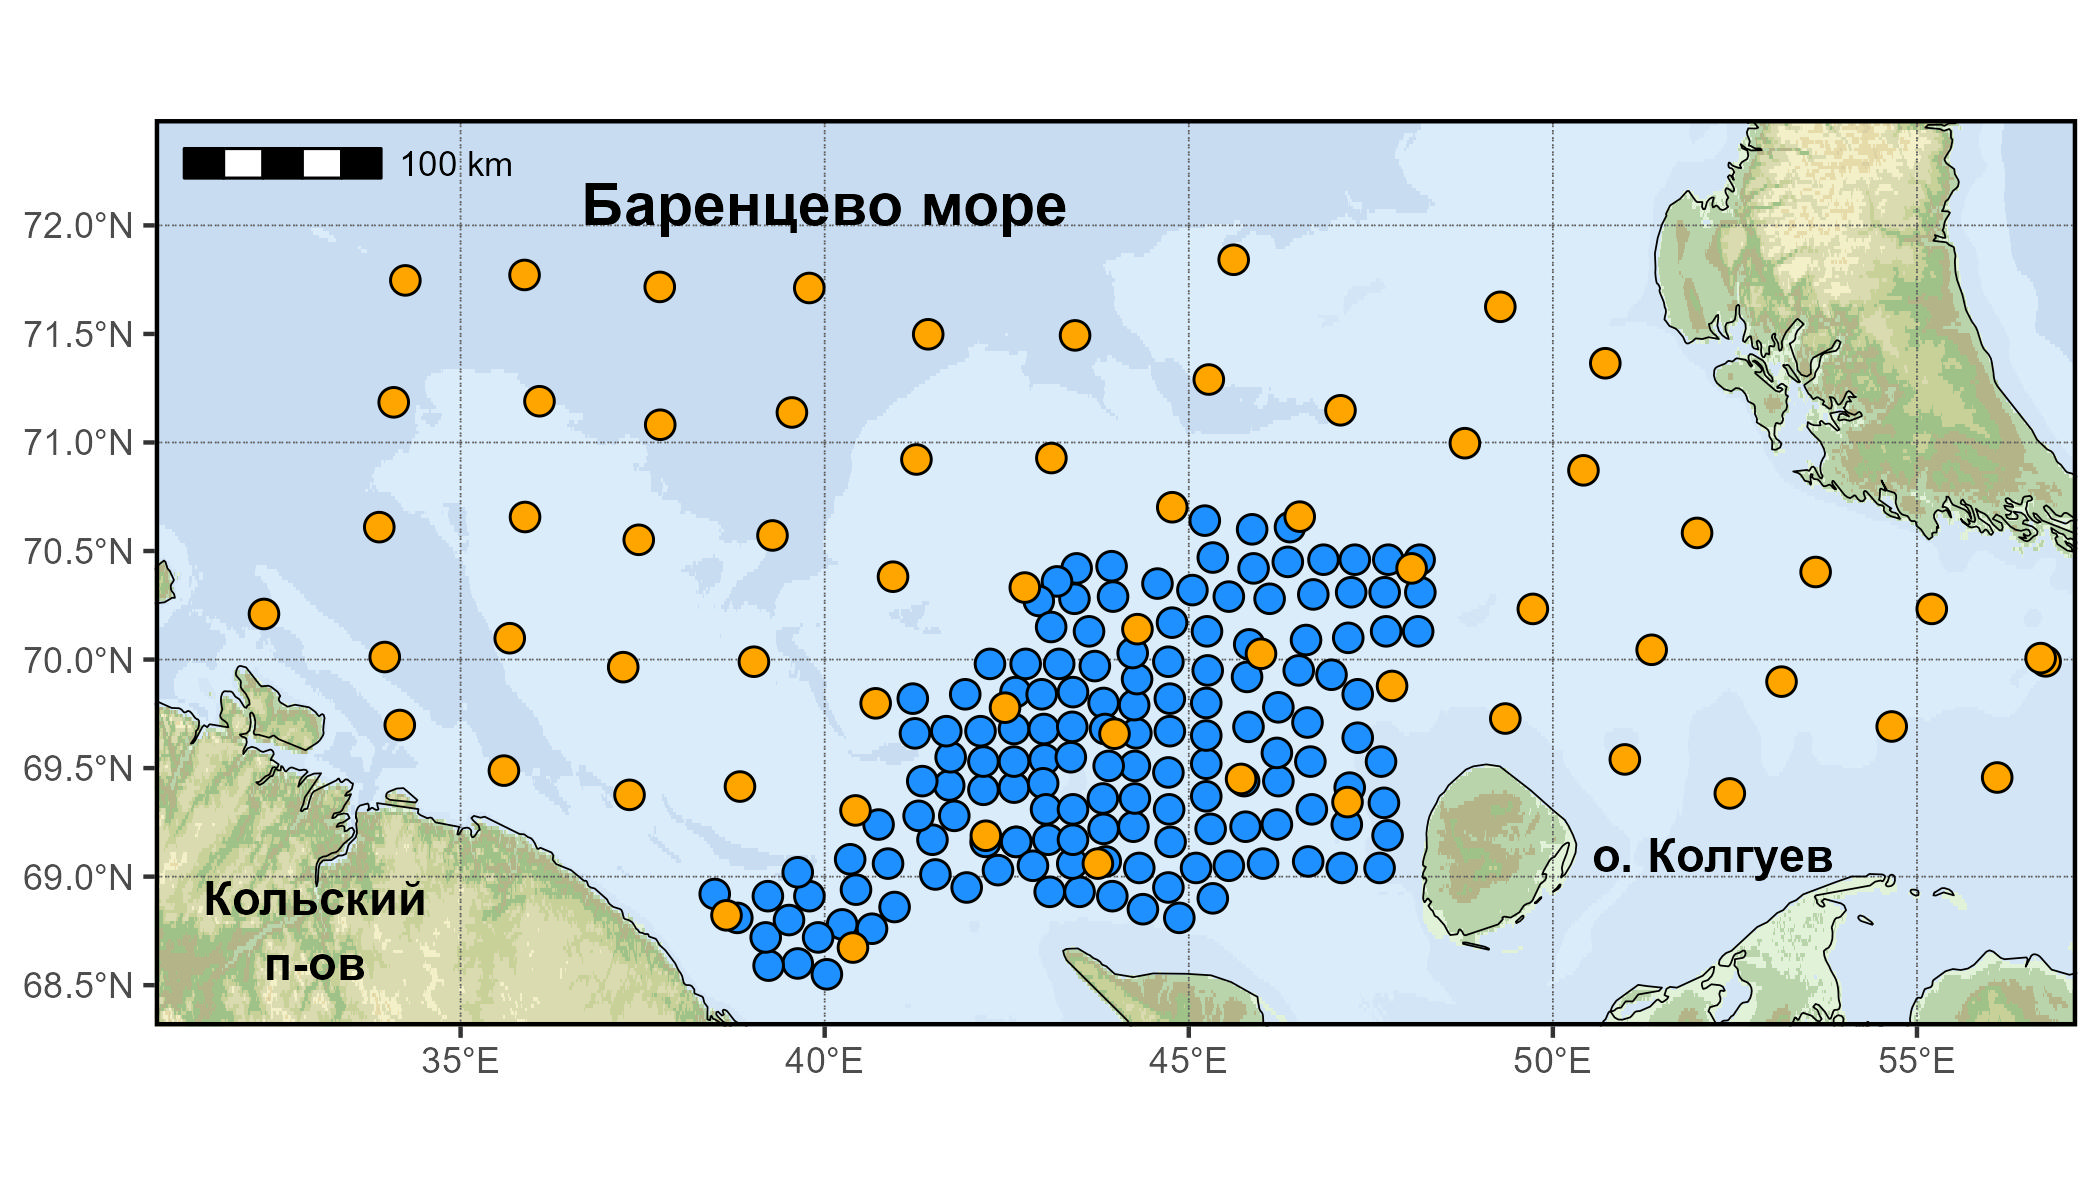
\includegraphics[width=0.8\linewidth,height=\textheight,keepaspectratio]{images/KARTOGRAPH13.PNG}

}

\caption{Рис. 13.: Карты для ``главы Материал и методы''}

\end{figure}%

\begin{Shaded}
\begin{Highlighting}[]
\CommentTok{\# Очистка окружения и установка рабочей директории}
\FunctionTok{rm}\NormalTok{(}\AttributeTok{list =} \FunctionTok{ls}\NormalTok{()) }\CommentTok{\# Удаление всех объектов из глобального окружения}
\FunctionTok{setwd}\NormalTok{(}\StringTok{"C:/COURSES/KARTOGRAPH/"}\NormalTok{) }\CommentTok{\# Установка рабочей директории}

\CommentTok{\# {-}{-}{-}{-}{-}{-}{-}{-}{-}{-}{-}{-}{-}{-}{-}{-}{-}}
\CommentTok{\# ЗАГРУЗКА ПАКЕТОВ}
\CommentTok{\# {-}{-}{-}{-}{-}{-}{-}{-}{-}{-}{-}{-}{-}{-}{-}{-}{-}}
\FunctionTok{library}\NormalTok{(sf)          }\CommentTok{\# Пространственные операции с векторными данными}
\FunctionTok{library}\NormalTok{(marmap)      }\CommentTok{\# Работа с батиметрическими данными (карты глубин)}
\FunctionTok{library}\NormalTok{(tidyverse)   }\CommentTok{\# Коллекция пакетов для обработки данных (dplyr, ggplot2 и др.)}
\FunctionTok{library}\NormalTok{(rnaturalearth) }\CommentTok{\# Векторные картографические данные (границы, береговые линии)}
\FunctionTok{library}\NormalTok{(ggspatial)   }\CommentTok{\# Инструменты для пространственной визуализации в ggplot}
\FunctionTok{library}\NormalTok{(readxl)      }\CommentTok{\# Импорт данных из Excel{-}файлов}

\CommentTok{\# {-}{-}{-}{-}{-}{-}{-}{-}{-}{-}{-}{-}{-}{-}{-}{-}{-}}
\CommentTok{\# ЗАГРУЗКА ДАННЫХ}
\CommentTok{\# {-}{-}{-}{-}{-}{-}{-}{-}{-}{-}{-}{-}{-}{-}{-}{-}{-}}
\CommentTok{\# Чтение данных из Excel{-}листа}
\NormalTok{DATA }\OtherTok{\textless{}{-}}\NormalTok{ readxl}\SpecialCharTok{::}\FunctionTok{read\_excel}\NormalTok{(}\StringTok{"KARTOGRAPHIC.xlsx"}\NormalTok{, }\AttributeTok{sheet =} \StringTok{"SURVEY"}\NormalTok{)}

\CommentTok{\# Фильтрация данных:}
\NormalTok{SUMMER }\OtherTok{\textless{}{-}}\NormalTok{ DATA[DATA}\SpecialCharTok{$}\NormalTok{SURV }\SpecialCharTok{==} \StringTok{"SUM"} \SpecialCharTok{\&}\NormalTok{ DATA}\SpecialCharTok{$}\NormalTok{YEAR }\SpecialCharTok{==} \DecValTok{2024}\NormalTok{, ] }\CommentTok{\# Летние исследования 2024}
\NormalTok{CRAB }\OtherTok{\textless{}{-}}\NormalTok{ DATA[DATA}\SpecialCharTok{$}\NormalTok{SURV }\SpecialCharTok{==} \StringTok{"CRAB"} \SpecialCharTok{\&}\NormalTok{ DATA}\SpecialCharTok{$}\NormalTok{YEAR }\SpecialCharTok{==} \DecValTok{2024}\NormalTok{, ]   }\CommentTok{\# Крабовые исследования 2024}

\CommentTok{\# {-}{-}{-}{-}{-}{-}{-}{-}{-}{-}{-}{-}{-}{-}{-}{-}{-}}
\CommentTok{\# ПОДГОТОВКА КАРТОГРАФИЧЕСКОЙ ОСНОВЫ}
\CommentTok{\# {-}{-}{-}{-}{-}{-}{-}{-}{-}{-}{-}{-}{-}{-}{-}{-}{-}}
\CommentTok{\# Загрузка векторных границ России}
\NormalTok{russia\_map }\OtherTok{\textless{}{-}} \FunctionTok{ne\_states}\NormalTok{(}\AttributeTok{country =} \StringTok{"russia"}\NormalTok{, }\AttributeTok{returnclass =} \StringTok{"sf"}\NormalTok{)}

\CommentTok{\# Загрузка береговой линии мирового океана}
\NormalTok{coast }\OtherTok{\textless{}{-}} \FunctionTok{ne\_coastline}\NormalTok{(}\AttributeTok{scale =} \DecValTok{10}\NormalTok{, }\AttributeTok{returnclass =} \StringTok{"sf"}\NormalTok{)}

\CommentTok{\# Создание сетки для навигации (5° по долготе, 1° по широте)}
\NormalTok{ga\_grid }\OtherTok{\textless{}{-}}\NormalTok{ russia\_map }\SpecialCharTok{\%\textgreater{}\%} 
  \FunctionTok{st\_make\_grid}\NormalTok{(}\AttributeTok{cellsize =} \FunctionTok{c}\NormalTok{(}\DecValTok{5}\NormalTok{, }\DecValTok{1}\NormalTok{), }\AttributeTok{offset =} \FunctionTok{c}\NormalTok{(}\DecValTok{30}\NormalTok{, }\DecValTok{67}\NormalTok{))}

\CommentTok{\# Установка границ региона интереса}
\NormalTok{xmin }\OtherTok{\textless{}{-}} \DecValTok{30}\NormalTok{; xmax }\OtherTok{\textless{}{-}} \DecValTok{58}
\NormalTok{ymin }\OtherTok{\textless{}{-}} \DecValTok{67}\NormalTok{; ymax }\OtherTok{\textless{}{-}} \FloatTok{72.5}

\CommentTok{\# {-}{-}{-}{-}{-}{-}{-}{-}{-}{-}{-}{-}{-}{-}{-}{-}{-}}
\CommentTok{\# БАТИМЕТРИЧЕСКИЕ ДАННЫЕ}
\CommentTok{\# {-}{-}{-}{-}{-}{-}{-}{-}{-}{-}{-}{-}{-}{-}{-}{-}{-}}
\CommentTok{\# Загрузка данных о глубинах из базы NOAA}
\NormalTok{bat }\OtherTok{\textless{}{-}} \FunctionTok{getNOAA.bathy}\NormalTok{(}
  \AttributeTok{lon1 =}\NormalTok{ xmin, }\AttributeTok{lon2 =}\NormalTok{ xmax,}
  \AttributeTok{lat1 =}\NormalTok{ ymin, }\AttributeTok{lat2 =}\NormalTok{ ymax,}
  \AttributeTok{resolution =} \DecValTok{1}\NormalTok{,   }\CommentTok{\# Разрешение данных (1 минута дуги)}
  \AttributeTok{keep =} \ConstantTok{TRUE}       \CommentTok{\# Сохранить кэш на диске}
\NormalTok{)}

\CommentTok{\# Преобразование в таблицу XYZ (долгота, широта, глубина)}
\NormalTok{bat\_xyz }\OtherTok{\textless{}{-}} \FunctionTok{as.xyz}\NormalTok{(bat)}

\CommentTok{\# Создание цветовой схемы для глубин:}
\NormalTok{breaks }\OtherTok{\textless{}{-}} \FunctionTok{c}\NormalTok{(}\SpecialCharTok{{-}}\DecValTok{10000}\NormalTok{, }\SpecialCharTok{{-}}\DecValTok{7000}\NormalTok{, }\SpecialCharTok{{-}}\DecValTok{6000}\NormalTok{, }\SpecialCharTok{{-}}\DecValTok{5000}\NormalTok{, }\SpecialCharTok{{-}}\DecValTok{4000}\NormalTok{, }\SpecialCharTok{{-}}\DecValTok{3000}\NormalTok{, }\SpecialCharTok{{-}}\DecValTok{2000}\NormalTok{, }\SpecialCharTok{{-}}\DecValTok{1000}\NormalTok{, }
            \SpecialCharTok{{-}}\DecValTok{500}\NormalTok{, }\SpecialCharTok{{-}}\DecValTok{200}\NormalTok{, }\SpecialCharTok{{-}}\DecValTok{50}\NormalTok{, }\SpecialCharTok{{-}}\DecValTok{1}\NormalTok{, }\DecValTok{5}\NormalTok{, }\DecValTok{50}\NormalTok{, }\DecValTok{100}\NormalTok{, }\DecValTok{150}\NormalTok{, }\DecValTok{200}\NormalTok{, }\DecValTok{300}\NormalTok{, }\DecValTok{400}\NormalTok{, }\DecValTok{500}\NormalTok{, }\DecValTok{1000}\NormalTok{, }\DecValTok{3000}\NormalTok{)}
\NormalTok{cols }\OtherTok{\textless{}{-}} \FunctionTok{c}\NormalTok{(}
  \StringTok{"\#5e99d6"}\NormalTok{, }\StringTok{"\#669cd4"}\NormalTok{, }\StringTok{"\#6c9fd4"}\NormalTok{, }\StringTok{"\#96bce3"}\NormalTok{, }\StringTok{"\#AEC8E3"}\NormalTok{, }\StringTok{"\#a6c4e3"}\NormalTok{,}
  \StringTok{"\#AEC8E3"}\NormalTok{, }\StringTok{"\#BBD0EB"}\NormalTok{, }\StringTok{"\#C7DCF1"}\NormalTok{, }\StringTok{"\#DAECFA"}\NormalTok{, }\StringTok{"\#D2E5F6"}\NormalTok{, }\StringTok{"\#e1f2d8"}\NormalTok{,}
  \StringTok{"\#B8D3AA"}\NormalTok{, }\StringTok{"\#b3b387"}\NormalTok{, }\StringTok{"\#9EC187"}\NormalTok{, }\StringTok{"\#C7D097"}\NormalTok{, }\StringTok{"\#DADBAF"}\NormalTok{, }\StringTok{"\#F3F0C7"}\NormalTok{,}
  \StringTok{"\#E6DBA8"}\NormalTok{, }\StringTok{"\#DACFA1"}\NormalTok{, }\StringTok{"\#D1BF81"}\NormalTok{, }\StringTok{"\#C69D45"}
\NormalTok{)}

\CommentTok{\# Категоризация глубин для визуализации}
\NormalTok{bat\_xyz}\SpecialCharTok{$}\NormalTok{V4 }\OtherTok{\textless{}{-}} \FunctionTok{cut}\NormalTok{(bat\_xyz}\SpecialCharTok{$}\NormalTok{V3, }\AttributeTok{breaks =}\NormalTok{ breaks)}
\NormalTok{niveles }\OtherTok{\textless{}{-}} \FunctionTok{levels}\NormalTok{(bat\_xyz}\SpecialCharTok{$}\NormalTok{V4)  }\CommentTok{\# Сохранение уровней для легенды}

\CommentTok{\# {-}{-}{-}{-}{-}{-}{-}{-}{-}{-}{-}{-}{-}{-}{-}{-}{-}}
\CommentTok{\# ПОСТРОЕНИЕ БАЗОВОЙ КАРТЫ}
\CommentTok{\# {-}{-}{-}{-}{-}{-}{-}{-}{-}{-}{-}{-}{-}{-}{-}{-}{-}}
\NormalTok{map }\OtherTok{\textless{}{-}} \FunctionTok{ggplot}\NormalTok{() }\SpecialCharTok{+}
  \CommentTok{\# Векторные границы России}
  \FunctionTok{geom\_sf}\NormalTok{(}\AttributeTok{data =}\NormalTok{ russia\_map) }\SpecialCharTok{+}
  \CommentTok{\# Батиметрическая подложка (цвет = глубина)}
  \FunctionTok{geom\_tile}\NormalTok{(}\AttributeTok{data =}\NormalTok{ bat\_xyz, }\FunctionTok{aes}\NormalTok{(}\AttributeTok{x =}\NormalTok{ V1, }\AttributeTok{y =}\NormalTok{ V2, }\AttributeTok{fill =}\NormalTok{ V4), }\AttributeTok{show.legend =} \ConstantTok{FALSE}\NormalTok{) }\SpecialCharTok{+}
  \CommentTok{\# Цветовая схема для глубин}
  \FunctionTok{scale\_fill\_manual}\NormalTok{(}\AttributeTok{name =} \StringTok{"Глубина"}\NormalTok{, }\AttributeTok{values =}\NormalTok{ cols, }\AttributeTok{breaks =}\NormalTok{ niveles) }\SpecialCharTok{+}
  \CommentTok{\# Наложение сетки}
  \FunctionTok{geom\_sf}\NormalTok{(}\AttributeTok{data =}\NormalTok{ ga\_grid, }\AttributeTok{alpha =} \FloatTok{0.01}\NormalTok{, }\AttributeTok{linetype =} \DecValTok{3}\NormalTok{) }\SpecialCharTok{+}
  \CommentTok{\# Береговая линия}
  \FunctionTok{geom\_sf}\NormalTok{(}\AttributeTok{data =}\NormalTok{ coast, }\AttributeTok{linewidth =} \FloatTok{0.2}\NormalTok{, }\AttributeTok{fill =} \ConstantTok{NA}\NormalTok{) }\SpecialCharTok{+}
  \CommentTok{\# Ограничение области карты}
  \FunctionTok{coord\_sf}\NormalTok{(}\AttributeTok{xlim =} \FunctionTok{c}\NormalTok{(}\DecValTok{32}\NormalTok{, }\DecValTok{56}\NormalTok{), }\AttributeTok{ylim =} \FunctionTok{c}\NormalTok{(}\FloatTok{68.5}\NormalTok{, }\FloatTok{72.3}\NormalTok{)) }\SpecialCharTok{+}
  \CommentTok{\# Масштабная линейка (top{-}left)}
  \FunctionTok{annotation\_scale}\NormalTok{(}\AttributeTok{location =} \StringTok{"tl"}\NormalTok{, }\AttributeTok{width\_hint =} \FloatTok{0.2}\NormalTok{) }\SpecialCharTok{+}
  \CommentTok{\# Оформление}
  \FunctionTok{labs}\NormalTok{(}\AttributeTok{x =} \ConstantTok{NULL}\NormalTok{, }\AttributeTok{y =} \ConstantTok{NULL}\NormalTok{, }\AttributeTok{fill =} \StringTok{"Глубина (м)"}\NormalTok{) }\SpecialCharTok{+}
  \FunctionTok{theme}\NormalTok{(}\AttributeTok{panel.border =} \FunctionTok{element\_rect}\NormalTok{(}\AttributeTok{colour =} \StringTok{"black"}\NormalTok{, }\AttributeTok{fill =} \ConstantTok{NA}\NormalTok{, }\AttributeTok{linewidth =} \DecValTok{1}\NormalTok{))}

\CommentTok{\# {-}{-}{-}{-}{-}{-}{-}{-}{-}{-}{-}{-}{-}{-}{-}{-}{-}}
\CommentTok{\# ДОБАВЛЕНИЕ АННОТАЦИЙ}
\CommentTok{\# {-}{-}{-}{-}{-}{-}{-}{-}{-}{-}{-}{-}{-}{-}{-}{-}{-}}
\NormalTok{map }\OtherTok{\textless{}{-}}\NormalTok{ map }\SpecialCharTok{+}
  \FunctionTok{annotate}\NormalTok{(}\StringTok{"text"}\NormalTok{, }\AttributeTok{x =} \DecValTok{40}\NormalTok{, }\AttributeTok{y =} \FloatTok{72.1}\NormalTok{, }\AttributeTok{size =} \DecValTok{5}\NormalTok{, }
           \AttributeTok{label =} \StringTok{"Баренцево море"}\NormalTok{, }\AttributeTok{fontface =} \StringTok{"bold"}\NormalTok{) }\SpecialCharTok{+}
  \FunctionTok{annotate}\NormalTok{(}\StringTok{"text"}\NormalTok{, }\AttributeTok{x =} \FloatTok{52.2}\NormalTok{, }\AttributeTok{y =} \FloatTok{69.1}\NormalTok{, }\AttributeTok{size =} \DecValTok{4}\NormalTok{, }
           \AttributeTok{label =} \StringTok{"о. Колгуев"}\NormalTok{, }\AttributeTok{fontface =} \StringTok{"bold"}\NormalTok{) }\SpecialCharTok{+}
  \FunctionTok{annotate}\NormalTok{(}\StringTok{"text"}\NormalTok{, }\AttributeTok{x =} \DecValTok{33}\NormalTok{, }\AttributeTok{y =} \FloatTok{68.9}\NormalTok{, }\AttributeTok{size =} \DecValTok{4}\NormalTok{, }
           \AttributeTok{label =} \StringTok{"Кольский"}\NormalTok{, }\AttributeTok{fontface =} \StringTok{"bold"}\NormalTok{) }\SpecialCharTok{+}
  \FunctionTok{annotate}\NormalTok{(}\StringTok{"text"}\NormalTok{, }\AttributeTok{x =} \DecValTok{33}\NormalTok{, }\AttributeTok{y =} \FloatTok{68.6}\NormalTok{, }\AttributeTok{size =} \DecValTok{4}\NormalTok{, }
           \AttributeTok{label =} \StringTok{"п{-}ов"}\NormalTok{, }\AttributeTok{fontface =} \StringTok{"bold"}\NormalTok{)}

\CommentTok{\# {-}{-}{-}{-}{-}{-}{-}{-}{-}{-}{-}{-}{-}{-}{-}{-}{-}}
\CommentTok{\# ДОБАВЛЕНИЕ ТОЧЕК НАБЛЮДЕНИЙ}
\CommentTok{\# {-}{-}{-}{-}{-}{-}{-}{-}{-}{-}{-}{-}{-}{-}{-}{-}{-}}
\NormalTok{map }\OtherTok{\textless{}{-}}\NormalTok{ map }\SpecialCharTok{+}
  \CommentTok{\# Точки исследований краба (синие)}
  \FunctionTok{geom\_point}\NormalTok{(}
    \AttributeTok{data =}\NormalTok{ CRAB, }
    \FunctionTok{aes}\NormalTok{(}\AttributeTok{x =}\NormalTok{ X }\SpecialCharTok{+} \FloatTok{0.2}\NormalTok{, }\AttributeTok{y =}\NormalTok{ Y), }\CommentTok{\# Смещение для визуального разделения}
    \AttributeTok{size =} \DecValTok{3}\NormalTok{, }\AttributeTok{color =} \StringTok{"black"}\NormalTok{, }\AttributeTok{fill =} \StringTok{"\#1E90FF"}\NormalTok{, }
    \AttributeTok{shape =} \DecValTok{21}\NormalTok{, }\AttributeTok{alpha =} \DecValTok{1}
\NormalTok{  ) }\SpecialCharTok{+}
  \CommentTok{\# Точки летних исследований (оранжевые)}
  \FunctionTok{geom\_point}\NormalTok{(}
    \AttributeTok{data =}\NormalTok{ SUMMER, }
    \FunctionTok{aes}\NormalTok{(}\AttributeTok{x =}\NormalTok{ X, }\AttributeTok{y =}\NormalTok{ Y), }
    \AttributeTok{size =} \DecValTok{3}\NormalTok{, }\AttributeTok{color =} \StringTok{"black"}\NormalTok{, }\AttributeTok{fill =} \StringTok{"\#FFA500"}\NormalTok{, }
    \AttributeTok{shape =} \DecValTok{21}\NormalTok{, }\AttributeTok{alpha =} \DecValTok{1}
\NormalTok{  )}

\CommentTok{\# Вывод финальной карты}
\FunctionTok{print}\NormalTok{(map)}

\CommentTok{\# {-}{-}{-}{-}{-}{-}{-}{-}{-}{-}{-}{-}{-}{-}{-}{-}{-}}
\CommentTok{\# СОХРАНЕНИЕ РЕЗУЛЬТАТА}
\CommentTok{\# {-}{-}{-}{-}{-}{-}{-}{-}{-}{-}{-}{-}{-}{-}{-}{-}{-}}
\FunctionTok{ggsave}\NormalTok{(}\StringTok{"DATA\_MAP.jpg"}\NormalTok{, }
       \AttributeTok{plot =}\NormalTok{ map,          }\CommentTok{\# Используем явное указание объекта}
       \AttributeTok{device =} \StringTok{"jpeg"}\NormalTok{, }
       \AttributeTok{dpi =} \DecValTok{600}\NormalTok{,           }\CommentTok{\# Высокое разрешение}
       \AttributeTok{width =} \DecValTok{7}\NormalTok{,           }\CommentTok{\# Ширина в дюймах}
       \AttributeTok{height =} \DecValTok{5}\NormalTok{,          }\CommentTok{\# Высота в дюймах}
       \AttributeTok{units =} \StringTok{"in"}\NormalTok{)}
\end{Highlighting}
\end{Shaded}

\section{Карты с картой-врезкой и
маршрутом}\label{ux43aux430ux440ux442ux44b-ux441-ux43aux430ux440ux442ux43eux439-ux432ux440ux435ux437ux43aux43eux439-ux438-ux43cux430ux440ux448ux440ux443ux442ux43eux43c}

\begin{figure}[H]

{\centering 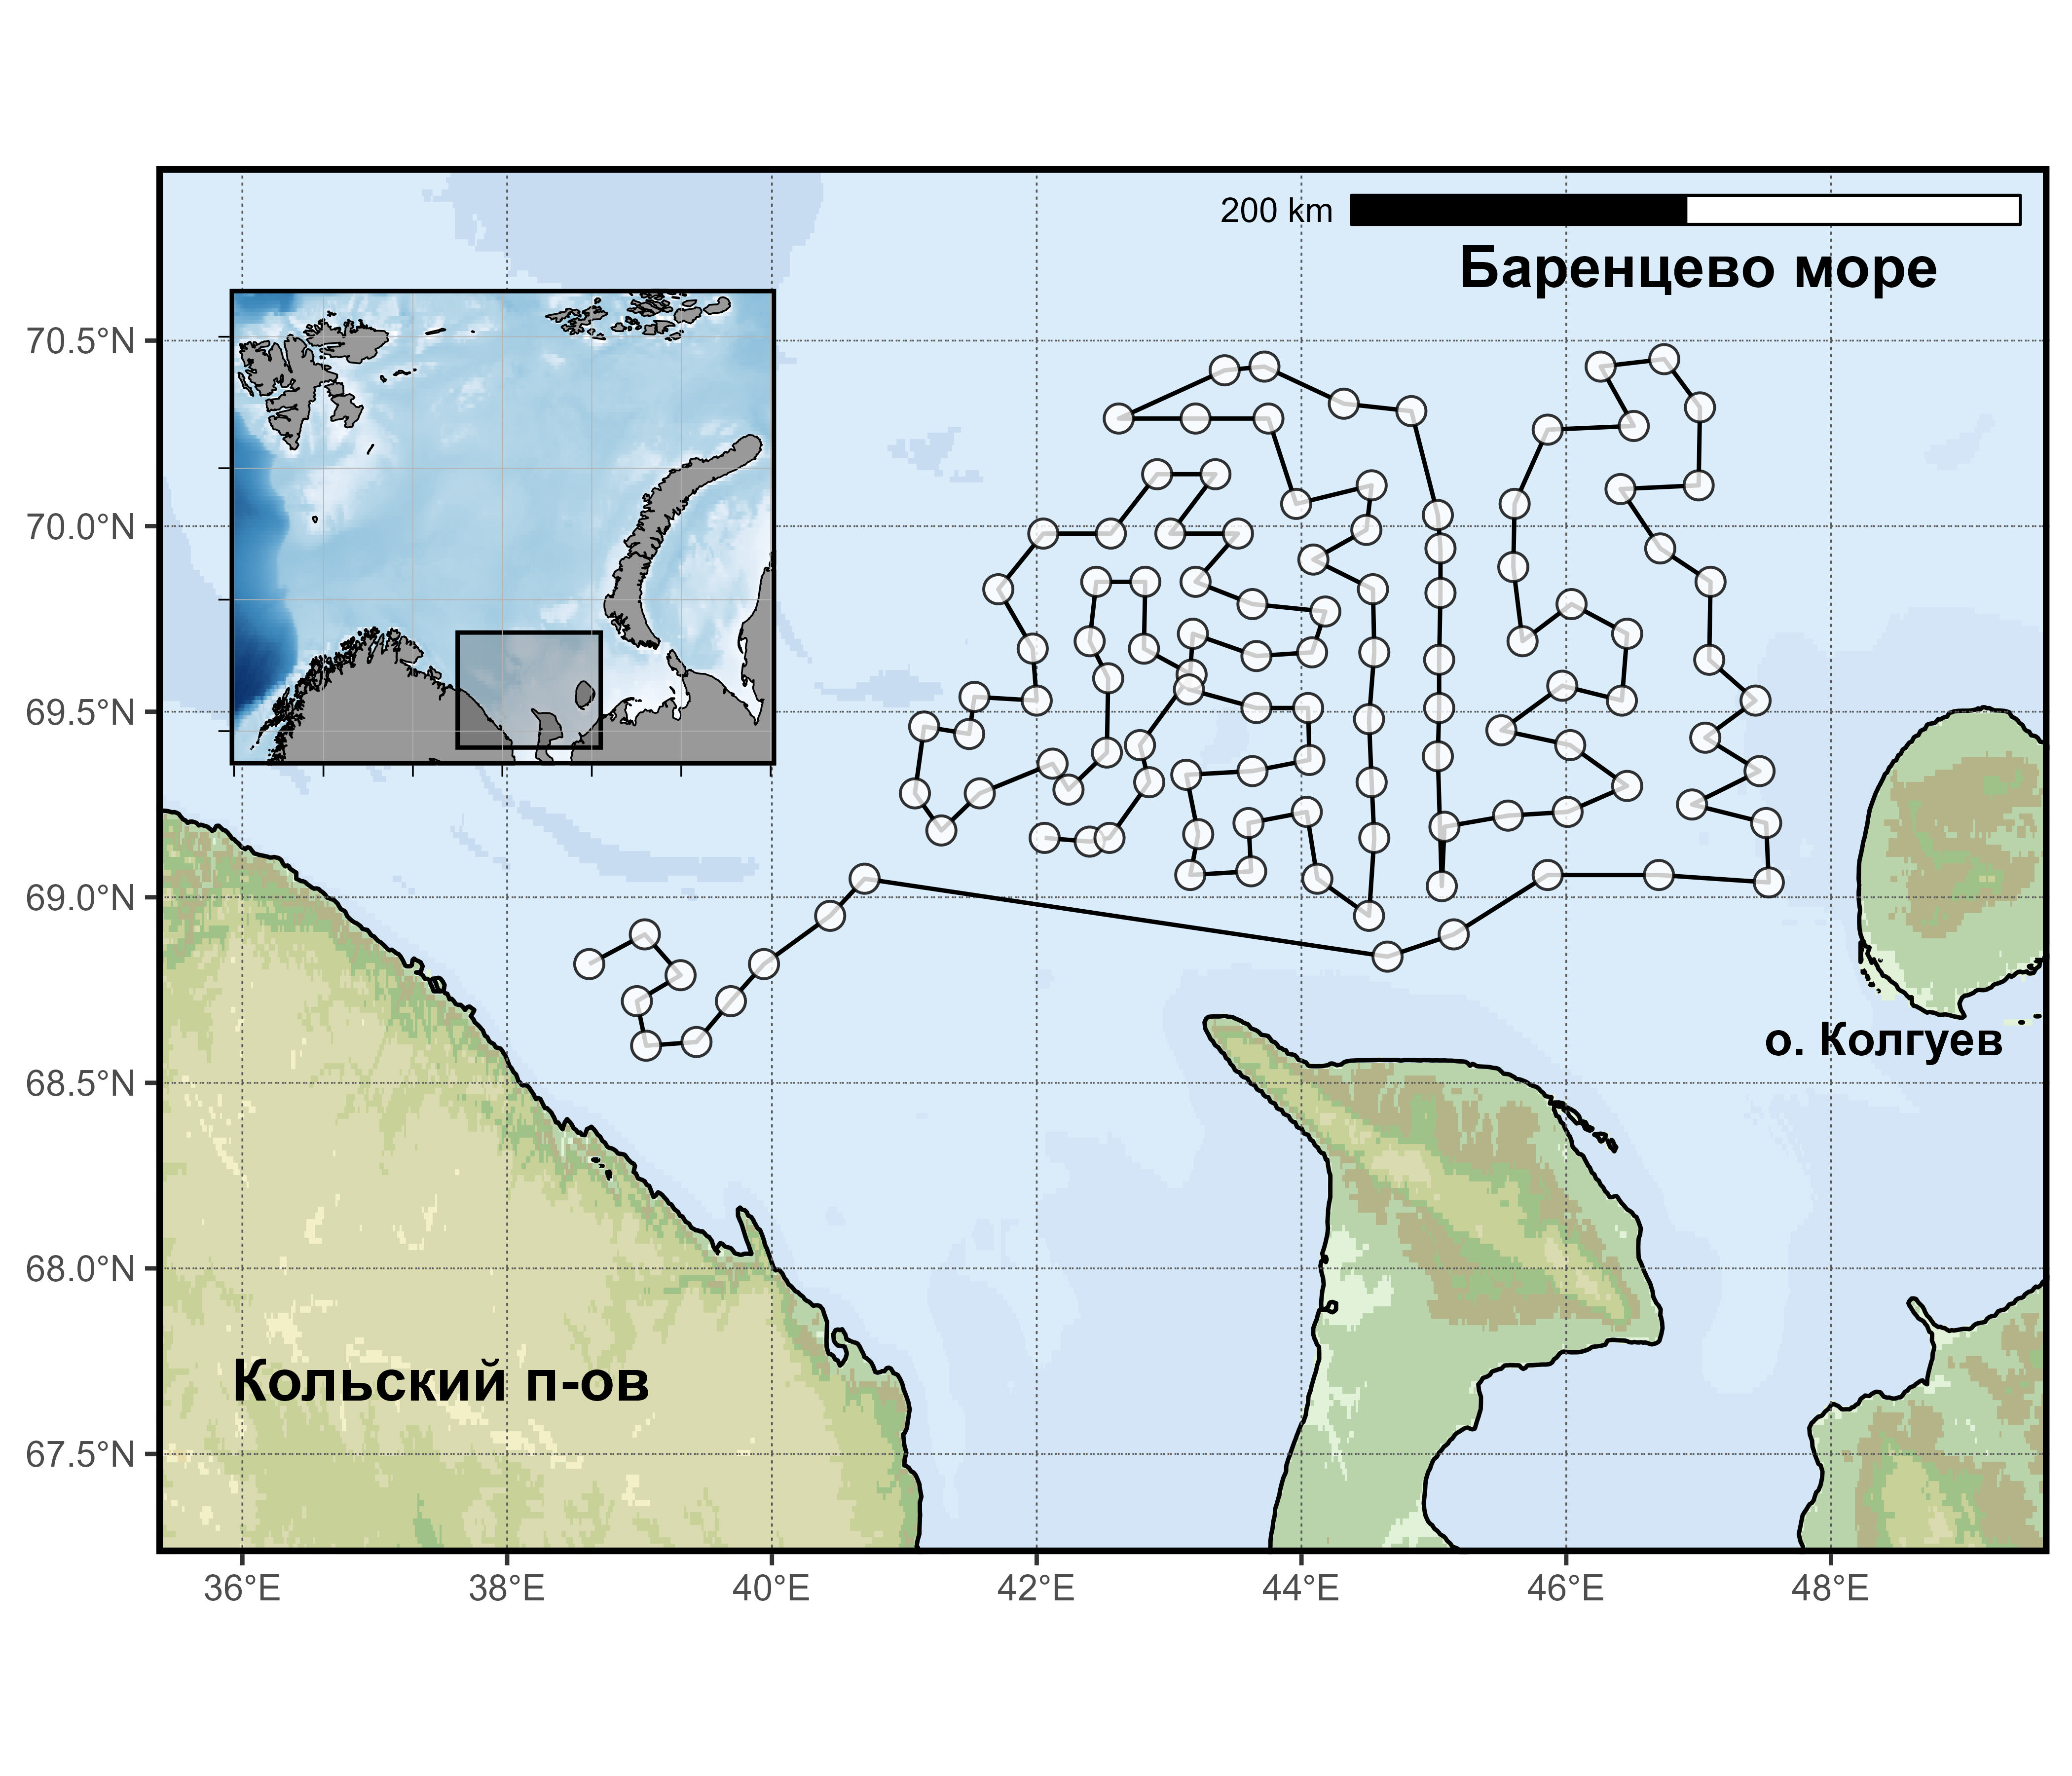
\includegraphics[width=0.8\linewidth,height=\textheight,keepaspectratio]{images/KARTOGRAPH14.PNG}

}

\caption{Рис. 14.: Карты с картой-врезкой и маршрутом}

\end{figure}%

\begin{Shaded}
\begin{Highlighting}[]
\CommentTok{\# Очистка окружения и установка рабочей директории}
\FunctionTok{rm}\NormalTok{(}\AttributeTok{list =} \FunctionTok{ls}\NormalTok{()) }\CommentTok{\# Удаление всех объектов из глобального окружения}
\FunctionTok{setwd}\NormalTok{(}\StringTok{"C:/COURSES/KARTOGRAPH/"}\NormalTok{) }\CommentTok{\# Установка рабочей директории}

\CommentTok{\# {-}{-}{-}{-}{-}{-}{-}{-}{-}{-}{-}{-}{-}{-}{-}{-}{-}}
\CommentTok{\# ЗАГРУЗКА ПАКЕТОВ}
\CommentTok{\# {-}{-}{-}{-}{-}{-}{-}{-}{-}{-}{-}{-}{-}{-}{-}{-}{-}}
\FunctionTok{library}\NormalTok{(sf)          }\CommentTok{\# Пространственные операции с векторными данными}
\FunctionTok{library}\NormalTok{(marmap)      }\CommentTok{\# Работа с батиметрическими данными (карты глубин)}
\FunctionTok{library}\NormalTok{(tidyverse)   }\CommentTok{\# Коллекция пакетов для обработки данных}
\FunctionTok{library}\NormalTok{(rnaturalearth) }\CommentTok{\# Векторные картографические данные}
\FunctionTok{library}\NormalTok{(ggspatial)   }\CommentTok{\# Инструменты для пространственной визуализации}
\FunctionTok{library}\NormalTok{(readxl)      }\CommentTok{\# Импорт данных из Excel}
\FunctionTok{library}\NormalTok{(ggOceanMaps) }\CommentTok{\# Специализированные карты океанов}
\FunctionTok{library}\NormalTok{(cowplot)     }\CommentTok{\# Компоновка графиков и добавление элементов}

\CommentTok{\# {-}{-}{-}{-}{-}{-}{-}{-}{-}{-}{-}{-}{-}{-}{-}{-}{-}}
\CommentTok{\# ЗАГРУЗКА ДАННЫХ}
\CommentTok{\# {-}{-}{-}{-}{-}{-}{-}{-}{-}{-}{-}{-}{-}{-}{-}{-}{-}}
\CommentTok{\# Чтение данных из Excel}
\NormalTok{DATA }\OtherTok{\textless{}{-}}\NormalTok{ readxl}\SpecialCharTok{::}\FunctionTok{read\_excel}\NormalTok{(}\StringTok{"KARTOGRAPHIC.xlsx"}\NormalTok{, }\AttributeTok{sheet =} \StringTok{"SURVEY"}\NormalTok{)}

\CommentTok{\# Фильтрация данных (крабовые исследования 2022)}
\NormalTok{DATA }\OtherTok{\textless{}{-}}\NormalTok{ DATA[DATA}\SpecialCharTok{$}\NormalTok{SURV }\SpecialCharTok{==} \StringTok{"CRAB"} \SpecialCharTok{\&}\NormalTok{ DATA}\SpecialCharTok{$}\NormalTok{YEAR }\SpecialCharTok{==} \DecValTok{2022}\NormalTok{, ]}

\CommentTok{\# Загрузка векторных границ России}
\NormalTok{russia\_map }\OtherTok{\textless{}{-}} \FunctionTok{ne\_states}\NormalTok{(}\AttributeTok{country =} \StringTok{"russia"}\NormalTok{, }\AttributeTok{returnclass =} \StringTok{"sf"}\NormalTok{)}

\CommentTok{\# Установка границ региона интереса}
\NormalTok{xmin }\OtherTok{\textless{}{-}} \DecValTok{35}\NormalTok{; xmax }\OtherTok{\textless{}{-}} \DecValTok{50}
\NormalTok{ymin }\OtherTok{\textless{}{-}} \FloatTok{67.2}\NormalTok{; ymax }\OtherTok{\textless{}{-}} \DecValTok{71}

\CommentTok{\# {-}{-}{-}{-}{-}{-}{-}{-}{-}{-}{-}{-}{-}{-}{-}{-}{-}}
\CommentTok{\# БАТИМЕТРИЧЕСКИЕ ДАННЫЕ}
\CommentTok{\# {-}{-}{-}{-}{-}{-}{-}{-}{-}{-}{-}{-}{-}{-}{-}{-}{-}}
\CommentTok{\# Загрузка данных о глубинах}
\NormalTok{bat }\OtherTok{\textless{}{-}} \FunctionTok{getNOAA.bathy}\NormalTok{(xmin, xmax, ymin, ymax, }\AttributeTok{resolution =} \DecValTok{1}\NormalTok{, }\AttributeTok{keep =} \ConstantTok{TRUE}\NormalTok{)}
\NormalTok{bat\_xyz }\OtherTok{\textless{}{-}} \FunctionTok{as.xyz}\NormalTok{(bat)}

\CommentTok{\# Определение цветовых уровней для глубин}
\NormalTok{breaks }\OtherTok{\textless{}{-}} \FunctionTok{c}\NormalTok{(}\SpecialCharTok{{-}}\DecValTok{10000}\NormalTok{, }\SpecialCharTok{{-}}\DecValTok{7000}\NormalTok{, }\SpecialCharTok{{-}}\DecValTok{6000}\NormalTok{, }\SpecialCharTok{{-}}\DecValTok{5000}\NormalTok{, }\SpecialCharTok{{-}}\DecValTok{4000}\NormalTok{, }\SpecialCharTok{{-}}\DecValTok{3000}\NormalTok{, }\SpecialCharTok{{-}}\DecValTok{2000}\NormalTok{, }\SpecialCharTok{{-}}\DecValTok{1000}\NormalTok{, }
            \SpecialCharTok{{-}}\DecValTok{500}\NormalTok{, }\SpecialCharTok{{-}}\DecValTok{200}\NormalTok{, }\SpecialCharTok{{-}}\DecValTok{50}\NormalTok{, }\SpecialCharTok{{-}}\DecValTok{1}\NormalTok{, }\DecValTok{5}\NormalTok{, }\DecValTok{50}\NormalTok{, }\DecValTok{100}\NormalTok{, }\DecValTok{150}\NormalTok{, }\DecValTok{200}\NormalTok{, }\DecValTok{300}\NormalTok{, }\DecValTok{400}\NormalTok{, }\DecValTok{500}\NormalTok{, }\DecValTok{1000}\NormalTok{, }\DecValTok{3000}\NormalTok{)}
\NormalTok{cols }\OtherTok{\textless{}{-}} \FunctionTok{c}\NormalTok{(}
  \StringTok{"\#5e99d6"}\NormalTok{, }\StringTok{"\#669cd4"}\NormalTok{, }\StringTok{"\#6c9fd4"}\NormalTok{, }\StringTok{"\#96bce3"}\NormalTok{, }\StringTok{"\#AEC8E3"}\NormalTok{, }\StringTok{"\#a6c4e3"}\NormalTok{,}
  \StringTok{"\#AEC8E3"}\NormalTok{, }\StringTok{"\#BBD0EB"}\NormalTok{, }\StringTok{"\#C7DCF1"}\NormalTok{, }\StringTok{"\#DAECFA"}\NormalTok{, }\StringTok{"\#D2E5F6"}\NormalTok{, }\StringTok{"\#e1f2d8"}\NormalTok{,}
  \StringTok{"\#B8D3AA"}\NormalTok{, }\StringTok{"\#b3b387"}\NormalTok{, }\StringTok{"\#9EC187"}\NormalTok{, }\StringTok{"\#C7D097"}\NormalTok{, }\StringTok{"\#DADBAF"}\NormalTok{, }\StringTok{"\#F3F0C7"}\NormalTok{,}
  \StringTok{"\#E6DBA8"}\NormalTok{, }\StringTok{"\#DACFA1"}\NormalTok{, }\StringTok{"\#D1BF81"}\NormalTok{, }\StringTok{"\#C69D45"}
\NormalTok{)}

\CommentTok{\# Категоризация глубин}
\NormalTok{bat\_xyz}\SpecialCharTok{$}\NormalTok{V4 }\OtherTok{\textless{}{-}} \FunctionTok{cut}\NormalTok{(bat\_xyz}\SpecialCharTok{$}\NormalTok{V3, }\AttributeTok{breaks =}\NormalTok{ breaks)}
\NormalTok{niveles }\OtherTok{\textless{}{-}} \FunctionTok{levels}\NormalTok{(bat\_xyz}\SpecialCharTok{$}\NormalTok{V4)}

\CommentTok{\# Создание координатной сетки}
\NormalTok{ga\_grid }\OtherTok{\textless{}{-}}\NormalTok{ russia\_map }\SpecialCharTok{\%\textgreater{}\%} 
  \FunctionTok{st\_make\_grid}\NormalTok{(}\AttributeTok{cellsize =} \FunctionTok{c}\NormalTok{(}\DecValTok{2}\NormalTok{, }\FloatTok{0.5}\NormalTok{), }\AttributeTok{offset =} \FunctionTok{c}\NormalTok{(}\DecValTok{34}\NormalTok{, }\DecValTok{67}\NormalTok{))}

\CommentTok{\# {-}{-}{-}{-}{-}{-}{-}{-}{-}{-}{-}{-}{-}{-}{-}{-}{-}}
\CommentTok{\# ПОСТРОЕНИЕ ОСНОВНОЙ КАРТЫ}
\CommentTok{\# {-}{-}{-}{-}{-}{-}{-}{-}{-}{-}{-}{-}{-}{-}{-}{-}{-}}
\NormalTok{map }\OtherTok{\textless{}{-}} \FunctionTok{ggplot}\NormalTok{() }\SpecialCharTok{+}
  \CommentTok{\# Векторные границы России}
  \FunctionTok{geom\_sf}\NormalTok{(}\AttributeTok{data =}\NormalTok{ russia\_map) }\SpecialCharTok{+}
  \CommentTok{\# Батиметрическая подложка}
  \FunctionTok{geom\_tile}\NormalTok{(}\AttributeTok{data =}\NormalTok{ bat\_xyz, }\FunctionTok{aes}\NormalTok{(}\AttributeTok{x =}\NormalTok{ V1, }\AttributeTok{y =}\NormalTok{ V2, }\AttributeTok{fill =}\NormalTok{ V4), }\AttributeTok{show.legend =} \ConstantTok{FALSE}\NormalTok{) }\SpecialCharTok{+}
  \FunctionTok{scale\_fill\_manual}\NormalTok{(}\AttributeTok{values =}\NormalTok{ cols, }\AttributeTok{breaks =}\NormalTok{ niveles) }\SpecialCharTok{+}
  \CommentTok{\# Контур нулевой глубины (береговая линия)}
  \FunctionTok{geom\_contour}\NormalTok{(}\AttributeTok{data =}\NormalTok{ bat\_xyz, }\FunctionTok{aes}\NormalTok{(}\AttributeTok{x =}\NormalTok{ V1, }\AttributeTok{y =}\NormalTok{ V2, }\AttributeTok{z =}\NormalTok{ V3), }
               \AttributeTok{breaks =} \DecValTok{0}\NormalTok{, }\AttributeTok{color =} \StringTok{"black"}\NormalTok{, }\AttributeTok{linewidth =} \FloatTok{0.5}\NormalTok{) }\SpecialCharTok{+} 
  \CommentTok{\# Координатная сетка}
  \FunctionTok{geom\_sf}\NormalTok{(}\AttributeTok{data =}\NormalTok{ ga\_grid, }\AttributeTok{alpha =} \FloatTok{0.01}\NormalTok{, }\AttributeTok{linetype =} \DecValTok{3}\NormalTok{) }\SpecialCharTok{+}
  \CommentTok{\# Ограничение области карты}
  \FunctionTok{coord\_sf}\NormalTok{(}\AttributeTok{xlim =} \FunctionTok{c}\NormalTok{(}\DecValTok{36}\NormalTok{, }\DecValTok{49}\NormalTok{), }\AttributeTok{ylim =} \FunctionTok{c}\NormalTok{(}\FloatTok{67.4}\NormalTok{, }\FloatTok{70.8}\NormalTok{)) }\SpecialCharTok{+} 
  \CommentTok{\# Масштабная линейка}
  \FunctionTok{annotation\_scale}\NormalTok{(}\AttributeTok{location =} \StringTok{"tr"}\NormalTok{, }\AttributeTok{width\_hint =} \FloatTok{0.5}\NormalTok{) }\SpecialCharTok{+}
  \FunctionTok{labs}\NormalTok{(}\AttributeTok{x =} \ConstantTok{NULL}\NormalTok{, }\AttributeTok{y =} \ConstantTok{NULL}\NormalTok{) }\SpecialCharTok{+}
  \CommentTok{\# Географические подписи}
  \FunctionTok{annotate}\NormalTok{(}\StringTok{"text"}\NormalTok{, }\AttributeTok{x =} \DecValTok{47}\NormalTok{, }\AttributeTok{y =} \FloatTok{70.7}\NormalTok{, }\AttributeTok{size =} \DecValTok{5}\NormalTok{, }
           \AttributeTok{label =} \StringTok{"Баренцево море"}\NormalTok{, }\AttributeTok{fontface =} \StringTok{"bold"}\NormalTok{) }\SpecialCharTok{+}
  \FunctionTok{annotate}\NormalTok{(}\StringTok{"text"}\NormalTok{, }\AttributeTok{x =} \FloatTok{48.4}\NormalTok{, }\AttributeTok{y =} \FloatTok{68.62}\NormalTok{, }\AttributeTok{size =} \DecValTok{4}\NormalTok{,}
           \AttributeTok{label =} \StringTok{"о. Колгуев"}\NormalTok{, }\AttributeTok{fontface =} \StringTok{"bold"}\NormalTok{) }\SpecialCharTok{+}
  \FunctionTok{annotate}\NormalTok{(}\StringTok{"text"}\NormalTok{, }\AttributeTok{x =} \FloatTok{37.5}\NormalTok{, }\AttributeTok{y =} \FloatTok{67.7}\NormalTok{, }\AttributeTok{size =} \DecValTok{5}\NormalTok{,}
           \AttributeTok{label =} \StringTok{"Кольский п{-}ов"}\NormalTok{, }\AttributeTok{fontface =} \StringTok{"bold"}\NormalTok{) }\SpecialCharTok{+}
  \CommentTok{\# Маршрут и точки исследований}
  \FunctionTok{geom\_path}\NormalTok{(}\AttributeTok{data =}\NormalTok{ DATA, }\FunctionTok{aes}\NormalTok{(}\AttributeTok{x =}\NormalTok{ X, }\AttributeTok{y =}\NormalTok{ Y), }\AttributeTok{color =} \StringTok{"black"}\NormalTok{) }\SpecialCharTok{+}
  \FunctionTok{geom\_point}\NormalTok{(}\AttributeTok{data =}\NormalTok{ DATA, }\FunctionTok{aes}\NormalTok{(}\AttributeTok{x =}\NormalTok{ X, }\AttributeTok{y =}\NormalTok{ Y), }
             \AttributeTok{size =} \DecValTok{3}\NormalTok{, }\AttributeTok{color =} \StringTok{"black"}\NormalTok{, }\AttributeTok{fill =} \StringTok{"white"}\NormalTok{, }
             \AttributeTok{shape =} \DecValTok{21}\NormalTok{, }\AttributeTok{alpha =} \FloatTok{0.8}\NormalTok{) }\SpecialCharTok{+}
  \CommentTok{\# ДОБАВЛЕНИЕ РАМКИ {-} ключевое изменение}
  \FunctionTok{theme}\NormalTok{(}\AttributeTok{panel.border =} \FunctionTok{element\_rect}\NormalTok{(}\AttributeTok{colour =} \StringTok{"black"}\NormalTok{, }\AttributeTok{fill =} \ConstantTok{NA}\NormalTok{, }\AttributeTok{linewidth =} \FloatTok{1.5}\NormalTok{))}

\CommentTok{\# {-}{-}{-}{-}{-}{-}{-}{-}{-}{-}{-}{-}{-}{-}{-}{-}{-}}
\CommentTok{\# СОЗДАНИЕ ВСТАВКИ{-}ЛОКАЦИИ}
\CommentTok{\# {-}{-}{-}{-}{-}{-}{-}{-}{-}{-}{-}{-}{-}{-}{-}{-}{-}}
\CommentTok{\# Область для вставки}
\NormalTok{ins }\OtherTok{\textless{}{-}} \FunctionTok{data.frame}\NormalTok{(}\AttributeTok{lon =} \FunctionTok{c}\NormalTok{(}\DecValTok{10}\NormalTok{, }\DecValTok{10}\NormalTok{, }\DecValTok{70}\NormalTok{, }\DecValTok{70}\NormalTok{), }\AttributeTok{lat =} \FunctionTok{c}\NormalTok{(}\DecValTok{67}\NormalTok{, }\DecValTok{80}\NormalTok{, }\DecValTok{80}\NormalTok{, }\DecValTok{67}\NormalTok{))}

\CommentTok{\# Получение данных для вставки}
\NormalTok{mar\_bathy }\OtherTok{\textless{}{-}} \FunctionTok{getNOAA.bathy}\NormalTok{(}\DecValTok{9}\NormalTok{, }\DecValTok{71}\NormalTok{, }\FloatTok{66.5}\NormalTok{, }\DecValTok{83}\NormalTok{, }\AttributeTok{res =} \DecValTok{4}\NormalTok{, }\AttributeTok{keep =} \ConstantTok{TRUE}\NormalTok{)}
\NormalTok{bathy }\OtherTok{\textless{}{-}} \FunctionTok{raster\_bathymetry}\NormalTok{(stars}\SpecialCharTok{::}\FunctionTok{st\_as\_stars}\NormalTok{(marmap}\SpecialCharTok{::}\FunctionTok{as.raster}\NormalTok{(mar\_bathy)), }
                           \AttributeTok{depths =} \ConstantTok{NULL}\NormalTok{, }\AttributeTok{verbose =} \ConstantTok{FALSE}\NormalTok{)}

\CommentTok{\# Построение вставки}
\NormalTok{insetmap }\OtherTok{\textless{}{-}} \FunctionTok{basemap}\NormalTok{(ins, }\AttributeTok{shapefiles =} \FunctionTok{list}\NormalTok{(}\AttributeTok{land =}\NormalTok{ dd\_land, }\AttributeTok{bathy =}\NormalTok{ bathy), }
                   \AttributeTok{bathy.style =} \StringTok{"rub"}\NormalTok{, }\AttributeTok{legends =} \ConstantTok{FALSE}\NormalTok{) }\SpecialCharTok{+}
  \CommentTok{\# Прямоугольник, обозначающий область основной карты}
  \FunctionTok{geom\_rect}\NormalTok{(}\FunctionTok{aes}\NormalTok{(}\AttributeTok{xmin =} \DecValTok{35}\NormalTok{, }\AttributeTok{xmax =} \DecValTok{51}\NormalTok{, }\AttributeTok{ymin =} \FloatTok{67.5}\NormalTok{, }\AttributeTok{ymax =} \DecValTok{71}\NormalTok{), }
            \AttributeTok{fill =} \StringTok{"black"}\NormalTok{, }\AttributeTok{color =} \StringTok{"black"}\NormalTok{, }\AttributeTok{alpha =} \FloatTok{0.2}\NormalTok{) }\SpecialCharTok{+}
  \FunctionTok{labs}\NormalTok{(}\AttributeTok{y =} \ConstantTok{NULL}\NormalTok{, }\AttributeTok{x =} \ConstantTok{NULL}\NormalTok{) }\SpecialCharTok{+}
  \CommentTok{\# Упрощение оформления}
  \FunctionTok{theme}\NormalTok{(}\AttributeTok{axis.text.x =} \FunctionTok{element\_blank}\NormalTok{(), }
        \AttributeTok{axis.text.y =} \FunctionTok{element\_blank}\NormalTok{(),}
        \CommentTok{\# Рамка для вставки}
        \AttributeTok{panel.border =} \FunctionTok{element\_rect}\NormalTok{(}\AttributeTok{colour =} \StringTok{"black"}\NormalTok{, }\AttributeTok{fill =} \ConstantTok{NA}\NormalTok{, }\AttributeTok{linewidth =} \DecValTok{1}\NormalTok{))}

\CommentTok{\# {-}{-}{-}{-}{-}{-}{-}{-}{-}{-}{-}{-}{-}{-}{-}{-}{-}}
\CommentTok{\# ФИНАЛЬНАЯ КОМПОНОВКА С РАМКОЙ}
\CommentTok{\# {-}{-}{-}{-}{-}{-}{-}{-}{-}{-}{-}{-}{-}{-}{-}{-}{-}}
\NormalTok{MAP }\OtherTok{\textless{}{-}} \FunctionTok{ggdraw}\NormalTok{() }\SpecialCharTok{+}
  \CommentTok{\# Основная карта}
  \FunctionTok{draw\_plot}\NormalTok{(map) }\SpecialCharTok{+}
  \CommentTok{\# Вставка с позиционированием}
  \FunctionTok{draw\_plot}\NormalTok{(insetmap,}
            \AttributeTok{height =} \FloatTok{0.3}\NormalTok{,}
            \AttributeTok{x =} \SpecialCharTok{{-}}\FloatTok{0.26}\NormalTok{,}
            \AttributeTok{y =} \FloatTok{0.55}\NormalTok{) }\SpecialCharTok{+}
  \CommentTok{\# ДОБАВЛЕНИЕ РАМКИ ВОКРУГ ВСЕЙ КОМПОЗИЦИИ}
  \FunctionTok{theme}\NormalTok{(}\AttributeTok{plot.background =} \FunctionTok{element\_rect}\NormalTok{(}\AttributeTok{colour =} \StringTok{"black"}\NormalTok{, }\AttributeTok{fill =} \ConstantTok{NA}\NormalTok{, }\AttributeTok{linewidth =} \DecValTok{2}\NormalTok{))}

\CommentTok{\# Вывод финальной карты}
\FunctionTok{print}\NormalTok{(MAP)}

\CommentTok{\# {-}{-}{-}{-}{-}{-}{-}{-}{-}{-}{-}{-}{-}{-}{-}{-}{-}}
\CommentTok{\# СОХРАНЕНИЕ РЕЗУЛЬТАТА}
\CommentTok{\# {-}{-}{-}{-}{-}{-}{-}{-}{-}{-}{-}{-}{-}{-}{-}{-}{-}}
\FunctionTok{ggsave}\NormalTok{(}\StringTok{"DATA\_MAP\_FRAMED.jpg"}\NormalTok{, }
       \AttributeTok{plot =}\NormalTok{ MAP,}
       \AttributeTok{device =} \StringTok{"jpeg"}\NormalTok{, }
       \AttributeTok{dpi =} \DecValTok{600}\NormalTok{,}
       \AttributeTok{width =} \DecValTok{9}\NormalTok{,}
       \AttributeTok{height =} \DecValTok{7}\NormalTok{,}
       \AttributeTok{units =} \StringTok{"in"}\NormalTok{)}
\end{Highlighting}
\end{Shaded}

\bookmarksetup{startatroot}

\chapter{SDM - Модели пространственного распределения
видов}\label{sdm---ux43cux43eux434ux435ux43bux438-ux43fux440ux43eux441ux442ux440ux430ux43dux441ux442ux432ux435ux43dux43dux43eux433ux43e-ux440ux430ux441ux43fux440ux435ux434ux435ux43bux435ux43dux438ux44f-ux432ux438ux434ux43eux432}

\section{Введение}\label{ux432ux432ux435ux434ux435ux43dux438ux435-3}

\section{Загрузка данных и первичный
осмотр}\label{ux437ux430ux433ux440ux443ux437ux43aux430-ux434ux430ux43dux43dux44bux445-ux438-ux43fux435ux440ux432ux438ux447ux43dux44bux439-ux43eux441ux43cux43eux442ux440-1}

Текст. Текст. Текст.

\section{Описательная статистика и
визуализация}\label{ux43eux43fux438ux441ux430ux442ux435ux43bux44cux43dux430ux44f-ux441ux442ux430ux442ux438ux441ux442ux438ux43aux430-ux438-ux432ux438ux437ux443ux430ux43bux438ux437ux430ux446ux438ux44f-1}

Текст. Текст. Текст.

\bookmarksetup{startatroot}

\chapter{Основы
геостатистики}\label{ux43eux441ux43dux43eux432ux44b-ux433ux435ux43eux441ux442ux430ux442ux438ux441ux442ux438ux43aux438}

\section{Введение}\label{ux432ux432ux435ux434ux435ux43dux438ux435-4}

\section{Загрузка данных и первичный
осмотр}\label{ux437ux430ux433ux440ux443ux437ux43aux430-ux434ux430ux43dux43dux44bux445-ux438-ux43fux435ux440ux432ux438ux447ux43dux44bux439-ux43eux441ux43cux43eux442ux440-2}

Текст. Текст. Текст.

\section{Описательная статистика и
визуализация}\label{ux43eux43fux438ux441ux430ux442ux435ux43bux44cux43dux430ux44f-ux441ux442ux430ux442ux438ux441ux442ux438ux43aux430-ux438-ux432ux438ux437ux443ux430ux43bux438ux437ux430ux446ux438ux44f-2}

Текст. Текст. Текст.

\bookmarksetup{startatroot}

\chapter{Байесовский
подход}\label{ux431ux430ux439ux435ux441ux43eux432ux441ux43aux438ux439-ux43fux43eux434ux445ux43eux434}

\section{Лекция-Введение}\label{ux43bux435ux43aux446ux438ux44f-ux432ux432ux435ux434ux435ux43dux438ux435}

\[  
P(\theta|x)=\frac{L(x|\theta)P(\theta)}{\sum\limits_{i=1}^{n}{\left[ L(x_i|\theta)P(\theta)\right]}}  
\]

\section{Описательная статистика и
визуализация}\label{ux43eux43fux438ux441ux430ux442ux435ux43bux44cux43dux430ux44f-ux441ux442ux430ux442ux438ux441ux442ux438ux43aux430-ux438-ux432ux438ux437ux443ux430ux43bux438ux437ux430ux446ux438ux44f-3}

Текст. Текст. Текст.

\bookmarksetup{startatroot}

\chapter{Продукционные
модели}\label{ux43fux440ux43eux434ux443ux43aux446ux438ux43eux43dux43dux44bux435-ux43cux43eux434ux435ux43bux438}

\section{Введение}\label{ux432ux432ux435ux434ux435ux43dux438ux435-5}

\section{Загрузка данных и первичный
осмотр}\label{ux437ux430ux433ux440ux443ux437ux43aux430-ux434ux430ux43dux43dux44bux445-ux438-ux43fux435ux440ux432ux438ux447ux43dux44bux439-ux43eux441ux43cux43eux442ux440-3}

Текст. Текст. Текст.

\section{Описательная статистика и
визуализация}\label{ux43eux43fux438ux441ux430ux442ux435ux43bux44cux43dux430ux44f-ux441ux442ux430ux442ux438ux441ux442ux438ux43aux430-ux438-ux432ux438ux437ux443ux430ux43bux438ux437ux430ux446ux438ux44f-4}

Текст. Текст. Текст.

\bookmarksetup{startatroot}

\chapter{Введение в
прогнозирование}\label{ux432ux432ux435ux434ux435ux43dux438ux435-ux432-ux43fux440ux43eux433ux43dux43eux437ux438ux440ux43eux432ux430ux43dux438ux435}

\section{Введение}\label{ux432ux432ux435ux434ux435ux43dux438ux435-6}

\section{Загрузка данных и первичный
осмотр}\label{ux437ux430ux433ux440ux443ux437ux43aux430-ux434ux430ux43dux43dux44bux445-ux438-ux43fux435ux440ux432ux438ux447ux43dux44bux439-ux43eux441ux43cux43eux442ux440-4}

Текст. Текст. Текст.

\section{Описательная статистика и
визуализация}\label{ux43eux43fux438ux441ux430ux442ux435ux43bux44cux43dux430ux44f-ux441ux442ux430ux442ux438ux441ux442ux438ux43aux430-ux438-ux432ux438ux437ux443ux430ux43bux438ux437ux430ux446ux438ux44f-5}

Текст. Текст. Текст.

\bookmarksetup{startatroot}

\chapter{ПРП и стратегии
управления}\label{ux43fux440ux43f-ux438-ux441ux442ux440ux430ux442ux435ux433ux438ux438-ux443ux43fux440ux430ux432ux43bux435ux43dux438ux44f}

\section{Введение}\label{ux432ux432ux435ux434ux435ux43dux438ux435-7}

\section{Загрузка данных и первичный
осмотр}\label{ux437ux430ux433ux440ux443ux437ux43aux430-ux434ux430ux43dux43dux44bux445-ux438-ux43fux435ux440ux432ux438ux447ux43dux44bux439-ux43eux441ux43cux43eux442ux440-5}

Текст. Текст. Текст.

\section{Описательная статистика и
визуализация}\label{ux43eux43fux438ux441ux430ux442ux435ux43bux44cux43dux430ux44f-ux441ux442ux430ux442ux438ux441ux442ux438ux43aux430-ux438-ux432ux438ux437ux443ux430ux43bux438ux437ux430ux446ux438ux44f-6}

Текст. Текст. Текст.

\bookmarksetup{startatroot}

\chapter*{References}\label{references}
\addcontentsline{toc}{chapter}{References}

\markboth{References}{References}

\phantomsection\label{refs}




\end{document}
